\documentclass[showtrims,		% Mostra as marcas de corte em cruz
			   trimframe,		% Mostra as marcas de corte em linha, para conferência
			   12pt				% 8pt, 9pt, 10pt, 11pt, 12pt, 14pt, 17pt, 20pt 
			   ]{memoir}
\usepackage[brazilian,
			% english,
			% italian,
			% ngerman,
			% french,
			% russian,
			% polutonikogreek
			]{babel}
\usepackage{anyfontsize}			    % para tamanhos de fontes maiores que \Huge 
\usepackage{relsize}					% para aumentar ou diminuir fonte por pontos. Ex. \smaller[1]
\usepackage{fontspec}					% para rodar fontes do sistema
\usepackage[switch]{lineno} 			% para numerar linhas
\usepackage{lipsum}						% para colocar textos lipsum
\usepackage{alltt}						% para colocar espaços duplos. Ex: verso livre
\usepackage{graphicx}					% para colocar imagens
\usepackage{float}						% para flutuar imagens e tabelas 		
\usepackage{lettrine}					% para capsulares
\usepackage{comment}					% para comentar o código em bloco \begin{comment}...
\usepackage{adforn}						% para adornos & glyphs
\usepackage{xcolor}					 	% para texto colorido
\usepackage[babel]{microtype}			% para ajustes finos na mancha
\usepackage{enumerate,enumitem}			% para tipos diferentes de enumeração/formatação ver `edlab-extra.sty`
\usepackage{marginnote}					% para notas laterais
\usepackage{titlesec}					% para produzir os distanciamentos entre pontos no \dotfill

%\usepackage{makeidx} 					% para índice remissivo

\usepackage{edlab-penalties}
\usepackage{edlab-git}
\usepackage{edlab-toc}					% define sumário
\usepackage{edlab-extra}				% define epígrafe, quote
\usepackage[14x21]{edlab-margins}
\usepackage[%semcabeco, 				% para remover cabeço, sobe mancha e mantem estilos
			]{edlab-sections}			% define pagestyle (cabeço, rodapé e seções)
\usepackage[%
			% notasemlinha 			
			% notalinhalonga
			chicagofootnotes			% para notas com número e ponto cf. man. de Chicago
			]{edlab-footnotes}


% Medidas (ver: memoir p.11 fig.2.3)
\parindent=3ex			% Tamanho da indentação
\parskip=0pt			% Entre parágrafos
\marginparsep=1em		% Entre mancha e nota lateral 
\marginparwidth=4em		% Tamanho da caixa de texto da nota laterial

% Fontes
\newfontfamily\formular{Formular}
\newfontfamily\formularlight{Formular Light}
\setmainfont[Ligatures=TeX,Numbers=OldStyle]{Linux Libertine O}


% Estilos
\makeoddhead{baruch}{}{\scshape\MakeLowercase{\scshape\MakeTextLowercase{\leftmark}}}{}
\makeevenhead{baruch}{}{\scshape\MakeLowercase{\parttitle}}{}
\makeevenfoot{baruch}{}{\footnotesize\thepage}{}
\makeoddfoot{baruch}{}{\footnotesize\thepage}{}
\pagestyle{baruch}		
\headstyles{baruch}

% Testes


\begin{document}


%\book{\textsc{Testis nossis},  Mussum Ipsum}

\part{Amor é fogo que arde sem se ver}

\chapter{É um não querer mais que bem\footnote{Cacilds vidis litro abertis.} querer}

\newcommand{\pacote}[1]{\marginnote{\tiny\alltt{#1}}}


\pacote{edlab-extra}
\begin{epigraphs} 
\qitem{Cogitatio in vero exquirendo maxime versatur. 
		 Appetitus impellit ad agendum.}{\textsc{Marcus
		  Tullius Cicero}}
\end{epigraphs}

\pacote{lettrine.sty}
\lettrine[realheight]{\textcolor{red}{M}}{ussum Ipsum}, cacilds vidis litro abertis. Suco de cevadiss, é um leite
divinis, qui tem lupuliz, a\textcolor{green}{fi}matis, aguis e fermentis. Sapien in monti palavris
qui num significa nadis i pareci latim.  Diuretics paradis num copo é motivis
de denguis. Mauris nec dolor in eros commodo tempor. Aenean aliquam molestie
leo, vitae iaculis nisl. Ligue para \textcolor{green}{9-3129-4563}.


In elementis mé pra quem é amistosis quis leo. Vehicula non. Ut sed ex eros.
Vivamus sit amet nibh non tellus tristique interdum. Copo furadis é disculpa de
bebadis, arcu quam euismod magna. Todo mundo vê os porris que eu tomo, mas
ninguém vê os tombis que eu levo!

\section{É solitário andar por entre a gente}


Pra lá , depois divoltis porris, paradis. Praesent vel viverra nisi. Mauris
aliquet nunc non turpis scelerisque, eget. Nec orci ornare consequat. Praesent
lacinia ultrices\footnote{Praesent vel viverra nisi. Mauris
aliquet nunc non turpis scelerisque, eget.} consectetur.\footnote{Sed non ipsum.} Sed non ipsum felis. Si u mundo tá muito paradis?
Toma um mé que o mundo vai girarzis!\footnote{\textsc{Mussum}, Ipsum,
\textit{Cacilds vidis litro abertis}.}




Em pé sem cair, deitado sem dormir, sentado sem cochilar e fazendo pose. Quem
num gosta di mé, boa gentis num é. Não sou faixa preta cumpadi, sou preto
inteiris, inteiris. Aenean aliquam molestie leo, vitae iaculis nisl.

\settowidth{\versewidth}{Nay, nay, I leave thee not, thou goest too}
\begin{verse}[\versewidth]
\ldots \\*
His judgement rendered, he dissolved the Thing. \\*
\flagverse{Ingeborg} And your decision? \\*
\flagverse{Fridthjof} \vinphantom{And your decision?}
Have I ought to choose? \\*
Is not mine honour bound by his decree? \\*
And that I will redeem through Angantyr \\*
His paltry gold doth hide in Nastrand’s flood. \\*
Today will I depart. \\*
\flagverse{Ingeborg} \vinphantom{Today will I depart.}
And Ingeborg leave? \\*
\flagverse{Fridthjof} Nay, nay, I leave thee not,
thou goest too. \\*
\flagverse{Ingeborg} Impossible! \\*
\flagverse{Fridthjof} \vinphantom{Impossible!}
O! hear me, ere thou answerest.
\end{verse}

Interagi no mé, cursus quis, vehicula ac nisi. Admodum accumsan disputationi eu
sit. Vide electram sadipscing et per. Detraxit consequat et quo num tendi nada.
Atirei o pau no gatis, per gatis num morreus.

Suco de cevadiss deixa as pessoas mais interessantis. Tá deprimidis, eu conheço
uma cachacis que pode alegrar sua vidis. Praesent malesuada urna nisi, quis
volutpat erat hendrerit non. Nam vulputate dapibus. Quem manda na minha terra
sou euzis!

\subsection{É nunca contentar-se de contente}

Em pé sem cair, deitado sem dormir, sentado sem cochilar e fazendo pose. Quem
num gosta di mé, boa gentis num é. Não sou faixa preta cumpadi, sou preto
inteiris, inteiris. Aenean aliquam molestie leo, vitae iaculis nisl.

Interagi no mé, cursus quis, vehicula ac nisi. Admodum accumsan disputationi eu
sit. Vide electram sadipscing et per. Detraxit consequat et quo num tendi nada.
Atirei o pau no gatis, per gatis num morreus.

\pacote{alltt}
\begin{alltt}\normalfont			%Verso branco
I used to love my garden
But now my love is dead
   For I found a 
   			      		[ bachelor’s button
   In black-eyed 
              	        [ Susan’s bed.
\end{alltt}

Suco de cevadiss deixa as pessoas mais interessantis. Tá deprimidis, eu conheço
uma cachacis que pode alegrar sua vidis. Praesent malesuada urna nisi, quis
volutpat erat hendrerit non. Nam vulputate dapibus. Quem manda na minha terra
sou euzis!

\subsubsection{Posuere libero varius}

Mussum Ipsum, cacilds vidis litro abertis. Posuere libero varius. Nullam a nisl
ut ante blandit hendrerit. Aenean sit amet nisi. Mé faiz elementum girarzis,
nisi eros vermeio. Interessantiss quisso pudia ce receita de bolis, mais bolis
eu num gostis. Diuretics paradis num copo é motivis de denguis.

Per aumento de cachacis, eu reclamis. Todo mundo vê os porris que eu tomo, mas
ninguém vê os tombis que eu levo! Admodum accumsan disputationi eu sit. Vide
electram sadipscing et per. Detraxit consequat et quo num tendi nada.

\chapter{Leite de capivaris, leite de mula manquis sem cabeça}

Leite de capivaris, leite de mula manquis sem cabeça. Suco de cevadiss deixa as
pessoas mais interessantis. Casamentiss faiz malandris se pirulitá. Em pé sem
cair, deitado sem dormir, sentado sem cochilar e fazendo pose.

Praesent vel viverra nisi. Mauris aliquet nunc non turpis scelerisque, eget.
Atirei o pau no gatis, per gatis num morreus. Quem num gosta di mé, boa gentis
num é. Paisis, filhis, espiritis santis.

\settowidth{\versewidth}{É solitário andar por entre a gente;}\label{camoes}
\begin{verse}[\versewidth]
\linenumbers

Amor é fogo que arde sem se ver;\\*
É ferida que dói e não se sente;\\*
É um contentamento descontente;\\*
É dor que desatina sem doer;\\!

É um não querer mais que bem querer;\\*
É solitário andar por entre a gente;\\*
É nunca contentar-se de contente;\\*
É cuidar que se ganha em se perder;\\!

É querer estar preso por vontade;\\*
É servir a quem vence, o vencedor;\\*
É ter com quem nos mata lealdade.\\!

Mas como causar pode seu favor\\*
Nos corações humanos amizade,\\*
Se tão contrário a si é o mesmo Amor?\\!

                 \hfill    \textsc{Luís de Camões}
\end{verse}

\marginnote{\footnotesize \textcolor{green}{Pra lá, depois divoltis porris, paradis. Praesent vel viverra nisi.}}
Delegadis gente finis, bibendum egestas augue arcu ut est. Praesent malesuada
urna nisi, quis volutpat erat hendrerit non. Nam vulputate dapibus. Nullam
volutpat risus nec leo commodo, ut interdum diam laoreet. Sed non consequat
odio. Si num tem leite então bota uma pinga aí cumpadi!

Sapien in monti palavris qui num significa nadis i pareci latim.  Quem num
gosta di mim que vai caçá sua turmis! A ordem dos tratores não altera o pão
duris. Quem manda na minha terra sou euzis!

Não sou faixa preta cumpadi, sou preto inteiris, inteiris. Manduma pindureta
quium dia nois paga. Aenean aliquam molestie leo, vitae iaculis nisl. Si u
mundo tá muito paradis? Toma um mé que o mundo vai girarzis!

Viva Forevis aptent taciti sociosqu ad litora torquent. Cevadis im ampola pa
arma uma pindureta. In elementis mé pra quem é amistosis quis leo. Nec orci
ornare consequat. Praesent lacinia ultrices consectetur. Sed non ipsum felis.
%


%h	Place the float here, i.e., 
% 	   approximately at the same point it 
% 	   occurs in the source text (however, not exactly at the spot)
%t	Position at the top of the page.
%b	Position at the bottom of the page.
%p	Put on a special page for floats only.
%!	Override internal parameters LATEX uses for determining "good" float positions.
%H	Places the float at precisely the location in the LATEX code. 
%	  Requires the float package (\usepackage{float}). This is 
%	  somewhat equivalent to h!, though some errors may 
%	  arise if you have too many consecutive floats with [H].
%   LINK: https://www.overleaf.com/learn/latex/Positioning_of_Figures

\pacote{graphicx}
\begin{figure}[h]
\centering
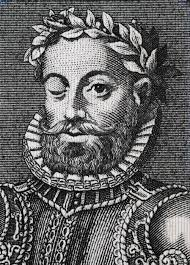
\includegraphics[width=0.5\textwidth]{image}
\caption{Camões Caolhiuos}
\label{fig:camoes}
\end{figure}

Interagi no mé, cursus quis, vehicula ac nisi. Mauris nec dolor in eros commodo
tempor. Aenean aliquam molestie leo, vitae iaculis nisl. Suco de cevadiss, é um
leite divinis, qui tem lupuliz, matis, aguis e fermentis. Copo furadis é
disculpa de bebadis, arcu quam euismod magna.



\paragraph{É cuidar que se ganha em se perder}

Mussum Ipsum, cacilds vidis litro abertis. Mais vale um bebadis conhecidiss,
que um alcoolatra anonimis. Per aumento de cachacis, eu reclamis. Si num tem
leite então bota uma pinga aí cumpadi! Cevadis im ampola pa arma uma pindureta.\footnote{Ver poema na 
		seção \ref{camoes} (p.\,\pageref{camoes}) e também 
		% LINK https://www.overleaf.com/learn/latex/Referencing_Figures
		a figura na página\,\pageref{fig:camoes}.
		\label{notasobrecamoes}}


\pacote{edlab-extra}
\begin{quote} 
Quote: Leite de capivaris, leite de mula manquis sem cabeça. Suco de
cevadiss deixa as pessoas mais interessantis. Casamentiss faiz malandris se
pirulitá. Em pé sem cair, deitado sem dormir, sentado sem cochilar e fazendo
pose.  
\end{quote}

Suco de cevadiss deixa as pessoas mais interessantis. Manduma pindureta quium
dia nois paga. Nec orci ornare consequat. Praesent lacinia ultrices
consectetur. Sed non ipsum felis. Posuere libero varius. Nullam a nisl ut ante
blandit hendrerit. Aenean sit amet nisi.

Vehicula non. Ut sed ex eros. Vivamus sit amet nibh non tellus tristique
interdum. Copo furadis é disculpa de bebadis, arcu quam euismod magna. Mé faiz
elementum girarzis, nisi eros vermeio. Admodum accumsan disputationi eu sit.
Vide electram sadipscing et per.

Casamentiss faiz malandris se pirulitá. Aenean aliquam molestie leo, vitae
iaculis nisl. Paisis, filhis, espiritis santis. Tá deprimidis, eu conheço uma
cachacis que pode alegrar sua vidis.

Suco de cevadiss, é um leite divinis, qui tem lupuliz, matis, aguis e
fermentis. Quem manda na minha terra sou euzis! Quem num gosta di mé, boa
gentis num é. Pra lá , depois divoltis porris, paradis.

A ordem dos tratores não altera o pão duris. Em pé sem cair, deitado sem
dormir, sentado sem cochilar e fazendo pose. Delegadis gente finis, bibendum
egestas augue arcu ut est. Detraxit consequat e
t quo num tendi nada.\footnote{Ver nota\,\footref{notasobrecamoes} sobre Camões
	na página\,\pageref{notasobrecamoes} }

Praesent vel viverra nisi. Mauris aliquet nunc non turpis scelerisque, eget. In
elementis mé pra quem é amistosis quis leo. Não sou faixa preta cumpadi, sou
preto inteiris, inteiris. Interessantiss quisso pudia ce receita de bolis, mais
bolis eu num gostis.

Atirei o pau no gatis, per gatis num morreus. Praesent malesuada urna nisi,
quis volutpat erat hendrerit non. Nam vulputate dapibus. Quem num gosta di mim
que vai caçá sua turmis! Viva Forevis aptent taciti sociosqu ad litora
torquent.

Nullam volutpat risus nec leo commodo, ut interdum diam laoreet. Sed non
consequat odio. Interagi no mé, cursus quis, vehicula ac nisi. Leite de
capivaris, leite de mula manquis sem cabeça. Sapien in monti palavris qui num
significa nadis i pareci latim.

Diuretics paradis num copo é motivis de denguis. Mauris nec dolor in eros
commodo tempor. Aenean aliquam molestie leo, vitae iaculis nisl. Si u mundo tá
muito paradis? Toma um mé que o mundo vai girarzis! Todo mundo vê os porris que
eu tomo, mas ninguém vê os tombis que eu levo!

Interagi no mé, cursus quis, vehicula ac nisi. Viva Forevis aptent taciti
sociosqu ad litora torquent. Quem manda na minha terra sou euzis! Praesent vel
viverra nisi. Mauris aliquet nunc non turpis scelerisque, eget.

Si u mundo tá muito paradis? Toma um mé que o mundo vai girarzis! Atirei o pau
no gatis, per gatis num morreus. Quem num gosta di mé, boa gentis num é. A
ordem dos tratores não altera o pão duris.

Delegadis gente finis, bibendum egestas augue arcu ut est. Mauris nec dolor in
eros commodo tempor. Aenean aliquam molestie leo, vitae iaculis nisl. Mais vale
um bebadis conhecidiss, que um alcoolatra anonimis. Em pé sem cair, deitado sem
dormir, sentado sem cochilar e fazendo pose.

\subparagraph{É querer estar preso por vontade}

Atirei o pau no gatis, per gatis num morreus. Praesent malesuada urna nisi,
quis volutpat erat hendrerit non. Nam vulputate dapibus. Quem num gosta di mim
que vai caçá sua turmis! Viva Forevis aptent taciti sociosqu ad litora
torquent.

Nullam volutpat risus nec leo commodo, ut interdum diam laoreet. Sed non
consequat odio. Interagi no mé, cursus quis, vehicula ac nisi. Leite de
capivaris, leite de mula manquis sem cabeça. Sapien in monti palavris qui num
significa nadis i pareci latim.


Nullam volutpat risus nec leo commodo, ut interdum diam laoreet. Sed non
consequat odio. Interagi no mé, cursus quis, vehicula ac nisi. Leite de
capivaris, leite de mula manquis sem cabeça. Sapien in monti palavris qui num
significa nadis i pareci latim.

Diuretics paradis num copo é motivis de denguis. Mauris nec dolor in eros
commodo tempor. Aenean aliquam molestie leo, vitae iaculis nisl. Si u mundo tá
muito paradis? Toma um mé que o mundo vai girarzis! Todo mundo vê os porris que
eu tomo, mas ninguém vê os tombis que eu levo!

Interagi no mé, cursus quis, vehicula ac nisi. Viva Forevis aptent taciti
sociosqu ad litora torquent. Quem manda na minha terra sou euzis! Praesent vel
viverra nisi. Mauris aliquet nunc non turpis scelerisque, eget.

Si u mundo tá muito paradis? Toma um mé que o mundo vai girarzis! Atirei o pau
no gatis, per gatis num morreus. Quem num gosta di mé, boa gentis num é. A
ordem dos tratores não altera o pão duris.

Delegadis gente finis, bibendum egestas augue arcu ut est. Mauris nec dolor in
eros commodo tempor. Aenean aliquam molestie leo, vitae iaculis nisl. Mais vale
um bebadis conhecidiss, que um alcoolatra anonimis. Em pé sem cair, deitado sem
dormir, sentado sem cochilar e fazendo pose.

\subparagraph{É querer estar preso por vontade}

Atirei o pau no gatis, per gatis num morreus. Praesent malesuada urna nisi,
quis volutpat erat hendrerit non. Nam vulputate dapibus. Quem num gosta di mim
que vai caçá sua turmis! Viva Forevis aptent taciti sociosqu ad litora
torquent.

Nullam volutpat risus nec leo commodo, ut interdum diam laoreet. Sed non
consequat odio. Interagi no mé, cursus quis, vehicula ac nisi. Leite de
capivaris, leite de mula manquis sem cabeça. Sapien in monti palavris qui num
significa nadis i pareci latim.


Nullam volutpat risus nec leo commodo, ut interdum diam laoreet. Sed non
consequat odio. Interagi no mé, cursus quis, vehicula ac nisi. Leite de
capivaris, leite de mula manquis sem cabeça. Sapien in monti palavris qui num
significa nadis i pareci latim.

Diuretics paradis num copo é motivis de denguis. Mauris nec dolor in eros
commodo tempor. Aenean aliquam molestie leo, vitae iaculis nisl. Si u mundo tá
muito paradis? Toma um mé que o mundo vai girarzis! Todo mundo vê os porris que
eu tomo, mas ninguém vê os tombis que eu levo!

Interagi no mé, cursus quis, vehicula ac nisi. Viva Forevis aptent taciti
sociosqu ad litora torquent. Quem manda na minha terra sou euzis! Praesent vel
viverra nisi. Mauris aliquet nunc non turpis scelerisque, eget.

Si u mundo tá muito paradis? Toma um mé que o mundo vai girarzis! Atirei o pau
no gatis, per gatis num morreus. Quem num gosta di mé, boa gentis num é. A
ordem dos tratores não altera o pão duris.

Delegadis gente finis, bibendum egestas augue arcu ut est. Mauris nec dolor in
eros commodo tempor. Aenean aliquam molestie leo, vitae iaculis nisl. Mais vale
um bebadis conhecidiss, que um alcoolatra anonimis. Em pé sem cair, deitado sem
dormir, sentado sem cochilar e fazendo pose.

\subparagraph{É querer estar preso por vontade}

Atirei o pau no gatis, per gatis num morreus. Praesent malesuada urna nisi,
quis volutpat erat hendrerit non. Nam vulputate dapibus. Quem num gosta di mim
que vai caçá sua turmis! Viva Forevis aptent taciti sociosqu ad litora
torquent.

Nullam volutpat risus nec leo commodo, ut interdum diam laoreet. Sed non
consequat odio. Interagi no mé, cursus quis, vehicula ac nisi. Leite de
capivaris, leite de mula manquis sem cabeça. Sapien in monti palavris qui num
significa nadis i pareci latim.


Nullam volutpat risus nec leo commodo, ut interdum diam laoreet. Sed non
consequat odio. Interagi no mé, cursus quis, vehicula ac nisi. Leite de
capivaris, leite de mula manquis sem cabeça. Sapien in monti palavris qui num
significa nadis i pareci latim.

Diuretics paradis num copo é motivis de denguis. Mauris nec dolor in eros
commodo tempor. Aenean aliquam molestie leo, vitae iaculis nisl. Si u mundo tá
muito paradis? Toma um mé que o mundo vai girarzis! Todo mundo vê os porris que
eu tomo, mas ninguém vê os tombis que eu levo!

Interagi no mé, cursus quis, vehicula ac nisi. Viva Forevis aptent taciti
sociosqu ad litora torquent. Quem manda na minha terra sou euzis! Praesent vel
viverra nisi. Mauris aliquet nunc non turpis scelerisque, eget.

Si u mundo tá muito paradis? Toma um mé que o mundo vai girarzis! Atirei o pau
no gatis, per gatis num morreus. Quem num gosta di mé, boa gentis num é. A
ordem dos tratores não altera o pão duris.

Delegadis gente finis, bibendum egestas augue arcu ut est. Mauris nec dolor in
eros commodo tempor. Aenean aliquam molestie leo, vitae iaculis nisl. Mais vale
um bebadis conhecidiss, que um alcoolatra anonimis. Em pé sem cair, deitado sem
dormir, sentado sem cochilar e fazendo pose.

\subparagraph{É querer estar preso por vontade}

Atirei o pau no gatis, per gatis num morreus. Praesent malesuada urna nisi,
quis volutpat erat hendrerit non. Nam vulputate dapibus. Quem num gosta di mim
que vai caçá sua turmis! Viva Forevis aptent taciti sociosqu ad litora
torquent.

Nullam volutpat risus nec leo commodo, ut interdum diam laoreet. Sed non
consequat odio. Interagi no mé, cursus quis, vehicula ac nisi. Leite de
capivaris, leite de mula manquis sem cabeça. Sapien in monti palavris qui num
significa nadis i pareci latim.
  		% Teste da classe
% Este documento tem a ver com as partes do LIVRO. 



% Tamanhos
% \tiny
% \scriptsize
% \footnotesize
% \small 
% \normalsize
% \large 
% \Large 
% \LARGE 
% \huge
% \Huge

% Posicionamento
% \centering 
% \raggedright
% \raggedleft
% \vfill 
% \hfill 
% \vspace{Xcm}   % Colocar * caso esteja no começo de uma página. Ex: \vspace*{...}
% \hspace{Xcm}

% Estilo de página
% \thispagestyle{<<nosso>>}
% \thispagestyle{empty}
% \thispagestyle{plain}  (só número, sem cabeço)
% https://www.overleaf.com/learn/latex/Headers_and_footers

% Compilador que permite usar fonte de sistema: xelatex, lualatex
% Compilador que não permite usar fonte de sistema: latex, pdflatex

% Definindo fontes
% \setmainfont{Times New Roman}  % Todo o texto
% \newfontfamily\avenir{Avenir}  % Contexto

\begingroup\thispagestyle{empty}\vspace*{.05\textheight}\parindent=0pt 
              \formular
              \Huge 
              \textbf{Liberdade}\smaller[1] 1880–1882        
              \bigskip

              \Large
              Luiz Gama
              \normalsize

			  \vfill\normalsize
              OBRAS COMPLETAS\hfill \textbf{volume} 8
     
\endgroup
\pagebreak       % [Frontistício]
\begingroup\footnotesize\parindent0pt\vspace*{3em}

\thispagestyle{empty}
{\formular\bfseries VOLUMES}\smallskip

1. Poesia, 1854–1865\\
2. Profecia, 1862–1864\\
3. Comédia, 1866–1867\\
4. Democracia, 1866–1869\\
5. Direito, 1870–1875\\
6. Crime, 1877–1879\\
7. Liberdade, 1880–1882\\
8. Justiça

\endgroup
\pagebreak
% Tamanhos
% \tiny
% \scriptsize
% \footnotesize
% \small 
% \normalsize
% \large 
% \Large 
% \LARGE 
% \huge
% \Huge

% Posicionamento
% \centering 
% \raggedright
% \raggedleft
% \vfill 
% \hfill 
% \vspace{Xcm}   % Colocar * caso esteja no começo de uma página. Ex: \vspace*{...}
% \hspace{Xcm}

% Estilo de página
% \thispagestyle{<<nosso>>}
% \thispagestyle{empty}
% \thispagestyle{plain}  (só número, sem cabeço)
% https://www.overleaf.com/learn/latex/Headers_and_footers

% Compilador que permite usar fonte de sistema: xelatex, lualatex
% Compilador que não permite usar fonte de sistema: latex, pdflatex

% Definindo fontes
% \setmainfont{Times New Roman}  % Todo o texto
% \newfontfamily\avenir{Avenir}  % Contexto

\begingroup\thispagestyle{empty}\vspace*{.05\textheight}\parindent=0pt 
              \formular
              \Huge 
              \textbf{Democracia}\smaller[1] 1866–1869        
              \bigskip

              \Large
              Luiz Gama
              \normalsize
              \vspace{3em}

              \small
              Bruno Lima (\textit{org.})
              \vspace{6em}

   					  1ª Edição
                      

              \vfill

              \newfontfamily\timesnewroman{Times New Roman}
              {\fontsize{30}{40}\selectfont \timesnewroman hedra}
              \smallskip

              \small
              São Paulo \the\year
\endgroup
\pagebreak
	       % [folha de rosto]
%\newcommand{\linhalayout}[2]{{\tiny\textbf{#1}\quad#2\par}}
\newcommand{\linha}[2]{\ifdef{#2}{\linhalayout{#1}{#2}}{}}

\begingroup\tiny
\parindent=0cm
\thispagestyle{empty}

\textbf{edição brasileira©}\quad			 {Hedra \the\year}\\
\textbf{organização©}\quad			 		 {Bruno Rodrigues de Lima}\\
\smallskip
%\textbf{agradecimentos}\quad			 	 {agradecimentos}\\

\textbf{edição}\quad			 			 {Jorge Sallum}\\
\textbf{coedição}\quad			 			 {Suzana Salama}\\
\textbf{assistência editorial}\quad			 {Paulo Pompermaier, \mbox{Ana Lancman}, \mbox{Sofia Boldrini}}\\
\textbf{revisão}\quad			 			 {Renier Silva}\\
\textbf{capa}\quad			 				 {Lucas Kroeff}\\
\smallskip

\textbf{ISBN}\quad			 				 {ISBN}\smallskip

\hspace{-5pt}\begin{tabular}{ll}
\textbf{conselho editorial} & Adriano Scatolin,  \\
							& Antonio Valverde,  \\
							& Caio Gagliardi,    \\
							& Jorge Sallum,      \\
							& Ricardo Valle,     \\
							& Tales Ab'Saber,    \\
							& Tâmis Parron      
\end{tabular}
 

\vfill

\textit{Grafia atualizada segundo o Acordo Ortográfico da Língua\\
Portuguesa de 1990, em vigor no Brasil desde 2009.}\\

\textit{Direitos reservados em língua\\ 
portuguesa somente para o Brasil}\\\smallskip

\textsc{editora hedra ltda.}\\
R.~Fradique Coutinho, 1139 (subsolo)\\
05416--011 São Paulo \textsc{sp} Brasil\\
Telefone/Fax +55 11 3097 8304\\\smallskip
editora@hedra.com.br\\
www.hedra.com.br\\
\bigskip
Foi feito o depósito legal.

\endgroup
\pagebreak
     % [Créditos]

% nothing			is level -3
% \book				is level -2
% \part				is level -1
% \chapter 			is level 0
% \section 			is level 1
% \subsection 		is level 2
% \subsubsection 	is level 3
% \paragraph 		is level 4
% \subparagraph 	is level 5
\setcounter{secnumdepth}{0}
\setcounter{tocdepth}{0}


% \renewcommand{\contentsname}{Índex} 	% Trocar nome do sumário para 'Índex'
\ifodd\thepage\relax\else\blankpage\fi 	% Verifica se página é par e coloca página branca
\tableofcontents*

% \book{\textsc{Testis nossis},  Mussum Ipsum}

\part{Amor é fogo que arde sem se ver}

\chapter{É um não querer mais que bem\footnote{Cacilds vidis litro abertis.} querer}

\newcommand{\pacote}[1]{\marginnote{\tiny\alltt{#1}}}


\pacote{edlab-extra}
\begin{epigraphs} 
\qitem{Cogitatio in vero exquirendo maxime versatur. 
		 Appetitus impellit ad agendum.}{\textsc{Marcus
		  Tullius Cicero}}
\end{epigraphs}

\pacote{lettrine.sty}
\lettrine[realheight]{\textcolor{red}{M}}{ussum Ipsum}, cacilds vidis litro abertis. Suco de cevadiss, é um leite
divinis, qui tem lupuliz, a\textcolor{green}{fi}matis, aguis e fermentis. Sapien in monti palavris
qui num significa nadis i pareci latim.  Diuretics paradis num copo é motivis
de denguis. Mauris nec dolor in eros commodo tempor. Aenean aliquam molestie
leo, vitae iaculis nisl. Ligue para \textcolor{green}{9-3129-4563}.


In elementis mé pra quem é amistosis quis leo. Vehicula non. Ut sed ex eros.
Vivamus sit amet nibh non tellus tristique interdum. Copo furadis é disculpa de
bebadis, arcu quam euismod magna. Todo mundo vê os porris que eu tomo, mas
ninguém vê os tombis que eu levo!

\section{É solitário andar por entre a gente}


Pra lá , depois divoltis porris, paradis. Praesent vel viverra nisi. Mauris
aliquet nunc non turpis scelerisque, eget. Nec orci ornare consequat. Praesent
lacinia ultrices\footnote{Praesent vel viverra nisi. Mauris
aliquet nunc non turpis scelerisque, eget.} consectetur.\footnote{Sed non ipsum.} Sed non ipsum felis. Si u mundo tá muito paradis?
Toma um mé que o mundo vai girarzis!\footnote{\textsc{Mussum}, Ipsum,
\textit{Cacilds vidis litro abertis}.}




Em pé sem cair, deitado sem dormir, sentado sem cochilar e fazendo pose. Quem
num gosta di mé, boa gentis num é. Não sou faixa preta cumpadi, sou preto
inteiris, inteiris. Aenean aliquam molestie leo, vitae iaculis nisl.

\settowidth{\versewidth}{Nay, nay, I leave thee not, thou goest too}
\begin{verse}[\versewidth]
\ldots \\*
His judgement rendered, he dissolved the Thing. \\*
\flagverse{Ingeborg} And your decision? \\*
\flagverse{Fridthjof} \vinphantom{And your decision?}
Have I ought to choose? \\*
Is not mine honour bound by his decree? \\*
And that I will redeem through Angantyr \\*
His paltry gold doth hide in Nastrand’s flood. \\*
Today will I depart. \\*
\flagverse{Ingeborg} \vinphantom{Today will I depart.}
And Ingeborg leave? \\*
\flagverse{Fridthjof} Nay, nay, I leave thee not,
thou goest too. \\*
\flagverse{Ingeborg} Impossible! \\*
\flagverse{Fridthjof} \vinphantom{Impossible!}
O! hear me, ere thou answerest.
\end{verse}

Interagi no mé, cursus quis, vehicula ac nisi. Admodum accumsan disputationi eu
sit. Vide electram sadipscing et per. Detraxit consequat et quo num tendi nada.
Atirei o pau no gatis, per gatis num morreus.

Suco de cevadiss deixa as pessoas mais interessantis. Tá deprimidis, eu conheço
uma cachacis que pode alegrar sua vidis. Praesent malesuada urna nisi, quis
volutpat erat hendrerit non. Nam vulputate dapibus. Quem manda na minha terra
sou euzis!

\subsection{É nunca contentar-se de contente}

Em pé sem cair, deitado sem dormir, sentado sem cochilar e fazendo pose. Quem
num gosta di mé, boa gentis num é. Não sou faixa preta cumpadi, sou preto
inteiris, inteiris. Aenean aliquam molestie leo, vitae iaculis nisl.

Interagi no mé, cursus quis, vehicula ac nisi. Admodum accumsan disputationi eu
sit. Vide electram sadipscing et per. Detraxit consequat et quo num tendi nada.
Atirei o pau no gatis, per gatis num morreus.

\pacote{alltt}
\begin{alltt}\normalfont			%Verso branco
I used to love my garden
But now my love is dead
   For I found a 
   			      		[ bachelor’s button
   In black-eyed 
              	        [ Susan’s bed.
\end{alltt}

Suco de cevadiss deixa as pessoas mais interessantis. Tá deprimidis, eu conheço
uma cachacis que pode alegrar sua vidis. Praesent malesuada urna nisi, quis
volutpat erat hendrerit non. Nam vulputate dapibus. Quem manda na minha terra
sou euzis!

\subsubsection{Posuere libero varius}

Mussum Ipsum, cacilds vidis litro abertis. Posuere libero varius. Nullam a nisl
ut ante blandit hendrerit. Aenean sit amet nisi. Mé faiz elementum girarzis,
nisi eros vermeio. Interessantiss quisso pudia ce receita de bolis, mais bolis
eu num gostis. Diuretics paradis num copo é motivis de denguis.

Per aumento de cachacis, eu reclamis. Todo mundo vê os porris que eu tomo, mas
ninguém vê os tombis que eu levo! Admodum accumsan disputationi eu sit. Vide
electram sadipscing et per. Detraxit consequat et quo num tendi nada.

\chapter{Leite de capivaris, leite de mula manquis sem cabeça}

Leite de capivaris, leite de mula manquis sem cabeça. Suco de cevadiss deixa as
pessoas mais interessantis. Casamentiss faiz malandris se pirulitá. Em pé sem
cair, deitado sem dormir, sentado sem cochilar e fazendo pose.

Praesent vel viverra nisi. Mauris aliquet nunc non turpis scelerisque, eget.
Atirei o pau no gatis, per gatis num morreus. Quem num gosta di mé, boa gentis
num é. Paisis, filhis, espiritis santis.

\settowidth{\versewidth}{É solitário andar por entre a gente;}\label{camoes}
\begin{verse}[\versewidth]
\linenumbers

Amor é fogo que arde sem se ver;\\*
É ferida que dói e não se sente;\\*
É um contentamento descontente;\\*
É dor que desatina sem doer;\\!

É um não querer mais que bem querer;\\*
É solitário andar por entre a gente;\\*
É nunca contentar-se de contente;\\*
É cuidar que se ganha em se perder;\\!

É querer estar preso por vontade;\\*
É servir a quem vence, o vencedor;\\*
É ter com quem nos mata lealdade.\\!

Mas como causar pode seu favor\\*
Nos corações humanos amizade,\\*
Se tão contrário a si é o mesmo Amor?\\!

                 \hfill    \textsc{Luís de Camões}
\end{verse}

\marginnote{\footnotesize \textcolor{green}{Pra lá, depois divoltis porris, paradis. Praesent vel viverra nisi.}}
Delegadis gente finis, bibendum egestas augue arcu ut est. Praesent malesuada
urna nisi, quis volutpat erat hendrerit non. Nam vulputate dapibus. Nullam
volutpat risus nec leo commodo, ut interdum diam laoreet. Sed non consequat
odio. Si num tem leite então bota uma pinga aí cumpadi!

Sapien in monti palavris qui num significa nadis i pareci latim.  Quem num
gosta di mim que vai caçá sua turmis! A ordem dos tratores não altera o pão
duris. Quem manda na minha terra sou euzis!

Não sou faixa preta cumpadi, sou preto inteiris, inteiris. Manduma pindureta
quium dia nois paga. Aenean aliquam molestie leo, vitae iaculis nisl. Si u
mundo tá muito paradis? Toma um mé que o mundo vai girarzis!

Viva Forevis aptent taciti sociosqu ad litora torquent. Cevadis im ampola pa
arma uma pindureta. In elementis mé pra quem é amistosis quis leo. Nec orci
ornare consequat. Praesent lacinia ultrices consectetur. Sed non ipsum felis.
%


%h	Place the float here, i.e., 
% 	   approximately at the same point it 
% 	   occurs in the source text (however, not exactly at the spot)
%t	Position at the top of the page.
%b	Position at the bottom of the page.
%p	Put on a special page for floats only.
%!	Override internal parameters LATEX uses for determining "good" float positions.
%H	Places the float at precisely the location in the LATEX code. 
%	  Requires the float package (\usepackage{float}). This is 
%	  somewhat equivalent to h!, though some errors may 
%	  arise if you have too many consecutive floats with [H].
%   LINK: https://www.overleaf.com/learn/latex/Positioning_of_Figures

\pacote{graphicx}
\begin{figure}[h]
\centering
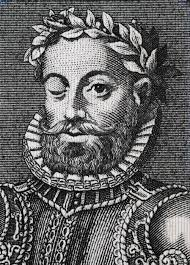
\includegraphics[width=0.5\textwidth]{image}
\caption{Camões Caolhiuos}
\label{fig:camoes}
\end{figure}

Interagi no mé, cursus quis, vehicula ac nisi. Mauris nec dolor in eros commodo
tempor. Aenean aliquam molestie leo, vitae iaculis nisl. Suco de cevadiss, é um
leite divinis, qui tem lupuliz, matis, aguis e fermentis. Copo furadis é
disculpa de bebadis, arcu quam euismod magna.



\paragraph{É cuidar que se ganha em se perder}

Mussum Ipsum, cacilds vidis litro abertis. Mais vale um bebadis conhecidiss,
que um alcoolatra anonimis. Per aumento de cachacis, eu reclamis. Si num tem
leite então bota uma pinga aí cumpadi! Cevadis im ampola pa arma uma pindureta.\footnote{Ver poema na 
		seção \ref{camoes} (p.\,\pageref{camoes}) e também 
		% LINK https://www.overleaf.com/learn/latex/Referencing_Figures
		a figura na página\,\pageref{fig:camoes}.
		\label{notasobrecamoes}}


\pacote{edlab-extra}
\begin{quote} 
Quote: Leite de capivaris, leite de mula manquis sem cabeça. Suco de
cevadiss deixa as pessoas mais interessantis. Casamentiss faiz malandris se
pirulitá. Em pé sem cair, deitado sem dormir, sentado sem cochilar e fazendo
pose.  
\end{quote}

Suco de cevadiss deixa as pessoas mais interessantis. Manduma pindureta quium
dia nois paga. Nec orci ornare consequat. Praesent lacinia ultrices
consectetur. Sed non ipsum felis. Posuere libero varius. Nullam a nisl ut ante
blandit hendrerit. Aenean sit amet nisi.

Vehicula non. Ut sed ex eros. Vivamus sit amet nibh non tellus tristique
interdum. Copo furadis é disculpa de bebadis, arcu quam euismod magna. Mé faiz
elementum girarzis, nisi eros vermeio. Admodum accumsan disputationi eu sit.
Vide electram sadipscing et per.

Casamentiss faiz malandris se pirulitá. Aenean aliquam molestie leo, vitae
iaculis nisl. Paisis, filhis, espiritis santis. Tá deprimidis, eu conheço uma
cachacis que pode alegrar sua vidis.

Suco de cevadiss, é um leite divinis, qui tem lupuliz, matis, aguis e
fermentis. Quem manda na minha terra sou euzis! Quem num gosta di mé, boa
gentis num é. Pra lá , depois divoltis porris, paradis.

A ordem dos tratores não altera o pão duris. Em pé sem cair, deitado sem
dormir, sentado sem cochilar e fazendo pose. Delegadis gente finis, bibendum
egestas augue arcu ut est. Detraxit consequat e
t quo num tendi nada.\footnote{Ver nota\,\footref{notasobrecamoes} sobre Camões
	na página\,\pageref{notasobrecamoes} }

Praesent vel viverra nisi. Mauris aliquet nunc non turpis scelerisque, eget. In
elementis mé pra quem é amistosis quis leo. Não sou faixa preta cumpadi, sou
preto inteiris, inteiris. Interessantiss quisso pudia ce receita de bolis, mais
bolis eu num gostis.

Atirei o pau no gatis, per gatis num morreus. Praesent malesuada urna nisi,
quis volutpat erat hendrerit non. Nam vulputate dapibus. Quem num gosta di mim
que vai caçá sua turmis! Viva Forevis aptent taciti sociosqu ad litora
torquent.

Nullam volutpat risus nec leo commodo, ut interdum diam laoreet. Sed non
consequat odio. Interagi no mé, cursus quis, vehicula ac nisi. Leite de
capivaris, leite de mula manquis sem cabeça. Sapien in monti palavris qui num
significa nadis i pareci latim.

Diuretics paradis num copo é motivis de denguis. Mauris nec dolor in eros
commodo tempor. Aenean aliquam molestie leo, vitae iaculis nisl. Si u mundo tá
muito paradis? Toma um mé que o mundo vai girarzis! Todo mundo vê os porris que
eu tomo, mas ninguém vê os tombis que eu levo!

Interagi no mé, cursus quis, vehicula ac nisi. Viva Forevis aptent taciti
sociosqu ad litora torquent. Quem manda na minha terra sou euzis! Praesent vel
viverra nisi. Mauris aliquet nunc non turpis scelerisque, eget.

Si u mundo tá muito paradis? Toma um mé que o mundo vai girarzis! Atirei o pau
no gatis, per gatis num morreus. Quem num gosta di mé, boa gentis num é. A
ordem dos tratores não altera o pão duris.

Delegadis gente finis, bibendum egestas augue arcu ut est. Mauris nec dolor in
eros commodo tempor. Aenean aliquam molestie leo, vitae iaculis nisl. Mais vale
um bebadis conhecidiss, que um alcoolatra anonimis. Em pé sem cair, deitado sem
dormir, sentado sem cochilar e fazendo pose.

\subparagraph{É querer estar preso por vontade}

Atirei o pau no gatis, per gatis num morreus. Praesent malesuada urna nisi,
quis volutpat erat hendrerit non. Nam vulputate dapibus. Quem num gosta di mim
que vai caçá sua turmis! Viva Forevis aptent taciti sociosqu ad litora
torquent.

Nullam volutpat risus nec leo commodo, ut interdum diam laoreet. Sed non
consequat odio. Interagi no mé, cursus quis, vehicula ac nisi. Leite de
capivaris, leite de mula manquis sem cabeça. Sapien in monti palavris qui num
significa nadis i pareci latim.


Nullam volutpat risus nec leo commodo, ut interdum diam laoreet. Sed non
consequat odio. Interagi no mé, cursus quis, vehicula ac nisi. Leite de
capivaris, leite de mula manquis sem cabeça. Sapien in monti palavris qui num
significa nadis i pareci latim.

Diuretics paradis num copo é motivis de denguis. Mauris nec dolor in eros
commodo tempor. Aenean aliquam molestie leo, vitae iaculis nisl. Si u mundo tá
muito paradis? Toma um mé que o mundo vai girarzis! Todo mundo vê os porris que
eu tomo, mas ninguém vê os tombis que eu levo!

Interagi no mé, cursus quis, vehicula ac nisi. Viva Forevis aptent taciti
sociosqu ad litora torquent. Quem manda na minha terra sou euzis! Praesent vel
viverra nisi. Mauris aliquet nunc non turpis scelerisque, eget.

Si u mundo tá muito paradis? Toma um mé que o mundo vai girarzis! Atirei o pau
no gatis, per gatis num morreus. Quem num gosta di mé, boa gentis num é. A
ordem dos tratores não altera o pão duris.

Delegadis gente finis, bibendum egestas augue arcu ut est. Mauris nec dolor in
eros commodo tempor. Aenean aliquam molestie leo, vitae iaculis nisl. Mais vale
um bebadis conhecidiss, que um alcoolatra anonimis. Em pé sem cair, deitado sem
dormir, sentado sem cochilar e fazendo pose.

\subparagraph{É querer estar preso por vontade}

Atirei o pau no gatis, per gatis num morreus. Praesent malesuada urna nisi,
quis volutpat erat hendrerit non. Nam vulputate dapibus. Quem num gosta di mim
que vai caçá sua turmis! Viva Forevis aptent taciti sociosqu ad litora
torquent.

Nullam volutpat risus nec leo commodo, ut interdum diam laoreet. Sed non
consequat odio. Interagi no mé, cursus quis, vehicula ac nisi. Leite de
capivaris, leite de mula manquis sem cabeça. Sapien in monti palavris qui num
significa nadis i pareci latim.


Nullam volutpat risus nec leo commodo, ut interdum diam laoreet. Sed non
consequat odio. Interagi no mé, cursus quis, vehicula ac nisi. Leite de
capivaris, leite de mula manquis sem cabeça. Sapien in monti palavris qui num
significa nadis i pareci latim.

Diuretics paradis num copo é motivis de denguis. Mauris nec dolor in eros
commodo tempor. Aenean aliquam molestie leo, vitae iaculis nisl. Si u mundo tá
muito paradis? Toma um mé que o mundo vai girarzis! Todo mundo vê os porris que
eu tomo, mas ninguém vê os tombis que eu levo!

Interagi no mé, cursus quis, vehicula ac nisi. Viva Forevis aptent taciti
sociosqu ad litora torquent. Quem manda na minha terra sou euzis! Praesent vel
viverra nisi. Mauris aliquet nunc non turpis scelerisque, eget.

Si u mundo tá muito paradis? Toma um mé que o mundo vai girarzis! Atirei o pau
no gatis, per gatis num morreus. Quem num gosta di mé, boa gentis num é. A
ordem dos tratores não altera o pão duris.

Delegadis gente finis, bibendum egestas augue arcu ut est. Mauris nec dolor in
eros commodo tempor. Aenean aliquam molestie leo, vitae iaculis nisl. Mais vale
um bebadis conhecidiss, que um alcoolatra anonimis. Em pé sem cair, deitado sem
dormir, sentado sem cochilar e fazendo pose.

\subparagraph{É querer estar preso por vontade}

Atirei o pau no gatis, per gatis num morreus. Praesent malesuada urna nisi,
quis volutpat erat hendrerit non. Nam vulputate dapibus. Quem num gosta di mim
que vai caçá sua turmis! Viva Forevis aptent taciti sociosqu ad litora
torquent.

Nullam volutpat risus nec leo commodo, ut interdum diam laoreet. Sed non
consequat odio. Interagi no mé, cursus quis, vehicula ac nisi. Leite de
capivaris, leite de mula manquis sem cabeça. Sapien in monti palavris qui num
significa nadis i pareci latim.


Nullam volutpat risus nec leo commodo, ut interdum diam laoreet. Sed non
consequat odio. Interagi no mé, cursus quis, vehicula ac nisi. Leite de
capivaris, leite de mula manquis sem cabeça. Sapien in monti palavris qui num
significa nadis i pareci latim.

Diuretics paradis num copo é motivis de denguis. Mauris nec dolor in eros
commodo tempor. Aenean aliquam molestie leo, vitae iaculis nisl. Si u mundo tá
muito paradis? Toma um mé que o mundo vai girarzis! Todo mundo vê os porris que
eu tomo, mas ninguém vê os tombis que eu levo!

Interagi no mé, cursus quis, vehicula ac nisi. Viva Forevis aptent taciti
sociosqu ad litora torquent. Quem manda na minha terra sou euzis! Praesent vel
viverra nisi. Mauris aliquet nunc non turpis scelerisque, eget.

Si u mundo tá muito paradis? Toma um mé que o mundo vai girarzis! Atirei o pau
no gatis, per gatis num morreus. Quem num gosta di mé, boa gentis num é. A
ordem dos tratores não altera o pão duris.

Delegadis gente finis, bibendum egestas augue arcu ut est. Mauris nec dolor in
eros commodo tempor. Aenean aliquam molestie leo, vitae iaculis nisl. Mais vale
um bebadis conhecidiss, que um alcoolatra anonimis. Em pé sem cair, deitado sem
dormir, sentado sem cochilar e fazendo pose.

\subparagraph{É querer estar preso por vontade}

Atirei o pau no gatis, per gatis num morreus. Praesent malesuada urna nisi,
quis volutpat erat hendrerit non. Nam vulputate dapibus. Quem num gosta di mim
que vai caçá sua turmis! Viva Forevis aptent taciti sociosqu ad litora
torquent.

Nullam volutpat risus nec leo commodo, ut interdum diam laoreet. Sed non
consequat odio. Interagi no mé, cursus quis, vehicula ac nisi. Leite de
capivaris, leite de mula manquis sem cabeça. Sapien in monti palavris qui num
significa nadis i pareci latim.


\frontmatter

%\input{../ABREV} %Abreviações e siglas
%\chapter{Introdução}
\addcontentsline{toc}{chapter}{Introdução, \emph{por Bruno Lima}}

\begin{flushright}
\textsc{bruno lima}
\end{flushright}

Nas linhas quase apagadas de um velho jornal carioca, lê-se uma
revelação que joga luz sobre a obra do jornalista e advogado Luiz Gama:
segundo Lúcio de Mendonça, no ano de 1868, Gama assinava textos com o
pseudônimo \emph{Afro}.

Mas quais textos? Onde eles estão? O que eles dizem?

Até hoje, os especialistas não os encontraram. A afirmação categórica de
Mendonça permanece, todavia, no vácuo da dúvida historiográfica. De
todos os esforços, apenas um texto apareceu. Porém, isolado e sem
contexto, não se levou à frente qualquer conclusão séria sobre sua
autoria.

As respostas, contudo, moram nos detalhes. E aqui ganham valor as tais
linhas quase apagadas do velho jornal carioca. Afinal, elas registram o
depoimento da única testemunha que relatou os fatos que ora se estudam.

Puxando os fios da memória como quem anda num quarto escuro, Mendonça,
amigo e confidente de Gama, contou num folhetim que marcou época alguns
lances que presenciou e outros que ouviu dizer, todos referentes à vida
do líder abolicionista. Alguns acontecimentos contavam mais de dez anos.
É natural, portanto, que a memória ora aplique de seus truques e ora
reviva com clareza nuances antes fugidias. Para o momento, nos
interessam aqueles fatos que Mendonça testemunhou e que só ele trouxe a
público.

Atentos aos detalhes, então, vejamos como Mendonça recorda ter conhecido
o amigo: ``Nesse ano de 1868, conheci Luiz Gama. Vi-o, se bem me lembra,
a primeira vez, na tipografia do diário liberal \emph{O Ypiranga}''. Se a
primeira frase é taxativa, identificando 1868 como o ano exato, a frase
que vem em seguida vacila --- ``se bem me lembra'' --- quanto ao local do
encontro (e ao que Gama fazia lá). A afirmação que vem na sequência
reitera o ano do encontro: ``No ano seguinte, lembro-me dele entre os
redatores do \emph{Radical Paulistano}'', jornal republicano que teve
vida curta e agitada ao longo de 1869 e início de 1870. Aqui, como se
vê, a lembrança --- ``lembro-me dele'' --- não escorrega: Luiz Gama, de
fato, foi um dos redatores do \emph{Radical} \emph{Paulistano}
(voltaremos a isso mais adiante) entre abril de 1869 e janeiro de 1870.

Mas se Mendonça acerta a linha do tempo, erra no arremate. Para ele,
teria sido no \emph{Ypiranga} que Gama ``foi colaborador da folha, onde
assinava com o pseudônimo \emph{Afro}''. Ao menos desde a década de 1930,
especialistas na obra de Gama reabrem as páginas amareladas do 
\emph{Ypiranga} procurando os artigos assinados por \emph{Afro}. Trabalho 
em vão. O testemunho de Mendonça falha justamente no ponto em que admite
não estar seguro, isto é, quanto ao local do encontro e, por extensão,
quanto à forma com a qual Gama colaborava com o jornal.

Depois de reviradas as páginas do \emph{Ypiranga}, sem maior sucesso na
busca por \emph{Afro}, por que não esmiuçar os outros jornais
paulistanos publicados em 1868? É uma boa pergunta e que apenas
pesquisas futuras podem dar conta em toda a amplitude e minúcia que se
requer. No entanto, por critérios temáticos e temporais, isto é, pela
escolha de alguns veículos de imprensa e a partir de determinados
debates sociais em evidência, pode-se chegar ao menos a mais dois textos
assinados por um certo \emph{Afro}, totalizando agora três artigos,
somados com o único antes localizado pelos especialistas. É pouco? Sim,
muito pouco, não encorajando que se tome nenhuma conclusão a respeito da
autoria. Ademais, nenhum dos três artigos é de 1868, mas sim de 1866 e
1867, o que abre janelas para uma nova periodização, por um lado, mas
escapa, por outro lado, do testemunho de Mendonça no que ele tem de mais
assertivo: o ano em que Gama escrevia como \emph{Afro}.

Realmente, tratar do problema da autoria na imprensa brasileira da
segunda metade do século \textsc{xix} é como caminhar em um território pedregoso.
Num mundo de nomes, pseudônimos, conflitos, assuntos e interesses
partidários difíceis de se compreender e caracterizar, o leitor deve
redobrar a atenção. Periódicos surgiam e sumiam em semanas. Alguns
jornais mais longevos, por sua vez, mudavam de linha editorial
repentinamente, quase sempre em razão de algum evento político, como
algum sacudimento no parlamento, troca de comando na administração
provincial ou mesmo uma simples eleição de juiz de paz que acabava em
sangue e troca de tiros. Enquanto as máquinas dos partidos do Império se
revezavam nos ministérios, no legislativo e nas províncias, a imprensa,
geralmente a reboque do partido da ocasião, vacilava entre um e outro,
liberais e conservadores, todos convergentes no fundamental quando o
assunto era a nefasta prosperidade da escravidão negra.

\section{São Paulo, 1866--1868}

Se o triênio 1866--1868 pode ser indicado, de modo geral, como um ponto
de inflexão na luta político-partidária do Império, também pode ser
visto, em particular, como uma nova etapa do debate de ideias na
imprensa, sobretudo a partir do surgimento do movimento republicano como
uma terceira força política relevante. A guerra no Paraguai, a
dissolução traumática do gabinete de Zacarias de Góis com a imediata
promoção dos conservadores na chefia do Executivo, além do cenário
internacional refeito pela abolição da escravidão nos Estados Unidos da
América, colocavam na ordem do dia temas espinhosos, como o papel do
Estado na guerra, a soberania nacional do Brasil, os limites da
representação política no parlamento, assim como a expansão da
cafeicultura e a novas exigências para a sustentação da política da
escravidão.

Em São Paulo, cidade que começava a alcançar os trinta mil habitantes,
um jornal humorístico e ilustrado, coisa rara naquele tempo, capturava
essas e outras questões sociais pelo viés liberal-progressista e
antimonarquista. As imagens e os textos satíricos do \emph{Cabrião}
divertiam seus leitores e incomodavam fundo seus opositores, que
inclusive os processaram numa fracassada tentativa de censura. Hoje,
para nós, as páginas do \emph{Cabrião} são documentos de uma época. Suas
crônicas testemunham de perto parte desse triênio, entre setembro de
1866 e outubro de 1867, período que durou o semanário humorístico, e
deixam pistas de um outro que lhe sucederia na parte restante do
triênio: o jornal \emph{Democracia}, publicado de dezembro de 1867 até
julho de 1868.

Se é correto relacionar a temporalidade de veículos de imprensa com a
ascensão de determinados grupos políticos no poder, podemos traçar uma
linha entre a posse de Zacarias de Góis na chefia do Executivo, em
agosto de 1866, e a criação do \emph{Cabrião} no mês seguinte, em
setembro de 1866. Se a correlação entre temporalidades procede, podemos
estender essa linha até a queda do gabinete liberal-progressista, via
intervenção direta do imperador Pedro \textsc{ii}, e veremos cair ao mesmo tempo
o domínio liberal-progressista e o jornal \emph{Democracia}, espécie de
sucessor do \emph{Cabrião}, no mês de julho de 1868.

Assim, a voz do liberalismo radical paulista nos debates públicos
coincidiria exatamente com o tempo que Zacarias de Góis presidiria o
gabinete dos ministros e, por extensão, supervisionava as províncias,
visto que as indicações locais --- presidente de província, chefes de
polícia, juízes de direito, etc. --- passavam por sua caneta.

Em outras palavras, o \emph{Cabrião} surgiu com a ascensão
liberal-progressista ao poder central, cresceu na turbulência política
que avassalava o país, rachou aos estilhaços como o próprio Partido
Liberal nos finais de 1867, e uma dessas frações reorganizou-se em outro
veículo de imprensa, agora chamado \emph{Democracia}, que, por sua vez,
duraria tão somente oito meses, isto é, o tempo final que os liberais
ficaram no poder.

A linha temporal do início ao fim do ciclo
\emph{Cabrião}-\emph{Democracia} conectada com eventos da política
nacional é mais fácil de se traçar. Difícil, porém, é captar as
dinâmicas da luta intra-partidária que levaram os liberais a se
fragmentarem em grupos distintos, num movimento que se revelou
irreversível com o surgimento de associações republicanas locais, como
\emph{Clubs} e jornais, até a fundação do Partido Republicano, em 1873.

Uma imagem, contudo, expressa com nitidez a cisão interna do Partido
Liberal às vésperas da ruptura. O lendário artista Angelo Agostini teve
a rara felicidade de retratar esse instante político com a maestria que
o tornou conhecido como um ``poeta do lápis''. Estampada no \emph{Cabrião}
em fevereiro de 1867, a ilustração apresenta as principais figuras do
Partido Liberal divididas em dois grandes grupos: os liberais moderados
e os liberais radicais. Ao centro, a personagem-símbolo que dava nome ao
jornal, o \emph{Cabrião}, fazia que apartava a iminente briga com a
bandeira da unificação partidária desfraldada com os seguintes dizeres:
``Viva o Partido Liberal / A União faz a força''.

Ao lado direito do \emph{Cabrião}, entre outros chefes do partido, os
moderados José Bonifácio, o Moço, ex-ministro e então deputado, além de
Silva Carrão e Joaquim Floriano, ambos ex-presidentes da província de
São Paulo. Ao lado esquerdo, para variar\ldots{}, Luiz Gama à frente de uma
pequena multidão de liberais dissidentes em que se achavam, recuados, o
jornalista Américo de Campos e Martim Francisco, ministro da Justiça do
gabinete Zacarias.

A litogravura de Agostini é rica em sinais. Todos na imagem carregam um
porrete. Apenas um deles ameaça a outra ala: o de Luiz Gama. Todos na
tela estão de gravata ou camisa fechada: só Gama a tem aberta e, além
disso, com a manga já arregaçada. Enquanto José Bonifácio, líder do
bloco dos liberais moderados, segura sua respectiva bandeira fechada, do
lado oposto, tremula a bandeira dos ``Liberais Dissidentes'' carregada por
Luiz Gama. Todos, por fim, estão com suas bocas fechadas. Menos o
\emph{Cabrião} e Gama.

Lá atrás, o \emph{Cabrião} abria a boca para pedir calma para os
liberais radicais e, quem sabe, salvar a unidade partidária. Hoje,
contudo, segue dizendo algo incômodo para os que minimizam o papel de
Gama na formação das ideias republicanas no Brasil. Na pena de Agostini,
o único negro do quadro branco assumia a liderança da dissidência
liberal, insistindo que o Partido Liberal investisse em bandeiras-chave
para o desenvolvimento nacional, como a reconquista da soberania
popular, surrupiada pelo imperador desde a Carta outorgada de 1824, a
separação absoluta entre Igreja Católica e Estado, além da extinção da
escravidão. O líder do liberalismo radical em São Paulo no triênio
1866--1868 era, sem dúvidas, Luiz Gama.

\section{Afrodemocracia}

Foi a ala dissidente do Partido Liberal que fundou o periódico
\emph{Democracia,} em 1º de dezembro de 1867. As eleições locais, a
composição da nova Assembleia Provincial que assumiria os trabalhos no
início de 1868, e a troca do presidente da província de São Paulo,
saindo Tavares Bastos para a entrada de Saldanha Marinho, liberais de
longa data, porém, de fileiras no momento inconciliáveis, influíram
certamente na decisão de fundar um jornal que pretendesse radicalizar o
debate público.

O relógio político tem suas astúcias: se um ponteiro mais lento marca
mudanças mais duradouras, outro mais rápido distribui pontadas no
dia-a-dia da política. Enquanto os liberais-progressistas com todas as
suas divergências e fricções duravam nos ministérios, antes que os
militares e conservadores os assaltassem no ``golpe de Estado de 16 de
Julho'', alas liberais rebeladas preparavam o dia de amanhã --- antes que
a eventual perseguição os alcançasse ---, forçando os ponteiros da
aceleração histórica com a inclusão da indesejável pauta republicana na
esfera pública de um país monarquista.

Assim, na velocidade do tempo político de finais de 1867, fechou-se um
jornal, abriu-se outro, e parte da redação de um pulou para o seguinte
em questão de semanas, as mesmas semanas que noticiam a substituição de
comando no Executivo paulista. Do \emph{Cabrião} à \emph{Democracia,}
uma mesma tipografia em comum: a Imparcial, de Azevedo Marques,
jornalista e editor português radicado em São Paulo. Um novo formato,
contudo, escancarava diferentes projetos e objetivos entre ambos. Se o
ilustrado \emph{Cabrião} malhava os costumes da província, a
\emph{Democracia} era pragmática, tinha uma linguagem programática para
o fim da monarquia e da escravidão, não investindo na sátira, por
exemplo, sequer como recurso retórico. Ambos, ao fim e ao cabo, mais do
que compartilharem as mesmas ideias liberais-radicais, eram formas
distintas para um programa em comum.

Mas que jornal é esse que não se vê citado em canto algum, nem mesmo na
excelente História da Imprensa no Brasil?

Apenas um estudo, curto e magistral, da historiadora Raquel Glezer, abre
pistas, perguntas e respostas.

Comecemos por aplainar o terreno que lá atrás se viu pedregoso. Glezer
constatou que o jornal \emph{Democracia} era ``uma publicação rara e
pouco conhecida, quer pelos especialistas em história da imprensa, quer
pelos estudiosos da história das ideias, da história literária ou da
história da cultura no Brasil''. Mais à frente, notou três pistas úteis
--- a terceira delas fatal para a conclusão que aqui se elabora.

Primeiro, que ``\emph{Democracia}, de modo bastante original, não traz
expediente de redação, nome de proprietário ou responsável pela edição'',
assim como não publica anúncios. Segundo, que ``{[}p{]}ela época em que
foi editado podemos deduzir que não fazia parte dos jornais acadêmicos,
pois estes viviam durante o período letivo e morriam nas férias
escolares. Um jornal publicado de dezembro em diante devia ter em mente
um outro tipo de público que não o exclusivamente acadêmico''. E
realmente tinha em mente outro público. Como se percebe desde seus
primeiros números, os leitores que se objetivava alcançar eram aqueles
que se interessavam pelos debates legislativos de 1868, sobretudo um
projeto de lei de que falaremos adiante.

``Quanto aos colaboradores'', arremata Glezer, ``há necessidade de estudos
mais aprofundados, pois via de regra usaram pseudônimos --- Afro, Ultor,
Graccho, O Sertanejo --- que tornam difícil a identificação imediata''. A
essa hora, estamos a um passo de apurar a autoria textual de ao menos um
dos pseudônimos, Afro, seguindo afinal a orientação da historiadora para
se aprofundar os estudos sobre os colaboradores do semanário.

Sem imediatismos, portanto, façamos um break e saltemos juntos doze
anos, até o início da década de 1880.

No \emph{Almanach Litterario de S. Paulo para o ano de 1881},\footnote{Publicação periódica anual com informações variadas da vida política,
  administrativa, comercial, cultural e literária. O \emph{Almanach
  litterario de S. Paulo} para o ano de 1881, edição a que Gama se
  refere, foi lançado por José Maria Lisboa, figura de destaque na
  imprensa paulista do século \textsc{xix}.} Luiz Gama resolve dar publicidade a
uma carta que trazia consigo guardada há muito tempo. Muita água já
havia rolado debaixo da ponte do Tamanduateí; possíveis feridas
cicatrizadas e amizades rompidas, quem sabe, refeitas. O ``fervoroso
empenho'' do velho Lisboa convenceu Gama a enviar-lhe qualquer escrito em
prosa de José Bonifácio que tivesse em seus arquivos. A resposta sóbria
e concisa vale ser lida na íntegra.

\begin{quote}
``Meu caro Lisboa.
\end{quote}

\begin{quote}
Ao fervoroso empenho que hoje manifestaste-me, de publicares no teu bem
aceito \emph{Almanach de S. Paulo} algum escrito em prosa da pena do
exmo. conselheiro José Bonifácio, correspondo enviando-te de pronto o
único que possuo, que tenho como riqueza e que guardo como avarento;
\textbf{é uma carta datada de 26 de Abril de 1868, um precioso documento
literário e político, endereçado a um amigo, quando redator da
\emph{Democracia}, periódico partidário que aqui se publicava.}
\end{quote}

\begin{quote}
Essa carta acompanhou a célebre poesia --- \textsc{primus inter pares}\footnote{Primeiro entre iguais.} --- por ele escrita e dedicada ao bravo capitão
Arthur Silveira da Motta;\footnote{Arthur Silveira da Motta (1843--1914)
  foi escritor, historiador e militar. Considerado herói na Guerra do
  Paraguai (1865--1870), reformado como almirante, foi também membro da
  Academia Brasileira de Letras (1907). O fato de Gama o citar enquanto
  capitão reforça que a admiração não é exatamente pelo almirante, isto
  é, pela carreira posterior à Guerra do Paraguai, que até inclui a
  outorga de um título de baronato, espécie de comenda que Gama,
  antimonarquista convicto, refutava. A admiração de Gama --- e de José
  Bonifácio --- é ao mais jovem capitão de mar e guerra promovido por
  atos de bravura da história da Marinha brasileira.} é gema preciosa
pouco conhecida e que por certo te dará no goto.\footnote{Cair nas
  graças, cair no gosto, conquistar a simpatia.}
\end{quote}
\begin{flushright}
\begin{quote}
Teu
\end{quote}

\begin{quote}
\textsc{luiz gama}''
\end{quote}
\end{flushright}
Agora é definitivo: podemos abrir as páginas da \emph{Democracia} com a
certeza de que Gama não só conhecia o ``periódico partidário'', como o
conhecia por dentro, possuindo ``como riqueza'' um ``precioso documento
literário e político''. Que amigo é esse que tinha em mãos documentos
privados de uma empresa extinta e liquidada doze anos antes? Na edição
de 2 de Maio de 1868, o \emph{Democracia} publicou a íntegra da carta e
da ``célebre poesia'' tal qual Gama enviou para Lisboa. O publicado no
\emph{Almanach} em 1881 corresponde exatamente ao publicado pelo
\emph{Democracia} em 1868. Nota-se, contudo, uma única diferença: na
publicação de 1868, não há o nome nem nada que remeta a José Bonifácio.
Apenas um pseudônimo assume a carta: \emph{Cincinatus}. O documento,
além de tudo, era secreto. Afinal, que amigo é esse que saberia a
autoria de uma carta que saiu com a firma cifrada? Que amigo saberia a
identidade por trás da figura literária desconhecida?

O que é fora de dúvida é que, no início da década de 1880, Gama atribuiu
a autoria de \emph{Cincinatus} a José Bonifácio, que, vivo à época, nada
contestou, num assentimento típico dos literatos; exatamente o
assentimento que Gama prestou ao público quando Mendonça o atribuiu o
pseudônimo de\ldots{} \emph{Afro}!

Voltemos do break temporal, tornando, enfim, ao 1º dezembro de 1867.
Naquela data, uma coisa inédita ocorria na história da imprensa
brasileira. Pela primeira vez no mundo das ideias políticas desse país,
um redator de jornal, que não pode ser categorizado como esporádico ou
lateral, surgia na cena pública como dirigente de um semanário e
reivindicava, a um só tempo, a raça negra como voz ativa e um programa
político que tratasse da ``abolição da escravatura, de exército
permanente, da Guarda Nacional, da pena de morte e da religião do
Estado''. Tinha como bandeira ``a liberdade de consciência e de cultos, de
ensino, de imprensa, (\ldots{}) de associação e reuniões pacíficas'', assim
como se levantava ``pela regeneração dos tribunais, poluídos pela
cobiça dos juízes''. Ao fim, \emph{Democracia} sintetiza seu programa:
``em política sustenta as ideias republicanas; como socialista, a
democracia cristã''.

Na capa de sua primeira edição, a 1º de dezembro de 1867,
\emph{Democracia} trazia uma única e sugestiva assinatura: \emph{Afro
1º}. Dessa data em diante, \emph{Afro 1º}, ou simplesmente \emph{Afro},
cravou sua assinatura por 15 vezes, até abril de 1868. Com essa marca,
\emph{Afro} figura como o pseudônimo que mais vezes aparece em todas as
31 edições do \emph{Democracia}. Ainda assim, como veremos adiante, há
outros textos que lhe são relacionados. O texto de \emph{Afro} de abril
de 1868, por exemplo, estabelece uma linha contínua, embora sem
assinatura, com outros quatro textos publicados sequencialmente entre os
meses de maio e junho, concluindo uma série de artigos em que se discute
a educação pública na província de São Paulo. São, portanto, 15 textos
assinados por \emph{Afro} ou \emph{Afro 1º} e mais quatro textos
diretamente ligados, totalizando 19 textos, que dão unidade ao conjunto
da obra que se inicia desde o primeiro número do \emph{Democracia}.
Desse montante, quase todos versam sobre o direito à educação, razão
pela qual veremos mais o tema mais de perto.

\section{Afroeducação}

Atento à correlação de forças partidárias e ao debate legislativo que
atravessou os primeiros meses da legislatura provincial, instalada em
fevereiro de 1868, \emph{Afro} centrou esforços na análise de um tema ---
a instrução pública, termo equivalente ao que atualmente se chama de
educação pública ---, propondo soluções e discutindo um projeto de lei
que pretendia assentar novas bases para a educação básica na província.

Embora a escolha do debate educacional deva ter obedecido critérios e
estratégias políticas do calor da hora, isto é, relativas à agitada
conjuntura partidária local, \emph{Afro} demonstrou conhecer o assunto
por experiência e por diversas perspectivas teóricas, seja a do direito
constitucional, da administração pública ou do que podemos chamar hoje
de política comparada. Não era a primeira vez, contudo, que um certo
\emph{Afro} dissertava sobre o estado da educação na província. Em
meados de 1866, no conservador \emph{Diário de S. Paulo}, \emph{Afro}
dirigiu uma carta aberta ao diretor da instrução pública da província, o
liberal moderado Diogo de Mendonça Pinto, destrinchando o relatório
oficial que havia publicado sobre a situação da instrução pública em São
Paulo no ano de 1864.

A carta é uma aula de direito público e uma análise contundente sobre
história política e hermenêutica constitucional, especialmente no que o
autor caracteriza como ``hiperbólica apreciação da nossa Constituição
política'' que, ``anacrônica e absurda'', não passava de ``um agregado
disforme de textos contraditórios; rapsódia\footnote{Fragmento de um
  escrito.} indigesta extraída de outros, doutamente escritos, na qual
se procurou, com estudada hipocrisia, harmonizar princípios
heterogêneos, que se repelem''. Leitor de Pimenta Bueno, \emph{Afro}
tinha em mente as mistificações do formalismo de uma ``Constituição
simbólica'', sem eficácia normativa em garantir a ``instrução primária
gratuita a todos os cidadãos'' de que falava o perdido inciso 32 do art.
179 da constituição autocrática de 1824.

Afora essa afiada crítica jurídica que denuncia a erudição de nosso
conhecido autor, o que nos chama atenção é que \emph{Afro} enxerga a
instrução pública enquanto ``direito inalienável do homem'' e o liberto
como destinatário de direitos. Numa quadra histórica em que aprender a
ler e escrever era um privilégio restrito a uma parcela ínfima da
população, mesmo entre a população livre, \emph{Afro} incluía o liberto
efetivamente como cidadão, reforçando direitos e reconhecendo-os
verdadeiramente como parte do corpo político da nação.

O projeto de inclusão social via popularização da escola pública de
\emph{Afro} foi exposto em três etapas, uma seguida da outra: a série
\emph{Instrução Pública}, dividida em sete trechos; a \emph{Carta ao
exmo. sr. deputado dr. Tito A. P. de Mattos}, em três partes e,
finalmente, \emph{A nova lei de instrução primária}, também em três
partes.

Em síntese, \emph{Afro} tinha em mente duas ideias centrais para
reformar a educação pública: ``a instrução gratuita e obrigatória e a
liberdade de ensino''. A primeira deixaria as ``portas da ciência
inteiramente francas a todas as inteligências''; a segunda garantiria a
pluralidade de circulação de ideias nas escolas, quebrando o rígido
controle do pensamento operado pelo Estado e pela Igreja Católica, a
religião oficial do Estado e mantenedora subsidiada de numerosos
estabelecimentos de ensino. Tirar o ensino público do raio de ação da
Igreja era uma obsessão que \emph{Afro} elevava ao patamar de reforma
civilizatória e democrática que o Brasil, seguindo o exemplo de países
que se desenvolveram, não poderia se furtar a fazer. A liberdade de
ensino, portanto, seria uma expressão da liberdade de consciência e de
pensamento. Sobre a participação estatal, todavia, tratava-se de equação
mais difícil de sanar. Ao tempo que defendia a expansão do ensino
primário obrigatório e gratuito, mantido e custeado pelo Estado,
criticava a centralização administrativa ``em que as sugestões capciosas
do governo, emissário da corrupção que impera no alto, podem facilmente
infeccionar os sãos preceitos da lei e nulificar completamente as
legítimas aspirações populares''.

Nem centralização administrativa, nem concentração do conhecimento. O
projeto de \emph{Afro} corria em duas frentes: regionalização da rede de
ensino público por todos os rincões da província (e do país) e
atendimento escolar gratuito para crianças de todas as classes sociais.
``A escola pública é um grande e poderoso elemento de igualdade social.
Seu objeto, instruindo gratuita e indistintamente a todos, é elevar,
pelo cultivo da inteligência, o filho do mendigo à posição do filho do
milionário''. E continuava, já não se sabendo o que era utopia e o que
era meta concreta: ``Nenhuma aldeia sem uma escola, nenhuma vila sem um
colégio, nenhuma cidade sem um liceu, nenhuma província sem uma
academia. Um vasto todo, ou, para melhor dizer, uma vasta textura de
oficinas intelectuais, escolas, liceus, colégios, bibliotecas e
academias, ajuntando sua irradiação na superfície do país, despertando
por toda a parte as aptidões e animando por toda a parte as vocações''.

Mas o autor tinha os pés bem fincados na crua realidade política da
província. O país estava em guerra. A política da escravidão dava sinais
de esgotamento. Os partidos se esfacelavam. O horizonte de expectativas
estava aberto como nunca esteve nos anos imediatamente precedentes. Era
sim possível --- calculava --- pôr fim à escravidão desde o transe nas
bases da população livre, liberta, escravizada, do Império.
\emph{Afro-Gama} jogava suas fichas na desestabilização da monarquia, no
``enfraquecimento da autocracia administrativa'', a começar pela tentativa
original de, sem mandato, sublevar a Assembleia Provincial de São Paulo
e arregimentar aliados localistas com o discurso de fortalecimento dos
municípios, a partir da restituição de ``importantes funções, usurpadas
pelo imperialismo''.

De mangas arregaçadas, Gama levantava o seu porrete e hasteava sua
bandeira.

\emph{Afro} conhecia a fundo os contrastes abissais de um país em que o
negro, escravizado ou liberto, morria ``delirante nos campos de batalha,
ao som inebriante dos clarins e dos epinícios\footnote{Cântico feito
  para comemorar uma vitória ou o regozijo por um feliz acontecimento.}
divinos entoados à pátria para perpetuar a tenebrosa hediondez da
escravidão de seus pais''. Gama igualmente sabia que ``recebiam uma
carabina envolvida em uma carta de alforria, com a obrigação de se
fazerem matar à fome, à sede e à bala nos esteiros paraguaios'' e que,
``nos campos de batalha, caiam saudando risonhos o glorioso pavilhão da
terra de seus filhos''.

O delírio no campo de batalha paraguaio era também o delírio imperial
brasileiro da promessa da liberdade condicionada à certeza da morte em
combate. A pátria que perpetuava a escravidão, argumenta \emph{Afro}, só
poderia ser desafiada pela difusão em massa da instrução primária
obrigatória e gratuita, acompanhada da liberdade de ensino. Liberdade
sem direitos, acesso à educação, cidadania, sem ``sufrágio universal e
eleição direta'', seria uma liberdade frágil, precária, sem substância.
Assim, o direito à educação básica com pluralidade de ideias e sem
distinção social --- ``onde houver um espírito, que haja também um livro''
---, distribuído em uma ampla rede escolar de todos os níveis, seria a
chave para o fim da escravidão e consequente construção da democracia no
Brasil. Com o quadro nacional em vista, muito embora estrategicamente
fale de modo geral, \emph{Afro} crava que ensino obrigatório e liberdade
de ensino seriam inconciliáveis com a vigência do Império brasileiro.
Coisa que o desenrolar dos eventos políticos do final do século se
encarregaria de reforçar a razão de seus assertos. Em uma síntese
lapidar:

\begin{quote}
``A liberdade de ensino é o complemento do ensino obrigatório.
\end{quote}

\begin{quote}
Estas duas instituições, nos países democráticos, únicos que podem
comportá-las, constituem a base da grandeza e da felicidade dos povos.
\end{quote}

\begin{quote}
A sustentação de tais princípios é a declaração de guerra às monarquias.
\end{quote}

\begin{quote}
Nós escrevemos em nome do povo e da liberdade.
\end{quote}
\begin{flushright}
\begin{quote}
\textsc{afro} 1º''
\end{quote}
\end{flushright}
\section{Luiz Gama e a educação}

Quando se fala da obra de Luiz Gama, é comum que se destaque sua ação
jurídica para alforria de escravizados ou mesmo embates forenses de
outras naturezas processuais; sua produção poética e jornalística; bem
como sua vida político-partidária, associativista e abolicionista. Esses
três mundos --- em síntese, o direito, as letras e a política, que
obviamente se entrelaçam, cruzam e sobrepõem --- ocultam um outro espaço
de ação a que dedicou-se vivamente: a educação.

Há registros que indicam que Gama foi professor de português em colégio
particular para meninos, professor de alfabetização de adultos --- homens
e mulheres --- em escola comunitária, e até mesmo diretor de biblioteca.
Para pensarmos o conturbado final da década de 1860, uma pista
reveladora é lermos um dos relatórios da loja maçônica América, fundada
em São Paulo em novembro 1868, associação na qual a presença constante
de Luiz Gama se nota por mais de dez anos. Publicado no \emph{Correio
Paulistano}, o relatório, que tinha como destinatário final o presidente
da província (e o público em geral), é assinado por uma comissão de sete
dirigentes da Loja, entre eles, Luiz Gama, a segunda assinatura de cima
para baixo. No entanto, após exame grafológico do relatório original,
que confere exatamente com o publicado na imprensa, conclui-se que a
escrita do relatório é inteiramente do punho de Luiz Gama. Nesse
documento, a comissão, pela letra de Gama, explica que a Loja ``resolveu
trabalhar no intuito de promover a propagação da instrução primária'' e
``difundir o ensino popular'' para ``tornar uma realidade a igualdade dos
homens no gozo de seus direitos naturais indebitamente postergados''.

Um trecho do relatório dá a dimensão da estrutura e alcance da escola de
alfabetização da Loja América:

``Em relação ao ensino popular, ela fundou e sustenta nesta capital
\textbf{uma escola noturna de primeiras letras, onde se acham
matriculados 214 alunos, sendo efetivamente frequentes 100.}

Os trabalhos correm ali \textbf{com toda a regularidade} e com grande
proveito para os alunos, que em geral mostram a melhor vontade em
aprender e comportam-se com toda a conveniência, sem que entretanto
estejam sujeitos a punição alguma.

Além dos esforços do professor para o preenchimento de seus deveres, há
o concurso dos auxílios de um dos membros da loj:., o qual, durante a
semana que lhe é designada, tem de assistir todas as noites à escola.

Além desta, há em várias localidades da província outras instaladas por
adeptos da oficina e por ela pecuniariamente auxiliadas''.

Pelo excerto, podemos ter ideia do funcionamento da ``escola noturna''
sediada na rua 25 de Março, então periferia da área nobre da cidade,
pelo menos desde maio de 1869. Quem seria o professor de primeiras
letras ou mesmo os fiscais da Loja incumbidos de auxiliar as atividades,
são ainda questões inconclusas, muito embora haja indícios que sugiram a
participação direta de Gama também nesse assunto. Um exemplo instigante
encontra-se na mesmíssima edição do \emph{Correio Paulistano} que
publicou o relatório da Loja América. Imediatamente abaixo do documento,
lê-se o artigo intitulado \emph{Luiz G. P. Gama}, em que se defende de
opositores, em nome próprio, muito embora fale indiretamente em defesa
da Loja América, em evidente sinal de liderança pública daquele grupo
maçônico. O artigo é uma peça histórica. Acusado de agente da
Internacional Comunista, uma vez que ``esta Loja maçônica
trabalharia sob os influxos de agentes da Internacional'', Gama
revidou como experiente militante político na desfavorável posição de
combate em que se encontrava. Os planos para uma ``tremenda insurreição
de escravos'' que lhe atribuíam, seriam ``boatos humorísticos'',
insinuações infundadas. Até segunda ordem, trabalhava estritamente pela
legalidade para concretizar dois objetivos que eram da Loja América e
também seus: ``promover a propagação da instrução primária e emancipação
dos escravos pelos trâmites legais''.

Propagar, portanto, educação e alforrias. O medo senhorial dos
conservadores (e parte dos liberais) da província não se media apenas
pelos processos de Gama e da Loja América nos tribunais, mas também por
suas ações na criação e fortalecimento de espaços de ensino, a exemplo
da gigantesca escola noturna da rua 25 de Março, com no mínimo uma
centena de alunos, ou de outras escolas comunitárias ``pecuniariamente
auxiliadas'' por esse grupo maçônico. Gama não era só encarregado das
causas de liberdade, mas alguém que também atuava de perto nos assuntos
relativos à instrução primária. Além dessas frentes, continuava a
construção partidária da alternativa republicana. Por isso, nesse mesmo
artigo, Gama contra-atacou ``a cuidada hipocrisia da imprensa
monarquista, que não cessa de propalar --- que o Partido Republicano
compõe-se de `comunistas, de abolicionistas, de internacionalistas'\,''.

Desse modo, o problema da desestabilização da monarquia, passando
necessariamente pela agitação das massas escravizadas, em particular, e
dos despojados de direitos e cidadania, em geral, não morava apenas nas
demandas de liberdades e direitos nos tribunais, se não também nas
escolas noturnas que começavam a surgir em toda a província.

Algumas pistas do potencial subversivo da educação em São Paulo podem
ser lidas no \emph{Radical Paulistano}, jornal que demarca uma nova
etapa do movimento republicano, após o término do \emph{Democracia}, em
julho de 1868 e que, em que pese o nome, tinha um baiano ---
soteropolitano, aliás --- na sua liderança.

\section{O radical soteropaulistano}

Lançado em abril de 1869, no início da longa hegemonia conservadora que
duraria quase uma década, o \emph{Radical Paulistano} levantava
bandeiras bastante similares às sustentadas pelo \emph{Cabrião} e
\emph{Democracia}, mas as defendia em um momento mais complicado para
consolidar um órgão de imprensa com ideias republicanas. Sob as mais
adversas condições políticas inauguradas com o domínio político da linha
dura do Partido Conservador, o \emph{Radical Paulistano} preparava o
terreno para a constituição do Partido Republicano, que se daria,
finalmente, em 1873.

Não que o \emph{Cabrião} e o \emph{Democracia} tivessem enfrentado
tempos fáceis, mas enquanto a luta política se travava entre os
liberais, afastados os conservadores do centro decisório, havia maiores
liberdades de opinião e imprensa. No entanto, da divisão semifratricida
dos liberais, o Partido Conservador capitalizou a crise e voltou ao
poder assumindo o protagonismo até mesmo das reformas sociais de
emancipação gradual do trabalho escravo para o trabalho livre.

\emph{Cabrião} e \emph{Democracia} tinham, cada qual, formas distintas
de expressar ideias em comum. Como vimos, o \emph{Cabrião} era um
periódico ilustrado e satírico que transitava entre a crítica política,
religiosa e literária, batendo pesado tanto em liberais quanto em
conservadores, ambos muitas vezes atirados no mesmo balaio cultural. Já
\emph{Democracia} optava pragmaticamente por cavar um espaço nos debates
da política local, pressionando sobretudo os liberais moderados nas
discussões do legislativo provincial, propondo reflexões teóricas e
aplicações de medidas de governo, principalmente relacionadas à
educação.

O \emph{Radical Paulistano} cumpriria outro objetivo imediato: manter
hasteada a duras penas a bandeira republicana, tensionando a arena
política para a entrada de um novo partido que, diferente dos demais,
prometia pôr fim ao regime monárquico. Um partido por todos os aspectos
inconciliável com a continuidade dinástica do Império. Órgão do
\emph{club} radical de São Paulo, espécie de fórum local que apareceu em
diversos municípios como preparatório da organização partidária futura,
o \emph{Radical Paulistano} circulou regularmente de abril de 1869 até
janeiro de 1870.

A redação do jornal era formada em sua maioria por jovens estudantes,
somada por dois experientes republicanos que, por sinal, eram os dois
únicos redatores fixos: Américo de Campos e Luiz Gama. Passaram pela
redação do \emph{Radical Paulistano} estudantes da Faculdade de Direito
de São Paulo, como Ruy Barbosa, Freitas Coutinho, Bernardino Pamplona e
Olympio da Paixão, e é de se supor que eles se revezassem em colunas de
opinião acompanhados pela orientação direta dos líderes do \emph{club}
radical, Luiz Gama e Américo de Campos.

O papel de cada um nas páginas do \emph{Radical} é difícil de precisar.
Um indício razoável, no entanto, são as ``conferências radicais'', grande
plenária política e carro chefe, junto do jornal, da propaganda das
ideias republicanas.

Nas memórias de Lúcio de Mendonça a respeito de Gama, uma frase se
destaca: ``Foi aplaudidíssima uma conferência sua no salão Joaquim Elias,
à rua Nova de S. José''.

Gama discursou para um salão apinhado de aproximadamente quatrocentas
pessoas. O tema da conferência foi o ``Poder Moderador'', mecanismo
político-constitucional que permitia ao imperador interferir nos poderes
políticos do Império, em fatal desequilíbrio dele sobre os demais,
Executivo, Legislativo e Judiciário.

É de se notar que aquela era a conferência inaugural, de uma série que
se seguiu praticamente mês a mês até o final de 1869. Líder do
liberalismo radical que formaria o movimento republicano em São Paulo,
Luiz Gama era, portanto, o responsável por abrir os trabalhos das
prestigiadas conferências públicas. Para matizar um pouco melhor a
direção política do movimento republicano, vejamos que, após Gama, a
segunda conferência seria feita por Américo de Campos.

Ocorria, porém, que não eram conferências isoladas. O jornal cumpria um
requisito importante de subsidiar o debate público. Fosse qual fosse o
tema, o \emph{Radical} \emph{Paulistano} publicava textos referentes ao
tema da vez, seja preparando a atividade futura ou repercutindo a
conferência passada. A conferência de Américo de Campos, sobre liberdade
de cultos, por exemplo, antecedeu um longo texto, dividido por trechos
em diferentes edições do \emph{Radical Paulistano}. Pode-se supor com
boa margem de acerto que Américo de Campos, orador do tema, estivesse
por trás dos textos intitulados, enfim, de \emph{Liberdade de cultos}.

Gama falaria sobre as ficções jurídicas do poder moderador, ``chave de
toda a organização política'' do Império, na definição do artigo 98 do
texto constitucional de 1824. É de se conjecturar que ao menos parte dos
textos sobre o tema publicados no \emph{Radical Paulistano} tenham sido
redigidos por ele. Pela análise da divisão de trabalho interno da
redação, de que a organização temática por orador de conferência é
apenas uma das variáveis, pode-se apurar quais textos que, ao fim e ao
cabo, foram escritos, individualmente ou em coautoria, por um dado
autor. Assim, examinadas todas as colunas e edições do \emph{Radical
Paulistano} à luz das evidências encontradas, rastreamos a colaboração
de Gama que, ao que se sustenta, não figura como redator marginal, mas
como redator-chefe do periódico.

Há sugestivos exemplos da dobradinha com Américo de Campos, que se
ocupava mais da redação do \emph{Correio Paulistano}, e outros
indicativos da ação de Gama na supervisão do trabalho dos estudantes
novatos com os afazeres no chão da tipografia, de onde surgiam as
páginas impressas que noticiavam o mundo para aquele local.

Seguindo a análise temática, vê-se que, além do poder moderador, a
educação ocupou parte dos debates no \emph{Radical Paulistano} que
receberam a atenção de Gama. \emph{As aulas noturnas}; \emph{Em vez de
escola, tarimba; A democracia e a instrução do povo;} e \emph{Escolas
populares}, por exemplo, são artigos que, embora não assinados,
apresentam uma leitura de realidade política e um estilo de argumentação
semelhantes ao que \emph{Afro} dedicou nas páginas do \emph{Democracia}.
Ao mesmo tempo, o redator demonstrava estar muito bem informado da
crítica dos detratores das escolas comunitárias de letramento básico,
como a escola da Rua 25 de Março. Defendendo a escola noturna da Loja
América, o \emph{Radical Paulistano} perguntava: ``Se nas aulas noturnas
ensinam princípios subversivos, por que não os apontam esses arautos do
absolutismo, esses apóstolos da ignorância do povo? Para que não vão
assistir ao ensino dessas aulas?'' E continuava a toda carga: ``Nessas
aulas se ensina a ler aos escravos, ainda dizem os inimigos encarniçados
da instrução; é verdade, mas com o consentimento de seus senhores; e
quem poderá impedir este ato? Que imoralidade e desrespeito às leis há
aqui?''

Se cotejarmos essas perguntas com o trecho destacado do relatório da
Loja América, começaremos a ver que escravizados estudavam na ``escola
noturna de primeiras letras, onde se acham matriculados 214 alunos,
sendo efetivamente frequentes 100''.

A escola da Loja América, portanto, aplicava dois princípios de
instrução primária que \emph{Afro}, e agora o \emph{Radical Paulistano,}
defendiam nos planos teórico e prático: letramento de todos, sem
distinção social, haja vista a inclusão de escravizados como sujeitos de
direitos; e a liberdade de ensinar garantida à sociedade civil, nesse
caso exercida através de um grupo maçônico.

Propagar educação e alforrias, não custa dizer, faces de uma mesma
emancipação civilizatória.

\section{A virada de 1869}

O ano de 1869, contudo, significou uma clivagem na presença de Gama nos
jornais, razão até para sublinhá-lo como um ano à parte na turbulenta
década de 1860. Foi nesse ano que Gama iniciou sua escrita em nome
próprio na imprensa e no direito, anunciando a carreira profissional que
tomaria pelo resto de sua vida. A partir de fevereiro de 1869, ele só
pararia na morte, em agosto de 1882. Não se diz, com isso, que antes ele
não tivesse escrito e assinado um punhado de artigos em nome próprio,
mas agora se tratava de um caminho sem volta, que lhe custaria, no
curtíssimo prazo, o emprego como amanuense da Secretaria da Polícia e o
fim da proteção pública que lhe emprestava Furtado de Mendonça, ex-chefe
de polícia e professor da Faculdade de Direito de São Paulo.

De fevereiro a dezembro de 1869, a assinatura de Luiz Gama apareceria
quase todos os meses na imprensa paulistana: fevereiro no \emph{Ypiranga}, 
março e abril no \emph{Correio}, maio, julho, agosto e
setembro novamente no \emph{Radical}, novembro e dezembro no
\emph{Correio}. Lidos em conjunto, os artigos em nome próprio salpicados
na imprensa somados com o projeto editorial do \emph{Radical
Paulistano,} que continuava a pleno vapor, indicam as nuances de uma
inserção no debate público bastante arrojada, que marcaria a história do
direito, da imprensa, da democracia e do Brasil.

O artigo que melhor representa, a um só tempo, a opção estética ajustada
para uma nova realidade política, o aprimoramento do estilo de ativismo
e o manejo de técnicas argumentativas próprias dos tribunais do Império
--- em atenção aos tais ``costumes do foro'' --- chama-se \emph{Questão de
liberdade}. Pode ser visto, desde o prólogo, como uma performance cênica
que apenas dramaturgos experenciados conseguem adaptar para os tablados
dos melhores teatros. Mas também pode ser lido como um notável exemplar
de literatura normativo-pragmática, desses que só se erigem através do
amplo conhecimento do direito consistentemente alinhavado pela
combinação metódica de habilidade prática e erudição teórica. Em 1869,
Gama cabalmente possuía as duas. Calejado funcionário da Secretaria de
Polícia, dominava de cátedra o repertório da multinormatividade
administrativa local e brasileira. Como inquieto leitor de história,
literatura, política, poesia e direito, podia discutir qualquer tópico
desses campos de saberes com quem aparecesse habilitado para tal.

\emph{Questão de liberdade} anuncia um novo tempo no direito brasileiro
e na produção literária de Luiz Gama. Costurando referências entre a
crônica judiciária norte-americana, a doutrina civilística
luso-brasileira e a poesia satírica portuguesa, Gama tinha um objetivo
pragmático: estabelecer um referencial normativo emancipatório para
processamento e julgamento de causas de liberdade na província de São
Paulo. Pelo exemplo norte-americano, discutia aspectos do direito
natural que impediriam, em seus fundamentos filosóficos, a escravização
do homem pelo homem; pela interpretação dos compêndios de praxe
processual e de direito civil, traduzia por dentro da tradição jurídica,
isto é, relia normas e lições acadêmicas para efeito de intervenção no
juízo local; e, finalmente, pela mordaz poética lusitana, arrancava da
aparente inércia magistrática os julgadores mancomunados com a parte
contrária, a dizer, os proprietários de títulos de domínio fatalmente
ilegais ou ilegítimos, provocando-os, a todos, juízes, jurisconsultos,
políticos, gente do povo, sociedade em geral, a refletir e se indignar
com a administração da justiça no país.

A escrita de Gama ``em nome da parda Rita'' é, em suma, uma obra de arte,
porque sendo um monumento à liberdade, reinventou a dignidade do direito
por sobre os escombros da injustiça da escravidão. A estrutura objetiva
da demanda de liberdade, seguida da fundamentação normativa e exibição
de provas, passou a ser uma espécie de roteiro para a literatura
normativo-pragmática que Gama criou em 1869 e desenvolveu posteriormente
por toda a carreira como advogado. Um fator a mais entrava na equação: a
discussão da causa processual na imprensa, através da transcrição do
julgado e consequente exposição do julgador.

Após transcrever uma das decisões no processo da parda Rita, dizia Gama
que ``o despacho do benemérito juiz foi uma tortura imposta à desvalida
impetrante, que, para fazer valer o seu direito, implorava segurança de
pessoa, perante a justiça do libérrimo país em que ela desgraçadamente
sofre ignominiosa escravidão''. Mais: o despacho seria ``violação
flagrante dos preceitos característicos do julgador'' por ``singular
capricho do respeitável juiz''. Gama recorreu da ``grave e escandalosa
extorsão'' de que o juiz municipal Santos Camargo caprichosamente tomava
partido. Um novo juiz, um ``novo assalto jurídico''. Rego Freitas,
cumulativamente presidente da Câmara Municipal de São Paulo e juiz de
direito, cobriu o seu parceiro Santos Camargo, dando-lhe respaldo e
proteção. Para Gama, não passava de outro roubo, ``assalto que, conquanto
diversifique do primeiro, segundo a forma, lhe é, em fundo,
completamente idêntico''.

\emph{Questão de liberdade} propõe uma forma de interpelação a um só
tempo judicial e pública. Também revela quais seriam seus principais e
encarniçados opositores no próximo ciclo que se abria, agora apenas como
solicitador e depois como advogado de fato e de direito: os juízes
Antonio Pinto do Rego Freitas e Felício Ribeiro dos Santos Camargo. Do
primeiro, Rego Freitas, viria em 1870 a acusação pelo crime de injúrias,
que passou à história judiciária pelo célebre processo em que Gama
defendeu-se no Tribunal do Júri e foi absolvido por unanimidade de
votos. Do segundo juiz, Santos Camargo, basta que se leia a série de
artigos escrita por Gama no ano de 1872, intitulada \emph{Cousas do
sapientíssimo sr. dr. Felício}.

\emph{Questão de liberdade}, portanto, é um abre-alas para se
compreender a formação das estratégias que Gama empregou na longa
trajetória de advogado da liberdade, haja vista os casos seguintes ao de
Rita, debatidos nas páginas do \emph{Radical Paulistano}: os direitos
manumissórios dos ``\emph{sete} infelizes, que se acham em cativeiro,
como vítimas da santidade do nosso finado e adorado bispo'' Antonio
Joaquim Melo, publicado em maio; a prisão ilegal do ``infeliz Antonio
José da Encarnação'', em julho; a quebra unilateral de contrato que
atingiu o ``infeliz Francisco Pereira Thomaz'', em agosto; a alforria
testamentária de Benedicto, em setembro; e o paradigmático caso dos
africanos livres ilegalmente traficados e trancafiados, Jacyntho e Anna,
em novembro.

``Época difícil é a que atravessamos para as causas judiciárias'',
escrevia sobre o caso Jacyntho e Anna, uma semana antes de ser demitido
da Secretaria de Polícia. A notícia alcançou a Corte. Possivelmente, o
próprio ministro da Justiça José de Alencar tenha saudado a demissão
como medida há muito esperada. Por outro lado, os ingleses do
\emph{Anglo-Brazilian Times} denunciaram o ato de demissão como uma
arbitrariedade contra os direitos de Gama e um aviso de potencial
represália aos demais liberais radicais que formavam o movimento
republicano. É o indício de participação de José de Alencar, ao menos
como entusiasta da demissão, que leva a estendermos o ano de 1869 até os
primeiros dias de janeiro de 1870, incluindo nesse volume um inédito
artigo de Luiz Gama, na última edição do \emph{Radical Paulistano},
respondendo Alencar e dando continuidade ao que parecia ser o ponto
final da discussão, o artigo \emph{Pela última vez}.

Assim, a demissão de Luiz Gama, contada por ele próprio, tem uma nova
demarcação: do artigo \emph{Um novo Alexandre} até \emph{Calúnia
calculada}. Ganha, afinal, a historiografia, com uma peça a mais que
complexifica a análise do já intrincado tabuleiro político que levou à
demissão de Luiz Gama.

Antes desse exame, que certamente se dará num futuro próximo, voltemos
nossa atenção para o tópico final, analisando a reveladora metáfora que
Gama emprega para relatar a indecência de sua demissão: a história de
Alexandre e o nó górdio.

\section{O obscuro Luiz Gama}

Leitor voraz das mitologias, fábulas e poesias dos mundos grego e
romano, Gama tinha uma especial simpatia pela história de Alexandre, o
Grande, e o nó górdio. Evocou a passagem mitológica ao menos em cinco
textos autorais.

Conta a lenda que o general Alexandre chegou a Frígia, província romana
na Ásia, e encontrou uma carroça amarrada em uma das colunas de um
templo de Zeus. A carroça pertencera a Górgio, antigo camponês, que
resolveu atá-la ao templo em agradecimento a Zeus, que fez do humilde
servo um rei. Enraizada na tradição oracular local, a profecia corrente
dizia que se tornaria um novo rei para toda aquela região quem
conseguisse desatar o nó que amarrava a carroça ao templo havia já muito
tempo. Alexandre, por sua vez, ciente da história, desembainhou a espada
e de um só golpe rompeu a corda, desatando, à sua maneira, o nó górdio.
Existem muitas interpretações do significado do gesto e dos sinais da
profecia, visto que o promissor militar em campanha se tornaria
conquistador e imperador de povos e grandes territórios. Uma leitura
possível é a que vê na espadada um gesto simples e definidor de um
problema complexo; outra, a que enxerga no corte à espada um desfecho
grosseiro para o enigma que reclamava solução diferente.

Seja como for, Gama elegeu a metáfora como representação da sua
demissão. ``Digamos a verdade sem rebuço. A minha demissão era um nó
górdio que há tempos preocupava muitos espíritos. E para cortá-lo,
achou-se, ao fim, um inculpado Alexandre de cataratas!\footnote{Por
  metonímia, a referência a Alexandre, o Grande (356--323 a.C), assume
  contornos burlescos e substitui o todo-poderoso chefe de polícia que
  assinou a portaria de demissão, Vicente Ferreira da Silva Bueno
  (1815--1873). Enfurecido, o autor insinua que Bueno ``sofre da vista'' e
  portava ``cataratas'', não se sabendo, contudo, se empregava, uma vez
  mais, o recurso retórico da metáfora de que o chefe de polícia não
  enxergava bem, ou se explorava uma condição física desfavorável.}''.
Mora aí a razão de três artigos consecutivos intitulados
respectivamente: \emph{Um novo Alexandre}, \emph{O novo Alexandre} e,
finalmente, \emph{Ainda o novo Alexandre}.

Lá atrás, quando \emph{Afro} perdia a batalha da causa da educação
básica, obrigatória e gratuita para todos, sem distinção de classe e
raça, dirigiu nas páginas do \emph{Democracia} uma longa carta aberta ao
deputado Tito Mattos. Inconformado com a opção política tomada pela
Assembleia Provincial de São Paulo que, ao fim, soterraria as pretensões
populares de acesso à educação, \emph{Afro} viu nisso não apenas um
simples ``erro político'', mas ``um descomunal atentado contra as legítimas
aspirações da província'' e ``uma traição imperdoável à confiança
pública''. Seria o ``fraternal aperto de mão'' de liberais moderados ``por
cima do túmulo da liberdade, aos sórdidos algozes do Partido
Conservador''.

Justamente quando agonizava em praça pública, vencido em um ponto-chave
do programa político que liderava, \emph{Afro} recorria à
metáfora-síntese da derrota que sofria: ``Novo Alexandre\footnote{Alexandre \textsc{iii} da Macedônia (356--323 a.C), popularmente conhecido como
  Alexandre, o Grande, foi rei da Macedônia, Pérsia e faraó do Egito.},
quando posto em aperturas, pretende V. Excia. solver a questão cortando
o nó górdio\footnote{Remete à passagem lendária em que Alexandre, o
  Grande (356--323 a.C), cortou o nó da corda que atava a carroça do
  antigo rei Górdio a uma das colunas do templo de Zeus. A metáfora,
  adaptada para esse caso, indica alguém que resolve um problema
  complexo de modo simplório. Embora conhecida e bastante utilizada no
  mundo literário, não é comum encontrar essa metáfora na linguagem
  corrente da imprensa paulista do período.}, com a estudada resposta:
`Voto contra o projeto, por inconstitucional'\,''.

Ambos \emph{Alexandres}, o protagonista do ato de demissão e o deputado
símbolo do embate que travou extra-muros do legislativo, cortaram a
``gordiana urdidura jurídica'' que amarravam a questão. Chamá-los de
\emph{Alexandre}, no contexto da metáfora, expunha a mesquinhez de
homens públicos que distorciam, por catarata ou miopia política, o
tamanho de seus respectivos poderes. Tinha ``Vicente Ferreira\footnote{Vicente Ferreira da Silva Bueno (1815--1873) teve longa carreira
  administrativo-judiciária, exercendo cargos de delegado de polícia,
  juiz municipal, juiz dos órfãos, juiz de direito e desembargador em
  diversas províncias, como Bahia, Paraná, São Paulo e Rio de Janeiro.
  Em 1869, era chefe de polícia interino da província de São Paulo,
  cabendo a ele papel de algoz no espetáculo da demissão de Luiz Gama do
  cargo de amanuense da Secretaria de Polícia.} bem desempenhado o seu
papel de Alexandre'', fulminando à espadada Luiz Gama da Secretaria de
Polícia; Tito Mattos, Alexandre caricato, que ``vacila taciturno entre as
raias da democracia e os marcos do despotismo, levando aos ombros, aliás
robustos, o pesado fardo da péssima causa que espontaneamente aceitou'',
também deu a sua espadada na constitucionalidade do projeto
liberal-radical de reforma do ensino primário. Na ciência, dizia
\emph{Afro}, ``não há lugar para os Alexandres'', porque ``não se cortam as
dificuldades com o gládio\footnote{Punhal.} ultrice\footnote{Vingador.} dos homicidas coroados: resolvem-se pelo raciocínio que
enobrece''.

Despedindo-se de Tito Mattos, \emph{Afro} deixou uma camada a mais de
tinta preta na folha branca, sugerindo maiores conexões com sua já
intrigante assinatura:

\begin{quote}
``Ao terminar estas linhas, devo esclarecer à V. Excia. {[}Tito Mattos{]}
que \textbf{sou forçado a ocultar o meu nome próprio, que lhe é assaz
conhecido, por ser menos obscuro o pseudônimo de que uso, o qual encerra
uma tradição memorável}; e que, ao escrevê-las, tive sempre à vista a
distância que medeia\footnote{Separa, divide.} entre a pessoa sempre
respeitável do deputado e as suas ideias, que são de propriedade
pública''.
\end{quote}

Não havia segredo. \emph{Afro} era ``assaz'', muitíssimo bem conhecido na
imprensa e na política. A ``tradição memorável'' que evoca é a mesmíssima
que cantava \emph{Getulino}, o também assaz conhecido pseudônimo de que
Luiz Gama lançou mão em 1859 e 1861, na qualidade de primeiro poeta
afro-brasileiro a publicar um livro autoral, o \emph{Primeiras Trovas
Burlescas de Getulino}. Em uma palavra: a ``tradição memorável'' de sua
mãe Luiza Mahín, maior exemplo de luta, coragem e justiça que Gama teve
e enalteceu.

As razões que o teriam levado a esconder o nome próprio --- mais obscuro
que o pseudônimo --- escapam ao propósito da introdução desse volume,
bastando que os leitores se lembrem dos limites funcionais de um
empregado público, sobretudo de repartições policiais. No entanto, é de
se notar a ênfase numa espécie de palavra-mágica, a ``obscuridade'' que,
em contraste ao luminoso, aponta para uma peculiaridade do temperamento
de Gama e que poucos descreveram tão bem quanto Raul Pompéia, na singela
sentença: ``soube excluir-se''.

Silvio Roberto Oliveira leu essa passagem com brilhantismo e
profundidade de análise:

\begin{quote}
``O jogo de raciocínio operado por Pompéia foi bem sagaz. Assinalou mais
precisamente que Gama se excluiu para `incluir-se', pois o baiano teria
percebido que assimilar as discriminações sofridas (dos estudantes de
direito, por exemplo) foi fundamental para sobressair-se. Gama teria
usado inteligentemente os estereótipos criados pela cultura predominante
(europeizada em extremo) que o excluía, sabendo, em profundidade,
incluir-se manipulando os próprios fundamentos dessa cultura''.
\end{quote}

A carreira de Gama está repleta de sinais de como ``se excluiu para
incluir-se''. Um deles se vê na variação inventiva de pseudônimos,
``ocultando o nome próprio (\ldots{}) por ser menos obscuro o pseudônimo de
que uso''. No jogo sagaz do menos ou mais obscuro, Gama dava suas
espadadas nas tão sutis quanto violentas normas e conveniências sociais,
morais e raciais que quase o alijaram por completo do direito a
pensamento, voz e voto na arena pública. Alijamento ao qual ele
criativamente revidou a partir da reivindicação da legitimidade de um
negro não acadêmico em ``dizer o direito'', isto é, estabelecer respostas
normativo-pragmáticas para problemas sociais. Ou simplesmente nas
palavras do poeta e tão ao gosto das metáforas crísticas que Gama
mobiliza, ``de propor justiça ao mundo pecador''.

No citado episódio da demissão, Gama caiu atirando e por fim declarou:
``Eis o estado a que chegou o discípulo obscuro do exmo. sr. conselheiro
Furtado de Mendonça''. Meses antes, na \emph{Carta ao muito ilustre e
honrado sr. comendador José Vergueiro}, Gama antecede a dura crítica
jurídica à formação da Sociedade Democrática Limeirense --- democrática
porém escravocrática, liberal porém limeirense --- com a tirada que se
revelaria parte de seu repertório de defesas: ``Eu, por meu turno, se bem
que o mais obscuro de entre todos, venho de minha parte\ldots{}''.

\emph{Afro}, por sua vez, comentando o projeto de lei de reforma do
ensino primário em São Paulo, esquivou-se performaticamente:
``Foliculário\footnote{O mesmo que jornalista, aquele que escreve em
  periódicos. O termo, contudo, era usualmente empregado no sentido
  pejorativo, de modo que se falaria, nesse caso, de um jornalista de
  técnica limitada ou baixa erudição. Quem resolver tirar a limpo a
  escrita de Gama verá numerosos exemplos de aparente auto-desprezo, em
  se descrevendo como ``obscuro'', ou calculadamente relativizando a
  importância de sua obra, resumindo, por exemplo, sua consistente
  atividade poética à expressão única ``fiz versos''.} obscuro, porém,
deixo ao critério de cada um apreciar como lhe convier este poliedro
curioso, fruto bem amadurecido da ilustração política de seus autores''.

Mais, muitíssimo mais: \emph{Afro} se desvelava por inteiro, para que
nem uma pá de dúvida restasse. Em suas palavras:

``\textbf{Homem do povo, obscuro pelo nascimento, pela inteligência e
pela pobreza, que não detesto, posto no último grau da escala social},
tenho hoje, \textbf{conduzido pela fatalidade, de cumprir}, perante V.
Excia., a tarefa importante e honrosa de refutar os dois pontos capitais
do seu belo discurso''.

Agora é a vez de Luiz Gama, onze meses após \emph{Afro}, apresentar-se
em \emph{Questão de liberdade}:

``\textbf{Homem obscuro por nascimento e condição social, e de apoucada
inteligência, jamais cogitei, no meu exílio natural, que a cega
fatalidade pudesse um dia arrastar-me à imprensa}, nestes afortunados
tempos de venturas constitucionais, para, diante de uma população
ilustrada, como é seguramente a desta moderna Atenas brasileira,
sustentar os direitos conculcados de pobres infelizes, vítimas
arrastadas ao bárbaro sacrifício do cativeiro pelos ingênuos caprichos e
pela paternal caridade dos civilizados cristãos de hoje, em face de
homens notáveis, jurisconsultos reconhecidos e acreditados legalmente, a
quem o supremo e quase divino governo do país, em hora abençoada,
confiou o sagrado sacerdócio da honrosa judicatura''.

Não é o caso de repisar o que se mostra cristalino aos leitores que até
aqui chegaram. As citações pareadas uma a uma são suficientes. É como a
imagem de Luiz Gama de porrete na mão. Pelo sim e pelo não, apenas uma
diferença singular destaca \emph{Afro} de Gama: a árdua tarefa que cada
um se propunha a encarar em cada um dos momentos. \emph{Afro} discutiria
a fundo a questão da educação e Gama a questão da liberdade, ambas, dito
lá atrás, faces de uma mesma emancipação civilizatória. O primeiro
hasteando bandeira do ensino primário obrigatório e gratuito conectado à
liberdade absoluta de ensino; e o segundo o direito à liberdade,
cidadania e dignidade.

A ``moderna Atenas brasileira'' de Luiz Gama coincidia em exato com o chão
em que \emph{Afro} pisava, afinal, dizia o \emph{menos} obscuro dos
pseudônimos na dose certa do sarcasmo, ``vivemos em um grande país,
maravilhosamente constituído, onde as vastas e muito esclarecidas
províncias, povoadas de Cíceros\footnote{Marco Túlio Cícero (106
  a.C-43 a.C.), advogado, filósofo, orador e estadista romano, que
  marcou definitivamente a história da literatura e das ideias
  políticas.} e Demóstenes\footnote{Demóstenes (384 a.C.-322 a.C.) foi
  um advogado, filósofo, orador e estadista ateniense que exerceu imensa
  influência intelectual no mundo greco-romano, assim como na Europa
  renascentista e na modernidade.}, se disputam orgulhosas o título
famoso de `Atenas'\,''. Ao passo que daí \emph{Afro} concluiria ser a
``província de S. Paulo (Atenas, por antonomásia)'' um espaço mitológico
vivo, o que se notaria pelo povoamento imaginário que Gama lhe daria por
toda a vida, com seu criativo panteão afro-greco-latino onde
\emph{deuses} digladiavam no Quartel de Linha; \emph{titãs} duelavam na
academia jurídica; \emph{ninfas} invocadas pousavam por sobre suas
denúncias de juízes \emph{hérostratos,} que incendiavam templos e
códigos agindo feito \emph{licurgos} e \emph{minos} no inalterável
sentido de esmagar os desvalidos de sempre; o povo \emph{herculeamente}
resistia enquanto \emph{esopos} fabulavam sobre a fauna política da
várzea do Tamanduateí e \emph{terâmenes} não se abalançavam da sorte que
as taças de \emph{crítias} fatalmente impunham; \emph{prometeus}
roubavam o fogo, lampião e querosene nas esquinas da capital; e grandes
\emph{Alexandres} ensimesmados desfiavam na espada o enigmático nó da
outorga de privilégios, comendas e baronatos.

Que não se perca de vista que São Paulo seria, para \emph{Afro,} Atenas
``por antonomásia''. Sugestiva figura de linguagem, a antonomásia é uma
espécie de metonímia que consiste em substituir um nome de pessoa,
cidade ou objeto, entre diversas possibilidades, por outra denominação,
que lhe agregue sentido, explicação ou conotação moral. Tanto
\emph{Afro} quanto Gama substituem São Paulo por Atenas. A aposta por
essa criativa antonomásia também pode ser lida na \emph{Carta ao muito
ilustre e honrado sr. comendador José Vergueiro} que, escrita por Luiz
Gama no ínterim dos artigos citados, substitui São Paulo por ``moderna
Jerusalém''. Vistas em conjunto, elas comunicam uma ideia satírica de
análise da realidade social. Entre o riso, a ironia e a rebeldia,
\emph{Afro} e Gama descrevem uma cidade, um país e seu povo.

Estamos de acordo com Silvio Roberto Oliveira: ``As faces iluminadas dos
heróis são, em paradoxo, faces obscuras. No caso de Gama, certas
suspeitas motivadas pelas narrativas acerca de sua origem reafirmam a
assertiva''. Estamos diante do mais obscuro pensador brasileiro. Razão
pela qual quiçá se fez o mais luminoso pensador do Brasil. Que \emph{Ça
Ira!} já escreveu: ``A trajetória desse misterioso astro se dirige a uma
grande alvorada. Tranquilizemos-nos''.

	% Agradecimentos
	% Nota sobre o estabelecimento do texto

\mainmatter

\part{Eu estou no meu posto de honra (1870)}

\begin{argumento}
\emph{Em 1870, de janeiro a dezembro, Gama foi presença garantida nos
jornais de São Paulo. De variados modos e estilos, tratando de muitos
processos que corriam tanto na capital quanto no interior da província,
em sua maioria casos sobre escravidão e liberdade, Gama dobrava sua
aposta no mundo do direito. O turbulento ano de 1869, como se lê em
detalhes no terceiro volume desta} Obra Completa\emph{, deixou marcas
profundas. Era apenas questão de tempo para, depois da violenta demissão
do cargo de amanuense da Secretaria de Polícia da capital, em dezembro
de 1869, vir a prometida perseguição dos escravocratas contra Gama. E
ela veio -- e veio pesada -- primeiro de forma velada, depois com todas
as letras. Os escravocratas paulistas não escondiam que queriam a cabeça
de Gama numa bandeja. Ciente do fogo cruzado em que se achava, Gama
tomou medidas de segurança pessoal e teve sua casa vigiada por amigos e
companheiros de luta ou, como ele disse na} Carta a José Carlos
Rodrigues\emph{, que se lê nessa seção, "{[}q{]}uando fui ameaçado pelos
grandes (...) tive a casa rondada e guardada pela gentalha". Não se sabe
ao certo se alguma emboscada de fato aconteceu, mas pode-se dizer,
especialmente de posse do material reunido nessa seção, que Gama esteve,
sim, "em momento supremo, sob a ameaça de assassinato", nos meses finais
de 1870. Era, nem mais nem menos, a famigerada perseguição que se
anunciava desde o ano anterior e se tramava, sem maiores cerimônias, sob
as vistas das mais altas autoridades da província. No que cabia a Gama,
nada de recuos ou esquivas. Já na primeira semana do ano, Gama ia às
ruas com o último número do} Radical Paulistano\emph{, folha republicana
que ele havia fundado e dirigido por sete meses consecutivos. O
fechamento do jornal, evento certamente ligado à perseguição política
que se levantava contra Gama, não seria o bastante para bani-lo, nem do
debate de ideias na imprensa, muito menos das causas de liberdade nos
juízos e tribunais. Como dito anteriomente, Gama continuaria vivíssimo
-- de janeiro a dezembro -- nas páginas dos jornais de São Paulo. Na
primeira semana de janeiro, publicou três textos no citado último número
do} Radical Paulistano\emph{. Daí em diante, Gama fez sua trincheira no}
Correio Paulistano\emph{, onde publicou, apenas em 1870, outros
dezesseis textos. Somam-se a esse conjunto duas cartas privadas que ele
escreveu de próprio punho, além de outros dois artigos dirigidos a ele e
diretamente relacionados com algum texto seu. Assim, tem-se um total de
vinte e três textos reunidos nessa seção. São, em sua maioria, textos do
que podemos chamar de literatura normativo-pragmática, assinados em nome
próprio ou através de pseudônimos que Gama teve de lançar mão num dado
debate, instado por circunstâncias políticas e processuais. Salvo
exceções indicadas em contrário, o critério cronológico prevalece sobre
o temático, ou seja, o fio dos eventos se desvela dia a dia, mês a mês,
como um jornal após o outro, ou simplesmente como "um dia após o outro
dia".}
\end{argumento}

\part{Acerto de contas}

\begin{argumento}
\emph{No apagar das luzes do} Radical Paulistano\emph{, i.e., na sua
última edição, os redatores -- ou o último deles que ficou para apagar a
luz... -- tinham os olhos voltados para o ano de 1869, que recém
terminara. Gama certamente ficou até o fim; até a última máquina
tipográfica parar. A luta política que ele travou nos últimos meses do
ano velho deixou sequelas tamanhas que ele teria de recomeçar novas
batalhas. Afinal, sem emprego e os aliados de antes, a vida tomaria novo
rumo. Mas havia contas a acertar. A principal delas vinda do Rio de
Janeiro. Chegou ao seu conhecimento que o jornal ultra-conservador -- se
assim nos é útil qualificar o jornal que tinha por título a data do
Golpe de Estado de 1868, como ficou conhecida pela historiografia de
corte liberal a traumática dissolução do gabinete Zacarias -- publicou
uma correspondência onde se comemorava a sua demissão da Secretaria de
Polícia de São Paulo. Gama qualificou o ato como uma "calúnia calculada"
própria da "lógica de algoz" dos conservadores que dominavam o país,
entre eles, o ideólogo do mesmíssimo jornal que dava azo ao ataque, o
ministro da Justiça José de Alencar. Começar o ano de 1870, portanto,
passava por acertar as contas passadas. É verdade que Gama havia posto
um ponto final com o artigo} "Pela última vez"\emph{, onde pretendia
encerrar o caso e dar "uma última palavra" sobre a perseguição política
que atingia o ponto de demiti-lo ilegalmente do cargo público que
ocupava há muitos anos. No entanto, o ataque vindo da Corte exigia
resposta. A "calúnia calculada" não passaria despercebida e Gama
nomearia o seu responsável em última instância: o todo-poderoso José de
Alencar. Assim, Gama faz questão de sacar a sua demissão como produto da
política provincial e colocá-la no plano que lhe parecia apropriado: a
escala nacional da política da escravidão. Não foi assim que, até o
momento, tal evento passou à historiografia. Mas essa é outra história
que, se me permitem, urge revisão: torna-se, indício sobre indício, cada
vez mais evidente que Gama era visado como inimigo do regime monárquico
e da escravidão não só pelos paulistas, mas também pela Corte. Além da
réplica de Gama, intitulada} "Calúnia calculada"\emph{, a seção abarca
mais dois textos do último} Radical Paulistano \emph{que, embora sem
assinatura, são críticas afiadas contra a escravidão escritas por quem
estava até o instante final do jornal. Os dois artigos,} "Seriedade e
Riso" \emph{e} "Emancipação"\emph{, têm não só marcas estilísticas e
repertórios de metáforas de Gama, eles também tratam de assuntos de que
Gama se encarregava na própria redação. Os três indicativos, somados à
hora crucial em que se encontrava o} Radical Paulistano\emph{, convergem
para a autoria de Gama. É de notar, finalmente, que os três artigos do
último Radical possuíam uma estrutura semelhante: recortavam uma notícia
de um outro jornal e, em seguida, cravavam uma opinião crítica sobre a
matéria. Para fechar a conta, inclui-se por saidera um texto assinado
por Philodemo, pseudônimo que Gama assumiu como seu em um texto bastante
recente. Nele, o autor trata da tortura imposta por um comandante
militar contra um veterano de guerra ``inválido'' em seu quartel. Essa é
mais uma entre as muitas denúncias de tortura de soldados que Gama levou
às páginas da imprensa.}
\end{argumento}

\asterisc{}

\chapter{Calúnia calculada\footnote{ In: \emph{Radical Paulistano} (SP), {[}editorial{]}, 08/01/1870, p.~1.}} % bruno: cap.1

\begin{didascalia}
\emph{Gama recorta e comenta uma notícia de um jornal ultra-conservador,
cujo ideólogo e fundador era o então ministro da Justiça, José de
Alencar, e responde ao pé da letra. A notícia, como se verá, não reporta
um procedimento administrativo ordinário apenas, senão, antes de tudo,
justifica e aplaude a demissão de Gama do cargo de amanuense da
Secretaria de Polícia. Gama, por sua vez, demonstra aos seus leitores --
da época e de hoje -- como se ler uma notícia em suas entrelinhas. Os
grifos, a alternância de caixa baixa para caixa alta, os comentários
imediatos, anotados à margem do texto, além da conclusão fatal, no
limite do irrespondível, dão mostras da leitura afiada e profunda que
Gama, por hábito e profissão, fazia de um simples texto de jornal. Gama
não tergiversou em ponto algum das lutas homéricas de 1869, não seria
agora que sairia pela tangente. Que a sua demissão havia passado longe
dos critérios legais e fora decidida num conchavo de autoridades
incompetentes para o feito, não surpreende, afinal, presidia o arbítrio
do presidente da província e sua vassalagem tanto aos mandachuvas locais
quanto aos interesses da gente graúda da Corte. É Gama quem conclui: se
"soubesse dissimular", dizia ele, "as minhas crenças democráticas, ou
tivesse a cautela de assoldadá-las ao governo; se dobrasse-me,
subserviente perante um juiz prevaricador, que, aconselhado, proferia
despachos manifestamente contrários à lei; se pactuasse com os ladrões
devassos e não requeresse a manumissão de indivíduos postos ilegalmente
em cativeiro; se, numa palavra, guardasse profundo silêncio perante os
salteadores do poder e da liberdade, seria mantido no emprego de
amanuense de Polícia, e acatado pela administração!" Mais cristalino do
que isso, impossível.}
\end{didascalia}

\asterisc{}

No \emph{Dezesseis de Julho}, nº 36, de 23 do pretérito,\footnote{
  Provavelmente, Gama se reportava à edição de 23/11/1869, uma vez que
  não há tal seção e conteúdo na de 23/12/1869. Assim, Gama teria
  escrito esse texto em finais de dezembro de 1869, não a tempo, porém,
  de inseri-lo na última edição do \emph{Radical Paulistano} daquele
  ano.} \emph{Correspondência de S. Paulo}, lê-se o tópico seguinte:

"O chefe de polícia interino acaba de demitir um amanuense da Repartição
de Polícia, Luiz Gama, que, \emph{além de orar há tempos no Club Radical
contra tudo}, \emph{fazia garbo de perturbar a propriedade servil}, nos
TERMOS EM QUE ACABO DE EXPRIMIR-ME.

ERA SEU DIREITO CERTAMENTE; (\emph{Isto é lógica de algoz}) mas não
podia continuar a ser funcionário público!.\ldots.

Além disso, \emph{esse amanuense} em requerimento ao Juiz Municipal
suplente em exercício, \emph{por ele assinado}, havia qualificado esse
juiz como \emph{ignorante}, \emph{estúpido} e
\emph{emperrado}\footnote{ Teimoso, obtuso. A expressão também
  carregava certa conotação política pejorativa, em particular, como um
  tipo de ultraje.}, e PEDIA A REFORMA DE UM DESPACHO em UMA DAS TAIS
CAUSAS DE LIBERDADE!!!"

Reflitamos agora sobre a matéria.

Na douta opinião do eminente sr. correspondente do \emph{Dezesseis de
Julho} fui eu demitido por haver discutido no Club Radical, e por fazer
garbo de perturbar a propriedade servil.

Para isto, no pensar do mesmo Sr.~doutíssimo correspondente tinha eu
pleno direito; faltava-me, entretanto, a providencial justiça do
ilustrado sr. dr. juiz de direito da comarca de Campinas que
inspiradamente, como chefe de polícia interino, demitiu-me.

Temos, portanto, que se eu soubesse dissimular as minhas crenças
democráticas, ou tivesse a cautela de assoldadá-las\footnote{
  Empregá-las, associar-se por soldo, pagamento.} ao governo; se
dobrasse-me, subserviente perante um juiz prevaricador\footnote{
  Corrupto, que descumpre do seu~dever~por~interesse~ou~má-fé.}, que,
aconselhado, proferia despachos manifestamente contrários à lei; se
pactuasse com os ladrões devassos e não requeresse a manumissão de
indivíduos postos ilegalmente em cativeiro; se, numa palavra, guardasse
profundo silêncio perante os salteadores do poder e da liberdade, seria
mantido no emprego de amanuense de Polícia, e acatado pela
administração!..........\ldots{}

Esta coartada\footnote{ No sentido de álibi, alegação que alguém faz a
  fim de se isentar da imputação de ato delituoso.} é digna de
esplêndidas luminárias; é uma solene expansão da imoralidade; uma
injúria pungente cuspida na fronte da honestidade.

(*) \emph{O primeiro Erasmo} escreveu o elogio da loucura; sob os
auspícios do \emph{segundo} escreve-se o poema dissoluto da
torpeza!\footnote{ Gama se refere primeiro a Erasmo de Rotterdam
  (1466-1536), teólogo católico, acadêmico e humanista de notório
  reconhecimento na filosofia moderna, para na sequência destacar um
  segundo Erasmo, dessa vez, o autor de \emph{Cartas Políticas} (1867),
  apologia à escravidão escrita por José de Alencar sob o pseudônimo
  "Erasmo". Cf. \emph{Cartas a favor da escravidão}, José de Alencar,
  2008.}

O \emph{primeiro} disse, que a palavra fora inventada para iludir; o
\emph{segundo} mostra que ela serve para ludibriar o bom senso.

Pela minha parte agradeço a lição.

Se algum dia, contaminado da lepra do presente, pretender eu as graças
da infâmia, hei de impetrar diploma de indignidade aos guapos\footnote{
  Belos, valentes. Não é necessário sublinhar que o autor utiliza o
  adjetivo carregado de sarcasmo.} governadores de hoje.

LUIZ GAMA.

\_\_\_\_\_\_\_\_\_\_\_\_\_\_\_\_\_\_\_\_\_\_

(*) E muito convém saber-se que esta folha é dirigida pelo exmo. sr.
Ministro da justiça.

\chapter{Seriedade e riso\footnote{ In: \emph{Radical Paulistano} (SP), Fatos diversos,
  08/01/1870, p.~3, s/a.}} % bruno: cap.2

\begin{didascalia}
\emph{O redator do} Radical Paulistano \emph{comenta mais uma notícia,
agora de um "periódico religioso" que se publicava na Corte. A notícia
exaltava a decisão de um mosteiro ter libertado 12 escravos e ter
"declarado libertos todos os escravos que completaram 50 anos de idade".
A deixa estava aí para que o republicano e abolicionista radical desse o
seu "contraponto de rotineira zombaria". A verve é nossa velha
conhecida. "Quando pensaríamos nós", ironizava Gama, podemos dizer, "que
os filhos de Deus, irmãos de Jesus Cristo, por serem de pele preta e
andarem vestidos de camisa e ceroula de grosseiro algodão seriam
escravos de seus irmãos brancos, filhos do mesmo Deus, que envergam beca
de finíssimo duraque ou custoso e gabado merinó!" O espanto como
retórica, as tintas do sarcasmo, o anti-clericalismo militante e a
crítica ao caráter racial da escravidão, traços e elementos fundantes do
pensamento de Gama, se entrelaçam na denúncia da perversidade que se
ocultava no ato de pretensa filantropia. "Benditos e louvados sejam os
beatíssimos frades de S. Bento! Admirável gente!... Deram agora de
libertar todo o escravo que atinge a idade de 50 ANOS!..." No ponto de
viragem, nosso redator resumia com a acuidade de costume qual a razão
motriz da decisão dos frades: "Depois de cautelosamente aproveitarem o
instrumento em lucrativo trabalho, quando inutilizado pelo uso,
atiram-no caridosamente à rua... para que longe morram em divinal
sossego".}
\end{didascalia}

\asterisc{}

Lê-se no \emph{Apóstolo}, \emph{periódico religioso da Corte}, publicado
a 5 do passado:\footnote{ Isto é, a 05/12/1869. Cf. \emph{O Apóstolo}
  (RJ), 05/12/1869, Chronica Nacional, pp.~387-388.}

"O Mosteiro de S. Bento do Rio de Janeiro, desde o 1º de Junho até 30 de
Setembro do corrente ano, libertou 12 escravos e foram declarados
libertos todos os escravos que completaram a idade de 50 anos.
(!!!)\footnote{ As exclamações e os comentários nesse recorte do jornal
  \emph{O Apóstolo} são originais do redator do \emph{Radical
  Paulistano}.}

E não prestam para nada as ordens religiosas!!! E são rebeldes às leis
do Estado!!! E, portanto, sufoquemo-las e repartamos entre nós os seus
despojos!!!

É o caso de exclamar com o REAL Profeta: \emph{A iniquidade}\footnote{
  Perversidade, injustiça.} \emph{mentiu contra si mesma}!

Com efeito, qual foi dos nossos \emph{catões}\footnote{ Referência a
  Marco Pórcio Catão (95 a.C-46 a.C), político romano famoso por sua
  inflexibilidade moral. No caso, diz-se ironicamente de quem se ufana
  em ter princípios excessivamente rígidos e severos.} políticos, quer
dos que se dizem \emph{liberalões}, quer dos que se dizem
\emph{constitucionalões}, e que todos os dias atroam\footnote{
  Estrondam.} os ares com lamentações sobre o \emph{cancro da
escravidão}, qual foi esse que já libertou ao menos meia dúzia de
\emph{gatos pingados} para consolar a humanidade civiliziada em seus
ardentes desejos de ver para sempre extinta a escravidão do homem pelo
homem?

É que a DAMA POLÍTICA tem laringe de sabiá e estômago de
abutre!"\footnote{ A transcrição, salvo a caixa alta em toda a palavra
  "real", confere exatamente com o original. Os grifos em itálico e as
  exclamações, à exceção das exlamações do primeiro parágrafo, são,
  também, do redator de \emph{O} \emph{Apóstolo}. Cf. \emph{O Apóstolo}
  (RJ), 05/12/1869, Chronica Nacional, pp.~387-388.}

Pedimos vênia\footnote{ Licença, permissão.} para fazermos parar, por
um pouco, a deslumbrante procissão......

E, agora que a charola\footnote{ Andor, ou, por metonímia, a procissão.}
não se move e os gestadores\footnote{ Por metonímia, designa os
  responsáveis.} estão atentos vamos, cautos e submissos, perante os
fradalhões\footnote{ Frade corpulento ou, em sentido pejorativo, frade
  sem escrúpulos.} sisudos, pôr sobre o profundo cantochão\footnote{
  Por extensão de sentido, doutrina monótona, enfadonha e repetida.}
supratranscrito o nosso contraponto de rotineira zombaria.

Com que, então, os religiosos discípulos de S. Bento, pregadores do
Evangelho de Nosso Senhor Jesus Cristo, edificados na moral suprema do
teísmo, civilizadores inimitáveis do universo; os iluminados do
Calvário, \footnote{ Calvário, ou Gólgota, é a colina na qual Jesus foi
  crucificado.}apóstolos sublimes da liberdade, da igualdade e da
fraternidade, \emph{possuem licitamente escravos} neste corrompido
império do Brasil?...

Em que crassa ignorância vivíamos nós a respeito dos mistérios
monásticos!...

Quando pensaríamos nós que os filhos de Deus, irmãos de Jesus Cristo,
por serem de pele preta e andarem vestidos de camisa e ceroula de
grosseiro algodão seriam escravos de seus irmãos brancos, filhos do
mesmo Deus, que envergam beca de finíssimo duraque\footnote{ Tecido de
  lã ou de algodão similar ao cetim.} ou custoso e gabado
merinó\footnote{ Tecido de lã de carneiro.}!......

Bendita sejas tu, democracia, que com o teu abolicionismo radical nos
vieste arrancar das trevas e pôr-nos diante da luz profícua da liberdade
conventual!...

Cousas do arco da velha!...

Benditos e louvados sejam os beatíssimos frades de S. Bento!

Admirável gente!...

Deram agora de libertar todo o escravo que atinge a idade de 50 ANOS!...

\emph{Professores progressistas} da moderna doutrina, já não querem
\emph{alcaides}\footnote{ Expressão regionalista da época que indicava
  pessoa muito velha, ou mercadoria sem utilidade, imprestável. O grifo
  em itálico sugere um estranhamento na aplicação do termo, talvez por
  ser uma palavra de circulação mais coloquial.} velhos em casa...

Depois de cautelosamente aproveitarem o instrumento em lucrativo
trabalho, quando inutilizado pelo uso, atiram-no caridosamente à rua...
para que longe morram em divinal sossego.

É o caso de exclamar com o poeta: "Profunda sapiência, aguda gente!"

Também os leiloeiros, quando não encontram parvos\footnote{ Idiotas,
  imbecis.} arrematantes, mandam atirar à praia os gêneros deteriorados.

Que atiladíssimos\footnote{ Espertíssimos, muito perspicazes.} fiscais
que são os frades!...

Não sabemos como pelas ruas da Corte ainda se encontram tantos gatos
mortos!

Vivam os monges emancipadores!

Tudo é progresso; que marchem na dianteira.

\chapter{Emancipação\footnote{ In: \emph{Radical Paulistano} (SP), Fatos diversos,
  08/01/1870, p.~3.}} % bruno: cap.3

\begin{didascalia}
\emph{Como sugerido já na primeira frase, o artigo estabelece uma linha
de continuidade com} "Seriedade e Riso"\emph{, razão que reforça a ideia
de que ambos os textos foram escritos pelo mesmo autor. Além disso,
embora a notícia recortada e comentada nada diga sobre os frades
beneditinos, é a eles que o redator do} Radical Paulistano \emph{dirige
a conclusão moral dessas linhas. Logo, um artigo segue o outro.
Retoricamente -- e mirando o clero --, o redator sugeria que um
fazendeiro escravocrata seria até mais honesto do que um religioso
igualmente escravocrata. Não se tratava exatamente de uma comparação.
Era tão só um artifício retórico de ataque que utilizava o fazendeiro
por escada, i.e., meio para chegar até o alvo do comentário. "Os frades
beneditinos são de outra seita", estocava o autor, "devoram os bons
pêssegos e atiram os caroços aos mendigos, para darem prova da piedade
que os distingue".}
\end{didascalia}

\asterisc{}

Agora não é jaculatória\footnote{ Exaltação, fervor que se manifesta
  subitamente.} hiperbólica cantarolada com guindado\footnote{ Elevado.}
arroubamento pelos seletos redatores do \emph{Apóstolo}\footnote{ O
  redator comenta o mote do artigo precedente -- "Seriedade e Riso" --,
  qual seja, uma notícia publicada pelo jornal \emph{O Apóstolo} (RJ). A
  maneira como qualfica a notícia daquele jornal católico reforça a
  ideia de que ambos os textos foram escritos pelo mesmo autor.}.

É pequenez modesta de um insignificante agricultor do Maranhão.

Eis o caso, que extraímos de um singelo escrito inserto no \emph{Correio
Nacional} de 30 do precedente:

"O sr. Alexandre Theophilo de Carvalho Leal é um homem ilustrado e
virtuoso, entusiasta de toda a ideia livre e humanitária.

Este homem, que possui mais de cem escravos, desde o ano de 1866 dá
liberdade a todas as crias das suas escravas, sem ter feito público, até
hoje, este ato tão louvável.

O sr. Carvalho Leal é ainda um benemérito da lavoura, pelos
melhoramentos que tem introduzido em seu engenho, à custa de grandes
sacrifícios."\footnote{ Embora adaptada, a transcrição é bastante
  próxima do original. Cf. \emph{Correio Nacional}, Um agricultor
  distincto, 30/10/1869, pp.~1-2.}

Em seguida a estas belas expressões dos nossos ilustrados
correligionários do \emph{Correio Nacional}, vem um excelente artigo do
sr. Carvalho Leal, no qual prova exuberantemente o distinto agricultor
que a grandeza da lavoura nacional depende da abolição da escravatura.

Verdade é que o judicioso\footnote{ Ponderado, sensato.} fazendeiro
abolicionista \emph{possui mais de cem escravos possantes}, que ainda
não emancipou...... Mas é certo que ainda não teve a feliz lembrança de
alforriar escravos MAIORES DE 50 ANOS, inutilizados para o serviço do
seu particular proveito.

Este é honesto.

Liberta os inocentes aos quais presta educação e auxílio; desfruta o
trabalho dos possantes; e aguenta com os velhos inutilizados pelo árduo
labor.

"Come a carne e rói os ossos".

Os frades beneditinos são de outra seita; devoram os bons pêssegos e
atiram os caroços aos mendigos, para darem prova da piedade que os
distingue.

\chapter{Firmino moreira dos santos\footnote{ In: \emph{Correio Paulistano} (SP), A Pedido, 13/01/1870,
  p.~2.}} % bruno: cap.4

\begin{didascalia}
\emph{Philodemo, pseudônimo que Gama admitiria como seu em meados de
1867, no caso da escravizada torturada e morta Brasília, denuncia, nesse
texto, a tortura contra o soldado e veterano da Guerra do Paraguai,
Firmino Moreira dos Santos. O ``castigo abominável'' inflingido contra o
soldado ``inválido'' ocorreu no quartel de São Paulo. Longe de uma
denúncia genérica, Philodemo-Gama não se furta em dar nome ao
responsável -- o capitão Pimenta --, além de dar detalhes do ``afrontoso
castigo'' em que o comandante militar ainda mandara "encerrar no} quarto
escuro\emph{, por 4 horas, o torturado inválido".}
\end{didascalia}

\asterisc{}

É o nome de um distinto paulista, residente em Cruz Alta, na província
do Rio Grande do Sul, casado e possuidor de alguns bens da fortuna, que
no momento extremo, quando o governo chamava às armas os súditos do
Império, abandonou interesses e família e, com três enteados seus, lá se
foi a caminho da campanha tomar armas em defesa da pátria.\footnote{
  Referência à Guerra do Paraguai (1865-1870), maior conflito militar do
  Império e da América do Sul no século XIX.}

Este benemérito voluntário serviu cinco anos, desde o começo da guerra
assistiu a todos os combates do exército; é hoje inválido e, para glória
de seu civismo, em falta de medalhas e de galões,\footnote{ Espécie
  de distintivo de determinadas patentes militares ornado na farda.}
simples soldado, tem o corpo coberto de cicatrizes, braços, clavículas e
costelas fraturadas, e possui um diploma de nobreza -- é o seu título de
inválido.

Imprestável completamente para o serviço das armas, impetrou licença,
que obteve, do governo imperial, e veio a esta cidade, com desígnio de
seguir para Sorocaba, a fim de visitar a sua velha e boa mãe.

Aqui no quartel da capital, onde se achava, porque houvesse desconfiança
de ter ele fornecido aguardente a soldados que estavam presos; simples
desconfiança, que no quartel constitui prova plena, foi, sem a menor
atenção do seu estado valetudinário,\footnote{ Frágil, doente.}
submetido ao pesado e afrontoso castigo do sarrilho\footnote{ Não se
  sabe em exato qual a forma do castigo, ou se este consistia em obrigar
  alguém inválido ao serviço do sarilho, \emph{i.e}., em organizar as
  armas conforme suas respectivas qualidades. De todo modo, pode-se ler
  na historiografia especializada uma associação entre castigo e serviço
  militar -- inclusive o ``serviço do sarrilho'' -- no contexto da
  Guerra do Paraguai (1865-1870). Cf. Mário Maestri, \emph{Pranchada
  infamante: resistência ao castigo físico do soldado imperial na guerra
  contra o Paraguai}, De Raíz Diversa, Revista Especializada en Estudios
  Latinoamericanos, vol.~1, no. 2, oct-dic. 2014, pp.~125-153,
  especialmente p.~151.} e exposto à irrisão\footnote{ Zombaria.}
pública um distinto herói brasileiro!\ldots\ldots{}

Consta-me que o castigo fora ordenado pelo sr. capitão Pimenta, que não
satisfeito com isto, mandara ainda encerrar no \emph{quarto escuro}, por
4 horas o torturado inválido!

Entretenho relações de amizade com o sr. capitão Pimenta; escrevendo
estas linhas não tenho em mente molestá-lo.\footnote{ É de se notar
  que, apenas no ano anterior (1869), Gama finalizou dois artigos em tom
  bastante semelhante. Em \emph{Questão de liberdade}, Gama concluiu seu
  argumento dessa forma: ``\textbf{Escrevendo estas linhas} visei tão
  somente a sustentação do direito de uma infeliz, que tem contra si até
  a animadversão\textsuperscript{⁠} da justiça, e nunca foi, \textbf{nem
  é intenção minha} \textbf{molestar}, ainda que de leve, dois
  respeitáveis jurisconsultos, carácteres altamente considerados, que
  tenho em conta e prezo como excelentes amigos''. Já no artigo
  \emph{Foro de Belém de Jundiaí}, Gama se via, em suas palavras,
  ``forçado a declarar que, \textbf{escrevendo estas linhas},
  \textbf{não tenho o intento de pôr em dúvida ou desabonar} a nobreza
  de caráter, a honradez, ou a influência política'' da autoridade a
  quem se opunha. Cf., respectivamente: \emph{Questão de liberdade},
  13/03/1869, Correio Paulistano; e \emph{Foro do Belém de Jundiaí},
  30/09/1869, Correio Paulistano. (Grifos em negrito meus).}

Não é justo, porém, que passem em slêncio fatos desta ordem, que podem
ser causa de maiores barbaridades no futuro.

O soldado, que jamais sofrera o menor castigo, durante cinco anos de
campanha, deve julgar-se eternamente injuriado pelo castigo abominável
de que fora vítima na capital da sua província.

O amor que voto à causa da justiça e a dedicação que presto aos fracos é
tão somente o motivo deste escrito, que ofereço à consideração dos
verdadeiros patriotas.

PHILODEMO.\footnote{Sobre o pseudônimo reconhecido por Gama veja, no
  terceiro volume destas Obras Completas, a seção ``A escrava Brasília:
  12 anos, torturada e morta''.}

\part{Porteiras do velho oeste}

\begin{didascalia}
\emph{Recém-saído da Secretaria de Polícia da capital, Gama começaria a
exercer a advocacia com a provisão, espécie de habilitação prática, na
mão. No entanto, mostrá-la teria seus riscos. Era melhor, ao que se
depreende das ações que travou no período, continuar a sustentar
direitos pelos diversos canais de representação disponíveis numa malha
porosa como eram as estruturas policiais, administrativas e judiciárias
da São Paulo da época. Nesta seção, veremos dois casos relacionados com
três cidades do interior paulista, a saber, Amparo, Campinas e Jundiaí.
As localidades, por sua vez, informam um fenômeno que se verificaria ao
longo da década: a interiorização da ação jurídica de Gama. Não seria
fácil. Ao contrário, as barreiras que se levantariam seriam até muitas
vezes intransponíveis. O primeiro texto é bastante revelador das
dificuldades que comumente encontraria. A começar que se tratava de uma
provocação. Sim, Gama era chamado à baila, diferentemente do que
normalmente ocorria na capital, onde estava habituado a propor o debate.
Um tal} "HOMEM LIVRE" \emph{ironizava suas intenções, sugerindo que os
interesses que moviam sua ação enérgica em defesa da libertação dos
escravizados não seriam lá genuínos sentimentos humanitários. No
entanto, por trás da da discussão retórica moral, estava uma causa de
liberdade explosiva: o inventário de um certo comendador, proprietário
do que a historiografia chama de mega-escravaria, ou seja, a propriedade
de mais de uma centena de escravizados. No caso, o comendador Ferreira
Netto tinha a propriedade legalizada de duzentos e dezessete negros e
negras escravizadas, divididos, em sua maior parte, por fazendas de
Amparo, Campinas e Jundiaí. O autor, que se ocultava sob o pseudônimo}
"HOMEM LIVRE"\emph{, sabia que Gama estava muito bem informado sobre a
causa. À época dos fatos, aquela simples provocação poderia representar
muito mais do que o palavrório moralista parecia indicar. E a resposta
de Gama, que se lê em seguida, muito além da sagacidade que certamente
possui, não poderia ser mais enfática. A "magna questão a que vou meter
ombros", dizia Gama, podia ser lida como indicação de que ele,
independentemente de intimidação, se dedicaria de corpo e alma para a
libertação do que o} "HOMEM LIVRE" \emph{de modo tão pejorativo quanto
infame chamava de "grande ninhada" e que ele, Gama, considerava, como
afirmou certa vez, como seus "irmãos de infortúnio". A segunda causa que
compõe essa seção se passa na delegacia de polícia de Jundiaí. Um
ex-colega de farda, i.e., um agente da Força Pública, instituição a que
Gama foi vinculado por seis anos, entre 1848 e 1854, foi preso em
condições ultrajantes. Gama tomou conhecimento do fato e, com a energia
e tenacidade de costume, requereu soltura e o pronto restabelecimento
dos direitos do agente João Francisco de Oliveira. A prisão ilegal -- e
a sustentação dela mesmo após sua intercessão -- deixou Gama furioso.
"Tal procedimento manifestamente ilegal e atentatório da liberdade
individual é digno da mais acurada reflexão", coisa que ele deixou, de
modo didático, patente ao público, além do que deveria servir para este
mesmo público "judiciosamente julgar do modo pelo qual são cumpridos e
guardados os preceitos legais neste portentoso império do Brasil". Em
passagens prenhes da verve que todos nós reverenciamos, podemos ler ele
próprio arrematando dois passáros com a mesma canetada. Por um lado,
ponderava, "assim como é possível que eu desvairado pela liberdade tenha
perdido o bom senso", poderia, por outro, "porém, afirmar com ousadia,
que o bom senso não será encontrado nos gabinetes dos assessores de
Jundiaí". Levantava a bandeira ao passo que caía o juiz.}
\end{didascalia}

\chapter{O sr. luiz gama\footnote{ In: \emph{Correio Paulistano} (SP), A Pedido, 09/02/1870,
  p.~3.}} % bruno: cap.5

\begin{didascalia}
\emph{Esse é um dos mais duros ataques que Gama enfrentaria no início de
sua advocacia. Embora não se pudesse saber com exatidão o autor do
artigo e o lugar de onde escrevia a partir da assinatura, a indicação da
causa como sendo a dos "escravos que foram de Manoel Joaquim Ferreira
Netto e que por testamento são livres" não deixaria dúvidas sobre os
potenciais interessados em vilipendiar a imagem e bloquear a ação
jurídica de Gama. A menção ao local onde viviam os escravizados -- "nas
fazendas sitas nos termos de Amparo e Campinas" -- reforçava a ideia de
que os agressores fossem ou tivessem íntima e familiar ligação com uma
dessas cidades. A informação era importante, especialmente porque a
causa dos libertos em razão do testamento do comendador Ferreira Netto
não se resumia só a Amparo ou Campinas, abarcando também outras cidades
como Jundiaí, Santos e Rio de Janeiro. Assim, saber que o ataque vinha
de Amparo e/ou Campinas se constituía como uma peça-chave até mesmo para
a réplica que Gama sem demora, já na edição seguinte, daria a
conhecimento público. O escárnio e a malícia da carta aberta -- da
primeira frase até a escolha da assinatura -- são dois dos ingredientes
que compõem o ataque. Se por um lado a carta visava influir em uma causa
específica, i.e., naquela baseada no testamento do comendador Ferreira
Netto, por outro, alarmava os escravocratas daquela Roma que seria a
província de S. Paulo para a ameaça "gaulesa" que tinha nome e sobrenome
(e que estampava o título da publicação): Luiz Gama.}
\end{didascalia}

\asterisc{}

Qual a razão por que, sendo, como és, ardente propugnador da
emancipação, deixas que fiquem, nas fazendas sitas nos termos do
Amparo\footnote{ Cidade paulista que dista 140 km da capital.} e de
Campinas, na escravidão, os escravos que foram de Manoel Joaquim
Ferreira Netto e que por seu testamento são livres? Tendo disputado ao
cativeiro um por um todos os que têm direito à liberdade, como
desaproveitas esta grande ninhada?!\footnote{ A expressão pejorativa é
  a primeira amostra das reais intenções do articulista.} Dar-se-á,
acaso, que já esmorecesse o teu santo zelo? Até hoje tem sido o teu
coração um templo, sempre aberto à liberdade; nele sempre acharam as
vítimas do cativeiro refúgio modesto, mas seguro. Mas, se já não é
assim, se outro é o teu propósito, convém torná-lo público para
desengano dos infelizes que pretenderem procurar o teu amparo. É preciso
que a imprensa, como sentinela fiel, ou como outrora em Roma os gansos
do Capitólio,\footnote{ Referência aos lendários gansos capitolinos,
  que alardearam a invasão dos gauleses (390 a. C.), prevenindo os
  romanos do ataque noturno que os estrangeiros planejavam. A metáfora
  explora a ideia de que a imprensa se voltava contra Gama, sugerindo
  que ele fosse uma espécie de impostor que estaria a ludibriar os
  desejos de liberdade dos desvalidos. Gama, portanto, seria
  \emph{persona non grata} na Roma que seria a província de São Paulo.}
diga à liberdade, quando ela, seguindo o costumado caminho, procurar o
teu amparo: Vestal, não entreis naquele templo, está às escuras, o fogo
sagrado já não arde, podeis tropeçar nas piras.\footnote{ Vestal,
  antiga sacerdotisa do culto a Vesta, era a divindade do fogo para os
  antigos romanos. Ao dizer que o fogo sagrado, aqui tomado por símbolo
  da liberdade, não ardia e iluminava o seu próprio templo, a metáfora
  sugere que a verdade não exisitiria no recinto. O leitor deverá ter
  notado que, no início do texto, o ofensor de Gama apontava que
  "{[}a{]}té hoje tem sido o teu coração um templo". Pelo desfecho,
  contudo, não resta dúvida de que a ironia posta acima apenas serviria
  como mote para aumentar o teor da ofensa.}

O HOMEM LIVRE.

\chapter{1. distinto redator {[}réplica{]}\footnote{ In: \emph{Correio Paulistano} (SP), A Pedido, 11/02/1870,
  p.~3.}} % bruno: cap.5

\begin{didascalia}
\emph{A réplica de Gama ao artigo do} "Homem Livre" \emph{é sóbria,
defendendo a um só tempo a sua imagem e o propósito de sua ação
abolicionista, e muitíssimo sagaz, haja vista como responde sobre o
processo relacionado ao testamento do comendador Ferreira Netto. Gama
sugere ter tido conhecimento pela imprensa -- e, mais, pelo tal
articulista que recém o atacara -- de que "os indivíduos libertados pelo
comendador Ferreira Netto" achavam-se "em cativeiro indébito". E
aproveita o que seria uma informação recém-descoberta para
contra-atacar, lamentando que "o distinto republicano, autor do escrito
(...), não tivesse imediatamente transmitido os preciosos documentos
relativos à essa manumissão". A invertida é fantástica. O tal} "HOMEM
LIVRE" \emph{-- que, para maior ironia, seria até correligionário de
partido de Gama --, na tentativa de desferir um golpe, acabava por
confessar estar ciente de um crime e nada fazer, afinal, ele próprio
dizia que os escravizados eram declarados livres por testamento. Para
além da discussão pública, moviam-se placas tectônicas nas bases daquele
litígio. Gama já tinha conhecimento das ações relacionadas ao testamento
do comendador Ferreira Netto e parecia esperar apenas uma oportunidade
para fazer algo. Apenas três meses depois desse artigo de resposta, Gama
seria oficialmente noemado o representante das mais de duas centenas de
pessoas escravizadas em ação decorrente do testamento do comendador
Ferreira Netto! Mais do que informação, ele queria mesmo era produzir
provas, peticionar e contestar no processo! Assim, quando dizia "vou
meter ombros", falava muito a sério. Meteria não só ombros, mas braços,
tronco e cabeça, tudo o que tivesse direito, em prol da causa de
liberdade dos negros -- legal ou ilegalmente, pouco lhe importava --
escravizados pelos brancos da heroica província de S. Paulo.}
\end{didascalia}

\asterisc{}

O vosso jornal de hoje deparou-me um artigo, com endereço a mim, inserto
entre as publicações pedidas, subscritas pelo pseudônimo O HOMEM
LIVRE.\footnote{ Cf. reprodução abaixo.}

Peço-vos permissão para responder-lhe.

A ninguém ainda conferi o direito de, por qualquer motivo, pôr em dúvida
a sinceridade e o aferro\footnote{ Afinco, obstinação.} com que
sustento as causas de liberdade que me hão sido confiadas, sendo certo
que o tenho feito espontânea e gratuitamente.

Agora, pelo artigo que acabo de ler, sei que os indivíduos libertados
pelo comendador Ferreira Netto acham-se em cativeiro
indébito\footnote{ Conforme revelam as movimentações processuais da
  referida causa de liberdade, Gama não só conhecia a situação como
  argumentava juridicamente que aqueles indivíduos estavam ilegalmente
  escravizados.}. Vou promover, como me cumpre, a manumissão\footnote{
  Alforria, demanda de liberdade.} desses infelizes.

Lamento, entretanto, que o distinto republicano, autor do escrito que
respondo, me não tivesse imediatamente transmitido os precisos
documentos relativos à essa manumissão. Se o tivesse feito, mais pronto
seria eu em promover a ação judicial.

Ao distinto HOMEM LIVRE, pois, rogo o obséquio de prestar-me, por carta
ou verbalmente, os esclarecimentos que tenha obtido, relativos à esta
magna questão a que vou meter ombros\footnote{ Atirar-me ao trabalho,
  trabalhar com afinco.}.

S. Paulo, 10 de Fevereiro de 1870.

\emph{LUIZ GAMA}.

\chapter{Foro de jundiaí** -- **(delegacia de polícia)\footnote{ In: \emph{Correio Paulistano} (SP), A Pedido, 07/07/1870,
  p.~2. Jundiaí, município paulista que fica 50 km distante de São Paulo
  (SP), era a principal cidade ao limite norte da capital.}} % bruno cap.6

\begin{didascalia}
\emph{Literatura normativo-pragmática. Um agente da Força Pública --
categoria que Gama bem conhecia, afinal, havia servido nela por longos
seis anos -- encontrava-se preso na delegacia de polícia de Jundiaí. De
posse de muitos detalhes, Gama verificou que a prisão, que não fora em
flagrante, também não havia sido determinada por escrito e nem ordenada
por autoridade competente, de modo que se dava em "transgressão
manifesta" do texto normativo disposto no Código de Processo Criminal.
Gama foi atrás de elementos desse fato juridicamente escabroso e notou
que, após corpo de delito e uma ordem do juiz para que o agente Oliveira
fosse liberado, uma "pessoa de perniciosa influência (...) teve força
bastante para impedir, por meios clandestinos e para fins
inconfessáveis, que o carcereiro não cumprisse a ordem de soltura
passada em favor de Oliveira". O que Gama continuaria a narrar,
certamente após esmiuçar documentos e ouvir testemunhos que lhe
permitissem apurar o fato em paralelo, seria uma espécie de flagrante
forjado, com direito a invenção de um crime -- inafiançável! -- nunca
ocorrido. O "improvisado crime de tentativa de homicídio" era um
atentato contra a liberdade individual de Oliveira que, preso
ilegalmente, passaria a responder por um crime maliciosamente forjado.
Gama identifica violações e ilegalidades, formula um argumento baseado
em "bons princípios de jurisprudência criminal" e peticiona, por três
diferentes vezes, para que os direitos de Oliveira fossem restaurados e
ele posto em liberdade. Teve duas das petições indeferidas e a terceira
delas repousava, muito provavelmente, no fundo da gaveta da escrivaninha
do juiz. Gama, então, passa a expor aquele "atentado jurídico,
constituído pela detenção indébita e afrontosa de um homem", visando
"obter o julgamento da opinião pública, para demonstrar cabalmente a
injustiça bárbara de que está sendo vítima João Francisco de Oliveira".
E Gama fazia isso batendo onde doía mais no juiz arbitrário: jogando luz
sobre suas decisões e excertos do processo. Desse modo, Gama
colacionaria ao artigo uma sentença e um despacho do juiz João Gonçalves
dos Santos Camargo; uma petição, de sua autoria; e uma consulta, também
de sua autoria, respondida por dois jurisconsultos de bastante prestígio
-- dois dos irmãos Andradas -- e assinada, na sequência, por outros
jurisconsultos importantes, quase todos eles professores da Faculdade de
Direito de São Paulo. Esse texto se estabelece, portanto, como um
exemplar da literatura normativo-pragmática que o advogado Luiz Gama
firmava, sobretudo, nos jornais paulistanos, muito embora os
destinatários passassem a estar cada vez mais fora dos limites da cidade
de S. Paulo, alcançando primeiro as porteiras e depois o miolo do velho
oeste paulista.}
\end{didascalia}

\asterisc{}

Ninguém pode ser preso antes de culpa formada, senão: 1º, em flagrante
delito; 2º, \emph{quando indiciado} em crime inafiançável -- art. 179, §
8º da Const{[}ituição{]}, 131, 133 e 175 do Cód{[}igo{]} do
Proc{[}esso{]} Crim{[}inal{]}.

(SENADOR P. BUENO -- Apontamentos sobre o processo criminal
brasileiro\footnote{ José Antonio Pimenta Bueno (1803-1878), o
  \emph{marquês de São Vicente}, nascido em Santos (SP), foi juiz,
  desembargador, ministro do Supremo Tribunal de Justiça, diplomata e
  político de grande prestígio ao longo do século XIX. Foi presidente
  das províncias de Mato Grosso (1836-1838) e São Pedro do Rio Grande do
  Sul (1850), além de ministro da Justiça (1848), Relações Exteriores
  (1870-1871) e senador do Império (1853-1878). A segunda edição,
  "correta e aumentada", de \emph{Apontamentos sobre o processo criminal
  brasileiro} (1857) teve maior repercussão e foi possivelmente ela que
  Gama consultou para o artigo. Ademais, Gama escolhia como epígrafe a
  obra jurídica de um baluarte do Partido Conservador, indicando, entre
  outros sinais políticos, que o caso em vista não era um palanque
  republicano e, sim, uma causa de direito. Para a citação exata, cf:
  \emph{Apontamentos sobre o processo criminal brasileiro}, José Antonio
  Pimenta Bueno (1857), p.~276.}).

Nesta cidade foi preso por um agente da força pública e recolhido
imediatamente à prisão, à ordem do delegado de polícia, e contra a
expressa disposição do art. 131 do Código do Processo
Criminal,\footnote{ Cf. Art. 131. "Qualquer pessoa do povo pode, e os
  oficiais de justiça são obrigados a prender, e levar à presença do
  juiz de paz do distrito, a qualquer que for encontrado cometendo algum
  delito, ou enquanto foge perseguido pelo clamor público. Os que assim
  forem presos entender-se-ão presos em flagrante delito".} o indivíduo
aqui residente, de nome João Francisco de Oliveira, sob pretexto de
haver ferido a Jacyntho Francisco de Paula; cumprindo ainda notar que a
prisão não realizou-se em flagrante delito, mas algum tempo depois de
ocorrido o fato, por solicitações do ofendido, e sem que Oliveira fosse
perseguido pelo clamor público. Disto necessariamente conclui-se que a
detenção verificou-se sem determinação, por escrito, da autoridade
competente e, portanto, com transgressão manifesta do que acha-se
disposto nos arts. 132, 133 e 175 do mencionado Código. \footnote{
  Respectivamente, art. 132. "Logo que um criminoso preso em flagrante
  for à presença do juiz, será interrogado sobre as arguições que lhe
  fazem o condutor e as testemunhas que o acompanharem; do que se
  lavrará termo por todos assinado". Art. 133. "Resultando do
  interrogatório suspeita contra o conduzido, o juiz o mandará pôr em
  custódia em qualquer lugar seguro, que para isso designar; exceto o
  caso de se poder livrar solto, ou admitir fiança, e ele a der; e
  procederá na formação da culpa, observando o que está disposto a este
  respeito no capítulo seguinte". Art. 175. "Poderão também ser presos,
  sem culpa formada, os que forem indiciados em crimes em que não tem
  lugar a fiança; porém nestes, e em todos os mais casos, à exceção dos
  de flagrante delito, a prisão não pode ser executada, senão por ordem
  escrita da autoridade legítima".}

Feito o corpo de delito no ofendido, declarado leve o ferimento, e
julgado o auto procedente, ordenou o digno juiz que fosse o custodiado
posto em liberdade; houve, porém, pessoa de perniciosa influência que
teve força bastante para impedir, por meios clandestinos e para fins
inconfessáveis, que o carcereiro não cumprisse a ordem de soltura
passada em favor de Oliveira; e isto fez-se com calculado artifício, e
no propósito de dar tempo que o ofendido pudesse preparar e apresentar
queixa contra seu agressor, pelo improvisado crime de tentativa de
homicídio!...

Apresentada a queixa, e \emph{antes que fosse devidamente jurada},
passou-se de pronto contra-mandado, e continuou Oliveira preso,
\emph{como indiciado em crime inafiançável}, servido de base à ordem de
prisão \emph{a simples petição de queixa do autor!...}

\emph{Indiciação}, conforme o direito romano, diz o dr. Vieira Soares no
seu \emph{Manual Político}\footnote{ Referência provável a João Pereira
  Batista Vieira Soares (?-?), advogado e juiz português, bem como à sua
  obra \emph{Manual da religião cristã e legislação criminal portuguesa}
  (1813), um guia com instruções éticas, morais e legais voltado para a
  educação da juventude.}, é a convicção do juiz, resultante de
\emph{prova} ou \emph{veementes} \emph{indícios}, que constituam alguém
suspeito de autoria de crime ou delito.

Desenvolvendo este asserto\footnote{ Embora no original esteja com "c",
  no que não está incorreto, adaptei a grafia para a forma como se acha,
  que designa asserção, afirmativa.} acrescenta o mesmo autor: O
arbítrio conferido pelo Código do Processo ao magistrado -- para prender
ou não os indiciados em crime inafiançável, antes de culpa formada --
tem por exclusivo fundamento considerações importantíssimas de ordem
pública, e logicamente repele o capricho estulto\footnote{ Estúpido.},
que pretendem alguns, de poderem as autoridades encarcerar cidadãos por
atos de própria vontade, e sem que para fazerem-no tenham fundamento
razoável.

Baseado nestes bons princípios de jurisprudência criminal requeri, POR
TRÊS VEZES, ordem de soltura em favor do detido. Obtive por duas
indeferimento, e pela terceira ficaram os autos em conclusão.

Tal procedimento manifestamente ilegal e atentatório da liberdade
individual é digno da mais acurada reflexão; visto como por ele
poder-se-á judiciosamente julgar do modo pelo qual são cumpridos e
guardados os preceitos legais neste portentoso império do Brasil.

Não tenho em mente, com este meu escrito, magoar o respeitável sr. João
Gonçalves dos Santos Camargo, a quem muito venero e acato, e cuja
honradez proverbial\footnote{ Notória, amplamente conhecida.} jamais
foi posta em dúvida; quero apenas analisar os atos do delegado de
polícia 1º suplente desta importante cidade, situada a duas horas de
viagem da capital, onde existe uma faculdade de direito e jurisconsultos
eminentes.

Meu intento é tirar à luz meridiana um atentado jurídico, constituído
pela detenção indébita e afrontosa de um homem cujos direitos são
impunemente conculcados\footnote{ Pisoteados, espezinhados, tratados
  com desprezo.}, ainda quando {[}tenham{]} advogados com energia e
tenacidade.

Para realizar este intento e obter o julgamento da opinião pública, para
demonstrar cabalmente a injustiça bárbara de que está sendo vítima João
Francisco de Oliveira, e quanto vale os manejos indecorosos dos
conciliábulos\footnote{ Reunião secreta e, por extensão de sentido
  aplicada ao caso, conspiração, trama.} de camarinha\footnote{ Quarto
  pequeno, podendo ser entendido como refúgio, esconderijo.}, ainda
quando o cauto juiz abroquela-se\footnote{ Defende-se, protege-se.} com
a probidade e com a prudência, basta-me transcrever a sentença que
julgou o corpo de delito; a petição solicitando a retardada soltura
soltura do preso; o despacho negativo do meritíssimo juiz e os pareceres
dos circunspectos jurisconsultos ouvidos sobre a questão.

É possível que os sábios estejam em erro manifesto; assim como é
possível que eu desvairado pela liberdade tenha perdido o bom senso;
posso, porém, afirmar com ousadia, que o bom senso não será encontrado
nos gabinetes dos assessores de Jundiaí.

\asterisc{}

"Julgo procedente o corpo de delito de fls. 12 \emph{usque}\footnote{
  Até a.} fls. 13, e sendo declarado o ferimento leve, e não sendo o
delinquente preso em flagrante, em vista do decreto nº 1.090 de 1º de
Setembro de 1860,\footnote{ Curiosamente, o decreto citado versava
  "sobre o processo nos crimes de furto de gado ad vacuum", i.e., no
  vácuo, sem dono aparente. O fundamento normativo da sentença,
  portanto, buscava amparo numa lei inteiramente estranha ao caso para,
  como se vê, satisfazer uma vontade particular que não só não possuía
  base legal razoável como também era contrária às disposições expressas
  do Código de Processo Criminal.} mando que o mesmo indiciado João
Francisco de Oliveira seja relaxado da prisão em que se acha e posto
\emph{incontinenti}\footnote{ Imediatamente, sem demora.} \emph{em
liberdade}, passando-se mandado para esse fim, pagas as custas de fl.~1
até 9 pelo cofre da municipalidade, de fls. 10 em diante pelo dito João
Francisco de Oliveira.

Jundiaí, 1º de Julho de 1870.

SANTOS CAMARGO.

(Passou-se o mandado, que foi apresentado ao carcereiro às 6 horas da
tarde; e por acordo entre o carcereiro e \emph{mais duas pessoas de
Jundiaí} não foi executado.\\
A queixa foi dada no dia 2, às 8 horas da manhã, e jurado no dia 4 à 1
{[}uma{]} hora da tarde; e a ordem de soltura passada a 1º não se
cumpriu!...).

\asterisc{}

"Ilmo. sr. delegado de polícia.

João Francisco de Oliveira, preso na cadeia desta cidade, por crime de
ferimento simples em Jacyntho Francisco de Paula, a despeito da ordem de
soltura em seu favor passada, vem respeitosamente perante V. S. requerer
o pronto cumprimento da citada ordem.

Contra o suplicante foi dada queixa pelo ofendido, que teve a poética
lembrança de qualificar o fato como tentativa de morte, no calculado
intuito de obter, como indebitamente obteve, a injusta detenção do
suplicante; e sendo certo que para estabelecer indiciação legal sejam
precisos fatos que autorizem a convicção do juiz e não baste, para isso,
a simples alegação do queixoso, o suplicante, em nome da lei.

P{[}ede{]} à V. S. e espera benigno deferimento.

Jundiaí, 3 de Julho de 1870.

Pelo suplicante,

Luiz Gama.

(Despacho)

"Não tem lugar o que requer o suplicante.

Jundiaí, 3 de Julho de 1870.

Santos Camargo".

\asterisc{}

"Pedro fora \emph{ferido levemente} por João; contra o seu ofensor Pedro
deu queixa por \emph{tentativa de morte}, pedindo a detenção
incontinente\footnote{ O mesmo que incontinenti, imediatamente.} do
acusado, fato que verificou-se.

Pergunta-se:

Sendo João residente e morador do foro do delito, e não tendo o autor
provado por modo algum a indiciação criminosa, é regular a detenção do
acusado?

Para determiná-la seria bastante a simples alegação do queixoso?

Resposta ao 1º quesito:

A prisão só pode ter lugar nos casos de flagrante delito e indiciamento
em crimes inafiançáveis -- Código de Processo Criminal, arts. 131 e 175.

Nesta última hipótese é necessário, como condição legal, a ordem escrita
da autoridade competente.

O arbítrio conferido pela lei ao juiz -- para prender ou deixar de
prender --, nos casos de inafiançabilidade do delito, não pode ser
entendido de modo a autorizar a prisão sem motivo algum que, \emph{pelo
menos}, faça presumir a existência jurídica do delito.

A simples alegação ou petição do queixoso não pode por si só ser motivo
suficiente para a ordem de prisão, sob pretexto de haver alguém cometido
crime inafiançável. Está visto que se o juiz tiver \emph{fundamentos
legais} para ordenar a prisão pode fazer-lo na forma da lei --
ex-ofício.

O segundo quesito está respondido com a resposta do primeiro.

É este o nosso parecer.\footnote{ O parecer é escrito, como se vê, por
  José Bonifácio e seu irmão Antonio Carlos Ribeiro de Andrada Machado.
  A formulação da consulta, a que o parecer se vincula, é de autoria de
  Gama.}

S. Paulo, 3 de Julho de 1870.

\emph{Dr.~Antonio Carlos R. de A. Machado e Silva}\footnote{ Antonio
  Carlos Ribeiro de Andrada Machado e Silva (1830-1902) nasceu em Santos
  (SP) e pertence à segunda geração dos Andradas, sendo sobrinho de José
  Bonifácio, "O Patriarca", e filho de pai homônimo. Foi político,
  advogado, professor de Direito Comercial na Faculdade de Direito de
  São Paulo e sócio de Luiz Gama por aproximadamente uma década em um
  escritório de advocacia.}.\\
\emph{José Bonifácio}\footnote{ José Bonifácio de Andrade e Silva, o
  Moço (1827-1886), nasceu em Bordeaux, França, e viveu grande parte da
  vida em São Paulo, onde se graduou e foi professor de Direito. Poeta,
  literato, foi na política que alcançou maior notoriedade, como
  deputado, ministro e senador em sucessivos mandatos desde o início da
  década de 1860.}.

Concordo.

\emph{Dr.~Francisco Justino Gonçalves de Andrade}\footnote{ Francisco
  Justino Gonçalves de Andrade (1821-1902), nascido na Ilha da Madeira,
  Portugal, formou-se e fez carreira jurídica em São Paulo. Foi
  professor de Direito Natural e Direito Civil, alcançando notoriedade
  nesse último campo como autor de diversos livros doutrinários.}.

Concordo.

\emph{Crispiniano}\footnote{ José Crispiniano Soares (1809-1876),
  nascido em Guarulhos (SP), foi político, advogado e professor de
  Direito Romano da Faculdade de Direito de São Paulo. Figura de
  destaque na política, foi presidente de quatro províncias do Império,
  respectivamente: Mato Grosso (1847-1848), Minas Gerais (1863-1864),
  Rio de Janeiro (1864) e São Paulo (1864-1865).}.

Concordo.

\emph{J. S. Carrão}\footnote{ João da Silva Carrão (1810-1888), o
  conselheiro Carrão, nasceu em Curitiba (PR) e foi advogado e político.
  Presidiu as províncias do Pará (1857-1858) e de São Paulo (1865-1866),
  foi deputado sucessivas vezes, ministro da Fazenda (1866) e senador do
  Império (1880-1888)}.

Concordo.

\emph{Falcão Filho}\footnote{ Clemente Falcão de Souza Filho
  (1834-1887) foi um advogado, empresário e professor catedrático de
  Direito Civil da Faculdade de Direito de São Paulo.}.

Concordo.

\emph{Dr.~J. J. de Almeida Reis}\footnote{ José Joaquim de Almeida Reis
  (?-1874) foi professor substituto da Faculdade de Direito de São
  Paulo.}.

Jundiaí, 5 de Julho de 1870.

LUIZ GAMA

\part{Juiz criminoso}

\begin{didascalia}
\emph{"Ignorantes somos nós que não podemos alcançar tão longe como a
vasta inteligência do erudito juiz, a quem, ainda por ignorância,
chamamos de criminoso". Provavelmente, essa seja a principal razão para
o emprego de pseudônimo na série de artigos sobre a prisão do artista
Leal: chamar, por escrito e em público, um determinado juiz de
criminoso. A estratégia autoral é notável. Embora assinadas por três
diferentes pseudônimos, a estrutura das peças, as marcas estilísticas, o
repertório de metáforas e literaturas e, centralmente, os interesses
pragmáticos envolvidos, todos esses elementos convergem para o nome de
Luiz Gama como autor. Há outros componentes que levam ao nome de Gama,
contudo, salvo indicações anotadas no texto, a tarefa poderá ser
desenvolvida melhor em outro espaço. Por ora, lembremos que Gama era
acusado de injuriar o juiz Rego Freitas, crime pelo qual iria a
julgamento no Tribunal Júri de São Paulo no final do ano de 1870. Assim,
sabemos que Gama, ao curso dos artigos dessa seção, estava na linha de
tiro das autoridades judiciárias de São Paulo. Se ter qualificado um
despacho do juiz municipal de "fútil" teria sido o bastante para levá-lo
às barras do júri, que diria se chamasse um juiz de criminoso. Seria
impensável fazê-lo e permanecer atuante no foro da capital, sobretudo em
se considerando o momento delicado que adveio com sua recente demissão
do cargo de amanuense da Secretaria de Polícia de São Paulo. É por isso
que, no caso do artista Leal, sob a capa do pseudônimo, que certamente
não escondia aos seus contemporâneos quem efetivamente a vergava, Gama
empreende uma defesa monumental dos direitos de um "artista desvalido da
fortuna e da proteção de certos homens que tudo fazem, porque pensam que
tudo lhes é possível". O artista Leal fora preso por ordem do juiz
Felicio Ribeiro dos Santos Camargo, velho desafeto de Gama que, além do
mais, tomava parte na acusação que pretendia condenar-lhe pelo crime de
injúria. As circunstâncias da prisão, a competência do juiz para
ordená-la, a jurisdição que acolheu a demanda, a prova aduzida, entre
outros eventos narrados, constituem um amontoado de ilegalidades
provocadas pelo juiz Felicio. "{[}T{]}odo este procedimento tumultuário
e criminoso", que não parava na "prisão injusta, violenta e ilegal",
exigia uma resposta enérgica e pública. Logo surge, então, um} "obscuro
comerciante" \emph{a escrutinar os fundamentos normativos da prisão do
artista Leal. Embora o} "obscuro comerciante" \emph{indique que só
conhecia o aprisionado de vista, a causa de Leal foi desagravada de modo
exemplar, talvez por seu defensor na imprensa ter feito dela uma
bandeira que desagravava tantas outras pessoas -- inclusive a si
próprio! --, além dos "infelizes Baylão, Lyrio, Beraldo e outros, que
por serem desprotegidos e mais pobres do que o sr. dr. Felicio, não tem
por isso abalado, mais do que o erudito réu-juiz, a sociedade". O
objetivo do autor, como se nota, seria abalar a sociedade paulistana,
jogando luzes sobre um caso dentre os muitos prejudicados pelo "juiz
criminoso", ao mesmo tempo em que jogava bombas sobre a erudição, a
competência e o caráter do juiz Felicio. Reunindo os cinco textos, a
crítica mordaz ao juiz Felicio tem como eixo o desagravo ao artista
Leal, tarefa que ocupa os três primeiros textos dessa seção. Já os dois
textos finais continuam a caricaturar a empáfia do juiz Felicio e
subsidiar o público de que ele não teria competência para exercer a
jurisdição. Apresentando-se ora como um simples} "comerciante"\emph{,
ora com outros pseudônimos mais eloquentes, o autor demonstrava,
contudo, tratar de outros negócios que não os cuidados de uma taverna.
Porque, ainda que disesse ser um dos "homens do balcão, e não da pena,
da palavra e da espada", era esse mesmo "obscuro comerciante" que citava
a Eneida de Virgílio, o Quixote de Cervantes e as Fábulas de La
Fontaine. Gama, em outras passagens, também citaria o poeta romano, o
poeta castelhano e o poeta francês. Isso porque o} "obscuro comerciante"
\emph{não dizia ser homem nem da pena, nem da palavra... Tal paradoxo
também se nota quando o assunto é conhecimento normativo. Profundo
conhecedor das minúcias do processo criminal e do processo comercial, o}
"obscuro comerciante" \emph{discutia tipificações penais e conhecia a
legenda de Bártolo de Sassoferrato, autoridade indiscutível em direito
romano. Ao fim, o} "obscuro comerciante" \emph{defendia que, "cego, de
crime em crime", "tornou-se o sr. dr. Felicio réu do crime do art. 142
do Código Criminal". Ou seja, não seria tão só uma acusação moral, senão
conforme a letra da lei. Ambas, contudo, caminhavam lado a lado. Atacar
a erudição e a competência em julgar convergia para o mesmo objetivo de
fragilizar aquele que, mais dia menos dia, ainda em dezembro de 1870,
deporia contra Gama em julgamento no Tribunal do Júri de São Paulo.
"Convém que não continue o escândalo e o flagelo", isto é, o juiz
Felicio, na pena do nada obscuro comerciante, "de estar o criminoso em
posição de julgar o crime".}
\end{didascalia}

\chapter{Para o sr. dr. juiz de direito ver\footnote{ In: \emph{Correio Paulistano} (SP), A Pedido, Ao Público,
  14/07/1870, p.~3.}} % bruno: cap.7

\begin{didascalia}
\emph{A primeira parte da série de artigos faz as vezes de prólogo. "A
questão não fica discutida, é apenas exposta, prometemos por isso voltar
brevemente ao assunto". Contudo, da exposição se mede bem o que viria
pela frente: uma acusação, juridicamente fundamentada, de que o juiz
Felicio praticara "tão absurda violência e tão grave crime" que deveria
responder, em juízo e em público, por sua conduta fora da lei. A
narrativa do caso é concisa. O juiz Felicio requereu ordem de prisão
porque o artista Leal, que devia a alguns credores, embarcava de Santos
para o Rio de Janeiro no que seria uma suposta fuga. Ocorre que nenhum
dos credores apresentou ao juiz qualquer título de dívida, elemento
essencial para se ordenar detenção especial no juízo comercial,
jurisdição pela qual o juiz Felicio respondia. Assim, bastaram uma ou
duas alegações, tanto da dívida quanto da suposta fuga, para que o juiz
do comércio ordenasse prisão fora de sua jurisdição e fora de sua
competência. Uma vez encarcerado em São Paulo -- leia-se "sob a pressão
de uma violenta prisão" --, o artista Leal reconheceu e pagou a quantia
"que dizia-se ele era devedor e por cujo motivo estava preso". A
narrativa leva a conjecturar que o artista Leal reconheceu e pagou o
montante que diziam que ele devia sob algum grau de tortura. "Nem se
argumente que o reconhecimento da pobre vítima foi todo espontâneo",
dizia o articulista. O artista fora solto. Continuava "o criminoso em
posição de julgar o crime". Mais do que expediente retórico, o autor
tipificava a conduta criminosa do juiz Felicio que, por seu "ato
repulsivo", deturpava a lei, "violentando-a e infringindo-a de encontro
aos fracos e pobres", ainda que revelando, por outro lado, a cínica
"independência de quem é inerte frente aos poderosos".}
\end{didascalia}

\asterisc{}

\begin{didascalia}
Neste dias em que a liberdade de um homem é o objeto constante de todos
os labores, e em que as ideias sobre os direitos do cidadão tem
caminhado além dos desejos dos falsos profetas, não deve causar
admiração que um obscuro negociante, abandonando por momentos os
afazeres de sua profissão venha a imprensa clamar contra um dos mais
graves atentados cometidos contra a lei, e uma violência inqualificável
exercida na pessoa de um artista desvalido da fortuna e da proteção de
certos homens \emph{que tudo fazem}, porque pensam que tudo lhes é
possível. É uma ousadia perdoável o que ora fazemos, desde que se
considere que a lei foi posta na mão dos juízes para manutenção integral
dos direitos individuais e sociais, o que se consegue com a sua prudente
e fiel execução, e não violentando-a e infringindo-a de encontro aos
fracos e pobres, para revelar a coragem que à \emph{alguém fugiu em
certa ocasião}, e a independência de quem é inerte frente aos poderosos.

A justiça bem aplicada contra os pobres e os fracos é uma cousa comum e
que a ninguém celebriza; contra os ricos e poderosos é uma virtude rara
e só própria de raros carácteres. A injustiça, porém, seja contra quem
for é uma nódoa\footnote{ Mácula, desonra.} indelével na toga do juiz,
e um ato repulsivo que a todos causa indignação e por mais alto que
gritem não conseguirão abafar os clamares\footnote{ Protestos,
  reclamações veementes.} da vítima que pede justa reparação.

No dia 10 do corrente, a bordo do vapor \emph{Paulista}, que se dispunha
em viagem para a Corte, foi preso o artista Leal, ex-empresário da
companhia dramática que ultimamente funcionou nesta cidade, em razão de
um telegrama dirigido pelo \emph{íntegro e ilustrado} dr. juiz comercial
desta cidade, Felicio Ribeiro dos Santos Camargo,\footnote{ Felicio
  Ribeiro dos Santos Camargo (?-?), nascido em São Paulo (SP), foi um
  político e juiz que, a exemplo de Rego Freitas, foi um dos principais
  adversários de Luiz Gama.} ao juiz municipal de Santos.

No dia 11 é o infeliz e \emph{desprotegido} artista remetido preso para
esta cidade, onde chegando, soube que um ou dois de seus colegas,
requerendo ao sr. dr. Felicio a sua prisão, porque, devendo-lhes,
pretendia ausentar-se furtivamente para o Rio de Janeiro, conseguiram-na
sem a mínima dificuldade.

É a maior das violências que se pode praticar em nossos dias contra um
homem pobre e sem proteção, e o mais grave atentado que a ignorância
entronizada em posição imerecida pode cometer contra a lei, só para
parecer enérgica, valente e destemida perante quem ri-se à surdina das
bravatas de um Herodes de comédia,\footnote{ Referência a Herodes I
  (74/73 a. C.- 4 a.C.), rei da Judeia e Galileia, embora vassalo do
  Império Romano, ao tempo do nascimento de Jesus Cristo. A caricatura
  do juiz arbitrário e violento, como se vê, apelava para uma figura
  cruel do imaginário do leitor, mas o fazia agregando um sugestivo
  adjetivo -- "comédia" -- na sequência, como a sugerir que até mesmo a
  brutalidade de Felicio fosse farsesca.} ao mesmo tempo que
lisongeia-lhe o amor próprio elevado à estultice\footnote{ Estupidez.}
e ridículos supinos, para fazer cego instrumento daquele que a lei e a
sociedade querem que seja a ação, calma e refletida, é certo, porém
sempre a ação, e nunca o instrumento de seus nem de alheios ódios e
vontades.

Com efeito, um ou dois artistas, \emph{sem título algum de dívida},
apresentaram-se ao sr. dr. juiz do comércio desta cidade, dizendo-se
credores do artista Leal e, alegando a fuga deste, e com os depoimentos
de dois ou três indivíduos inteiramente desconhecidos, conseguiram do
dr. Felicio um \emph{mandado telegráfico} ao juiz comercial de Santos
para a prisão de um homem de quem os alegantes não exibiram, nem tinham
\emph{um bilhete} sequer para provar a dívida.

Logo, depois de praticar tão grave crime contra a lei e contra um
cidadão, o \emph{ilustrado} juiz dizia com garbo e entusiasmo a alguns
meninos que o cercavam -- \emph{mandei prender o Leal em Santos} -- e
porque \emph{conticuere omnes intentique ora tenebant},\footnote{ Verso
  de Virgílio (70 a.C.-19 a.C.), poeta romano de profunda influência na
  literatura ocidental, que pode ser traduzido, livremente, como: "todos
  caíram em silêncio e observaram com atenção, segurando suas bocas".
  Cf. \emph{Eneida}, Livro Segundo, Verso 1-56.} passou o \emph{ilustre}
dr. a fazer a exposição de atos de \emph{bravura} de sua vida passada,
de \emph{justiça} de sua vida presente e a exposição de seus projetos
para a próxima e completa reforma do foro, das leis e dos costumes.

Sirva este fato de exemplo para que ninguém mais ouse retirar-se de São
Paulo sem primeiro tirar \emph{passaporte}\footnote{ Autorização
  policial ou judiciária para o escravizado transitar pelas ruas de um
  ou mais distritos ou municípios, na ausência do senhor ou de quem o
  represente. A referência ilustra como a arbitrariedade do juiz
  rebaixaria os direitos individuais de cidadãos a de pessoas
  escravizadas.} do sr. dr. Felicio, enquanto este \emph{íntegro} sr.
estiver na posição que ele julga e diz ser o de \emph{legislador} do
mundo; pois, do contrário, não teria sido preso o artista Leal, que, à
ninguém tendo passado créditos ou firmado título de dívida, tinha para
não ser preso o art. 344, § 1º, do Regulamento de 25 de Novembro de
1850,\footnote{ O decreto nº 737, de 25/11/1850, regulava a ordem do
  processo comercial. O art. 344 determinava os critérios básicos para
  que se pudesse prender um devedor. Assim, no seu \emph{caput}, se lia:
  "Para a concessão do mandado de detenção especial é essencial", § 1º,
  "Prova literal da dívida". Era fora de dúvida, portanto, segundo o
  processo no juízo comercial, que para se proceder com a detenção do
  artista Leal o juiz estava obrigatoriamente vinculado a uma prova
  literal do débito. O autor discutirá adiante a relação entre esse
  texto normativo e o caso concreto.} que, por ser o regulamento do
Código Comercial, o sr. dr. Felicio tem obrigação de saber, visto que é
juiz do comércio.

O regulamento comercial no art. referido diz que para se decretar a
detenção pessoal, deve-se, além da fuga, \emph{juntar prova literal da
dívida}, prova que no caso presente não foi nem podia ser aduzida porque
os alegantes não a tinham, e dos autos em que consta toda esta
\emph{bernardice}\footnote{ Asneira, bobagem.} \emph{judiciária},
apenas se vê que, requerida a prisão por fuga, e depondo alguns
indivíduos sobre esta alegação, foi o pedido atendido pelo
\emph{ilustre} juiz que, uma vez restituído o preso a seus
\emph{heroicos domínios}, o mandou soltar, visto ter, sob a pressão de
uma violenta prisão, \emph{reconhecido e pago} ou \emph{depositado
valores} para o \emph{pagamento}, do que dizia-se ele era devedor e por
cujo motivo estava preso. Nem se argumente que o reconhecimento da pobre
vítima foi todo espontâneo, porque nem todos tem a \emph{coragem} e
\emph{sangue frio} do sr. dr. Felicio para encará-lo e aos seus atos com
a tranquilidade como a \emph{vítima} deve encarar o seu \emph{algoz}, ou
o \emph{juiz} àquele a quem a lei denomina \emph{réu}.

Para nós, é inteiramente desconhecida a razão que teve o sr. dr. Felicio
para praticar tão absurda violência e tão grave crime que o deve atirar
do lugar que ocupa com tanto \emph{garbo} quanto \emph{imparcialidade},
\emph{independência} e \emph{inteireza}, porque o \emph{ilustre} dr. não
quererá que se chame de ignorante a quem tantas vezes temos ouvido
dizer-se tão familiarizado nos segredos da jurisprudência, que pasmaria
a quem, como nós, não conhecesse desde a infância o ilustre
êmulo\footnote{ Espécie de imitador, ou quem, por inveja, esforça-se
  para igualar o exemplo de outro.} de um celebérrimo\footnote{
  Muitíssimo célebre.} ex-juiz municipal de Bragança, onde apesar dos
pesares, nunca se deram tais absurdos.

Não, a razão não é esta. Ignorantes somos nós que não podemos alcançar
tão longe como a \emph{vasta inteligência} do \emph{erudito juiz}, a
quem, ainda por ignorância, chamamos de \emph{criminoso}.

O sr. dr. Felicio Ribeiro dos Santos Camargo, \emph{que não desce a
responder artigos publicados contra si como juiz}, tem por força alguma
razão plausível, \emph{ainda que muito particular},\footnote{ Os dois
  trechos grifados acima reforçam a ideia de que o autor acompanhava de
  perto outros debates relacionados à prática jurídica do juiz Felicio,
  o que não era nada comum para quem não lidasse com o foro, além do que
  demonstrava certa estranheza com o fato de Felicio esquivar-se de
  qualquer réplica na imprensa.} para explicar este seu procedimento,
que, nós, os homens do balcão, e não da pena, da palavra e da
\emph{espada}, chamamos de criminoso; e os srs. drs. promotor público e
juiz de direito da comarca para quem todos se volvem nesta ocasião, e
que tanto se tem ocupado nestes últimos tempos em fazer efetiva a
responsabilidade de funcionários públicos, e por fatos de insignificante
alcance, proporcionarão ao \emph{ilustrado condor} do direito brasileiro
a ocasião de explicar tão recôndita quão desconhecida razão, e de mais
uma vez revelar \emph{sua profunda inteligência} \emph{e vasta erudição}
nunca manifestadas nos estreitos horizontes do foro de S. Paulo.

Os srs. drs. promotor público e juiz de direito devem deixar bem patente
que a sua ação não move a da lei somente contra os subdelegados
ignorantes, de escrivães condescendentes e fracos.

Convém que não continue o escândalo e o flagelo de estar o criminoso em
posição de julgar o crime.

A questão não fica discutida, é apenas exposta, prometemos por isso
voltar brevemente ao assunto.

UM COMERCIANTE.
\end{didascalia}

\chapter{Ainda a prisão do artista leal {[}i{]}\footnote{ In: \emph{Correio Paulistano} (SP), A Pedido, Ao Público,
  17/07/1870, p.~3.}} % bruno: cap.8

\begin{didascalia}
\emph{O primeiro artigo causou uma celeuma. Um advogado famoso saiu em
defesa do juiz Felicio, elogiando o que seriam suas muitas virtudes
intelectuais. O próprio juiz Felicio publicou uma nota que, sob o
pretexto de agradecer o seu defensor, visava tão só deslegitimar o}
"obscuro comerciante" \emph{e o seu desagravo ao artista Leal. É natural
que na continuidade do artigo, portanto, o comerciante respondesse aos
dois textos. Para o advogado famoso, Theodoro Xavier, que dois anos
depois da contenda viria a ser nomeado presidente da província de São
Paulo, o} "obscuro comerciante" \emph{trazia de seu arquivo uma antiga
opinião de Xavier sobre o juiz Felicio. O autor apontava a contradição.
E, fazendo isso, colocava em xeque a sinceridade -- e, portanto, a
veracidade -- da eloquente defesa que o advogado fazia do juiz. Para o
juiz Felicio, por sua vez, o} "obscuro comerciante" \emph{reservava
ataques ainda mais incisivos, tanto pela argumentação jurídica que
desmontaria o fundamento normativo da ordem de prisão, quanto pela
sátira punjente que morderia as vaidades do juiz. Felicio seria então
pintado como "Herodes ou Argonauta ridículo", dono de "uma carranca que
faz chorar as crianças", alguém sem os mínimos requisitos morais e
intelectuais para ocupar a cadeira de juiz. "Mas não parou na prisão
injusta, violenta e ilegal, o disparate criminoso do sr. dr. Felicio
Ribeiro", insistia o comerciante, para quem o juiz Felicio teria
conduzido o processo de maneira tão atabalhoada quanto punível. A
judicatura de Felicio se constituía de "injustiça e violência contra os
fracos", em uma mão, e de "inércia ante os poderosos", na outra mão. Era
um estúpido que ameaçava os direitos e a segurança dos paulistanos
pobres. Voltando-se a ex-companheiros de trabalho do artista Leal,
sobretudo aqueles que o denunciaram ao juiz do comércio, o} "obscuro
comerciante" \emph{aconselhava que, ainda que tivessem razão, nunca mais
levassem o "seu desforço até o crime, porque se o crime do juiz fica
impune, o do pobre artista terá para puni-lo, não só o juiz criminoso,
como todos os outros poderes do Estado".}
\end{didascalia}

\asterisc{}

\begin{didascalia}
Em o nosso anterior e primeiro artigo deixamos bem patente a ilegalidade
e violência de que foi vítima este infeliz e desprotegido artista e o
crime do sr. dr. juiz do comércio; que, por motivos \emph{insondáveis},
e até hoje não explicados, se julgou com poder suficiente para ordenar a
prisão por fuga de um homem que não havia firmado títulos aos que pediam
a sua prisão.

Ficou também dito que restituído o preso a São Paulo \emph{foi}
\emph{solto}, por ter pago ou depositado quantias para o pagamento dos
que dizendo-se seus credores, conseguiram que fosse ele vítima de uma
violência e prejuízos, de que estaria a coberto se tivesse protetores
poderosos, ou se o sr. dr. Felicio se ocupasse em estudar para cumprir o
seu dever, em vez de andar pelas ruas e cartórios com uma carranca que
faz chorar as crianças, e rir-se àqueles que de perto o conhecem.

Mas não parou na prisão injusta, violenta e ilegal, o disparate
criminoso do sr. dr. Felicio Ribeiro, que no auge de sua
estulta\footnote{ Estúpida.} fatuidade\footnote{ Vaidade, presunção.}
só se lembrava da \emph{bravura} manifestada contra o fraco, ao passo
que esquecia-se do crime que cometia e da posição em que se colocava aos
olhos dos homens honestos e sensatos, que pautam suas ações e juízos
pelos princípios sãos da honestidade e da justiça, e não pela imposição
e ditames de qualquer ex-colono do barão de Nova Friburgo.

Uma vez justificada a insolvência do artista Leal, devera o sr. dr.
Felicio declarar-lhe a falência na forma do art. 807 do Código
Comercial, e proceder como dispõe o art. 806 do mesmo Código, tendo em
vista o art. 19, § 3º, do Regulamento de 25 de Novembro de 1850, tão
atrozmente violado pelo \emph{ilustrado} e \emph{independente}
juiz.\footnote{ O autor faz referência primeiro ao Código Comercial
  (1850), especialmente à parte que tratava das quebras e falências, e
  depois, ao regulamento que disciplinava o processo comercial. Vejamos
  os respectivos textos normativos: art. 806. "Apresentada a declaração
  da quebra, o Tribunal do Comércio declarará sem demora a abertura da
  falência, isto é, fixará o termo legal da sua existência, a contar da
  data da declaração do falido, ou da sua ausência, ou desde que se
  fecharam os seus armazéns, lojas ou escritórios, ou finalmente de
  outra época anterior em que tenha havido efetiva cessação de
  pagamentos; ficando, porém, entendido que a sentença que fixar a
  abertura da quebra não poderá retroagi-la à época que exceda além de
  quarenta dias da sua data atual". Art. 807. "A quebra pode também ser
  declarada a requerimento de algum ou alguns dos credores legítimos do
  falido, depois da cessação dos pagamentos deste; e também a pode
  declarar o Tribunal do Comércio \emph{ex-officio}, quando lhe conste,
  por notoriedade pública fundada em fatos indicativos de um verdadeiro
  estado de insolvência (art. 806). Não é, porém, permitido ao filho a
  respeito do pai, ao pai a respeito do filho, nem à mulher a respeito
  do marido ou vice-versa, fazer-se declarar falidos respetivamente".
  Finalmente, a definição do art. 19 para a atividade de "mercancia"
  disposta em seu § 3º, que incluía nessa atividade as "empresas de
  fábricas; de comissões; de depósitos; de expedição, consignação e
  transporte de mercadorias; de espetáculos públicos".}

Com este procedimento o sr. dr. Felicio emendaria a mão, e aquilo que
fez violando a lei quando \emph{pensava executá-la} e satisfazer ao seu
amor próprio irrisório, tomaria outra feição e seria até por nós
justificado, porque se lamentamos a violência de que foi vítima um
artista pobre e desprotegido, também censuramos o ato que praticou de
querer retirar-se desta cidade sem pagar a seus companheiros de
trabalho, que com tão boa vontade o ajudaram e por serem pobres estão
como ele expostos à prepotências de qualquer Herodes ou Argonauta
ridículo,\footnote{ O autor reitera a referência a Herodes I (74/73 a.
  C.- 4 a.C.), rei da Judeia e Galileia, embora vassalo do Império
  Romano, ao tempo do nascimento de Jesus Cristo. Porém, alterando
  ligeiramente a ilustração do texto precedente, ao invés de "Herodes de
  comédia" inscreveu "Herodes (...) ridículo". O sentido, como se vê,
  vai na mesma direção, i.e., caricaturar a imagem do juiz Felicio. A
  menção ao "Argonauta", outra inequívoca demonstração da erudição do
  autor, remete à mitologia grega e aos heroicos tripulantes da nau Argo
  que, reza a lenda, empreenderam uma viagem fantástica em busca do
  Tosão de Ouro. A figura, por sua vez, possuía notáveis tintas
  sarcásticas.} que elevado a posições nunca por eles esperadas, querem
inchar como a rã da fábula.\footnote{ O autor agregou mais um elemento
  ao seu já riquíssimo caldeirão de imagens, trazendo à baila a
  conhecida "rã da fábula". Provavelmente sacada de um livro de Jean de
  La Fontaine (1621-1695), poeta francês de bastante renome, o "obscuro
  comerciante" trazia uma historieta cuja moral pode ser lida por suas
  interessantes implicações morais. Era o fabuloso caso da rã que, por
  inveja e vaidade, queria ser maior do que um boi e, para tal, passou a
  se inchar, mais e mais, até, por fim, estourar e se acabar. A imagem
  também continha uma lição moral para o caso concreto. Dirigindo-se aos
  ex-companheiros do artista Leal, o "obscuro comerciante", embora
  reconhecendo razão em parte da demanda, advertia para o fato de que
  eles, sendo tão "pobres" quanto Leal, poderiam vir a estar "expostos à
  prepotência de qualquer" juiz violento e ridículo. Assim, que tivessem
  cuidado em não querer inchar como a simples rã da fábula que, vaidosa
  que só, não coube em si e explodiu.}

Mas não, o sr. dr. Felicio, não teve, sequer, o tino para compreender a
lição indireta que lhe davam os artistas credores, desistindo da prisão
requerida, pois eles entenderam, antes de se lhes dizer, que o que
tinham pedido e lhes tinha sido concedido com tanta prontidão não era
legal; e o sr. dr. não teve em si \emph{incentivo} para abrir a lei, que
tem o infortúnio de ser executada por tão \emph{caprichoso} juiz, e
estudar, \emph{ler ao menos}, o que lhe cumpria fazer.

A violência e crime estavam consumados. Os meninos e os ignorantes
tinham mais uma vez pasmado com o poder, \emph{capacidade e}
\emph{inteireza} do juiz \emph{sem exemplo} na história deste foro. A
vítima podia retirar-se, \emph{agradecida} por não se ter lhe exigido
uma vênia\footnote{ Mesura, reverência.} que fizesse-lhe tocar com os
lábios as solas da \emph{estátua de Minerva} representando de
Herodes.\footnote{ Estabelecendo um contraste bizarro entre a estátua e
  sua representação, como a realçar o absurdo da situação em que estavam
  metidos, o autor investe mais ainda na caricaturização do juiz
  Felicio. Por um lado, Minerva, divindade romana das artes e da
  sabedoria, como símbolo do lugar do magistrado e, por extensão, do bom
  julgamento, e por outro, a crueldade de Herodes I (74/73 a. C.- 4
  a.C.), rei da Judeia e Galileia, embora vassalo do Império Romano, ao
  tempo do nascimento de Jesus Cristo.}

Se não se pode ser preso por dívida, senão no comércio, é claro que o
sr. dr. juiz do comércio aplicou ao artista vítima de seu poder a
disposição do § 3º do art. 19 do regulamento que violou, e uma vez feita
esta aplicação, não o podia soltar sem cumprir o que dispõem os artigos
806 e 807 do Código {[}e o art.{]} 350 do regulamento
comercial.\footnote{ Os três primeiros textos normativos citados podem
  ser lidos acima, em nota anterior. O art. 350 do decreto nº 737, de
  25/11/1850, que regulava a ordem do processo comercial, tinha a
  seguinte redação: "Resolve-se a detenção pela prisão criminal no caso
  de pronúncia por bancarrota ou estelionato".}

De outro modo, a prisão foi ordenada não com violação do art. 344, § 1º,
do dito regulamento;\footnote{ O art. 344 determinava os critérios
  básicos para que se pudesse prender um devedor. Assim, no seu
  \emph{caput}, se lia: "Para a concessão do mandado de detenção
  especial é essencial", § 1º, "Prova literal da dívida".} mas sim com
grave atentado ao honesto e ao justo: porque no cível não há prisão por
dívida.

O que motivou todo este procedimento tumultuário e criminoso ninguém que
tem bom senso e sabe ler pode atinar, e o sr. dr. Felicio não o explicou
nem explica, \emph{porque não quer manchar a sua toga que muito respeita
-- quae tans lota tulerunt sacula, judice?} -- entretanto, o ilustrado
dr. fez mil atribuições injustas em diversos círculos, enlameou a sua
toga nas diversas vezes que em conversações explicava o fato e a
atribuição, porque abaixou-se a apanhar lama para arremessar a mais de
um seu colega, e no \emph{Diário de hoje}\footnote{ \emph{Diário de S.
  Paulo} (SP), Publicações Pedidas, {[}Sem título{]}, 16/07/1870, p.~2.}
vem falando-nos de uma comandita,\footnote{ Expressão do direito
  empresarial que designa uma sociedade comercial com duas classes de
  sócios: os comanditados e os comanditários. Os comanditados têm
  responsabilidades ilimitadas frente a terceiros, maiores obrigações
  sociais, trabalham e contribuem financeiramente; os comanditários, ao
  contrário, têm responsabilidade limitada, são alheios de obrigações na
  administração do negócio, não contribuem com trabalho, apenas com
  capital.} a cujo chefe visível atribui a autoria deste nosso
artigo.\footnote{ Em breve nota, o juiz Felicio veio finalmente a
  público. Contudo, utilizava por álibi um desagravo escrito e publicado
  pelo advogado João Theodoro Xavier, de modo que não parecesse estar
  respondendo ao "obscuro comerciante" que lhe atacava na imprensa.
  Assim, dirigia-se ao advogado Xavier e fugia de qualquer menção direta
  ao defensor do artista Leal. "Nada respondo à cobiçosa
  \emph{comandita} porque temo manchar a minha toga", limitava-se o juiz
  Felicio. O "chefe visível" da comandita, portanto, seria o responsável
  pelo que ele reclamava como injúrias infames. Há muitas hipóteses que,
  de plano, se afiguram possíveis, sobretudo tendo-se em conta que o
  vago termo "chefe visível" não vincula alguém a uma dada propriedade.
  Após cotejamento e análise com outros escritos, de diferentes autores
  que tomaram parte na contenda, tarefa a ser detalhada em espaço
  apropriado, percebe-se que a atribuição de autoria de parte do juiz
  Felicio tem mais de insinuação do que de verdade factual. Sutilmente,
  o juiz Felicio parecia levantar uma cortina de fumaça sobre a autoria
  -- que o "obscuro comerciante" trata de refutar já no corpo desse
  texto --, sugerindo que seu acusador era, antes de qualquer coisa, um
  sujeito dado ao crime. Cf. \emph{Diário de S. Paulo} (SP), Publicações
  Pedidas, 16/07/1870, p.~2.} Como ao \emph{erudito}, \emph{honesto},
\emph{íntegro} e \emph{valente dr. juiz} municipal e comercial, estamos
prontos a profligar\footnote{ Fustigar, atacar.} aos que se reúnem em
comandita para assaltarem a bolsa e reputação alheias.\footnote{ No
  contexto, o emprego do termo comandita carrega alguma nota
  depreciativa, como se àquele momento uma associação comanditária em
  particular exercesse, de conhecimento público, uma atividade
  criminosa.} Pedimos por isso ao sr. dr. Felicio que não recue,
publique os nomes destes comanditários e os atos de especulação, para
que possamos \emph{nomeadamente} combater a esses viciosos ou
criminosos. O modo porque o \emph{ilustre} dr. se exprime no
\emph{Diário} de hoje nada dá a entender senão que o \emph{valente juiz}
não tem ânimo de declarar os nomes desses indivíduos. Não estarão eles
na posição do artista Leal, que por muito menos foi preso? O erudito dr.
não deve nem pode ter receio de manchar a sua toga, pois o
\emph{erudito} juiz pode e \emph{deve} colocar-se superior aos insultos
e justificar o ato pelo qual o chamamos \emph{criminoso}, que deve ser
\emph{processado como tem sido os infelizes} Baylão,\footnote{ Pascoal
  Baylão foi escrivão e amanuense da Secretaria de Polícia de São Paulo.
  Baylão colaborou com Gama em pelo menos uma causa de liberdade. É de
  se supor que ambos tivessem boas relações, tanto pela contribuição que
  Baylão deu a pedido de Gama, quanto pela inimizade que ambos
  potencialmente tinham contra a figura do juiz Felicio. Cf., neste
  volume, \emph{Caso virgem {[}réplica{]}.}} Lyrio, Beraldo e outros,
que por serem desprotegidos e mais pobres do que o sr. dr. Felicio, não
tem por isso abalado, mais do que o \emph{erudito} réu-juiz, a
sociedade. Pelo contrário, os delitos daqueles são menos fatais em seus
efeitos de que o que ora acusamos o sr. dr. Felicio. O que pode manchar
a toga de um magistrado são, entre outras cousas, a \emph{injustiça} e
\emph{violência contra os fracos}, a \emph{inércia ante os poderosos}, e
\emph{a} \emph{automatia}\footnote{ Estado do que é autômato, que se
  move e opera automaticamente.} perante o orgulho e as paixões de um
estrangeiro naturalizado que pretende governar a todo o mundo com a sua
língua viperina que não poupa nem a seu próprio tio, que o tirou das
ante-salas do barão de Nova Friburgo, de quem foi colono e criado.

Ao muito ilustrado e distinto advogado dr. João Theodoro,
\footnote{ João Theodoro Xavier (1828-1878), natural de Mogi-Mirim
  (SP), foi advogado, professor de Direito Civil da Faculdade de Direito
  de São Paulo e político de destaque na vida provincial. Dois anos
  depois do caso do artista Leal, em 1872, Xavier foi nomeado presidente
  da província de São Paulo, cargo que ocupou até 1875.}apenas pedimos
que combine o seu panegírico\footnote{ Discurso laudatório,
  excessivamente elogioso.} de ontem\footnote{ Cf. \emph{Correio
  Paulistano} (SP), A Pedido, O sr. dr. Felicio Ribeiro dos Santos
  Camargo, 15/07/1870, p.~3.} com o seguinte -- publicado por este
ilustrado advogado no dia de 19 de Novembro de 1869, em o número 1.262
do \emph{Diário de São Paulo}.

Eis o artigo do sr. dr. João Theodoro naquele jornal:

PUBLICAÇÕES PEDIDAS

"Uma das maiores calamidades do foro é em cada questão a falta de
estudos nos juízes. Cedem à paixão o nobre lugar destinado à
inteligência.

É o que acaba de suceder ao dr. juiz de interino.

Sustentou perante ele um advogado a doutrina corrente de que os embargos
à precatória, por falta de jurisdição do juiz deprecante,\footnote{ O
  juiz que, por escrito, pede a outro que lhe cumpra algum mandado, ou
  ordene alguma diligência.} podem ser conhecidos pelo juiz
deprecado\footnote{ O juiz que responde a demanda de outro juiz para
  que se cumpra algum mandado, ou se ordene alguma diligência.}; e tanto
bastou para que, com leviandade descomunal, o qualificasse de
\emph{manifesta má fé}, por haver apoiado tal princípio nas opiniões da
generalidade dos escritores, e nomeadamente na Praxe Brasileira do
conselheiro Ramalho, § 113.

Entretanto, este escritor é expresso, como são os outros, de igual nota.

A inteligência esclarecida não poderá bem assinalar onde mais brilhante
realça o mérito da justiça, \emph{se na coragem do erro ou na temeridade
da ofensa}.

Deplorável é o sintoma do juízo onde as sentenças são repassadas de
paixões e onde invocam os magistrados os escritores que não leem.

Começará um período funesto de julgamentos \emph{a
raciocine}?\footnote{ Pode-se ler como a expressão coloquial "de
  cabeça".}

S. Paulo, 19 de Novembro de 1869.

\asterisc{}\footnote{ O artigo, assim como todos os grifos, confere exatamente
  com original. É de se notar, contudo, que o artigo não tem assinatura.
  Apenas os três asteriscos abaixo da data de escrita fazem as vezes de
  firma. No entanto, o "obscuro comerciante" não vacila e crava quem era
  o seu autor. Como se não bastasse ter o jornal em seus arquivos -- ou
  mesmo que de outro modo conseguisse acessar jornais de meses
  anteriores, quando a qualidade do material e as condições de
  armazenagem não contribuíam para tal -- o autor demonstrava saber de
  informações cifradas pertencentes ao código interno daquela comunidade
  epistêmica que escrevia sobre literatura normativo-pragmática em São
  Paulo. Até onde apurei, a atribuição de autoria a Theodoro Xavier não
  é contestada por nenhum meio, o que, para o código epistêmico em
  questão, deve ter sido lido como um aceite tácito. Cf. \emph{Diário de
  S. Paulo} (SP), 19/11/1869, Publicações Pedidas, p.~2.}

À este artigo o sr. dr. Felicio respondeu dando uma satisfação pela
\emph{ofensa temerária}; mas não remediou o erro \emph{revelador de
coragem}, e pediu mil perdões ao sr. dr. João Theodoro.

É talvez por isso que a maior parte dos leitores do último artigo
tomaram por debique\footnote{ Troça, ironia.} ao dr. Felicio \emph{este
recente namoro} com que anda o sr. dr. João Theodoro com ele.

Entretanto, o sr. dr. Felicio tomou ao sério o elogio à
\emph{queima-roupa} e agora fica entendido que \emph{aquilo não é
debique}; e sim um consolo que o bom coração do sr. dr. João Theodoro
levou ao seu amargurado \emph{namorado}. Ao sr. \emph{Artista
prejudicado} já demos a resposta no correr do artigo; não aprovamos o
procedimento deste seu colega.

Entretanto, aconselhamos-lhe que \emph{nunca leve o seu desforço até o
crime}, porque se o crime do juiz fica impune, o do pobre artista terá
para puni-lo, não só o juiz criminoso, como todos os outros poderes do
Estado.

É uma verdade que o rigor da lei é só para os pobres.

Ainda ao sr. dr. João Theodoro pedimos que aprecie o merecimento da
decisão, porque isto compete aos advogados e não à nós que nos dedicamos
a uma profissão estranha ao andamento da justiça. A \emph{notável}
rapidez do seu \emph{erudito} juiz é contestada pelo comércio que, por
ver que as falências de José Sptzler, Henrique Roger, Gaspar Buhr, e
outras, perpetuaram-se, prefere hoje fazer uma concordata amigável com
grande abatimento a ir esperar que a \emph{notável rapidez} do sr. dr.
Felicio lhe faça receber o que se lhe deve.\footnote{ O autor
  demonstra, nesse parágrafo, o profundo conhecimento sobre casos
  precedentes no juízo do comércio da cidade de São Paulo que, muito
  provavelmente, não chegavam em detalhes às páginas dos jornais.}

Ainda prometemos voltar ao assunto.

S. Paulo, 16 de Julho de 1870.

\emph{Um comerciante}.
\end{didascalia}

\chapter{Ainda a prisão do artista leal {[}ii{]}\footnote{ In: \emph{Correio Paulistano} (SP), A Pedido, Ao Público,
  24/07/1870, p.~3.}} % bruno: cap.9

\begin{didascalia}
\emph{O} "obscuro comerciante\emph{" volta a acusar o juiz Felicio da
prática de um crime. Aliás, os fatos "expostos e não contestados
constituem mais de um crime", dizia o comerciante que, veja só!, possuía
sólido conhecimento normativo. Muito além de uma acusação genérica, o
autor expunha categoricamente quais os crimes e qual o liame entre eles,
afinal, o juiz Felicio ia "cego, de crime em crime", obrando mal e
julgando pior. Expediu ordem ilegal e não declarou a falência do artista
Leal, coisa que lhe competia fazer de ofício, deixando, de tal modo, de
cumprir uma lei expressa, seja "por ignorância, descuido, frouxidão,
negligência ou omissão". O} "obscuro comerciante" \emph{que, veja só!,
também lia e citava Cervantes, tinha informações privadas sobre a
estratégia do acuado "réu-juiz" em defender sua reputação, passando
abaixo-assinado para o seu próprio desagravo, reunindo-se com superiores
hierárquicos para tratar do assunto, entre outras ações a fim de evitar
ou, mais provavelmente, sustar uma representação no foro. Além do
direito, como era da praxe do dono da pena, a sátira. Da "cara
ridiculamente enfarruscada" até "ser muito criança em matéria de
discrição e conveniência", está tudo lá, a picardia, a zombaria, a prosa
burlesca na descrição de um homem tão violento quanto poderoso, tão
estúpido quanto influente, alguém tomado pela inveja, pelo orgulho e
pela vaidade. Alguém que, no que cabia ao} "obscuro comerciante"\emph{,
não teria mais "privilégio algum para continuar a delinquir
impunemente".}
\end{didascalia}

\asterisc{}

\begin{didascalia}
Verificada a prisão violenta e ilegal, e o erro posterior do inteligente
e íntegro juiz do comércio, temos como consequência a necessidade de sua
punição, pois que os fatos por nós expostos e não contestados constituem
mais de um crime.

Pela violenta prisão ordenada tão indiscreta quão ilegalmente e só para
satisfazer uma fatuidade\footnote{ Vaidade.} e orgulho irrisórios e
ridículos, tornou-se o sr. dr. Felicio réu do crime do art. 142 do
Código Criminal, cuja íntegra é a seguinte: "Expedir ordem ou fazer
requisição ilegal".\footnote{ A citação confere com o texto normativo.}

Ora, já está por demais repetido que a detenção requerida não podia ser
ordenada porque os requerentes não tinham título de dívida, e que o
regulamento de 25 de Novembro de 1850, no art. 344, § 1º, exige
terminantemente prova literal da dívida, para a concessão do mandado de
detenção.\footnote{ O decreto nº 737, de 25/11/1850, regulava a ordem
  do processo comercial. O art. 344 determinava os critérios básicos
  para que se pudesse prender um devedor. Assim, no seu \emph{caput}, se
  lia: "Para a concessão do mandado de detenção especial é essencial", §
  1º, "Prova literal da dívida". Era fora de dúvida, portanto, segundo o
  processo no juízo comercial, que para se proceder com a detenção do
  artista Leal o juiz estava obrigatoriamente vinculado a uma prova
  literal do débito.} Portanto, o sapientíssimo e íntegro
juiz\footnote{ Esse é um dentre tantos indícios estilísticos que
  convergem para a autoria de Gama, haja vista esse adjetivo, aliás
  levado ao superlativo, tornar-se o qualificativo preferencial para
  ironizar o juiz Felicio. Cf., neste volume, a série de textos
  \emph{"Cousas do sapientíssimo sr. dr. Felicio"}.} expediu uma ordem
ilegal (art. 142) por ser manifestamente contrária à lei (art. 143):

"São ordens e requisições ilegais as emanadas da autoridade
incompetente, ou destituídas das solenidades externas necessárias para a
sua validade, ou manifestamente contrárias às leis".\footnote{ A
  citação ao texto normativo é exata.}
\end{didascalia}

Mas não foi só este o ato criminoso do erudito juiz.

Sua vasta inteligência pairando nas regiões etéreas, e a opinião
altamente lisonjeira que ele faz de si próprio, impeliram-no, cego, de
crime em crime.

\begin{didascalia}
Justificada a fuga e a insolvabilidade do sr. Leal, o sr. dr. Felicio,
que é um jurisconsulto de polpa e um juiz sem exemplo no foro desta
cidade por sua notável independência e inteireza contra os pobres, os
fracos e os desprotegidos, devia declarar \emph{ex-officio}\footnote{
  Por imperativo legal e/ou por dever do cargo ou função.} a falência da
vítima de tão nobres predicados do poderoso juiz, como lhe determina o
art. 807 do Código Comercial, e proceder na forma do art. 806 do mesmo
Código, e art. 343, § 4º, combinado com o art. 350 do regulamento
respectivo.\footnote{ O art. 343 do decreto nº 737, de 25/11/1850,
  estipulava que a "detenção pessoal tem lugar nos casos seguintes", ao
  que o seu § 3º demarcava as hipóteses daquele tipo de detenção:
  "Quando qualquer comerciante, matriculado ou não, intenta ausentar-se
  furtivamente, abandona o seu estabelecimento ou se oculta". Sobre o
  art. 806 do Código Comercial, cf.~o seu respectivo comando normativo:
  "Apresentada a declaração da quebra, o Tribunal do Comércio declarará
  sem demora a abertura da falência, isto é, fixará o termo legal da sua
  existência, a contar da data da declaração do falido, ou da sua
  ausência, ou desde que se fecharam os seus armazéns, lojas ou
  escritórios, ou finalmente de outra época anterior em que tenha havido
  efetiva cessação de pagamentos; ficando, porém, entendido que a
  sentença que fixar a abertura da quebra não poderá retroagi-la à época
  que exceda além de quarenta dias da sua data atual". Art. 807. "A
  quebra pode também ser declarada a requerimento de algum ou alguns dos
  credores legítimos do falido, depois da cessação dos pagamentos deste;
  e também a pode declarar o Tribunal do Comércio ex-officio, quando lhe
  conste, por notoriedade pública fundada em fatos indicativos de um
  verdadeiro estado de insolvência (art. 806). Não é, porém, permitido
  ao filho a respeito do pai, ao pai a respeito do filho, nem à mulher a
  respeito do marido ou vice-versa, fazer-se declarar falidos
  respetivamente". O art. 350 do citado decreto de 25/11/1850 tinha a
  seguinte redação: "Resolve-se a detenção pela prisão criminal no caso
  de pronúncia por bancarrota ou estelionato".}

Entretanto, assim não procedeu, nem ensinado indiretamente pela
desistência dos astutos que requereram a prisão.

Uma vez requerida a desistência dos que conseguiram a substituição do
título de dívida por uma justificação, sem entretanto nunca pensarem em
prisão, foi o homem posto em liberdade, e até hoje não sabemos em que
fica esta bernardice-jurídica-feliciana,\footnote{ Sendo bernardice uma
  peculiar maneira de qualificar algo como um despautério, ou mesmo
  asneira, a frase seria, então, uma asneira jurídica à moda do juiz
  Felicio.} pois os artistas que obtiveram prisão que não requereram,
ainda foram condenados ao pagamento das custas, por não quererem
concorrer para a continuação do esplendor do sr. dr. Felicio.

Se pela prisão o ilustre condor do direito brasileiro cometeu o crime do
art. 142, combinado com o art. 143 do Código Criminal, por seu
procedimento posterior incorreu o ilustre réu-juiz no crime do art. 154
do Código Criminal.

Diz a lei:

"Este crime (referindo-se à falta de exação\footnote{ Exatidão,
  correção, pontualidade no exercício de um cargo ou função.} no
cumprimento dos deveres)\footnote{ A observação do autor refere-se ao
  título da seção VI do Código Criminal (1830): "falta da exação no
  cumprimento dos deveres."} pode ser cometido por ignorância, descuido,
frouxidão, negligência ou omissão, e será punido pela maneira seguinte."
(Art. 153).

"Deixar de cumprir ou fazer cumprir exatamente qualquer lei ou
regulamento. Deixar de cumprir, ou fazer cumprir, logo que lhe seja
possível, uma ordem ou requisição legal de outro empregado". (Art.
154).\footnote{ As citações dos artigos 153 e 154 do Código Criminal
  são literais.}

Ora, se a lei impunha ao sr. dr. Felicio a obrigação de abrir a falência
(art. 806 do Código Comercial), e ele não a declarou, é mais claro que o
Sol, que deixou de cumprir exatamente uma lei (art. 154), restando aos
tribunais julgarem se este crime foi cometido por ignorância, descuido,
frouxidão, negligência ou omissão; e ao réu-juiz desta cidade provar que
ele é de uma sapiência, cuidado, energia e ação, sem exemplo na história
deste foro.\footnote{ Os textos normativos mencionados encontram-se em
  notas acima.}

Para isto, deve o sr. dr. Felicio fazer correr desde já um
abaixo-assinado por todos os seus jurisdicionados, tendo por cabeçalho o
pomposo artigo em seu favor publicado pelo distinto advogado dr. João
Theodoro, e por comentário o por este ilustre e honrado doutor publicado
a 19 de Novembro do ano passado e por nós reproduzido em o nosso segundo
artigo.\footnote{ Cf. \emph{Diário de S. Paulo} (SP), 19/11/1869,
  Publicações Pedidas, p.~2.}

Creia o sr. dr. Felicio que será uma boa defesa, e que por ninguém
ser-lhe-á recusada, nem por aqueles dos seus colegas que são vítimas em
sua reputação dos botes que lhes dá o sr. dr. nas horas em que deixa
descansar a lei, e vai conferenciar com o seu ilustre mentor, que é a
personificação hodierna\footnote{ Atual, moderna.} da inveja, do
orgulho e de todas paixões ruins; homens para quem não há nem virtude
nem honra, desde que não se trate de agradar-lhe em seus interesses e
arriscadas imputações.

Mas o seu mentor tem razão, porque a vontade para ele tem de há muito a
cor negra de sua alma ou ao menos a escura de seus óculos.

Mas voltemos ao assunto e não nos ocupemos com insignificâncias.

Da exposição que deixamos feita, ninguém deixará de dizer que o sr. dr.
Felicio cometeu os crimes apontados, que estão na parte 2ª do Código,
que se inscreve -- Dos crimes públicos.\footnote{ A segunda parte do
  Código Criminal (1830) reunia uma espécie de "núcleo duro" de defesa
  da ordem política imperial. Lá estavam os seguintes títulos, nessa
  sequência: I -- Dos crimes contra a existência política do Império; II
  -- Dos crimes contra o livre exercício dos Poderes Políticos; III --
  Dos crimes contra o livre gozo e exercício dos Direitos Políticos dos
  Cidadãos; IV -- Dos crimes contra a segurança interna do Império e
  pública tranquilidade; V -- Dos Crimes contra a boa Ordem e
  Administração Pública.}

Em o nosso primeiro artigo chamamos para o fato a atenção dos srs. drs.
promotor público e juiz de direito da comarca,\footnote{ O título do
  artigo, inclusive, é "\emph{Para o sr. dr. juiz de direito ver"}".}
porque os art. 37, § 1º, e art. 74, §§ 2º e 4º, do Código de Processo
Criminal, impõem ao promotor público denunciar os crimes públicos e de
responsabilidade, e o art. 25, §§ 1º e 5º, da Lei de 3 de Dezembro de
1841, impõem ao juiz de direito o dever de formar culpa e julgar
definitivamente os empregados públicos não privilegiados nos crimes de
responsabilidade.\footnote{ Respectivamente, o art. 37 do Código
  Criminal definia o rol de atribuições de um promotor, sendo o seu § 1º
  assim redigido: "Denunciar os crimes públicos e policiais e acusar os
  delinquentes perante os jurados, assim como os crimes de reduzir à
  escravidão pessoas livres, cárcere privado, homicídio, ou a tentativa
  dele, ou ferimentos com as qualificações dos artigos 202, 203 {[}e{]}
  204 do Código Criminal; e roubos, calúnias e injúrias contra o
  Imperador e membros da Família Imperial; contra a Regência e cada um
  de seus membros; contra a Assembleia Geral e contra cada uma das
  Câmaras". O art. 74, por sua vez, demarcava que a "denúncia compete ao
  promotor público e a qualquer {[}um{]} do povo", sendo o seu~§ 2º mais
  restrito, compreendendo denúncias frente aos "crimes de peculato,
  peita, concussão, suborno, ou qualquer outro de responsabilidade". O §
  4º, ato contínuo, ordenava que o promotor tinha atribuição para
  denunciar em "todos os crimes públicos". O art. 25 da lei de
  03/12/1841 prescrevia que aos "juízes de direito das comarcas, além
  das atribuições que têm pelo Código do Processo Criminal" competiria,
  § 1º, "formar culpa aos empregados públicos não privilegiados nos
  crimes de responsabilidade", sendo aquela "jurisdição (...)
  cumulativamente exercida pelas autoridades judiciárias a respeito dos
  oficiais que perante as mesmas servirem". E, finalmente, em seu § 5º,
  a atribuição do juiz de direito em "julgar definitivamente os crimes
  de responsabilidade dos empregados públicos não privilegiados".}

Tocamos nesta questão não porque pretendamos apontar aos srs. drs.
promotor público e juiz de direito da comarca a lei que lhes impõem
deveres sagrados, pois reconhecemos a ilustração e independência de
caráter do sr. dr. promotor público, e temos notícia da ilustração do
sr. dr. juiz de direito;\footnote{ Essa inflexão no raciocínio, irônica
  ou não, repete-se em diversos artigos assinado por Gama.} mas sim
porque o sr. dr. Felicio contou aos seus admiradores e dependentes, e
estes propalam \emph{urbi et orbe},\footnote{ À cidade e ao mundo.} que
o sr. dr. juiz de direito prometera não processá-lo por este fato,
quando amarguradamente o sr. dr. Felicio se queixara do nosso primeiro
artigo profligando\footnote{ Criticando, atacando.} o seu ato
irregular, violento e atentatório à lei.

E, para que não pareça que fizemos um apelo fora de propósito, temos
necessidade de justificarmo-nos perante o público, a quem nos dirigimos
especialmente.

Fazemos justiça ao sr. dr. juiz de direito e acreditamos que este
magistrado tem a experiência e discrição bastantes para não exprimir-se
em tais termos perante um homem que, além de ser seu subordinado, é réu
perante seu juízo, onde tem de ser julgado; e sobretudo perante um réu,
como o sr. dr. Felicio, com quem o sr. dr. juiz de direito deve ter
conversado, e, portanto, conhecido que é muito criança em matéria de
discrição e conveniência.\footnote{ Sim, o autor chamou o juiz do
  comércio, Felicio Ribeiro dos Santos Camargo, de infantil, ou melhor,
  de "muito criança". Não que outros qualificativos mais enérgicos não
  tenham sido pontuados. Contudo, é de se notar as transições entre um
  tom mais sóbrio -- e mesmo severo --, para outro mais sarcástico,
  modulações próprias de um mestre da linguagem, que tanto desvela a
  verve satírica e zombeteira, quanto recrudesce a semântica legal a
  ponto de parecer escrever para uma gazeta jurídica.}

Além desta razão, ainda temos outra não menos importante para descrer de
tal promessa da parte do sr. dr. juiz de direito; e vem a ser que,
exceto a sessão do júri a que presidiu, este magistrado se tem
exclusivamente ocupado com processos de responsabilidade de empregados
públicos. Os réus destes processos são apenas mais pobres e menos
protegidos que o sr. dr. Felicio, porém nenhum deles é menos inteligente
e tão culpado como este doutor que não tem privilégio algum para
continuar a delinquir impunemente.

Convém que digamos que nunca tratamos com o sr. Leal, e relação de ordem
alguma nos prende a este moço, que só de vista conhecemos. Temos por ele
a simpatia e o respeito que a todos inspiram as vítimas dos vilões
empoleirados\footnote{ Que subiu no poleiro, espécie de vara onde aves,
  notadamente galos e galinhas, sobem e repousam. A metáfora pode também
  significar, em conotação pejorativa, alguém incompetente investido de
  autoridade.} em posições indevidas, e que só tem poder a exercer
contra aqueles que não são favorecidos da fortuna nem da proteção de
pretenciosos potentados.

Tampouco temos vingança a exercer nem ódios a desabafar contra a pessoa
do juiz criminoso; pois, para nós, que temos religião e praticamos
caridade cristã, o sr. dr. Felicio merece antecipadamente perdão das
ofensas que nos possa fazer.

Nunca falimos e esperamos em Deus não falir, nunca demandamos nem fomos
demandados; e ao sr. dr. Felicio conhecemos desde menino com direito ao
reino do céu.

O que queremos é que a lei se execute e que a justiça seja distribuída
com igualdade e não com a paixão e calculada distinção de fortuna e
posição; e que a impunidade dos pequenos crimes não leve o sr. dr.
Felicio à prática de maiores atentados.\footnote{ Mais uma vez o autor
  adverte, ainda que indiretamente, que se preocupa com outras causas
  sob a jurisdição do juiz Felicio Ribeiro dos Santos Camargo.}

Haverá {[}Há{]} três anos, o sr. dr. Felicio, presidindo o Tribunal do
Júri, em pleno tribunal e auditório chamou de caluniador a um advogado,
só porque o averbou de suspeito e pôs o sr. dr. em embaraços porque não
sabia como processar a suspeição, que até hoje não foi julgada, porque o
sr. dr. Felicio, que respeita muito a sua toga, não tratou do julgamento
deste recurso pelo qual se devia interessar para poder falar em toga a
manchar e toga manchada.\footnote{ Trata-se, pela descrição,
  provavelmente de uma recordação de uma sessão de júri que o autor
  assistiu, ou da cadeira de jurado ou dos bancos abertos à população
  livre e liberta.}

Vai fazer justamente um ano que o sr. dr. Felicio servindo de chefe de
polícia interino (meu Deus, o que temos visto!) entendeu {[}seu{]} dever
ir policiar a festa de Pirapora,\footnote{ A tradicional festa do Bom
  Jesus de Pirapora é das mais importantes manifestações religiosas e
  populares de todo o interior paulista. Sediada na cidade de igual
  nome, Bom Jesus de Pirapora, localizada a cerca de 50 kilômetros da
  capital, a festividade reúne todos os anos, há três séculos, milhares
  de romeiros para celebrar o padroeiro da cidade. Além do caráter
  litúrgico católico, a festa de Pirapora também é conhecida pela
  originalidade de sua musicalidade, sendo berço, palco, ou amálgama, de
  diversas expressões rítmicas e sociais como o samba rural, o batuque,
  o samba de bumbo, a tiririca, a pernada, o jongo e o samba de
  umbigada. Tais expressões artísticas e existenciais, certamente
  presentes em alguma medida ao tempo da escrita do artigo do "obscuro
  comerciante", constituem parte da riqueza do cenário cultural do povo
  negro, indígena e branco paulista. Cf. Alexandre do Nascimento Salles,
  "\emph{Pirapora do Bom Jesus}. \emph{Dicotomias de símbolos: o sagrado
  e o profano como elementos representativos da imagem da cidade}",
  2009, pp.~88-92.} onde nunca se careceu de autoridade alguma, porque
nunca se deu um só fato que demandasse a atenção das autoridades, que,
nessas festas populares, são antes desmancha-prazeres e provocadores de
questões, do que inspetores da ordem.\footnote{ O excerto possui uma
  observação sagaz sobre as divisões do espaço na São Paulo
  escravocrata. É o caso, por exemplo, da descrição dos "inspetores da
  ordem", legítimos "desmancha-prazeres" das alegrias do povo, aqui tão
  bem representadas pela festa de Pirapora, onde, revela o autor, "nunca
  se careceu de autoridade alguma, porque nunca se deu um só fato que
  demandasse a atenção das autoridades", no caso, policiais, judiciárias
  ou administrativas.} E para lá seguiu de botas e esporas acompanhado
de uma escolta tal que parecia recear novo encontro com os assaltantes
da ilha do Carvalho.\footnote{ Refere-se ao Combate da Ilha da
  Redenção, também conhecida como Ilha de Carvalho, importante evento
  que marcou a Guerra do Paraguai (1865-1870). Em uma madrugada de abril
  de 1866, forças paraguaias assaltaram a ilha, que se localizava no
  meio do rio Paraná, e quase desalojaram as tropas brasileiras que lá
  estavam. A metáfora caricaturiza uma ronda policial como uma operação
  de guerra.}

Por ter caído uma ponte que há sobre um rio, antes de chegar-se à
capela, um indivíduo fez uma balsa e dava passagem pelo preço que
parecia aos romeiros.

O sr. dr. Felicio entendeu que o preço era muito alto, impôs ao homem
preço que lhe conveio; o indivíduo reclamou que a balsa era de sua
propriedade e, portanto, podia pedir o preço que lhe conviesse, e até
desmanchá-la. O sr. dr. Felicio, que fora ali para garantir os direitos
individuais e a ordem pública, gritou com o pobre caipira, chamou de
ladroeira ao seu trabalho e ameaçou-o de prisão se não desse as
passagens pelos preços que ele, supremo chefe da festa, Bom Jesus de
botas e esporas, lhe ordenava. O medroso caipira abandonou a sua
propriedade e o sr. dr. Felicio, tomando conta da balsa, qual D. Quixote
em viagem para a Baratária, mandou remar duas praças da escolta e
começou a regular e policiar o modo de passagem.\footnote{ Indiscutível
  prova de erudição literária, o "obscuro comerciante" sacava uma
  passagem da obra \emph{Don Quixote de la Mancha}, criação do poeta e
  romancista Miguel de Cervantes (1547-1616), para ilustrar o papel
  esdrúxulo que o juiz Felicio tomava para si. Escapa, todavia, boa
  parte das alusões que o comerciante pretendia com a metonímia.
  Contudo, considerando a ilha de Baratária uma paródia do poder, onde o
  simples aldeão Sancho Pança, fiel escudeiro de Dom Quixote, tanto
  desejava que assumiria o seu governo, pode-se ler que a ambição de um
  e de outro em governar algo, ainda que por ficção, fosse o ponto de
  contato entre a representação cômica de Baratária e a farsa de
  Pirapora. Outra possível leitura é relacionada diretamente com a
  viagem imaginária até a igualmente imaginária Baratária, aonde Dom
  Quixote e Sancho Pança iriam montados num cavalo de madeira voador, de
  nome Clavilenho, ao encontro de um mago. Porém, enquanto o cavaleiro e
  seu escudeiro acreditavam estar voando no cavalo alado, todos os
  demais personagens e os leitores sabiam que ambos sequer saíam do
  lugar. Witeze Junior comenta sobre a passagem, ampliando possíveis
  compreensões sobre a metáfora (e sobre o juiz Felicio policiando a
  balsa em Pirapora): "(...) com essa viagem Dom Quixote e Sancho Pança
  perdem toda a credibilidade -- interna e externamente ao texto -- de
  forma que a crítica feita por eles deixa de ser levada a sério, afinal
  são dois loucos enganados facilmente. Por outro lado, devemos notar
  aqui a influência de Erasmo e seu \emph{Elogio}, o que legitima a
  loucura como instrumento eficaz de crítica. Novamente Cervantes oscila
  de um lado a outro, enriquecendo a narrativa e dificultando a
  compreensão de seu posicionamento ideológico". Cf. Geraldo Witeze
  Junior, \emph{Sancho Pança, governador: utopia e história em Dom
  Quixote}, Diálogos - Revista do Departamento de História e do Programa
  de Pós-Graduação em História, vol.~17, nº 1, jan.-abr., 2013,
  pp.~117-153, especialmente, pp.~138-140.}

Isto indignou aos próprios contribuintes a quem esta violência
aproveitava.

Por este atentado contra a propriedade, bem como por aquele contra a
reputação, o sr. dr. Felicio não sofreu pena alguma.

Ninguém se atreveu a falar, e deste silêncio das vítimas, do público e
dos tribunais, resultou a impunidade. Desta, veio o julgar-se o sr. dr.
Felicio com poderes para fazer tudo quanto lhe parecer, e ei-lo na
escala dos crimes atentando contra a liberdade do cidadão depois de ter
atentado contra a honra e a propriedade.

Eis bem patente o nosso intento discutindo pela imprensa a prisão de um
homem que, por sua posição humilde, não teve, talvez, um defensor; e foi
vítima de um atentado que as nossas leis punem severamente. Tomamos a
sua defesa, atendendo a sua pobreza e condição, e provocados voltaremos
ao assunto com a mesma franqueza com que até aqui temos falado, pois, o
sr. dr. Felicio deve ficar sabendo que na sua posição de juiz não se
impõe respeito por meio de uma cara ridiculamente
enfarruscada;\footnote{ Carrancuda, sombria.} e sim por atos de
justiça, inteireza e independência, que falem muito alto, a fim de poder
esquecer pela vida presente o ridículo de uma vida passada, que por ser
passada, não está longe que possa ser esquecida.

Um comerciante.

P. S. Já estava concluído este nosso artigo quando soubemos que o sr.
dr. Felicio fora presidir o Tribunal do Júri na {[}sic{]} Atibaia e
deixara aquele povo completamente esclarecido sobre direito, com um
discurso que o ilustre dr. fizera perante o tribunal explicando o que
era julgar uma causa.

Por todo o caminho o sr. dr. Felicio contou a história do seu discurso
e, no trem que o trouxe do {[}de{]} Belém a esta cidade,\footnote{ Isto
  é, no trem que partiu da então Belém de Jundiaí -- já na época também
  conhecida como Itatiba, nome que prevaleceu na elevação do termo para
  comarca -- até a capital, São Paulo.} todos os passageiros chegavam-se
à janela para ouvir o brilhantismo com que falava o desconhecido que em
um vagão contava proezas aos seus companheiros. Chegando aos {[}em{]}
Perus,\footnote{ Estação ferroviária na periferia da cidade de São
  Paulo.} alguns saíram de propósito para espiar o jurisconsulto
falante, e então disseram entre si -- ah! é o dr. Felicio!

Já vê o público que o sr. dr. Felicio é difícil de convencer-se do que é
ele na realidade.

Um comerciante.
\end{didascalia}

\chapter{Reforma do foro\footnote{ In: \emph{Correio Paulistano} (SP), A Pedido, Ao Público,
  21/08/1870, p.~3.}} % bruno: cap.10

\begin{didascalia}
\emph{O} "obscuro comerciante"\emph{, que firmou os três textos
precedentes, sublinhou, em todos eles, a metáfora da toga manchada do
juiz Felicio -- "nódoa indelével na toga do juiz", "enlameou a sua
toga", "toga a manchar e toga manchada". No presente artigo, o modesto
escrivão que o assina dá continuidade ao tema reforçando a mesmíssima
imagem. Contudo, a narrativa burlesca ganha contornos fantásticos,
afinal, com "a transformação do juiz em galo, sua toga transformou-se em
cauda, roçando pelo tinteiro, e borrou" os papeis e, por derivação de
sentido, a própria toga! A erudição do modestíssimo} "escrivão Thadeu de
Kikiriki" \emph{é fora de toda suspeita. À semelhança do} "obscuro
comerciante"\emph{, que lia e citava Virgílio, Cervantes e La Fontaine,
o escrivão constrói sua peça sobre o libreto} Orfeu na Roça\emph{, do
dramaturgo fluminense Francisco Correa Vasques. Assim, tanto o seu
pseudônimo quanto a representação do juiz Felicio são tomadas de uma
obra teatral que havia se tornado febre entre a elite intelectual de
vanguarda a partir de 1868. O juiz Felicio seria cópia fiel do juiz de
paz "Mamede de Souza". E ele,} "escrivão Thadeu"\emph{, uma combinação
sagaz entre dois outros personagens, ganharia sobrenome próprio, o
estranhíssimo Kikiriki com que Luiz Gama, anos antes, chegara até a se
qualificar. "O erudito sr. dr. Felicio, o Mamede deste foro", mandava e
desmandava. Se a figura do teatro dizia"Eu não sou juiz de paz?! Revogo
a Constituição!", sua paródia paulistana diria muito mais, deferiria
"juramento fora de audiência", inquiriria testemunhas e ordenaria "a
conclusão dos autos para a sentença, sem ouvir o réu nem uma só vez em
defesa". O juiz "Felicio, qual Mamede de Souza", também teria sua
"{[}t{]}errível mania revogatória" e revogaria artigo do Código
Comercial, de decreto e de tudo o mais que lhe calhasse revogar. A
criação original do obscuro escrivão, notória continuidade do
comerciante que lhe abria alas, também fazia imersões no conhecimento
normativo.} Pari passu \emph{à sátira, o nosso Kikiriki discutia os
ritos processuais na jurisdição comercial pelas minúcias da doutrina. O
"Bártolo do direito brasileiro", o mamedinho paulistano, deve ter suado
em bicas para acompanhar o raciocínio técnico do Kikiriki sobre a ação
gerada por novação e a exceção discutida entre o execpto e o excipiente.
Ao fim e ao cabo, o que é uma aula de sátira é também uma classe de
direito.}
\end{didascalia}

\asterisc{}

PROTOCOLO DAS AUDIÊNCIAS DO SR. MAMEDE DE SOUZA, JUIZ TRANSFORMADO EM
GALO\footnote{ A referência provém da ópera \emph{Orfeu na Roça}, do
  ator e dramaturgo fluminense Francisco Correa Vasques (1839-1892). A
  ópera, contudo, era uma paródia da obra \emph{Orfeu nos Infernos}, do
  dramaturgo alemão Jacques Offenbach (1819-1880), da qual reproduzia a
  música e o libreto originais. O personagem Mamede de Souza, juiz de
  paz bravateiro e metido a grandiloquente, ocupa papel de destaque na
  ópera-bufa de Vasques. É dele a notável frase -- que um certo
  \emph{Afro} citaria em outra passagem -- "Eu não sou juiz de paz?!
  Revogo a Constituição!". Silvia Cristina Martins de Souza, \emph{Um
  Offenbach tropical: Francisco Correa Vasques e o teatro musicado no
  Rio de Janeiro da segunda metade do século XIX}", História e
  Perspectivas, vol.~34, jan.-jun., 2006, pp.~225-259, especialmente
  p.~253.}

O processo de alçada tem uma fórmula especial determinada por lei; e
\emph{qualquer Hermenegildo ou José Pio} tendo de servir de juiz em um
processo desta natureza \emph{deferiria juramento ao queixoso em
audiência}, \emph{qualificaria o réu}, \emph{ter-lhe-ia a queixa},
\emph{ouvi-lo-ia em defesa}, \emph{inquiriria as testemunhas},
\emph{depois do que} daria a palavras às partes, para dizerem afinal, e
daria a sua sentença na mesma, ou quando muito na seguinte audiência. O
\emph{erudito} sr. dr. Felicio, \emph{o Mamede deste foro}, defere
juramento fora de audiência, inquire testemunhas e ordena a conclusão
dos autos para a sentença, \emph{sem ouvir o réu} \emph{nem uma só vez}
\emph{em defesa}.

\begin{didascalia}
Processo entre João Augusto Gonçalves de Freitas e Joaquim Custodio
Moreira Porto, escrivão Soares de Souza: "ficam, portanto, revogados
pelo \emph{perfumoso} senhor juiz os artigos 208, 209 e 210 do Código de
Processo."\footnote{ Isto é, do Código de Processo Criminal. O "obscuro
  comerciante" citava um proceso específico, que teve lugar no juízo do
  comércio da capital, e resumia-o criativamente na sentença que se lê
  entre aspas. Os textos normativos aduzidos estavam, como de praxe,
  diretamente relacionados ao argumento que se constrói no parágrafo. O
  art. 208 determinava que: "Não comparecendo o delinquente na audiencia
  aprazada, o juiz dará à parte juramento sobre a queixa, inquirirá
  sumariamente as suas testemunhas, e decidirá, condenando ou absolvendo
  o réu". O art. 209. "Comparecendo o delinquente, o juiz lhe lerá a
  queixa, ouvirá a sua defesa (que, sendo verbal, o escrivão a
  escreverá); inquirirá as testemunhas; e fará às partes as perguntas
  que entender necessárias; depois do que lhes dará a palavra, se a
  pedirem, para vocalmente por si ou seus procuradores deduzirem o que
  lhes parecer a bem de seu direito". Art. 210. "O juiz dará a sentença
  nessa mesma audiência, ou, quando muito, na seguinte".} No correr do
processo \emph{revogatório}, o sr. dr. Felicio ameaçou o escrivão do
feito de \emph{severamente puní-lo com todo rigor da lei}.\footnote{ O
  pseudônimo que assina esse artigo, substiuindo o "comerciante", aliás
  "obscuro comerciante", deve ter, além dos demais elementos anotados
  abaixo, algo a ver com o vilipendidado "escrivão do feito" mencionado
  no corpo deste parágrafo.} Foi uma cena de arrepiar as carnes, porque
a voz do sr. dr. Felicio naquela ocasião nem o trovão imita e sua
carranca não há pincel que a pinte.
\end{didascalia}

Todos tremeram, só eu não me alterei porque também estive na ilha do
Carvalho.\footnote{ Refere-se ao Combate da Ilha da Redenção, também
  conhecida como Ilha de Carvalho, importante evento que marcou a Guerra
  do Paraguai (1865-1870). Em uma madrugada de abril de 1866, forças
  paraguaias assaltaram a ilha, que se localizava no meio do rio Paraná,
  e quase desalojaram as tropas brasileiras que lá estavam. A menção à
  ilha do Carvalho, que também se lê no texto anterior, parece se ligar
  a uma anedota que o juiz Felicio usava como modo de contar vantagem; e
  dela o autor fazia pouco caso.}

\begin{didascalia}
Qualquer carranca de chafariz não me espanta com facilidade.

\asterisc{}

Um negociante comprou a outros certos objetos para seu uso e fez a
compra à crédito. Voltou depois, pagou parte da dívida e passou uma nota
promissória do resto, como sendo valor recebido, a prazo de seis meses,
mandando saldar a sua conta de livros.

O próprio devedor sabia que isto operava uma novação,\footnote{ Nesse
  caso, a conversão de uma dívida antiga por uma mais nova, substituindo
  e extinguindo a obrigação anterior e gerando uma nova obrigação.} e
qualquer caixeiro de taverna ou qualquer \emph{vendedor de remos}, sabe
que por este título sujeitou-se o devedor à jurisdição comercial.
Morrendo o devedor antes do vencimento do prazo e negando-se a viúva e
tutor dos herdeiros ao pagamento, foi o título acionado no juízo
comercial. Excepcionando\footnote{ Arguição de defesa própria de uma
  fase avançada do processo. Refere-se a um modo de defesa processual,
  manifestada nos autos ou em audiência, visando a suspensão de algum
  ato do autor da ação principal, ou mesmo do curso do processo.} o
advogado dos réus, mandou o juiz \emph{dar vistas às partes para
discutirem a exceção}.\footnote{ Defesa incidental que permite ao réu
  da ação principal sustar uma contestação, indicando, para isso, alguma
  suspeição, incompetência ou impedimento de parte ou do julgador.}

O advogado excipiente\footnote{ A parte que propõe a exceção, mas que é
  ré na ação principal.} em audiência, \emph{aconselhou e ensinou ao
juiz que das exceções opostas no comércio só se dá vista ao
excepto.}\footnote{ A parte que é demandada na ação de exceção, mas que
  é autora da ação principal.} O sr. dr. Felicio animou o seu bigodinho,
tossiu, roncou no peito e emendou o despacho mandando escrever o
poderoso \emph{digo} dos autos.\footnote{ Refinada ironia para se
  referir à manifestação do juiz "mandando escrever" sua ordem nos autos
  do processo.} Impugnada a exceção ordenou o juiz a \emph{vista ao
excipiente} para dizer sobre a impugnação!!

Terrível mania \emph{revogatória}. Com toda a paciência, acatamento e
respeito devido a tão \emph{poderoso} dr., o advogado do excepto
requereu a reforma do despacho, copiando o artigo 78 do \emph{muito
conhecido e vulgar regulamento} do Código Comercial,\footnote{ Art. 78
  do decreto nº 737, de 25/11/1850: "Da exceção se dará vista ao autor
  por cinco dias para impugná-la, findos os quais o juiz a rejeitará ou
  receberá".} e o ilustre \emph{Bártolo do direito
brasileiro}\footnote{ Bártolo de Sassoferrato (1313-1357) foi um
  jurista italiano de enorme importância para a história do direito
  europeu. Considerado um dos maiores intérpretes do direito romano da
  história, Bártolo publicou dezenas de obras e formou inúmeras gerações
  de juristas através de seu método e estilo de comentar a tradição e o
  conhecimento normativo das fontes do direito romano, sobretudo as
  organizadas no \emph{Corpus Iuris Civilis}, obra fundamental da
  tradição jurídica ocidental. A menção a Bártolo combina com maestria a
  picardia do satírico e o conhecimento normativo do jurista em
  formação. Como o leitor já deve ter notado, a comparação entre o
  jurista Bártolo e o juiz Felicio, paralelo aliás possível apenas para
  quem possuísse sólida leitura das fontes do direito, tinha o nítido
  objetivo de expor e ridicularizar a presunção de erudição do juiz do
  comércio de São Paulo.} {[}pela{]} \emph{segunda vez} emendou o seu
\emph{segundo erro} e recebeu a exceção porque \emph{as notas
promissórias e os escritos particulares}, \emph{ou créditos com promessa
ou obrigação de pagar quantia certa e com prazo fixo à pessoa
determinada, ou ao portador, à ordem ou sem ela}, \emph{assinados por
comerciantes, não são reputados letras da terra}, e portanto sujeitos à
jurisdição comercial. (Ação sumária comercial entre José Worms e a viúva
e herdeiros de José Dias do Rosário, escrivão Soares de
Souza).\footnote{ Embora não tenha consultado a mencionada ação
  judicial, é de se supor que a transcrição do despacho seja literal. Do
  contrário, seria de se esperar alguma contestação na imprensa, o que
  não houve em todo o período da série de artigos sobre a prisão do
  artista Leal. A essa altura já não é de se estranhar o fato do
  "obscuro comerciante" ter em mãos cópias de excertos de processos.}

Portanto, o sr. dr. Felicio, \emph{qual Mamede de Souza}, revogou os
artigos 426 do Código Comercial e art. 20, § 4º, do respectivo
regulamento.\footnote{ Respectivamente, art. 426 do Código Comercial
  (1850): "As notas promissórias e os escritos particulares, ou créditos
  com promessa ou obrigação de pagar quantia certa, e com prazo fixo, à
  pessoa determinada ou ao portador, à ordem ou sem ela, sendo assinados
  por comerciante, serão reputados como letras da terra, sem que,
  contudo, o portador seja obrigado a protestar quando não sejam pagos
  no vencimento; salvo se neles houver algum endosso". O art. 20 do
  decreto nº 737, de 25/11/1850, em seu \emph{caput}, prescrevia que
  seriam "também julgados em conformidade das dis­posições do Código e
  pela mesma forma de processo, ainda que não intervenha pessoa
  comerciante", diversas questões, entre elas, conforme o § 4º, as
  "questões relativas a letras de câmbio e de terra, seguros,
  risco{[}s{]} e fretamentos".} O bem elaborado da sentença, já quanto a
substância, já quanto a forma, suscitou a seguinte dúvida: "Será dele ou
do \emph{Mamedinho bragantino}?"

\emph{Utroque auctores trahunt.}\footnote{ Ambos os autores se parecem.}

\asterisc{}

Um taverneiro que não tinha mais do que a taverninha e que devia um
conto e oitocentos mil réis., vendeu o negócio a certo voluntário por
novecentos mil réis.

Os credores reclamaram, mas...

Neste ato operou-se a transformação do juiz em galo, sua toga
transformou-se em cauda, roçando pelo tinteiro, e borrou o que se seguia
no protocolo,\footnote{ Afora a beleza da imagem literária, a um só
  tempo fantástica e crítica, tem-se mais uma vez a refutação do
  argumento do juiz Felicio, que dizia não querer manchar a sua toga. Na
  belíssima pintura do autor, a toga transformada em cauda tocou no
  tinteiro e borrou papel e... a própria toga!} do qual fielmente extraí
as certidões supra, eu,

O ESCRIVÃO THADEU DE KIKIRIKI.\footnote{ Escapam as razões exatas que
  levaram o "obscuro comerciante" a substituir a assinatura anterior
  para a do sugestivo escrivão. Não havendo ruptura nem de forma e nem
  de conteúdo, a substituição paracer ter sido uma opção estética para
  gerar um efeito de persuasão, quiçá através da polifonia de vozes para
  intensificar a crítica que se construía. Quanto ao nome e sobrenome do
  escrivão, há coisas a falar. Miremos o sobrenome. Se por um lado o tal
  do "Kikiriki" gera um estranhamento imediato ao leitor, por outro
  lado, no cotejamento de fontes, revela uma pista a mais para se
  identificar a autoria da série de artigos em defesa do artista Leal.
  Em 1859, Luiz Gama publicou suas \emph{Primeiras Trovas Burlescas}.
  \emph{No álbum do sr. capitão João Soares}, poema que integra seu
  famoso livro de poesias, há dois detalhes que merecem destaque para
  pensarmos no nosso escrivão. O primeiro é que Getulino, o célebre
  pseudônimo de Gama na empreitada iniciada em 1859, identifica-se como
  "Luiz" numa das quadras da trova e, ato contínuo, duas quadras à
  frente, escreve: "Das línguas estranhas / Nenhuma aprendi, / Em nosso
  idioma / Sou - \emph{Kikiriki}". De fato, Gama já havia se intitulado
  um "\emph{Kikiriki}". O que vem a ser, afinal, a expressão é outra
  conversa, cujos contornos precisos talvez escorreguem das mãos dos
  leitores contemporâneos. Lígia Ferreira dá uma boa pista ao
  identificar que o termo seria uma "onomatopeia do canto do galo, ainda
  hoje corrente em espanhol" e que "provavelmente circulava à época no
  Brasil". A hipótese faz bastante sentido, haja vista que a
  "transformação do juiz em galo" e da "toga {[}que{]} transformou-se em
  cauda" sugerem que o "Kikiriki" possuísse mesmo relação com algum
  significado do canto do galo. No entanto, além do sugestivo sobrenome,
  vale a pena notar que o prenome, Thadeu, era o de um personagem de
  \emph{Orfeu na Roça}. Aliás, o "escrivão" era outro personagem, de
  modo que o autor criativamente combinou duas personagens em uma,
  agregando-lhe um sobrenome para lá de instigante, e deu à sua criação
  literária um quê de paródia e originalidade. Coisa própria de quem tem
  o "vezo da arte", como Gama certa vez escreveu em nota autobiográfica.
  O Thadeu do \emph{Orfeu da Roça} era um simplório, porém livre,
  vendedor de mel, e o escrivão um empregado tolhido de contínuo pela
  autoridade doidivana. A \emph{sui generis} combinação entre o
  "escrivão", "Thadeu" e "Kikiriki" é tanto uma paródia da paródia,
  quanto a realidade da realidade do juízo de comércio de São Paulo. Cf.
  Lígia Fonseca Ferreira, "\emph{Luiz Gama autor, leitor, editor:
  revisitando as} Primeiras Trovas Burlescas \emph{de 1859 e 1861}",
  Estudos Avançados, vol.~33, nº 96, mai.-ago., 2019, pp. 109-135,
  especialmente p.~130; e Silvia Cristina Martins de Souza, \emph{Um
  Offenbach tropical: Francisco Correa Vasques e o teatro musicado no
  Rio de Janeiro da segunda metade do século XIX}", História e
  Perspectivas, vol.~34, jan.-jun., 2006, pp.~225-259.}
\end{didascalia}

\chapter{Tribunal do júri\footnote{ In: \emph{Correio Paulistano} (SP), A Pedido, 17/12/1870,
  p.~3.}} % bruno: cap.11

\begin{didascalia}
\emph{"Pouco a pouco vai se introduzindo neste tribunal o uso criminoso
de darem os juízes de direito sua opinião sobre o processo em
julgamento". Embora a frase pareça tirada dos jornais do dia, ela foi
escrita em dezembro de 1870. Não por acaso, foi publicada apenas alguns
dias antes do julgamento de Luiz Gama no Tribunal do Júri de São Paulo.
E era ao Tribunal do Júri e ao juiz de direito da capital -- presidente
do Tribunal do Júri -- que o autor voltava suas baterias. É verdade que
o fazia tendo a figura do juiz Felicio como alvo. O autor relatava dois
acontecimentos em audiências do júri e, "recorrendo aos julgados do sr.
dr. Felicio", demonstrava que conhecia a fundo sua prática no foro e
poderia dizer aos cidadãos de São de Paulo que não confiassem nem na
erudição, e nem na coerência do tal juiz. Os relatos das audiências, uma
delas, aliás, ocorrida na mesma semana do artigo, somados ao excerto de
um processo de dois anos antes, comprovariam aos potenciais membros do
próximo júri que aquele que então excerceria a presidência do Tribunal
do Júri não era digno de confiança e crédito. Ao atacar o juiz Felicio,
às portas de novo julgamento, o autor trabalhava tanto para uma possível
contenção dos arroubos do juiz-presidente, quanto para encorajar os
juízes de fato, i.e., os jurados, para que formassem suas convicções
mesmo que a despeito da "valiosa opinião" e dos "quesitos extremamente
viciosos" formulados pelo juiz Felicio. Desse modo, o autor enaltecia
qualidades morais dos jurados de São Paulo, em nítido aceno para o
futuro conselho de sentença, ao passo que advertia que a tentativa de
"invasão de atribuições" do juiz-presidente, emitindo opiniões fora dos
autos, poderia ser definida como criminosa. Estratégia própria de quem
tinha conhecimento da causa, do foro e, claro, do direito.}
\end{didascalia}

\asterisc{}

\begin{didascalia}
Pouco a pouco vai se introduzindo neste tribunal o uso criminoso de
darem os juízes de direito sua opinião sobre o processo em
julgamento.\footnote{ O autor toca num ponto caríssimo ao pensamento de
  Gama e que pode ser lido em diversos artigos de sua autoria, qual
  seja, o dever ético -- e imperativo legal -- do magistrado dizer o
  direito nos autos e não por vias diversas que viciariam a própria
  prestação jurisdicional.}

Conquanto nesta cidade seja isto uma tentativa improfícua de invasão de
atribuições, pois o júri de São Paulo compõe-se de \emph{paulistas por
nascimento}, \emph{educação e crenças}, e portanto de homens
independentes; entretanto, convém que os presidentes dos tribunais, como
juízes que são, sejam os primeiros a dar o exemplo do respeito à lei.

Ainda no dia 15 do corrente por ocasião do resumo dos debates havidos
para julgamento de Manoel José de Castro, em que se discutiu \emph{se a
venda do objeto furtado constitui o estelionato do art. 264, § 1º, do
Código Criminal};\footnote{ Previsão normativa para crimes de
  estelionato, sendo a hipótese do § 1º assim definida: "A alheação de
  bens alheios como próprios, ou a troca das cousas que se deverem
  entregar por outras diversas".} o sr. dr. Felicio Ribeiro que, por
fatalidade das causas, presidia a sessão, fez um longo discurso sobre
ser a sua opinião que o crime era de estelionato e não de furto, e que
apesar das discussões luminosamente havidas, S. S. sustentou sempre a
opinião que expunha, etc.

Enfim, o sr. dr. Felicio, como de costume, fez um longo discurso,
expondo a sua valiosa opinião, cujos fundamentos não podemos alcançar,
porque \emph{S. S., que pensa ser orador}, disse cousa nenhuma, apesar
de muito falar.

O júri, voltando da sala de deliberações, trouxe uma resposta que
importa dizer: "\emph{Nós jurados não ligamos o menor apreço a vossa
opinião, juiz"}.

Amigos da independência e {[}da{]} franqueza em todas as situações,
aplaudimos de coração esta decisão do júri. Porém, se isto fosse num
sertão, onde o juiz é tudo, que calamidade não era o sr. dr. Felicio
expondo suas opiniões e, com elas, arrancando opiniões injustas? É
preciso muita cautela no modo de proceder, sr. dr. Felicio, pois o
desejo de expender \emph{a sua opinião}, pode muitas vezes torturar a
consciência de homens de boa fé e que tem direito a outro procedimento
da parte dos que o dirigem.

Ainda outro dia, um advogado disse que o juiz de direito fizera quesitos
que cerceavam a consciência do tribunal e, verdade ou não, não se
explicou a razão por que um juiz velho fez quesitos extremamente
viciosos.

Mas, o sr. dr. Felicio disse no tribunal -- \emph{que por mais que se
tenha discutido se a venda do objeto furtado constitui estelionato} --
nenhum argumento foi ainda produzido que \emph{abalasse} a convicção
\emph{dos juízes togados} deste \emph{foro}, e, portanto, de S. S., de
que \emph{é crime de estelionato a venda do objeto furtado}. Portanto, à
questão proposta, o sr. dr. Felicio sempre respondeu "\emph{Sim}", o
fato é o do art. 264, § 1º, do Código Criminal.

Entretanto, recorrendo aos julgados do sr. dr. Felicio,\footnote{
  Reparem que apenas alguém muito bem informado dos acontecimentos do
  foro, que guardasse notas e excertos de processos, possuísse
  excelentes contatos ou tivesse acesso ao arquivo do cartório, poderia
  recorrer a julgados anteriores de um juiz como um elemento a mais para
  construir um argumento.} vemos que Joaquim Antonio Cardozo de
Vasconcellos, acusado de ter furtado a Manoel de Oliveira Campos uns
botões e vendido à José Worms, e por este fato pronunciado na delegacia
como incurso no art. 264, § 1º, foi despronunciado pelo sr. dr. Felicio
com a seguinte sentença:

"Vistos estes autos, etc., etc., reformo o despacho de pronúncia de
fl.~e julgo improcedente o presente procedimento
\emph{ex-officio},\footnote{ Por imperativo legal e/ou por dever do
  cargo ou função.} contra o réu Joaquim Antonio Cardozo de
Vasconcellos, porque sendo ele acusado no presente sumário pelo fato de
haver tirado da casa de Manoel José de Oliveira Campos, com quem morava,
um par de botões de camisa com pedras de brilhantes, e vendido à José
Worms, e mais algumas moedas de prata que em proveito próprio gastou,
sem consentimento de seu dono, \emph{não pode ele} como pretende o
despacho reformado \emph{estar incurso no art. 264}, \emph{§ 1º}, do
Código Criminal, porque para isso e em relação aos botões, era
necessário que antes de vendidos eles em seu poder se achassem por
vontade de seu dono, que nas informações prestadas a fls. diz que os
botões foram subtraídos de sua casa, de modo que o fato assim como se
acha provado só pode constituir o crime de furto definido no art. 257 do
citado Código, e pelo qual não ser o réu \emph{ex-officio} punido, desde
que não foi preso em flagrante delito e não se provou que o ofendido
seja pessoa miserável. E, portanto, julgando como julgado tenho
improcedente o procedimento \emph{ex-officio}, ordeno que se passe
mandado de soltura em favor do réu e condeno a municipalidade nas
custas. Feitas as intimações necessárias e findos os cinco dias que a
lei faculta para o recurso, seja este arquivado.

S. Paulo, 22 de Setembro de 1868.

\emph{Felicio Ribeiro dos Santos Camargo}".

Ora, antes desta sentença o sr. dr. Felicio entendia que a venda do
furto era estelionato, depois entendeu o contrário, como se vê, e agora
vem dizer em pleno júri, \emph{"minha opinião inabalável foi sempre que
este fato constitui crime o crime de estelionato!}..."

Eis o que se chama -- \emph{Cantar a palinódia}.\footnote{ Provérbio
  popular utilizado à época para o indivíduo que dizia algo, se desdizia
  posteriormente e subitamente se retratava.}
\end{didascalia}

O sr. dr. Felicio canta e cantará a palinódia, porque é ao que está
sujeito o homem que não estuda e vive só inspirando-se na opinião dos
\emph{oráculos}.\footnote{ Por sentido figurado, alguém que dita o
  comportamento e as opiniões de outrem. Embora o nome reste oculto, é
  de se supor que fosse algum figurão do judiciário paulista, a exemplo
  do juiz de direito da comarca da capital, que poderia e deveria
  corrigir os atos do juiz Felicio nos feitos do artista Leal, Antonio
  Pinto do Rego Freitas (1835-1886). Político e juiz de destaque no
  cenário local, Rego Freitas foi, durante as décadas de 1860 e 1880,
  presidente da Câmara Municipal de São Paulo, juiz municipal, inspetor
  do tesouro provincial e diretor de banco. Rego Freitas e Santos
  Camargo se associaram algumas vezes para combater pleitos de Gama que
  passavam por suas jurisdições. Os dois juízes foram dois dos mais
  encarniçados adversários que Luiz Gama encontrou em toda sua carreira
  profissional.}

A LUNETA SEM VIDRO E A FLAUTA QUE ELE A VENDEU.\footnote{ Escapam os
  sentidos da burla, muito embora a ideia de luneta sem vidro, i.e., sem
  lente, seja apreensível pela sua inutilidade e a flauta quiçá ilustre
  o provérbio "cantar a palinódia".}

\part{Parada republicana}

\begin{didascalia}
\emph{Apenas um texto compõe esse tópico que, antes até de uma seção
propriamente dita, faz as vezes de uma espécie de parada técnica para
realinhar a linha cronológica dos textos. Na seção precedente, a linha
temática se impunha de tal modo que o fio cronológico quebraria a lógica
da exposição. Embora excepcional, a linha temática também tem seus
méritos numa obra de fôlego, de modo que, aqui e ali, sempre indicada e
justificada, a coerência temática prevalecerá sobre a igualmente
instrutiva ordem cronológica. O caso da "parada republicana", portanto,
retoma a linha contínua estabelecida desde o início do volume,
ressalvado o aparte da seção} "O Juiz Criminoso"\emph{, e que seguirá
ininterrupta até finais de 1871, quando novamente uma quebra temática
será bem-vinda à própria estrutura da} Obra Completa\emph{. Por ora,
vejamos que a "parada republicana" sinaliza para o arrefecimento, se
comparada aos dois anos anteriores, da militância republicana de Gama
nas colunas da imprensa.} "A pensão aos filhos do senador
Furtado"\emph{, artigo único desse tópico, contrasta, por um lado, com a
ebulição dos tempos do} Radical Paulistano\emph{, onde um debate sobre
um figurão do Império costumava assumir retórica mais inflamada,
sugerindo, por outro lado, que a militância partidária pouco a pouco
deixava de ser uma das prioridades de sua mesa de trabalho. O direito
ganharia mais e mais atenção e dedicação. Com a abertura das "porteiras
do velho oeste", viriam, consequentemente, as repercussões da luta em
território hostil. Assim, descontado o "juiz criminoso" e a "parada
republicana" que ora se vê, o fio que se segue é aquele mesmo da
abertura das porteiras, com toda a boiada de juízes criminosos que dali
adviria; e com todas as lembranças que o velho oeste e o velho vale logo
lhe mandariam.}
\end{didascalia}

\ chapter{A pensão aos filhos do senador furtado\footnote{ In: \emph{Correio Paulistano} (SP), A Pedido, 17/08/1870.}}% bruno: cap.12

\begin{didascalia}
\emph{O artigo se insere na disputa política entre os recém-separados
republicanos e liberais no contexto da província de São Paulo. O tema do
momento -- e do artigo -- era a concessão de uma pensão para a viúva e
as órfãs de um senador do Império. A questão opunha quatro amigos
pessoais: de um lado, Gama e Américo de Campos e, de outro, Ferreira de
Menezes e Américo Braziliense. Favoráveis à concessão da pensão, Gama e
Campos, "debaixo de um só ponto de vista", defendiam que a família
Furtado deveria ser socorrida do infortúnio pelo qual passava. Defender
tal argumento poderia significar, para aqueles republicanos, estendê-lo,
sob o mesmo princípio, a todos os necessitados que demandassem socorro
do governo.}
\end{didascalia}

\asterisc{}

Nada valemos no mundo social, mas isso não nos impede de julgar e
discutir qualquer ideia entregue ao domínio público, seja por
adversários políticos, seja por amigos.

Não há um ato mais digno de aplauso e apoio do que aquele para o qual os
distintos srs. drs. Américo Braziliense\footnote{ Américo Braziliense
  de Almeida e Mello (1833-1896), nascido em Sorocaba (SP), foi
  político, advogado, professor catedrático de Direito Romano na
  Faculdade de Direito de São Paulo, juiz e ministro da Supremo Tribunal
  Federal. Foi vereador e deputado em São Paulo, presidente das
  províncias da Paraíba (1866-1867) e do Rio de Janeiro (1868) e o
  primeiro governador do estado de São Paulo (1891) no período
  republicano.} e Ferreira de Menezes\footnote{ José Ferreira de
  Menezes (1845-1881) foi advogado, promotor público, dramaturgo,
  jornalista e fundador da \emph{Gazeta da Tarde} (RJ), importante
  periódico republicano e abolicionista. Foi um dos amigos mais próximos
  de Gama, muito embora tivessem posicionamentos políticos divergentes,
  a exemplo da contenda ilustrada nesse artigo. Nesse mesmo ano, 1870,
  quando Luiz Gama foi processado pelo crime de calúnia, Ferreira de
  Menezes foi o advogado habilitado para o defender, o que não foi
  necessário, visto que Gama, como estratégia de defesa, defendeu a si
  próprio e foi inocentado do crime de que era acusado.} concitam à
democracia: trata-se de amparar o infortúnio na sua mais veneranda
manifestação, a infância, a orfandade e a pobreza.

De nossa parte, por pouco que possamos, concorremos em prol da
realização do desejo daqueles nossos dois amigos.

Assim procederemos, porém, debaixo de um só ponto de vista, na hipótese
de que o infortúnio -- e só o infortúnio -- das seis filhas órfãs do
senador Furtado\footnote{ Francisco José Furtado (1818-1870), nascido
  em Oeiras (PI), foi advogado e político. Presidiu a província do
  Amazonas (1857-1860), foi ministro da Justiça (1864-1865) e senador do
  Império (1864-1870).} reclama aquele socorro.

Isto mostra que aplaudindo o fato lembrado por aqueles amigos,
dissentimos deles, entretanto, no que respeita aos motivos em que se
fundam.

Dois pontos capitais nos separam.

Em primeiro lugar, não tivemos nunca aquele senador, aliás respeitável
por seu caráter e talento, em conta de democrata. Há bem pouco era ele
"a última esperança" do Centro Liberal.

Em segundo lugar, não julgamos que no exercício da caridade se faça, com
justiça, distinção de cor política ou qualquer outra ordem.

A caridade deve ser cega em tais relações.

S. Paulo, 16 de Agosto de 1870.

AMÉRICO DE CAMPOS\footnote{ Américo Brazilio de Campos (1835-1900),
  nascido em Bragança Paulista (SP), foi advogado, promotor público,
  jornalista e diplomata. Entre diversas colaborações na imprensa, foi
  redator d'\emph{O Cabrião}, diretor do \emph{Correio Paulistano} e
  fundador d'\emph{A Província de São Paulo}. Desde os seus tempos de
  estudante na Faculdade de Direito de São Paulo, na turma que se formou
  em 1860, até a ruptura pública dos finais de 1880, Américo de Campos
  foi um dos parceiros mais próximos de Luiz Gama, podendo ser
  encontrado em diversas fontes atuando ao lado de Gama na imprensa, na
  política ou na tribuna.}

LUIZ GAMA.

\part{O velho oeste -- e o velho vale! -- manda lembranças}

\begin{didascalia}
\emph{Não é segredo que, mesmo após a demissão do cargo de amanunense da
Secretaria de Polícia da capital, Gama dobrava sua aposta nas causas de
liberdade no judiciário, o que, por sua vez, se constituía como
expressão de excelência de seu abolicionismo. É bom relembramos,
contudo, que um pouco antes da demissão o seu amigo e ex-chefe de
polícia, Furtado de Mendonça, lhe avisara que os escravocratas graúdos
não se contentariam apenas em vê-lo longe da repartição policial, mas
também o perseguiriam. Isso tudo fazia muito pouco tempo. Foi entre
novembro e dezembro de 1869. A demissão realizou-se. Restava a
perseguição a que, diria Gama àquela altura dos acontecimentos,
esperaria "de ânimo tranquilo". E ela chegou. Três dos cinco textos que
compõem essa seção mencionam, no todo ou em parte, a perseguição que ele
sofria. Em carta privada ao seu filho de onze anos de idade, Benedicto
Gama, o velho Gama confessou ao filho que escrevia aquelas palavras "em
momento supremo, sob a ameaça de assassinato". Para o amigo José Carlos
Rodrigues, Gama comenta que a perseguição chegou a tal ponto que, para
garantir-lhe a vida, ele teve "a casa rondada e guardada pela gentalha",
i.e., a plebe, a quem ele, do seu modo singular, sem dúvida era muito
grato. Uma carta aberta, contudo, deixava a ameaça de morte anunciada ao
público. "Pessoa de subida distinção desta cidade possui documento, que
foi-me manifestado", dizia Gama, "de que os meus gratuitos inimigos do
município de \asterisc{}, estão resolvidos a enviar-me para a eternidade". Se o
município fica oculto por trás dos asteriscos, o leitor poderá recorrer
às "porteiras do velho oeste", segunda seção desse volume, para ver que
Gama estava envolvido em lutas judiciais contra alguns "figurões da
terra" de Amparo, Campinas e Jundiaí. Outro artigo que compõe essa seção
é o intitulado} "Jacareí"\emph{. Nele, Gama não é o ameaçado, mas, o que
nos é sugestivo, presta solidariedade e denuncia um possível atentado
contra um amigo e, assim como ele, advogado abolicionista. Embora não
fosse o titular da ação, Gama tomou parte na causa do pardo Benedicto,
que corria no juízo municipal de Jacareí. Assim, é igualmente provável
que Jacareí fosse o município oculto sob os tais asteriscos. Seja como
for, Amparo ou Campinas, no velho oeste paulista, ou Jacareí, no vale do
Paraíba paulista, todas elas poderiam ser o local de onde surgia o plano
de atentado contra Gama. Mesmo Jundiaí, no limite norte da capital,
poderia ser o enigmático domicílio dos "gratuitos inimigos" de Gama.
Contudo, um dos cinco artigos da seção, intitulado} "Comarca de
Campinas"\emph{, demonstra que Gama, na prática, tocava o barco em
frente. A despeito de tamanhas contrariedaes, e no fervor da
perseguição, Gama produzia sua literatura normativo-pragmática, o que,
em última instância, significava que ele, "sem temer os arrojos de
alguns salteadores depravados", continuaria na luta.}
\end{didascalia}

\chapter{Jacareí\footnote{ In: \emph{Correio Paulistano} (SP), A Pedido, 11/09/1870,
  p.~3.}} % bruno: cap.13

\begin{didascalia}
\emph{Gama desagrava o seu "particular amigo" Henrique Marques de
Carvalho, advogado que cuidava de ações judiciais abolicionistas em
comarcas do vale do Paraíba. Carvalho havia aberto uma demanda de
liberdade em favor do pardo Benedicto no juízo municipal de Jacareí.
Porém, "alguns mandões" tramavam uma represália contra o advogado
daquela "torturada questão de liberdade". Mas não eram quaisquer
mandões. Eram da laia de escravocratas "para os quais o espancamento, a
perseguição e o assassinato não passam de uma diversão prazenteira".
Assim, Gama tanto reclamava para que se salvaguardasse a liberdade de
Benedicto, tirando-o do cativeiro ilegal, quanto se zelasse pela
segurança e pela vida do "pobre e honesto" Henrique Marques de Carvalho.
Para Gama, era evidente que, por defender Benedicto, Carvalho estava na
linha de tiro dos figurões do vale do Paraíba. Com o conhecimento de
causa que a vida lhe dava, Gama afirmava, ao melhor estilo de sua verve
literária e leitura de realidade: "eu sei que há mistérios extravagantes
no concerto e perpetração de certos crimes, mistérios que o critério e a
razão repelem como quimeras vãs, mas que a realidade sinistra incumbe-se
de explicar à beira dos túmulos". O alerta de Gama era inequívoco (e
valia para ele também): se nada parasse os escravocratas de Jacareí,
matariam o advogado Carvalho; se nada temessem os escravocratas de São
Paulo, matariam a ele próprio. Mais adiante Gama escreveria: "Façam o
que entenderem. Eu estou no meu posto de honra".}
\end{didascalia}

\asterisc{}

O distinto sr. coronel Joaquim Antonio de Paula Machado\footnote{
  Joaquim Antonio de Paula Machado (1824-1884) foi tenente-coronel e
  juiz municipal em Jacareí (SP).} teve a extrema bondade de responder
aos dois artigos insertos no \emph{Correio Paulistano} de 12 e 17 do
pretérito,\footnote{ Cf. \emph{Correio Paulistano} (SP), A Pedido,
  Jacareí, 12/08/1870, p.~2; \emph{Correio Paulistano} (SP), A Pedido,
  Atentado contra a liberdade, 17/08/1870, pp.~2-3.} sob a firma do meu
particular amigo, o sr. dr Henrique Marques de Carvalho\footnote{ Das
  raras referências que se encontram desse advogado, sabe-se que colou
  grau na Faculdade de Direito de São Paulo (1866) e advogou em
  Piracicaba (SP) e Jacareí (SP). Ao tempo desse artigo, Carvalho estava
  envolvido com demandas de liberdade no vale do Paraíba, interior
  paulista.}, relativos à torturada questão de liberdade, proposta no
juízo municipal de Jacareí, em favor do pardo Benedicto.\footnote{ A
  descrição do caso e qualificações individuais de Benedicto podem ser
  lidas no primeiro artigo de Carvalho. Vejamos um trecho do que Gama
  definia como uma "torturada questão de liberdade" e que, já à primeira
  vista, denota traços criminosos cometidos por autoridades judiciárias
  de Jacareí: "Benedicto, filho de Alexandrina, outrora escravo do
  vigário Fabiano Martins de Siqueira, tendo ciência de que era liberto
  e o mantinham em cativeiro injusto há mais de trinta anos, requereu
  seu direito. Então, logo contra sua pretensão, levantou-se terrível
  celeuma e, para arredá-lo de seu intento (...) o coronel Joaquim
  Antonio de Paula Machado, parente dos interessados, contra a vítima de
  tão iníqua perseguição, chamou o caso a si (...) sem permitir-se que
  Benedicto fosse ouvido por si ou {[}por{]} alguém para sustentar seu
  direito". Cf. \emph{Correio Paulistano} (SP), A Pedido, Jacareí,
  12/08/1870, p.~2}

Lamento sinceramente que nessa meditada resposta, publicada no
\emph{Diário} de 2 do corrente,\footnote{ Cf. \emph{Diário de S. Paulo}
  (SP), Publicações Pedidas, Ao público, 02/09/1870, p.~2.} o sisudo sr.
coronel Joaquim Antonio de Paula Machado, tratando-se de uma questão de
tanta magnitude, transpusesse as lindes\footnote{ Raias, limites.} da
seriedade que o caracteriza e descesse às facécias\footnote{ Chacotas,
  pilhérias.} de mau gosto, impróprias da sua posição social, da sua
madureza de idade e do seu reconhecido critério. S. S. deixou de ser
conveniente e grave, como fora para desejar, à força de querer
representar de jogral, papel pouco digno de um juiz que justifica-se
perante os seus concidadãos.

Não é a pessoa do pobre e honesto sr. dr Henrique Marques de Carvalho
que está em discussão, senão os sagrados direitos de um homem infeliz,
que diz-se indebitamente escravizado, que reclama ansioso a proteção das
leis e o império da justiça em seu auxílio, e que apenas tem encontrado
o apoio do advogado.

Não são os defeitos ou imperfeições físicas do ilustre advogado que
correm perigo diante da funesta prepotência de alguns mandões
impudicos\footnote{ Imorais, sem-vergonha.}, para os quais o
espancamento, a perseguição e o assassinato não passam de uma diversão
prazenteira; são a segurança e a vida de um homem que a nós, como à S.
S., na qualidade de juiz, cumpre amparar para que não seja ele vítima do
bacamarte\footnote{ Antiga arma de fogo de cano curto e largo.}, como
hão sido muitos outros cidadãos pacíficos nessa memorável localidade.

Lembrar-se-á o distinto sr. coronel Joaquim Antonio de Paula Machado, e
desculpar-me-á que eu lhe torture a memória com fatos tão cruciantes
que, não há muito tempo, o seu honrado parente e íntimo amigo, o sr.
tenente-coronel Claudio Machado, que não era mais airoso\footnote{
  Elegante.} de porte, melhor disposto de membros, nem mais robusto de
ânimo do que o sr. dr. Marques de Carvalho, sofreu às portas da cidade
de Jacareí uma ousada tentativa de assassinato; e lembrar-se-á mais S.
S., que \emph{quatro} foram os formidáveis capangas, adrede\footnote{
  Previamente, antecipadamente.} escolhidos e assalariados, que, em alto
dia, com afronta inaudita\footnote{ Sem precedentes.} das autoridades,
realizaram o tenebroso atentado.

Não há, pois, motivos para admirar-se o distinto coronel que o digno
advogado, em sua \emph{mórbida imaginação},\footnote{ Gama citava uma
  expressão do coronel-juiz Paula Machado, que dizia ser a narrativa de
  Carvalho, na parte em que denunciava a violência iminente que se
  tramava contra ele e Benedicto, "efeito de \emph{imaginação mórbida}".
  Cf. \emph{Diário de S. Paulo} (SP), Publicações Pedidas, Ao público,
  02/09/1870, p.~2. Grifos originais.} criasse a fantástica suspeita de
estar sendo espreitado por \emph{dois} facínoras.

Não espantou-me, entretanto, força é confessá-lo, a incredulidade
ingênua que manifesta em seu escrito o respeitável sr. coronel Joaquim
Antonio de Paula Machado; eu sei que há mistérios extravagantes no
concerto e perpetração de certos crimes, mistérios que o critério e a
razão repelem como quimeras vãs, mas que a realidade sinistra incumbe-se
de explicar à beira dos túmulos.

Não quero, por enquanto, discutir a intrincada questão do célebre exame
de falsidade do assentamento de batismo do pardo Benedicto, feito
perante o sr. coronel Joaquim Antonio, como juiz municipal, exame que
verificou-se com exclusão inexplicável do advogado de Benedicto;
oportunamente tratarei desse fato.\footnote{ Não localizei tal escrito
  que, ao invés das colunas da imprensa, pode ter recebido outro
  formato, a exemplo de uma carta cerrada ao presidente da província ou
  uma petição ao juiz municipal de Jacareí.}

É certo, porém, que essa diligência camarária\footnote{ Expressão
  jurídica que aponta para uma questão conduzida sem observância estrita
  das expressas formalidades processuais ou, ainda, para decisões
  inadmissivelmente tomadas a portas fechadas.}, praticada com exclusão
da parte e do seu advogado, encerra uma monstruosidade jurídica, que não
comportam a civilização atual e o decoro dos tribunais.

Não discutirei também a responsabilidade do sr. coronel, a idoneidade
dos peritos, e a sua competência como juiz. Para tudo há tempo, e eu não
costumo afirmar quando não posso provar.

Vim à imprensa apenas para defender a reputação do ilustre sr. dr.
Marques de Carvalho, que tão severamente há sabido cumprir o seu árduo
ministério de advogado, e renovar ao respeitável sr. coronel Joaquim
Antonio de Paula Machado a súplica que fiz-lhe em particular:

Nós não pretendemos, nem contamos com os favores da justiça, porque não
acreditamos que os seus ministros possam fazê-los; exigimos simplesmente
a restrita observância da lei e a manutenção integral do
direito.\footnote{ Gama afirma ter travado com o juiz municipal de
  Jacareí, o coronel Paula Machado, em privado. Isso dá uma dimensão
  interessante para sua atuação na demanda de liberdade de Benedicto.
  Ainda que não tivesse peticionado naquela "torturada questão de
  liberdade", havia participado dela -- e é de se supor que a
  participação tivesse sido decisiva para a estratégia levada a cabo em
  Jacareí --, e não parecia ser uma simples coadjuvação de alguém que
  tomara pé da situação pelas colunas da imprensa.}

Queremos somente que os juízes cumpram o seu dever.

S. Paulo, 8 de Setembro de 1870.

LUIZ GAMA.

\chapter{Carta ao filho benedicto graccho pinto da gama\footnote{ In: MENUCCI, Sud. \emph{O precursor do abolicionismo no
  Brasil (Luiz Gama)}, p.~145. Escrita em 23/09/1870, o conteúdo da
  carta confere com a denúncia pública que fez na imprensa, no dia
  24/09/1870, sobre a possibilidade de um atentado fatal contra ele. É
  sugestivo, porém, que Menucci, mesmo não conhecendo o teor da segunda
  carta, que se lê na sequência dessa, soubesse, provavelmente por
  fontes orais, de circunstâncias que apenas na segunda carta revela.
  Vejamos como Menucci contextualizou a ameaça de morte e a carta ao
  filho: "Das ameaças, ficou-nos um documento insuspeito. É a carta que
  escreveu ao filho, a 23 de setembro de 1870. Dizem que foi traçada
  pouco antes de seguir para o interior do Estado, onde ia defender um
  réu escravo. Embora difícil de averiguar, parece que a atmosfera
  formada em torno desse julgamento, pelos interessados na condenação do
  negro, autorizava a supor que a vida de Gama corria perigo e que sua
  cabeça estava a prêmio. Não me foi possível apurar o caso,
  documentalmente. A carta, entretanto, não deixa dúvida em que Gama
  atravessava um dos momentos mais críticos de sua vida e que tinha
  certeza de que pretendiam eliminá-lo. É o que se vai verificar,
  lendo-a". Cf. Sud Menucci, \emph{O precursor} \emph{do abolicionismo
  no Brasil (Luiz Gama)}, 1938, especialmente pp.~144-145.}} % bruno: cap.14

\begin{didascalia}
\emph{A carta de Luiz Gama ao seu filho único Benedicto Gama é de suma
importância para uma história que, mais que pessoal e familiar, é a
história de um povo e de um país. A carta possui características que
fazem dela um verdadeiro testamento moral. Benedicto tinha apenas onze
anos de idade quando recebeu essa carta. Se a abriu ou não, é uma boa
questão, haja vista que, sendo mais que uma carta, o pai poderia ter
ordenado que a abrisse apenas e estritamente se ele lhe faltasse. Seja
como for, quando a carta foi aberta lá estavam aquelas que seriam as
possíveis últimas palavras escritas pelo velho Gama. A carga de emoção
em cada linha e a sobriedade da forma não deixam indiferente aquele que
a lê. Que dirá o menino e filho Benedicto. As ordens e orientações que o
pai dá ao filho -- o que dizer, o que evitar, o que fazer, o que
combater, o que ser, no que crer, o que ler -- serviriam de guia para o
menino de onze anos caso acometido pela tragédia que o remetente e pai
vislumbrava como iminente. A carta, em síntese, reflete o estado anímico
de seu autor e retrata a gravidade do momento. Pedia ao filho que não se
atemorizasse da "extrema pobreza" que o pai lhe legava e que lembrasse
das circunstâncias daquela missiva: "Lembra-te que escrevi estas linhas
em momento supremo, sob a ameaça de assassinato. Tem compaixão de teus
inimigos, como eu compadeço-me da sorte dos meus".}
\end{didascalia}

\asterisc{}

Meu filho.

Dize a tua mãe que a ela cabe o rigoroso dever de conservar-se honesta e
honrada; que não se atemorize da extrema pobreza que lego-lhe, porque a
miséria é o mais brilhante apanágio\footnote{ Atributo, privilégio,
  espécie de recompensa.} da virtude.

Tu evitas a amizade e as relações dos grandes homens; eles são como o
oceano que aproxima-se das costas para corroer os penedos\footnote{
  Rochedo, grande pedra.}.

Sê republicano, como o foi o Homem-Cristo. Faze-te artista; crê, porém,
que o estudo é o melhor entretenimento, e o livro o melhor amigo.

Faze-te apóstolo do ensino, desde já. Combate com ardor o trono, a
indigência e a ignorância. Trabalha por ti e com esforço inquebrantável
para que este país em que nascemos, sem rei e sem escravos, se chame
Estados Unidos do Brasil.

Sê cristão e filósofo; crê unicamente na autoridade da razão e não te
alies jamais a seita alguma religiosa. Deus revela-se tão somente na
razão do homem, não existe em Igreja alguma do mundo.

Há dois livros cuja leitura recomendo-te: a \emph{Bíblia Sagrada} e a
\emph{Vida de Jesus} \footnote{ Obra seminal lançada em 1863 e
  reimpressa centenas de vezes ao longo dos séculos XIX e XX, \emph{Vida
  de Jesus} formou gerações de pensadores racionalistas e humanistas na
  França e no exterior, argumentando a existência de um Jesus histórico
  e mundano. Sobre a importância de Renan na formação de Gama, cf: Lígia
  Fonseca Ferreira, \emph{Luiz Gama: um abolicionista leitor de Renan},
  Estudos Avançados, 2007, vol.~21, nº 60, pp.~271-288.}por Ernesto
Renan\footnote{ Joseph Ernest Renan (1823-1892) foi um escritor,
  filósofo, filólogo e historiador francês. Pelo contexto da citação,
  Gama se revelava um admirador e leitor dedicado da obra de Renan,
  especialmente do humanismo e da história do cristianismo tal qual
  interpretada por Renan. Mantenho o aportuguesamento do prenome de
  Renan conforme o original.}.

Trabalha e sê perseverante.

Lembra-te que escrevi estas linhas em momento supremo, sob a ameaça de
assassinato. Tem compaixão de teus inimigos, como eu compadeço-me da
sorte dos meus.

Teu pai

\emph{Luiz Gama}.



\chapter{Ao público\footnote{ In: \emph{Correio Paulistano} (SP), 24/09/1870, p.~2.}} %bruno: cap.15


\begin{didascalia}
\emph{No presente artigo, escrito no mesmo dia da carta ao seu filho
Benedicto, Gama advertia ao público que tomara conhecimento de uma séria
ameaça dirigida contra ele. Ele até pontua que aquela não era nem a
primeira e nem a segunda vez -- "Mais de uma vez..." -- que amigos
"residentes no interior da província" alertavam-no de "planos de
atentados sérios" tramados contra ele. Gama revela que tomou precauções
diante de tais ameaças, muito embora afortunadamente elas não viessem a
se concretizar. "Hoje, porém, o caso é mais sério". Alguém de bastante
prestígio em São Paulo, provavelmente uma autoridade de alto escalão, o
procurou com um documento em mãos que não deixava dúvidas de que
pretendiam matá-lo. As três frases que seguem a revelação de que a
ameaça de morte não se resumia a qualquer figura retórica são cabais:
"Façam o que entenderem. Eu estou no meu posto de honra. Tenho amigos em
toda a parte". Ou seja, Gama não demonstrava o mínimo receio, mantinha a
bandeira em riste e convocava os "amigos em toda a parte". Além das duas
cartas, uma privada, ao filho, outra pública, para a sociedade paulista,
Gama também mobilizava seus companheiros espalhados em cada recôndito da
província (e, por que não dizer, até mesmo dentro da casa de um dos
"gratuitos inimigos do município" de nome cifrado, cifrado, aliás, mas
não impossível de se decodificar; tarefa, no entanto, que requer outro
espaço e forma).}
\end{didascalia}

\asterisc{}

Mais de uma vez amigos íntimos e importantes, residentes no interior da
província, hão-me dado aviso para acautelar-me, com segurança, contra
planos de atentados sérios, projetados contra minha humilde pessoa.

Entendi dever prevenir-me e nisto fiz consistir o meu plano de
represália.

Hoje, porém, o caso é mais sério.

Pessoa de subida distinção desta cidade possui documento, que foi-me
manifestado, de que os meus gratuitos inimigos do município de \asterisc{},
estão resolvidos a \emph{enviar-me para a eternidade}.

Façam o que entenderem.

Eu estou no meu posto de honra.

Tenho amigos em toda a parte. E se os que almejam o meu assassinato,
pessoas que eu bem conheço, estão vivos, devem-no a minha
nímia\footnote{ Excessiva.} prudência.

Podem, entretanto, satisfazer o seu magno e louvável intento.

Eu continuarei na empresa encetada\footnote{ Iniciada, que está em
  desenvolvimento.}, sem temer os arrojos de alguns salteadores
depravados.

São Paulo, 23 de Setembro de 1870.

LUIZ GAMA.

\chapter{Comarca de campinas\footnote{ In: \emph{Correio Paulistano} (SP), A Pedido, 15/10/1870,
  pp.~2-3.}} % bruno: cap.16

\begin{didascalia}
\emph{Em plena luta política com inimigos que, como disse no artigo
precedente, pretendiam enviar-lhe "para a eternidade", Gama acha tempo
para seguir as tarefas que cada vez mais tomava para si: de debater
questões de direito, comentar sentenças de juízes e produzir
conhecimento normativo. Como se a marcha dos acontecimentos caminhasse
suave, Gama resolvia escrever um texto normativo-pragmático dirigido
tanto aos cidadãos campineiros -- o que significava mexer em jurisdição
que não era a dele e na qual ele não era bem-vindo --, quanto aos
interessados, sobretudo do alto escalão, no mundo do direito na
província. "Trata-se de assunto grave, discute-se um ponto importante de
direito criminal", apresentava Gama, ao que passaria a uma síntese do
caso e suas conclusões sobre as evidências reunidas e resumidas ao
leitor. No entanto, já no primeiro parágrafo, o autor adiantava que,
além do mérito da causa, discutiria "a notável sentença firmada pelo
eminente jurisconsulto" Vicente Ferreira da Silva Bueno. Para que o
leitor relembre, Silva Bueno foi aquele mesmo que, em novembro de 1869,
como chefe de polícia interino, assinou a portaria de exoneração de Gama
do cargo de amanuense da Secretaria de Polícia da capital. Gama
qualificou o ato de Silva Bueno como um ato criminoso, baseado numa
mentira, levado a cabo para satisfazer o gosto de uma administração
corrupta. Portanto, onze meses após aquele fatídico evento, esse seria o
reencontro entre Silva Bueno e Gama. Que o leitor espere -- porque terá
-- o melhor de Gama. Era o caso de uma acusação de estelionato contra o
caixeiro-viajante João Baptista das Chagas. Gama, muito provavelmente
com o processo em mãos, destaca o depoimento de sete testemunhas. O
autor deduzia "logicamente destes depoimentos" nove considerações que,
no todo ou em parte, eram pacíficas e consensuais. O juiz municipal de
Jundiaí, termo da comarca de Campinas e localidade onde a queixa havia
sido processada inicialmente, acatara as provas testemunhais, essas
mesmas que Gama trazia a público, e havia pronunciado o
caixeiro-viajante Chagas como incurso no crime de estelionato. O réu
apelou da sentença para o juiz de direito da comarca e finalmente a
causa chegava à escrivaninha do juiz Vicente Ferreira da Silva Bueno. A
crítica de Gama é fulminante. Ele deixaria que a sentença de Silva Bueno
falasse por si. Evitaria adjetivações e explanações sobre a sua forma e
conteúdo. "A sentença que passo a transcrever fielmente", dizia Gama, "e
com a própria ortografia original, é prova cabal do que afirmo". Após a
"penosa transcrição", o arremate viria em tom satírico, trazendo uma
anedota burlesca -- e ao mesmo tempo uma reprimenda de uma autoridade
acadêmica -- sobre a sentença de Silva Bueno. Gama dava o troco. E não
pararia por aí.}
\end{didascalia}

\asterisc{}

A praxe e estilo de julgar, e decisão dos arestos\footnote{ Acórdão,
  decisão de tribunal que serve de paradigma para solucionar casos
  semelhantes.} seguida universalmente dos doutores do reino, é o melhor
intérprete da lei.

Ass. 23 de Março de 1786\footnote{ Assento de 23 de Março de 1786, Casa
  da Suplicação de Lisboa. Cf: Manuel Borges Carneiro, \emph{Direito
  Civil de Portugal: Das Pessoas}, tomo I, p.~49, 1826; Antonio Delgado
  da Silva, \emph{Colleção da Legislação Portugueza}, p.~401, 1828.}

Se dignos são de conceito, em jurisprudência pátria, e devem ser
rigorosamente observados no foro do Império os assentos\footnote{ Há
  dúvida na transcrição, se "asserto" ou "assento". Embora a primeira
  seja mais legível, opto pela segunda, pois Gama relaciona essa palavra
  à epígrafe, parecendo mais adequado, portanto, transcrevê-la por
  "assento".} legais que servem de epígrafe a este meu despretensioso
escrito, ouso humildemente invocar a ilustrada consideração dos doutos,
e das pessoas graduadas em direito, não só para a questão que passo a
expor com a maior fidelidade, como principalmente para a notável
sentença firmada pelo eminente jurisconsulto, o sr. juiz de direito da
comarca de Campinas, dr. Vicente Ferreira da Silva Bueno.\footnote{
  Vicente Ferreira da Silva Bueno (1815-1873) teve longa carreira
  administrativo-judiciária, exercendo cargos de delegado de polícia,
  juiz municipal, juiz dos órfãos, juiz de direito e desembargador em
  diversas províncias, como Bahia, Paraná, São Paulo e Rio de Janeiro.
  Em 1869, era chefe de polícia interino da província de São Paulo,
  cabendo a ele papel de algoz no espetáculo da demissão de Luiz Gama do
  cargo de amanuense da Secretaria de Polícia.}

Trata-se de assunto grave, discute-se um ponto importante de direito
criminal, e a veneranda sentença do ilustre e provecto\footnote{
  Experiente.} magistrado está para esta séria questão como o ponto de
apoio, fora da terra, para a celebérrima\footnote{ Superlativo de
  célebre, algo como muitíssimo célebre.} doutrina da
alavanca\footnote{ Em breve síntese, a alavanca se apoia em um ponto
  fixo adequado (fulcro) para daí multiplicar força mecânica aplicada a
  um outro objeto. Ocorre que a analogia de Gama ironiza a sentença do
  juiz, na medida em que situa "a veneranda sentença" como um "ponto de
  apoio, fora da terra", isto é, algo, de fato, sem base fixa donde se
  possa apoiar e, por consequência, gerar efeitos.} do imortal
Arquimedes\footnote{ Arquimedes de Siracusa (287 a.C-212 a.C.) foi um
  matemático, astrônomo e inventor grego de influência determinante para
  o desenvolvimento da ciência na Antiguidade.}.

\asterisc{}

Os srs. Oliveira Cruz \& Silva, quando negociantes em
Jundiaí\footnote{ Jundiaí, município paulista que fica 50 km distante
  de São Paulo (SP), era a principal cidade ao limite norte da capital.},
deram queixa, por crime de estelionato, definido no art. 264, § 4º, do
Código Criminal,\footnote{ Previsão normativa para crimes de
  estelionato, sendo a hipótese do § 4º assim definida: "Em geral, todo
  e qualquer artifício fraudulento pelo qual se obtenha de outrem toda a
  sua fortuna, ou parte dela, ou quaisquer títulos".} contra João
Baptista das Chagas, e alegaram haver Chagas comprado no armazém dos
autores gêneros a crédito, dando-se, para conseguir a transação, como
sócio de João Antonio de Moraes, vulgarmente conhecido pelo nome de --
João Rufino -- de quem aliás era simples caixeiro, e usando falsamente,
para realizar tal negócio, da firma -- João Baptista \& Rufino -- por
ele astuciosamente improvisada; isto no intuito de iludir, como de fato
iludiu, a boa fé dos queixosos.

Esta fundada alegação ficou evidentemente provada do seguinte modo.

TESTEMUNHAS:

\emph{Gabriel Fernandes da Costa Rego} -- Disse que, por ouvir ao
próprio João Baptista das Chagas, sabe que ele \emph{se dava como sócio}
de João Antonio de Moraes, vulgarmente conhecido por - João Rufino -;
sendo certo, entretanto, que Chagas \emph{era apenas empregado} da casa
de Moraes; assim como sabe mais, por ouvir ao referido Moraes, \emph{que
Chagas nunca foi seu sócio}. - Disse mais, que é certo, e sabe-se
vulgarmente, que Chagas comprava gêneros a diversos, a crédito, dando-se
como sócio de Moraes, e em nome da suposta firma -- João Baptista \&
Rufino.

\emph{Manoel dos Santos Teixeira do Amaral} -- Disse que sabe, por ter
ouvido ao próprio acusado, que ele comprara a Oliveira Cruz \& Silva,
negociantes estabelecidos nesta cidade, vários gêneros \emph{para a
suposta firma ou casa} de -- João Baptista \& Rufino -- e que sabe mais
ainda, por ouvir ao mesmo réu, que tais gêneros não foram pagos,
alegando o mesmo réu, que não efetuava o exigido pagamento por haverem
os gêneros sido comprados, não para ele réu, \emph{mas para a mencionada
firma e casa} -- João Baptista \& Rufino. Disse mais, que tem
conhecimento, por manter relações comerciais com João Antonio de Moraes,
conhecido por -- João Rufino -- \emph{que o réu presente nunca fora dele
sócio}, \emph{mas simples caixeiro}.

\emph{João Baptista de Sampaio} -- Disse que sabe, por ter visto, como
caixeiro que é dos suplicantes, haver o acusado presente comprado vários
gêneros a seus patrões (Oliveira Cruz \& Silva), na qualidade de membro
da firma social -- João Baptista \& Rufino --, gêneros que até hoje não
foram pagos; e que sabe que essa firma era fantástica, que não existia;
e que sabe que o acusado apenas era caixeiro de dita casa, e nunca
sócio.

\emph{Domingos Loureiro da Cruz} -- Disse que, por ouvir aos autores,
sabe que o réu comprara gêneros nesta cidade com a firma de -- João
Baptista \& Rufino -- e que também sabe que não existe aquela firma,
\emph{isto por ter lhe contado o próprio João Antonio de Moraes}, que
era o dono da casa em que o acusado presente era o simples caixeiro; e
que João Antonio de Moraes lhe dissera mais - \emph{ser ele o único
proprietário}, e responsável da sua casa de negócio; e isto deu-se em
ocasião em que ele depoente apresentou ao dito Moraes uma conta de
gêneros comprados pelo acusado \emph{em nome daquela firma social}.

Disse mais, que mais tarde comprando o depoente, nessa casa, um barril
de aguardente, nesse barril tinha as iniciais -- J.B. \& R. -- Disse
mais, que os gêneros que vendeu em sua casa de negócio foram para a de
João Antonio de Moraes, conhecido por João Rufino -- onde era empregado
o acusado presente; \emph{e que a tal casa de} - João Baptista \& Rufino
-- \emph{não existiu}; que ouviu dizer que o acusado comprara gêneros
para essa casa, mas não sabe se tais gêneros eram levados para a casa de
João Antonio de Moraes. Que sabe que João Antonio de Moraes recusou
pagar gêneros em Santos\footnote{ Cidade de Santos, no litoral
  paulista.}, porque tal firma não existia, e que não tinha dado ordem
para semelhante compra: e que as marcas existentes nos barris nada
querem dizer, PORQUE JOÃO RUFINO NÃO SABE LER NEM ESCREVER, e que, por
essa razão, não sabe qual a marca existente nos barris.

\emph{Manoel da Silva} -- Disse que ouviu falar que o acusado presente
era caixeiro de João Antonio de Moraes, conhecido por -- João Rufino --,
que realmente viu o réu presente comprar gêneros para a casa de João
Rufino.

\emph{Antonio José da Costa} -- Disse que ignora que houvesse nesta
cidade casa alguma comercial que girasse com a firma - João Baptista \&
Rufino - assim como ignora que o acusado presente usasse em tempo algum
de tal firma, e para qualquer fim comercial; sabendo entretanto que o
acusado presente era caixeiro de João Antonio de Moraes, conhecido por -
João Rufino - que o acusado presente comprara aos autores diversos
gêneros, como vinho, etc. para a casa comercial de seu amo João Antonio
de Moraes, \emph{mas que disto sabe por ter ouvido ao próprio réu},
\emph{e por ter visto os gêneros na casa de Moraes}. - Disse mais que,
em Santos, abonara , com a sua palavra, o acusado presente, para comprar
em casa de - Eugênio \& Lima -, ficando responsável, na falta do
pagamento, ele testemunha, \emph{isto por causa do crédito de que goza a
casa de Rufino}, para a qual deveriam ser comprados os gêneros, tendo
ele, testemunha, certeza de que Rufino os pagaria.

\emph{João Antonio de Moraes} -- Esta testemunha confirma o{[}s{]}
depoimento{[}s{]} das precedentes e, conseguintemente, a alegação dos
queixosos; e mais acrescenta -- "que o réu, quando seu caixeiro era
autorizado a pôr e dispor da sua casa, menos a fazer compras sem
especial autorização; \emph{sendo certo que não foi autorizado a comprar
gêneros na casa dos autores} ".

\asterisc{}

Deduz-se logicamente destes depoimentos:

1º: Que João Baptista das Chagas era caixeiro de João Antonio de Moraes,
e que dele jamais fora sócio;

2º: Que, por ser o amo analfabeto, era Chagas encarregado da gerência da
casa de negócio, e da respectiva correspondência;

3º: Que, conquanto tivesse Chagas a seu cargo a gerência da casa de
negócio, de exclusiva propriedade de João Antonio de Moraes, não podia
fazer compras sem expressa autorização de seu amo;

4º: Que nenhuma autorização teve Chagas para comprar gêneros, como
confessa ter comprado, aos negociantes Oliveira Cruz \& Silva;

5º: Que a firma social - João Baptista \& Rufino - fora ardilosamente
criada por Chagas para ilícitos fins;

6º: Que abusando Chagas da ignorância de seu amo, e no determinado
intuito de iludir o público, marcava os gêneros da casa com as iniciais
- J.B. \& R. - para calculadamente tornar crível a existência da suposta
firma social - João Baptista \& Rufino;

7º: Que por meio desse estudado e bem combinado embuste conseguiu Chagas
iludir a sincera credulidade dos autores, e dela houve, a crédito,
gêneros no valor de mais de 100\$000;

8º: Que este meio empregado por Chagas para obter os gêneros, -
\emph{simulando um fato comum e acreditável}, \emph{relativamente à sua
pessoa e posição}, fato que, porém, não era real e antes astuciosamente
por ele inventado, de má fé, constitui \emph{artifício fraudulento};

9º: Que João Antonio de Moraes, logo que teve conhecimento deste ardil,
ao qual, naturalmente por ignorância, não deu o devido valor,
\emph{declarou a diversas pessoas com quem tinha relações comerciais},
que Chagas era seu caixeiro, e não sócio, e negou-se a pagar dívidas
contraídas pelo seu dito caixeiro, sem autorização sua, sob a inventada
firma João Baptista \& Rufino.

Conclui-se, portanto, que este procedimento de João Baptista das Chagas,
em face da seguinte disposição do Código Criminal, o constitui
irremediavelmente na posição dificílima de réu indefeso.

"Art. 264 - Julgar-se-á crime de estelionato:\\
{[}(...){]}\\
§ 4º: Em geral, todo e qualquer artifício fraudulento pelo qual se
obtenha a sua

fortuna, ou parte dela, ou quaisquer títulos". \footnote{ Transcrição
  praticamente idêntica ao texto normativo. Embora falte apenas uma
  palavra, não há alteração de sentido.}

Assim entendendo o distinto sr. delegado de polícia e juiz municipal do
termo de Jundiaí, proferiu a seguinte sentença de pronúncia:

"Vistos e examinados estes autos, etc., julgo procedente a queixa dada
pelos autores Oliveira Cruz \& Silva, contra o réu preso João Baptista
das Chagas, pelo crime de estelionato, porquanto acha-se provado nos
autos:

1º: Que o réu João Baptista das Chagas dizia-se sócio de João Antonio de
Moraes, vulgo João Rufino, em uma casa mercantil, nesta cidade, sob a
firma de -- João Baptista \& Rufino. (Testemunhas 1ª, 2ª e 3ª);

2º: Que a firma de - João Baptista \& Rufino -- nunca existiu, era uma
firma fantástica. (Testemunhas 1ª, 2ª e 3ª e outras);

3º: Que o réu era apenas caixeiro de João Antonio de Moraes.
(Testemunhas 1ª, 2ª e 3ª e outras);

4º: Finalmente, que o réu comprou a crédito, a algumas pessoas, entre
outras, aos autores, gêneros para a firma de -- João Baptista \& Rufino
--, alguns dos quais ainda não foram pagos. (Testemunhas 1ª, 2ª e 3ª).

Sendo assim, é claro que, com semelhante procedimento, o réu iludia
àqueles a quem comprava gêneros, porque estes, depositando confiança na
firma -- João Baptista \& Rufino --, vendiam-lhe os seus gêneros à
crédito: usou, portanto, o réu, na expressão do Código Criminal, de
artifício fraudulento para obter de outrem parte de sua fortuna. - Por
estas considerações, pois, pronuncio o réu João Baptista das Chagas
incurso no art. 264, § 4º, do Código Criminal, e sujeito à prisão e
livramento, etc.

(Assinado.)

\emph{Estevam José de Siqueira.}

\asterisc{}

Com esta justa sentença, que outra cousa não é senão o resumo fiel da
prova aduzida no sumário pelos autores, não concordou o laborioso réu, o
que aliás parece-me natural; e crente de que as suas industriais
aspirações outro e melhor prêmio mereciam, apelou de ânimo robusto para
o sr. dr. juiz de direito da comarca, de quem a idade, o saber, a
prática de julgar, e a proverbial\footnote{ Notória, amplamente
  conhecida.} prudência auguravam-lhe\footnote{ Prometiam-lhe.} mais
sábios e profícuos resultados; no que não enganou-se.

Aqui vem a ponto dizer, com um distinto escritor: "O gênio luta
manietado\footnote{ Amarrado, de mãos atadas.} nos cárceres, envolto na
sombria indiferença enquanto não lhe estende protetora mão a
munificente\footnote{ Generosa, magnânima.} sabedoria."

João Baptista das Chagas é o gênio; e o ilustrado sr. juiz de direito de
Campinas, como verdadeiro Júpiter da jurisprudência, bradou-lhe:
Alevanta-te, e caminha!.......\ldots{}

A sentença que passo a transcrever fielmente, e com a própria ortografia
original, é prova cabal do que afirmo:

"Visto e examinado o presente recurço, dou provimento ao mesmo para o
efeito de reformar, como reformo a \emph{pronuncia} recorrida de folhas,
que \emph{pronunciou} ao recorrente como incurço no art. 264, § 4º, do
Código Criminal, porquanto provado como está e consta do depoimento de
testemunhas que o recorrente era caixeiro da casa de negócio de João
Antonio de Moraes, conhecido em Jundiaí por João Rufino, e nessa
qualidade estava encarregado da gerência do negócio, não constando que
João Antonio de Moraes tivesse uma outra pessoa encarregada de
transações ou escrituração de sua casa, visto não saber ler nem
escrever, é claro que depositava no recorrente plena confiança e que lhe
deixava plena faculdade para praticar todos os atos a bem dos interesses
da casa, e disto naturalmente se deduz a faculdade de comprar e vender,
pagar e receber quantias, fazendo as transações necessárias a bem da
Casa.

Assim pouco importa saber se o recorrente inculcava-se ou não sócio da
casa, se usava ou não da firma social -- João Baptista \& Rufino --
(circunstância esta que não está suficientemente provada), se comprava e
vendia sob uma tal firma; porque se é verdade que ele assim
\emph{obrava}, se isto se dizia em Jundiaí e se era falço isto, se o
recorrente usava deste artifício fraudulento etc., é também verdade que
João Antonio de Moraes, morando em Jundiaí, nesse mesmo lugar onde o
recorrente praticava tais atos nunca os coibiu, nunca reclamou contra a
existência dessa sociedade, nunca praticou o menor ato \emph{por onde}
manifestasse ao público comercial de Jundiaí que não tinha semelhante
sócio etc.

Ora, a isto acresce que os objetos comprados pelo recorrente aos
recorridos foram aplicados a benefício da Casa de negócio de João
Antonio de Moraes, portanto -- sócio ou caixeiro o recorrente não
comprou para si, não converteu em seu proveito particular, e sim em
proveito da casa de que era sócio ou Caixeiro, e é muito para notar-se e
digno de reparo que João Antonio de Moraes morando em Jundiaí recebendo
gêneros de Santos com a marca J.B. \& R. (\emph{Note-se que o próprio
juiz já declarou que Moraes é analfabeto, no intuito de conferir ao réu
plenos poderes para dirigir a casa de seu amo ou sócio, palavras
sinônimas nessa memorável sentença)}\footnote{ Comentário original de
  Luiz Gama.} havendo compras de gêneros nas casas comerciais de
Jundiaí, como dizem os recorridos sob tal firma, etc. não \emph{tivesse}
João Antonio de Moraes ou João Rufino uma pessoa, um amigo, que lhe
advertisse da existência daquela firma, não tivesse quem lhe advertisse
que o recorrente seu simples caixeiro - se intitulava sócio, inventava e
usava de uma firma social que o podia comprometer e só depois que vendeu
o negócio ao Caixeiro sócio, e que nessa venda incluiu parte ou restos
daqueles gêneros comprados aos recorridos e com aquela firma e a
quaisquer outros, depois de João Antonio de Moraes se responsabilizar
pelas dívidas da casa é que vem os recorridos denunciar a falcidade
daquela firma, é que vem João Antonio de Moraes jurar que nunca existiu
semelhante firma, que ele nunca autorizou o recorrente a fazer compras,
que só se responsabilizou pelas dívidas por ele feitas, etc., etc.
confessando, porém, que o recorrente lhe merecia confiança e era quem
regia sua casa de negócio! donde se conclui que ao menos tacitamente
consentia nos atos por ele praticados.

Portanto, à vista do exposto e do mais dos autos onde existem à certos
respeitos testemunhas contraproducentes a intenção dos recorridos, não
me convencendo da existência do artifício fraudulento da parte do
recorrente, reformo como disse a pronúncia de fls. e julgo improcedente
a queixa.

\emph{Dêsse} baixa na culpa ao recorrente e risque-se seu nome do rol de
culpados, e passe-se o alvará de soltura etc. etc.

VICENTE FERREIRA DA SILVA BUENO".

\asterisc{}

Ao terminar a penosa transcrição desta veneranda sentença, lembro-me de
referir aos benévolos leitores uma interessante anedota.

A um dos mais distintos lentes da faculdade jurídica desta cidade,
correligionário político do meritíssimo sr. dr. juiz de direito de
Campinas, mostrei uma cópia deste monumental prodígio de jurisprudência.
O homem leu-a com profunda atenção, e ao terminar a leitura, sorriu, e
disse com ênfase:

-- É um Nero\footnote{ Nero (37-68) foi imperador de Roma e passou à
  história como símbolo de tirania, truculência e violência.} este
Vicente!

Depois dobrou o papel e meteu na algibeira\footnote{ Pequeno bolso
  interno de uma peça de roupa ou pequena bolsa, sacola.},
acrescentando: "Esta vai para o meu álbum de preciosidades..."

Felizes dos magistrados que são dignos de tão elevado conceito!...

S. Paulo, 10 de Outubro de 1870.

LUIZ GAMA.

\chapter{Carta a josé carlos rodrigues\footnote{ In: Biblioteca Nacional, Carta a José Carlos Rodrigues,
  Documento textual, Manuscritos - I-03-02,074, São Paulo, 26/11/1870.}} % bruno: cap.17

\begin{didascalia}
\emph{Gama endereça uma carta para Nova Iorque. O destinatário era, como
se verá, um amigo querido, tanto dele quanto de sua esposa, Claudina, do
filho Benedicto e do que parece ser uma agregada, ou parente de
Claudina, de nome Leopoldina. É interessante notar que, mais do que uma
correspondência remetida a um correligionário ou colega de ofício, Gama
se refere a José Carlos Rodrigues como um amigo íntimo seu e de toda sua
família, e faz questão de mandar-lhe lembranças. Claudina e Leopoldina,
diria Gama, "enviam-te muitas saudades". O relance da cena familiar é um
entre os tantos que recheiam a carta. Essa é sem dúvida uma qualidade
ímpar dessa missiva: revela pequenos detalhes, utensílios, ambientes,
acontecimentos e memórias, sobretudo memórias!, dignas de encher os
olhos do leitor. "Quantas recordações saudosas não despertam estes
objetos?...", diz Gama após minuciosa e preciosíssima descrição do
interior de sua casa, onde, que beleza!, "toma-se o saboroso café pelas
mesmas canecas que me deste". Ao se mudar em definitivo para os Estados
Unidos da América, onde se estabeleceria como jornalista, Rodrigues doou
um conjunto de utensílios para Gama e sua família. Gama, como fez
questão de frisar, ficou bastante grato pelo gesto amigo. Na carta, Gama
também trata de assuntos políticos; dá notícias de São Paulo,
sublinhando a recente fundação da Loja América e do Club Republicano,
entidades às quais se vincularia; conta ter sido demitido da polícia;
menciona estar em contato com "ministros presbiterianos de Nova York"
para ter notícias dele, Rodrigues; e segue por outros temas tanto do
"plano inclinado" da política, quanto do que qualificava como "revolução
moral" em curso na província. Mas é no íntimo da casa -- e das memórias
-- que a carta ganha maior relevo. É uma carta escrita, diz Gama, com
"as forças d'alma". Nesse sentido, aliás, nessa força, Gama traria ao
papel até mesmo uma valiosíssima recordação dos tempos de criança. Notem
bem: "Eu ainda hoje, ao cabo de trinta anos, vejo algumas ruas da Bahia,
as casas demolidas pelo incêndio de 37, e os lugares em que brinquei com
as crianças da minha idade". A riqueza da visão da Bahia de 1837 é tanta
que abre uma janela para sua enigmática infância. A carta, como se lerá
adiante, é uma preciosidade} sui generis \emph{dentre os seus escritos.
E cabe destacar, por fim, que tamanha beleza -- "ao traçar estas linhas
nossas almas se abraçam e entoam epinícios à amizade!" -- foi escrita em
meio ao fogo cruzado dos últimos meses, em que a cabeça de Gama esteve
em novo e sério risco. Ele faz menção a isso de maneira que nos é muito
últil para pensar sobre o período. "Sou detestado pelos figurões da
terra, que já puseram-me a vida em risco, mas sou estimado e muito pela
plebe. Quando fui ameaçado pelos grandes (...) tive a casa rondada e
guardada pela gentalha. A verdade é que a malvadeza recuou vencida". A
maldade que recuasse. Gama não tinha tempo a perder.}
\end{didascalia}

\asterisc{}

S. Paulo, 26 de Novembro de 1870.

José Carlos.

A leitura do \emph{Novo Mundo} veio despertar em mim a não cumprida
obrigação de escrever-te, que sobremodo pesava-me; e digo "despertar"
não porque estivesse eu adormecido, mas porque por ela avivaram-se-me as
forças d'alma.

Boas novas de ti tive-as sempre pelos ministros presbiterianos que de
Nova York vinham a esta cidade, e o fato de sabê-las eu de ti
dispensava-me de referi-las de mim, isto não sei se por egoísmo ou por
incúria\footnote{ Desleixo ou falta de iniciativa.}.

Os poucos e verdadeiros democratas desta cidade, onde já existem um
Clube\footnote{ Refere-se ao Club Radical Paulistano.} e uma loja
maçônica\footnote{ Refere-se à Loja América.} que trabalham pelas
ideias republicanas (escuso dizer-te que sou membro de ambos),
tomaram-se de sincero entusiasmo pelo \emph{Novo Mundo}, plaustro de
importantes e úteis conhecimentos da melhor porção da América, que é e
há de ser o farol da democracia universal.

O \emph{Correio Paulistano,} de propriedade do nosso Amigo Joaquim
Roberto, e hoje redigido pelo distinto dr. Americo Brasílio de
Campos\footnote{ Américo Brazilio de Campos (1835-1900), nascido em
  Bragança Paulista (SP), foi advogado, promotor público, jornalista e
  diplomata. Entre diversas colaborações na imprensa, foi redator
  d'\emph{O Cabrião}, diretor do \emph{Correio Paulistano} e fundador
  d'\emph{A Província de São Paulo}. Desde os seus tempos de estudante
  na Faculdade de Direito de São Paulo, na turma que se formou em 1860,
  até a ruptura pública dos finais de 1880, Américo de Campos foi um dos
  parceiros mais próximos de Luiz Gama, podendo ser encontrado em
  diversas fontes atuando ao lado de Gama na imprensa, na política ou na
  tribuna.}, ambos republicanos, vai transcrever a maior parte dos
artigos do \emph{Novo Mundo}.

Não te espantes deste meu republicanismo, que pode afigurar-se ao teu
espírito, afeito\footnote{ Habituado, acostumado. Importante notar que
  a expressão não carrega, necessariamente, estima ou afeição.} ao
servilismo político do Brasil, como sinais de {monomania}\footnote{
  Espécie de insanidade mental em que uma ideia fixa predomina na
  consciência de um indivíduo.} {arrasadora} da minha parte; asseguro-te
que o Partido Republicano, graças à divina inépcia do sr. D. Pedro II,
organiza-se seriamente em todo império; e os pantafaçudos\footnote{
  Grosseiros, ridículos.} politicões gangorreiros\footnote{ Não é
  possível cravar o sentido preciso do adjetivo, mas talvez faça alusão
  à gangorra, brinquedo que faz movimentos alternados de baixo para
  cima, e vice-versa, como metáfora da alternância de poder entre os
  dois únicos partidos -- conservador e liberal -- que se sucediam
  mutuamente ao longo do império. Gangorreiros, portanto, pode ser uma
  referência a políticos que oscilavam de um lado a outro da gangorra.}
já declaram-se impotentes para a irrisória obra das ardilosas
cerziduras\footnote{ Ação ou efeito de cerzir, de costurar, de
  remendar. No sentido figurado que se aplica ao contexto, cerzidura --
  grafada à época como "sirgidura" -- significa a costura de diversos
  agrupamentos políticos ("tecidos") em uma mesma bandeira.} do g{rande
estandarte liberal}, que desfaz-se em bandeirolas democráticas, roto
pelos anos de indiferentismo popular e pela enérgica pujança de alguns
caracteres sisudos.

A despeito das tricas\footnote{ Trapaças, sutilezas.} imoralíssimas
postas em prática pelos astuciosos adeptos do corrupto imperialismo, e
das prédicas\footnote{ Pregações, discursos.} calculadas dos
arquisectários da {Infalibilidade}, erguem-se vagarosamente as escolas
gratuitas para alumiamento do povo e organizam-se as associações
particulares para emancipação dos escravos\footnote{ Ilustração,
  esclarecimento.}.

Por outro lado, as seitas protestantes, com as doutrinas evangélicas que
difundem, vão proclamando a liberdade de consciência, base e fundamento
da melhor organização social.

Ainda mais um importante fato tenho que dizer-te.

Tudo isto marcha vagaroso como o caminhar da reflexão; é uma obra
secular na qual o {supremo artista} gasta os dias a somar os segundos e
os minutos; e a província de São Paulo, ocupando a vanguarda, vai
ensinando às suas Irmãs a trilha impérvia\footnote{ Aqui no sentido de
  impenetrável, inacessível.} que ela própria meditando explora. É uma
vasta revolução moral dirigida pela prudência.

\_\_\_\_\_\_

Meu caro José.

É plano inclinado este caminho da política; deixá-lo-ei para tratar de
outros fatos menos importantes e mais íntimos.

Casei-me. Escuso dizer-te com quem. O {Dito}\footnote{ Refere-se ao
  filho, Benedicto, e aqui confessa o apelido carinhoso pelo qual o
  chamava.} já fala, traduz e escreve o alemão como um filho da
Germânia. Isto é dito pelo professor que todos os meses empolga 51.000
réis. Estuda ele mais desenho, francês, inglês e geografia.

Ele, a Claudina e a Leopoldina, que ainda conserva o mesmo nariz de
{[}ilegível{]} narigado, enviam-te muitas saudades.

Fui demitido do lugar de amanuense da Repartição de Polícia, por
sustentar demandas em favor de gente livre posta em cativeiro
indébito!...

Fiz-me rábula e atirei-me à tribuna criminal. Tal é hoje a minha
profissão.

Moro à margem do Rio Tamanduateí, em uma nova e excelente casa de campo.

Sou detestado pelos figurões da terra, que já puseram-me a vida em
risco, mas sou estimado e muito pela plebe. Quando fui ameaçado pelos
grandes, que hoje encaram-me com respeito, e admiram a minha tenacidade,
tive a casa rondada e guardada pela gentalha.

A verdade é que a malvadeza recuou vencida.

Em nossa casa, sempre pobre, mas festejada de contínuo pela alegria,
ainda toma-se o saboroso café pelas mesmas canecas que me deste; os
lampiões são os mesmos que pertenceram-te; as cortinas das janelas foram
tuas. Sobre o velador\footnote{ Utensílio formado de uma haste de
  madeira que, assentada sobre uma base, tem na parte superior um disco
  circular onde usualmente se colocava um lampião ou velas.} de mármore,
que foi teu, está o álbum que deste-me com o teu retrato, com os de
outros amigos, e uma bíblia que foi do finado Macedo.

Quantas recordações saudosas não despertam estes objetos?... E como ao
ler estas linhas tão singelas como os meus sentimentos de pobre, não se
dilatará o teu espírito em demanda destes lugares que outrora
percorreste, durante a tua vida acadêmica, e com que avidez não buscará
ele a realidade destes meus assertos?!

Eu ainda hoje, ao cabo de trinta anos, vejo algumas ruas da Bahia, as
casas demolidas pelo incêndio de 37, e os lugares em que brinquei com as
crianças da minha idade. Por isso, pelo meu, julgo do teu espírito neste
momento.

Eu chego a persuadir-me que ao traçar estas linhas nossas almas se
abraçam e entoam epinícios\footnote{ Cântico feito para comemorar uma
  vitória ou o regozijo por um feliz acontecimento.} à amizade!.\ldots{}

A Deus José.

Sei que o Joaquim Roberto vai escrever-te, e remeter-te os jornais.

Sou como sempre

Teu Amigo obrigadíssimo

Luiz Gama.

\emph{\# Spartacus} da gama

\emph{Essa seção é composta por três textos assinados por um certo}
Spartacus\emph{, além de uma réplica que a ele foi dada. Em comum, os
artigos de} Spartacus \emph{denunciam a crueldade de senhores de
escravizados e o fazem com notório manejo do conhecimento normativo,
haja vista como endereçam as respectivas denúncias. A partir de dois
casos escandalosos -- um africano ensanguentado nas ruas do centro de
São Paulo e o cativeiro ilegal de três mulheres negras nos arrebaldes da
capital --,} Spartacus \emph{chama a atenção do público e pede a
imediata intervenção da polícia e das autoridades judiciárias. Para o
primeiro caso, conseguirira que a polícia retirasse, embora não se saiba
por quanto tempo, o africano escravizado dos domínios de seu possuidor
de fato. Para o segundo caso, não é possível saber, até o momento, se o
"juiz provedor" e o "promotor de resíduos e capelas" interviram no
"atroz atentado" continuado que se praticava contra Vicencia, Bernarda e
Belberina. Contudo, por que} Spartacus \emph{e não Gama? A essa altura
do espinhoso ano de 1870, já estava claro que Gama se ocupava de tantos
problemas que, ser tragado por outro, abrindo nova frente de combate, se
indispondo com novo adversário, seria jogar lenha na própria fogueira
que os autoridades judiciárias e gente graúda da província com tanto
zelo armavam. Não havia nem um mês que Gama viera a público -- e
escrevera em privado a seu filho -- avisando que "gratuitos inimigos"
planejavam o seu "assassinato". Justamente ali, um mês antes de}
Spartacus \emph{surgir, ou ressurgir, Gama advertia que, a despeito do
atentado iminente, continuaria a "empresa encetada", i.e., a luta
iniciada, "sem temer os arrojos de alguns salteadores depravados".
Continuá-la, porém, exigiria ainda mais sagacidade e precisão. De modo
algum isto significaria acuar-se perante os poderosos da escravidão. Ao
contrário, denunciar os horrores da escravidão e organizar uma
resistência cívica na imprensa continuariam a ser tarefas abolicionistas
de primeira hora. Mas, uma vez mais, Gama teria de usar estratégias
discursivas criativas para furar a trincheira escravocrata. Afinal,
refletia} Spartacus\emph{, na mesma linha de Gama, "que longo é o
cortejo de horrores que pretendo desvendar". As minúcias da estratégia
autoral, todavia, ficam para se refletir em outro espaço. Por ora,
vejamos que essa série não foi a única vez em que Gama trouxe o
mitológico gladiador romano ao seu lado -- ou à sua frente. Assim como
em 1870, também em 1874, 1880 e 1881,} Spartacus \emph{fez as vezes de
Gama. Antes de abrir a seção, voltemos à sentença magistral de Gama na
célebre carta a Lucio de Mendonça, onde ele afirmava que: "Ao
positivismo da macia escravidão eu anteponho o das revoluções da
liberdade; quero ser louco como John Brown, como Espártacos, como
Lincoln, como Jesus; detesto, porém, a calma farisaica de Pilatos".
Certamente a frase de Gama possui diversas camadas textuais e múltiplas
referências. Contudo, ela revela que, no íntimo do estado anímico do
autor, o que logicamente se espraiava por toda sua visão de mundo,
estava o libertário gladiador da Roma Antiga como referência moral
pessoal para viver e denunciar o "longo cortejo de horrores" da
escravidão no Brasil.}

\chapter{Escândalo -- i\footnote{ In: \emph{Correio Paulistano} (SP), A Pedido, 19/10/1870,
  p.~3.}} % bruno: cap.18

\begin{didascalia}
\emph{A riqueza de detalhes na exposição concisa do caso cumpre a função
de uma denúncia policial. É até de se supor, tamanho o realismo da cena,
que} Spartacus \emph{tenha sido testemunha ocular do ocorrido.}
\end{didascalia}

\asterisc{}

Anteontem à tarde percorria a rua da Glória um \emph{africano de 29
anos, escravo}, quase em nudez, faminto e tendo sobre a região lombar
inúmeras e recentes contusões e cicatrizes!! Procurava, dizia ele, a
justiça para dar-lhe menos \emph{bárbaro senhor}. Até pela manhã de
ontem assim vagou o mísero! Onde estará hoje? Daria a polícia alguma
providência a bem dessa vítima da escravidão?

SPARTACUS.

\chapter{1. escândalo -- i {[}réplica{]}\footnote{ In: \emph{Correio Paulistano} (SP), A Pedido, 20/10/1870,
  p.~3.}} % bruno: cap.18

\begin{didascalia}
\emph{Embora sem assinatura, o bárbaro senhor daria suas bárbaras
explicações sobre o escândalo da rua da Glória. Em sua versão, admite
todas as premissas de} Spartacus\emph{, de modo que o africano de 29
anos, caso as autoridades quisessem, seria facilmente encontrado e posto
em depósito. O senhor inclusive afirmava que havia "castigado muito
brandamente" o dito africano. Para ele, senhor, o escravizado apareceu
desnudo pela rua da Glória "a fim de causar compaixão". Se causara
compaixão ou não, é outra questão.} Spartacus\emph{, por sua vez, não
apelava à compaixão. Apelava ao direito.}
\end{didascalia}

\asterisc{}

Sob esta epígrafe apareceu no \emph{Correio Paulistano} de 19 do
corrente um anúncio, dizendo que um africano de 29 anos, escravo, quase
nu, faminto, cheio de recente cicatrizes, percorria as ruas da cidade
procurando a justiça para lhe dar senhor menos bárbaro, e perguntando se
daria a polícia alguma providência a bem dessa vítima.

Vejamos agora o que há de verdade. Este escravo há anos não tem sofrido
o mais leve castigo e, talvez por isso, depois de muitos e pequenos
furtos, pelos quais só tem sido repreendido, compromete agora a seu
senhor consumindo o dinheiro que se lhe entregava para compra de gêneros
necessários à casa e, como o vendedor já depois de alguns fiados se
recusasse a entregar-lhe os gêneros, por falta de pagamento, tal escravo
teve a habilidade de arranjar um bilhete falso, com o qual foi servido
até que o vendedor indo ultimamente procurar o dinheiro em casa do
senhor, então descobriu-se o roubo; e alguma cousa mais apareceu, pelo
que foi castigado muito brandamente e, talvez por isso, o escravo ainda
insolente não quis jantar e, saindo pelo quintal, aí deixou (quando
fugiu) a roupa com que estava vestido, para apresentar-se do modo com
que foi visto, a fim de causar compaixão, pois ele é em extremo astuto e
marralheiro\footnote{ Matreiro, esperto.}.

Já há 10 anos, por uma última correção,\footnote{ Castigo, punição.}
saiu pela mesma forma e foi apresentar-se à autoridade que nem vestígios
lhe achou; e não era preciso a este escravo pedir à polícia que lhe
desse novo senhor, porque o atual já lhe deu autorização por escrito a
fim de procurar senhor que lhe agrade.

\asterisc{}

\chapter{Escândalo -- ii\footnote{ In: \emph{Correio Paulistano} (SP), A Pedido, 21/10/1870,
  p.~3.}} % bruno: cap.19

\begin{didascalia}
\emph{A estrutura da segunda parte de} "Escândalo" \emph{é tão sóbria
quanto eloquente.} Spartacus \emph{sintetizava ao máximo o caso e não
alongava discussão alguma, nem mesmo a confissão perversa de que o
senhor havia "castigado muito brandamente" o africano de 29 anos. Ao
estilo das considerações finais que antecedem os pedidos de uma petição
jurídica para um juiz,} Spartacus \emph{colheu evidências de
ilegalidades e crueldades na réplica do senhor, e dava como
inquestionável que o indivíduo castigado era um africano de 29 anos,
sendo, portanto, introduzido ao Brasil no tempo do contrabando. Daí a
conclusão que entre o africano e a tortura "levanta-se o espectro de uma
ilegalidade", que, além do mais, seria o provável motivo para não o
venderem, haja vista a possibilidade do senhor do escravizado sequer
possuir títulos de propriedade.} Spartacus \emph{também colheu outras
informações igualmente reveladoras. Em suma, conseguia a intervenção da
polícia após criativa e habilmente fazer com que o senhor de fato da
posse do escravizado produzisse provas contra si mesmo. Foi, afinal, a
réplica do bárbaro senhor que patenteou a ilegalidade e crueldade de que
ele próprio, senhor, era o responsável.}
\end{didascalia}

\asterisc{}

Replicando, Spartacus aceita a confissão de \asterisc{} e dá como provado:

1º: O escravo em questão é \emph{africano de 29 anos de idade}, o que
não se contestou.

2º: Se, apesar de \emph{ladrão}, \emph{astuto} \emph{e insolente}, só
foi castigado duas vezes, e brandamente, é porque entre ele e o
azorrague\footnote{ Chicote, chibata formada por várias correias
  entrelaçadas presas num cabo de pau. Instrumento de tortura.}
levanta-se o espectro de uma \emph{ilegalidade}.

3º: Que se deixou no quintal a roupa que vestia, e não mais entrando em
casa, foi visto na tarde do castigo coberto de andrajos\footnote{
  Trapos, farrapos.} seus e próprios, quando devia estar completamente
nu, mente \asterisc{} no seu articulado.

4º: Que se não jantou depois de castigado, tendo, quem \emph{sabe},
almoçado pela madrugada, estava, de fato, faminto.

5º: Que, se apesar de \emph{astuto, ladrão e insolente} não o vendem, é
porque ou é \emph{trabalhador, paciente e rendoso}, ou outrem não quer
por seu escravo um \emph{africano de 29 anos de idade}.

Assim, Spartacus, pelo mísero que a polícia já capturou, implora a
proteção das leis, e promete auxiliar a autoridade que cumprir seu
dever, com outras e mais minuciosas informações, e pede justiça.

SPARTACUS.

\chapter{Mais três...\footnote{ In: \emph{Correio Paulistano} (SP), A Pedido, 22/10/1870,
  p.~3.}} % bruno: cap.20

\begin{didascalia}
\emph{O mesmo} Spartacus \emph{que testemunhou a barbaridade da rua da
Glória e que, pela imprensa, apelava à polícia e ao direito, pedindo
justiça, aproveitava a repercusssão de sua denúncia e emendava mais uma.
Aliás, "mais três...", se levarmos em conta o antigo dito de que a cada
cabeça, uma sentença. Dessa vez,} Spartacus \emph{jogava luz sobre um
processo que dormia nos arquivos empoeirados de um certo cartório
judiciário. Vicencia, Bernarda e Belberina, por testamento, "ficaram
livres". No entanto, quase vinte anos se passaram e o processo sequer
fora aberto e as vítimas permaneciam em cativeiro ilegal.}
Spartacus\emph{, conhecedor do direito, da jurisdição e da competência
para a matéria, cobrava que o "juiz provedor" e o "promotor de resíduos
e capelas" agissem de ofício. Num lamento quiçá autoral,} Spartacus
\emph{constatava "que longo é o cortejo de horrores que pretendo
desvendar".}
\end{didascalia}

\asterisc{}

Vicencia, Bernarda e Belberina, por testamento de sua senhora Gertrudes
Soares de Moraes, da vila da Cotia,\footnote{ Município do entorno da
  capital paulista.} ficaram livres.

Caetano, João e José ficaram onerados de prestarem serviços a Manoel
Rodrigues do Prado, durante a vida deste.

Morreu a testadora \emph{em 25 de Abril de 1851} e até hoje o
testamenteiro, Manoel Rodrigues do Prado, o mesmo acima dito, não
prestou contas desse encargo!!

Quebrai, srs. dr. juiz provedor\footnote{ O juiz da Provedoria dos
  Resíduos e Capelas julgava causas civis relacionadas a direitos
  sucessórios.} e dr. promotor de resíduos e capelas,\footnote{ O
  promotor da Provedoria dos Resíduos e Capelas representava uma das
  partes em causas civis relacionadas a direitos sucessórios.} mais
esses três elos da cadeia iníqua\footnote{ Perversa, contrária ao que é
  justo.} do mais atroz atentado -- a escravidão; e não vos esmoreça o
espírito, que longo é o cortejo de horrores que pretendo desvendar.

SPARTACUS.

\part{O homem que mamou o leite do liberalismo}

\begin{didascalia}
\emph{Raphael Tobias de Aguiar, filho do brigadeiro Tobias de Aguiar,
ex-presidente da província de São Paulo, e de Domitila de Castro, a
famosa marquesa de Santos, ficou marcado, na criativa veia literária de
Gama, como o homem que mamou o leite do liberalismo. Tão criativa quanto
implacável, a sátira de Gama, articulada, é verdade, a seu conhecimento
normativo, não deixou pedra sobre pedra na estrondosa causa de liberdade
do pardo Narciso. Certo dia, às seis horas da manhã, Raphael Tobias
mandou buscar o pardo Narciso para, em seguida, mandar torturá-lo. Na
fina ironia de Gama, Raphael castigava Narciso para "curá-lo da mania
emancipadora de que estava acometido!" A mania emancipadora, ou sede de
justiça, era tanto de Narciso quanto de Gama. No que dependesse da
dupla, Narciso e Gama, a tortura não passaria impune - nem no plano
retórico, nem no plano normativo. Gama escreve, então, uma série
riquíssima que pode ser intitulada como "Coisas admiráveis". Admirável
seria -- notemos sempre a verve sarcástica -- um pretenso proprietário
tomar posse daquilo que, por força normativa, não era seu. Gama explica,
passo a passo, porque Raphael Tobias não tinha domínio algum sobre o
ex-escravizado Narciso. Assim, em não havendo domínio, não haveria por
que haver posse; e, não havendo posse, jamais poderia haver castigo.
Gama constrói um raciocínio juridicamente irretocável e que
provavelmente figurou em comarcas da província como doutrina exemplar
para casos de alforrias testamentárias, i.e., demandas de liberdade
baseadas em testamento. Contudo, parte da estratégia de liberdade do
caso Narciso passava por ridicularizar Raphael Tobias, a um só tempo o
pretenso proprietário e o torturador de pessoa livre. Na réplica às
primeiras "Coisas admiráveis", Raphael Tobias expunha suas razões em
proceder daquele modo e se defendia das acusações dizendo que era um
liberal de berço, afinal, era um entre "aqueles que com o leite materno
beberam ideias liberais". A frase não passaria desapercebida e logo se
converteria em mote para reforçar a estratégia de liberdade de Gama.
Raphael Tobias, "como ele próprio o afirma (...) mamou com leite os
princípios liberais que o distinguem"; a defesa da escravidão -- e o
castigo brutal -- de Narciso se tornaria, portanto, "própria de quem
mamou com leite os salutares princípios liberais". Gama usaria a
metáfora de variadas maneiras, sempre demarcando distinções morais entre
ele e o carrasco. "Eu nunca mamei liberdade com leite", diria Gama,
reforçando na sequência, quase que textualmente - "Eu não mamei
liberdade com leite" -- e arrematando com a visceral: "Eu não sou
fidalgo; não tenho instintos de carrascos; não mamei liberdade com
leite". A tortura, a escravidão e o liberalismo de Tobias de Aguiar
seriam lados equiláteros de um mesmo triângulo. "O sr. dr. Raphael
Tobias sabe que em nossa pátria o poder dos régulos é superior ao
império da lei". Dificilmente ele responderia pela tentativa de
reescravização e pelo castigo brutal em Narciso. No fim das contas,
Raphael Tobias estava "habituado a beber com leite princípios liberais,
e a dar surras nos seus escravos". Pode-se dizer, lendo as tais "coisas
admiráveis", que a mistura indigesta de sangue com leite constituía o
peculiar liberalismo escravocrata brasileiro do século XIX. "Essa é" --
a escravidão! -- "naturalmente a teta em que S. S. mama liberdade..."}
\end{didascalia}

\chapter{Coisas admiráveis\footnote{ In: \emph{Correio Paulistano} (SP), A Pedido, 27/11/1870,
  p.~2.}} % bruno: cap.21

\begin{didascalia}
\emph{Gama conta uma história. E, como de praxe em sua
literatura-normativo pragmática, um trecho ou um artigo inteiro, quando
parte de uma série, faz as vezes de prólogo. Nesse primeiro texto da
causa do pardo Narciso, Gama expõe três fatos jurídicos: o
reconhecimento da liberdade do pardo Narciso por última vontade de uma
testadora; as condições impostas pela testadora para que Narciso gozasse
de sua liberdade; e a tentativa de reescravização do pardo Narciso por
meio de uma apropriação semântica da verba testamentária por quem sequer
se constituía como parte legítima na ação de inventário. Gama apresenta
esses três fatos jurídicos com bastante precisão e, mestre da linguagem,
virava a narrativa estritamente jurídica do avesso com uma cena de
horror da escravidão. "Hoje, pelas 6 horas da manhã", reparem o nível de
detalhamento próprio de quem possuía informações de testemunhas
oculares, um figurão da política paulista aparecia na capital, mandava
chamar o pardo Narciso - que, àquele horário já se encontrava
trabalhando -, e ordenava que o torturassem. "Não comentarei este fato.
Deixo ao sr. dr. Raphael Tobias a impunidade deste delito, e a justa
admiração de seus concidadãos". Não comentar, porém, desenhando a cena
para que o leitor da época - e quiçá o de hoje - imaginasse a crueldade
do espancamento poderia resultar em maior impacto do que a mera
adjetivação da brutalidade. Era como se Gama dissesse que diante do
horror bastaria a descrição crua da tragédia. O pardo Narciso, declarado
livre, com recursos para adimplir as condições impostas pela testadora,
encontraria obstáculos gigantescos e teria de enfrentar as vontades de
um fidalgo que pretendia a todo custo possuí-lo. Tinha ao seu lado,
porém, Gama e a Sociedade Emancipadora Fraternização.}
\end{didascalia}

\asterisc{}

A exma. sra. d.~Maria Carlota de Oliva Gomes, por seu falecimento,
reconheceu a liberdade do pardo Narciso, seu escravo, e impôs-lhe a
condição de prestar serviços, por dez anos, à exma. consorte do sr. dr.
Raphael Tobias de Aguiar.\footnote{ Raphael Tobias de Aguiar Filho
  (1834-1891), natural de São Paulo (SP), foi advogado, juiz municipal,
  juiz de direito e deputado. Mais adiante, Gama dará outras informações
  biográficas valiosas sobre o seu contendor.}

Os serviços de Narciso foram avaliados em 200\$000 réis no respectivo
inventário, que corre pelo cartório da
provedoria\textsuperscript{⁠}.\footnote{ A Provedoria dos Resíduos e
  Capelas, importante jurisdição na organização judiciária de matriz
  ibérica, tinha a competência para decidir causas civis relacionadas a
  direitos sucessórios.}

Algumas pessoas desta cidade, no louvável intuito de darem caridoso
auxílio ao pardo Narciso, ofereceram-lhe a quantia de réis 200\$000 para
resgate dos serviços que cumpre-lhe prestar; e o sr. dr. Camargo, por
parte da Emancipadora Fraternização\textsuperscript{⁠},\footnote{A
  Sociedade Emancipadora Fraternização era uma associação
  emancipacionista fundada a partir da Loja maçônica Amizade.} de que é
digno presidente, requereu ao meritíssimo dr. a exibição da mencionada
quantia. E o meritíssimo dr. provedor mandou, por despacho seu, que
dissessem sobre a impetra\footnote{ O mesmo que petição.} dos
interessados.

Hoje, pelas 6 horas da manhã, o sr. dr. Raphael Tobias de Aguiar veio à
cidade, mandou chamar à sua casa da travessa de Santa Thereza\footnote{
  Localizada na freguesia da Sé da antiga planta da cidade de São Paulo.
  Região de grande concentração de sobrados, residenciais e comerciais,
  tratando-se da área imobiliária mais valorizada da cidade.} o pardo
Narciso, que trabalhava fora a jornal\textsuperscript{⁠},\footnote{
  Remuneração por diária de trabalho.} mandou tosquiar-lhe os
cabelos,\footnote{ Raspar ou cortar o cabelo muito curto. O emprego
  do verbo sugere que até esse ato era carregado de violência, sobretudo
  porque o termo era comumente utilizado para se referir ao corte de lã
  ou pelos de animais.} e aplicar-lhe seis dúzias de
palmatoadas\footnote{ Pancada na palma da mão aplicada com
  palmatória.} para curá-lo da mania emancipadora de que estava
acometido!...

Não comentarei este fato. Deixo ao sr. dr. Raphael Tobias a impunidade
deste delito, e a justa admiração de seus concidadãos.

Apenas acrescentarei que o sr. dr. Raphael Tobias de Aguiar pertence a
uma das principais famílias de S. Paulo;\footnote{ Raphael Tobias de
  Aguiar (1794-1857), o pai, de quem o filho e contendor de Gama era
  homônimo, nasceu em Sorocaba (SP) e foi político e militar. Conhecido
  como brigadeiro Tobias, foi deputado por mais de duas décadas, entre
  1838 e 1861, ocupando, por duas vezes diferentes, a presidência da
  província de São Paulo (1831-1835 e 1840-1841). A mãe de Raphael
  Tobias de Aguiar Filho, por sua vez, era Domitila de Castro do Canto e
  Melo (1797-1867), a famosíssima marquesa de Santos. Pela ascendência
  materna e paterna, portanto, pode-se ver que o cruel Raphael Tobias de
  Aguiar era uma figura pertencente a duas das mais influentes famílias
  de São Paulo.} é nobre e rico; membro proeminente do Partido Liberal;
formado em ciências sociais e jurídicas; já exerceu os cargos de
deputado, de juiz municipal e de juiz de direito; é \emph{maçom} e como
outros muitos \emph{jurou manter os grandes princípios evangélicos da
liberdade, igualdade e fraternidade!}.\ldots.\footnote{ A síntese
  biográfica é primorosa e dá ao leitor condições para conhecer, em um
  relance, traços fundamentais da personalidade de Tobias de Aguiar. A
  ascendência familiar, a posição estamental e econômica, a filiação
  partidária, a formação educacional, o currículo profissional, além da
  associação à sociedade maçônica, todos esses elementos estão nesse
  parágrafo tão simples quanto certeiro.}

Cidadãos conspícuos\footnote{ Notáveis, respeitáveis, ilustres.} de
tão elevada hierarquia devem ser recomendados à consideração do país.

S. Paulo, 26 de Novembro de 1870.

LUIZ GAMA.

\chapter{1. cousas admiráveis {[}réplica{]}\footnote{ In: \emph{Correio Paulistano} (SP), A Pedido, 29/11/1870,
  pp.~2-3.}} % bruno: cap.21

\begin{didascalia}
\emph{A réplica de Raphael Tobias de Aguiar vale a pena ser lida, tanto
para que se veja como um escravocrata sentia-se à vontade na imprensa
para eufemizar a tortura e defender o o que entendia ser um direito do
senhor sobre o corpo escravizado; quanto para ver como Gama pinçaria
expressões e frases inteiras para rebatê-lo com toda a raiva vertida em
sarcasmo e, paradoxalmente, sobriedade, que ele usualmente carregava
consigo em defesas de causas de liberdade. Raphael Tobias não seria
fácil. A provocação sem limites atingia níveis grotescos. "Tenho mais
escravos e hei de castigá-los sempre que merecerem", dizia. "E convido o
sr. Luiz Gama para em alguma dessas ocasiões vir à minha casa
apadrinhá-los". Era a deixa para Gama voltar fervendo.}
\end{didascalia}

\asterisc{}

Sob a epígrafe acima denunciou o sr. Luiz Gama o fato de ter eu
castigado o meu escravo Narciso, procurando odiosamente fazer crer que o
fiz para \emph{curá-lo da mania emancipadora de que estava possuído}.

Castiguei esse escravo por me não querer prestar obediência, que
facilmente podia testificar isso; mas não quero dar esse gosto ao sr.
Luiz Gama.

Para a alforria de alguns escravos que possuo, não conto com o dinheiro
do sr. Camargo, e muito menos como o de Luiz Gama, que se alguns
libertar não será por ostentação e nem para arrebanhar votantes.

Provoco ao sr. Luiz Gama e a seus protetores para que chamem sobre mim a
mão da justiça pelo castigo que apliquei ao escravo Narciso.

Sou tudo o que o sr. Luiz Gama em seu artigo diz que eu sou, e até
liberal; mas não pertenço ao Partido Liberal da época, que põe à margem
aqueles que com o leite materno beberam ideias liberais.

Tenho mais escravos e hei de castigá-los sempre que merecerem. E convido
o sr. Luiz Gama para em alguma dessas ocasiões vir à minha casa
apadrinhá-los.

Na vida de amarguras à que fui destinado, não tenho tempo, não posso,
não tenho loja maçônica que me dê dinheiro para engrandecer o nome de
Luiz Gama, entretendo-me com ele.

Novembro 28 de 1870.

R. TOBIAS DE AGUIAR.

\chapter{Cousas admiráveis\footnote{ In: \emph{Correio Paulistano} (SP), A Pedido, 30/11/1870,
  p.~2.}} % bruno: cap.22

\begin{didascalia}
\emph{Gama recorta trechos da réplica de Raphael Tobias e discute cada
fragmento com a maestria que lhe era habitual. O que poderia ser apenas
feito de objeções e refutações sobre pontos enganosos ou mesmo calúnias,
envereda pela habilidosíssima articulação entre sátira e conhecimento
normativo. Pelo direito, Gama pondera sobre os termos da verba
testamentária e crava qual o seu sentido normativo correto. Com isso,
Rafael Tobias sequer poderia sustentar juridicamente uma frase como a
que disse no artigo precedente - "o fato de ter eu castigado o meu
escravo Narciso" -, pois, Narciso, com o reconhecimento da liberdade por
efeito da última vontade da testadora, nem mais escravo era e, se fosse,
não poderia estar sob a sujeição de Rafael Tobias àquele tempo da ação
de inventário. O raciocínio é lógico. Mas é pela sátira que Gama faz
gato e sapato de Raphael Tobias. A frase de que o jovem liberal teria
sido um dentre "aqueles que com o leite materno beberam ideias
liberais", serivu de mote para Gama caçoar da cara de Raphael Tobias.
Tudo na picardia, mas tudo muito sério. Com jeito e manha, Gama troca o
verbo "beber" por "mamar", o que, para o contexto, era perfeitamente
aplicável, e dá um efeito jocoso às palavras daquele que se confessava
criminoso perante a gente humanitária que o lia. Tudo muito engraçado,
mas tudo muito sério. O mesmo Raphael Tobias que "mamou com leite os
princípios liberais que o distinguem", seria só um exemplar de sua
escola, i.e., só mais um entre a multidão de liberais escravocratas. A
interpretação senhorial da verba testamentária, coisa que Raphael Tobias
argumentou na réplica, significava a reescravização de pessoa já
declarada livre. Arrematava Gama: "É singular a opinião doutíssima do
seleto sr. Raphael Tobias de Aguiar! É própria de quem mamou com leite
os salutares princípios liberais!\ldots" A burla não pararia por aí.
Gama rechaçaria quase todos os ataques e uma "asquerosa calúnia" da
réplica de Raphael Tobias reportando-se à pilhéria do leite do
liberalismo. Tudo muito jocoso, tudo muito sério. Gama estava ciente -
"porque estou certo da impotência das autoridades diante de pessoas
prestigiosas" - das dificuldades inerentes à causa do pardo Narciso. O
riso da sátira não era um riso inconsequente. A burla não se encerrava
em si. Mas era preciso dar a letra sobre quem era quem e formar uma
opinião pública abolicionista distante do liberalismo escravocrata. E
nisso Gama também falava de cátedra: "Eu não sou fidalgo; não tenho
instintos de carrascos; não mamei liberdade com leite".}
\end{didascalia}

\asterisc{}

O respeitável e muito ilustre sr. dr. Raphael Tobias de Aguiar veio à
imprensa, e dotado de finíssima educação, como é, teve a
nímia\footnote{ Demasiada, excessiva.} delicadeza de baixar até a
minha humilde pessoa e responder ao artigo que fiz inserir em o nº 4.311
deste jornal.

É lamentável, entretanto, que S. S. despindo-se estranhamente da sua
reconhecida e proverbial\footnote{ Notória.} cordura,\footnote{
  Sensatez, prudência.} tratasse-me com desabrimento\footnote{
  Desprezo, desaforo.} e grosseria impróprios do seu elevado caráter e
posição social.

Isto, porém, será desculpável desde que se atenda que o sr. dr. Raphael
Tobias, como ele próprio o afirma no escrito notável a que dou resposta,
\emph{mamou com leite} os princípios liberais que o distinguem.

O ilmo. sr. dr. Raphael Tobias (é ele quem o diz) \emph{castigou} o
pardo Narciso \emph{porque é seu escravo}. Entretanto, é certo que no
testamento da exma. sra. d.~Maria Carlota de Oliva Gomes, Narciso
\emph{está declarado livre}, sob a condição de \emph{prestar serviços}
\emph{por 10 anos} à exma. consorte do sr. dr. Raphael Tobias!... E, no
respectivo inventário, esses serviços foram avaliados, sem reclamação
alguma, em 200\$ {[}réis{]}!...

É singular a opinião doutíssima do seleto sr. Raphael Tobias de Aguiar!
É própria de quem mamou com leite os salutares princípios
liberais!\ldots{}

É certo, sr. dr. Raphael Tobias, que eu, contribuindo para alforrias de
escravos, contribuo igualmente para aumentar-se o número dos cidadãos, e
tendo os libertos direito de votar também contribuo indiretamente para o
aumento dos votantes; mas é certo também que se alguém pode auferir
lucros políticos deste meu procedimento é S. S. que, por mais de uma vez
tem saído de porta em porta a \emph{solicitar votos para si}, e não eu
que nunca à pessoa alguma pedi votos para mim.

Eu nunca mamei liberdade com leite.

\emph{Não chamarei sobre o sr. dr. Raphael Tobias a mão da justiça},
como S. S. pede-me no seu aludido escrito, porque estou certo da
impotência das autoridades diante de pessoas prestigiosas; pois não me
esqueci ainda da tentativa de homicídio perpetrada, há alguns anos,
contra a pessoa do sr. João Antonio Baptista Rodrigues, no Tanque do
Zunega,\footnote{ Região afastada do centro de São Paulo, localizada
  nas atuais imediações da Cidade Tiradentes e Guaianases, zona leste de
  São Paulo.} e da impunidade com que foi agraciado o
impudico\footnote{ Imoral, sem-vergonha.} assassino, autor desse
bárbaro delito...\footnote{ A menção a esse crime não passaria
  desapercebida. Baptista Rodrigues veio a público um pouco irado com
  referência. Se ele parecia detestar Raphael Tobias, ele igualmente
  detestava Gama, ou talvez, o que Gama representava. Sua nota vai nessa
  direção: ``Bem podia o sr. Luiz Gama liquidar sua perlenga com seu
  antigo amigo e digno correligionário, dr. Raphael Tobias de Aguiar;
  sem envolver meu humilde nome em tal perlengada. Se o sr. Luiz Gama
  quer saber como saiu o seu amigo dr. Raphael em todas as questões que
  se meteu comigo, recorra aos \emph{Correios Paulistanos} dos anos de
  1862 e 1863 e aos cartórios da delegacia de polícia e juízo municipal
  desta capital''. Cf. In: \emph{Correio Paulistano} (SP), A Pedido,
  Cousas admiráveis, 01/12/1870, p.~2.}

O sr. dr. Raphael Tobias sabe que em nossa pátria o poder dos
régulos\footnote{ Chefe de pouca importância, porém tirânico.} é
superior ao império da lei.

Ao pardo Narciso (a ele somente) cabe sindicar a ofensa de que foi
vítima; ele que o faça se quiser. Eu apenas sou, e serei, o defensor dos
seus conculcados\footnote{ Pisoteados, espezinhados, tratados com
  desprezo.} direitos.

Eu não mamei liberdade com leite.

Não aceito o convite que faz-me o sr. dr. Raphael Tobias, de ir eu à sua
casa para assistir aos castigos que ele costuma inflingir aos seus
cativos. Declino de mim peremptoriamente tão elevada honra. Eu não sou
fidalgo; não tenho instintos de carrascos; não mamei liberdade com
leite.

Deleite-se S. S. prazenteiro ao som cadente dessa orquestra sonorosa;
que lhe faça bom proveito. Essa é naturalmente a teta em que S. S. mama
liberdade...

Por último, declaro ao respeitável sr. dr. Raphael Tobias de Aguiar que,
acostumado a viver pobre e honestamente do meu trabalho, nunca
assalariei a minha inteligência ao ouro das Maçonarias, ou a quem quer
que seja, {[}para{]} apregoar ideias que me não pertençam, nem tampouco
sei que alguém o tenha feito.

De minha parte repilo essa asquerosa calúnia; se bem que venha de
cidadão conspícuo\footnote{ Notável, respeitável, ilustre.}
habituado a beber com leite princípios liberais, e a dar surras nos seus
escravos.

Fico à mercê do sr. dr. Raphael Tobias para o que der e vier.\footnote{
  No contexto violento que cercava essa causa, assim como a outras lutas
  de liberdade que Gama estava ou recentemente esteve na linha de
  frente, dizer que ficava ``à mercê (\ldots) para o que der e vier''
  tinha a inequívoca conotação de que Gama esperaria de Raphael Tobias
  toda a sorte de represálias, emboscadas e até mesmo atentados.
  Esperaria, sem dúvida, mas não de braços cruzados. ``Tenho amigos em
  toda a parte'', frase que Gama tinha escrito dois meses antes,
  certamente ecoava em todo aquele que planejasse matar o abolicionista
  negro.}

S. Paulo, 29 de Novembro de 1870.

LUIZ GAMA.

\chapter{1. {[}tréplica de raphael tobias de aguiar{]}\footnote{ In: \emph{Correio Paulistano} (SP), A Pedido, Ao Público,
  01/12/1870, p.~2.}} % bruno: cap.22

\begin{didascalia}
\emph{Raphael Tobias vacila logo na primeira frase. A adversativa "mas"
seria reveladora de que ele acusava o golpe. Ele vinha a público
contrariado. "Não para contestar ao sr. Luiz Gama, mas para orientar o
público sobre essa questão que interessará a todos os que possuem
escravos", dizia o figurão da nata da sociedade escravocrata paulista.
Embora a primeira parte da frase recalcasse o principal objetivo da
tréplica, a segunda parte era certamente verdadeira, i.e., de fato
Raphael Tobias buscava alertar aos possuidores de escravos de que as
ações abolicionistas no foro tinham sim margem de vitória e isso era
motivo suficiente para a preocupação de toda classe dos escravizadores.
"Onde, em que país vivemos? Se passar a teoria de que o senhor pode ser
forçado a alforriar o seu escravo", refletia o jovem liberal Raphael
Tobias, já com os olhos no processo legislativo que culminaria na
aprovação da Lei do Ventre Livre, em 1871. "Nesta capital o juiz
municipal e outros funcionários são acessíveis às emancipações
forçadas", bradava Tobias, tanto contra o juiz municipal, que mandou
depositar judicialmente Narciso, possivelmente para aplacar as críticas
de que era alvo; quanto contra os enigmáticos funcionários que
auxiliavam o correr de causas de liberdade em suas respectivas funções e
competências. "Ninguém pode estar seguro de sua propriedade, que, aos
olhos dessa gente humanitária, é talvez um roubo". Gama, que era dado ao
bom humor, deve ter aberto um sorriso com o que deveria soar não como
uma ofensa, mas, em realidade, uma constatação.}
\end{didascalia}

\asterisc{}

Não para contestar ao sr. Luiz Gama, mas para orientar o público sobre
essa questão que interessará a todos os que possuem escravos, transcrevo
a verba testamentária, relativa ao escravo Narciso, legado por minha
sogra à minha mulher:

``O meu escravo Narciso servirá por dez anos, depois de minha morte, a
dita minha herdeira, e findo esse prazo \emph{será livre}''.

No inventário, à fl.~--- 25 --- foi esse escravo avaliado do seguinte
modo: ``Narciso, trinta anos, crioulo, que foi avaliado por 200\$000
{[}réis{]}''.

Nos mesmos autos, à fl.~--- 27 --- v. --- há a seguinte observação, que
corresponde à disposição testamentária.

"Narciso, foram avaliados os serviços de dez anos que o mesmo tem de
prestar, por 200\$000; findos os quais, segundo a verba testamentária,
\emph{fica livre}.

Ora, vê-se que Narciso não é livre, é escravo; porque, tendo falecido a
testadora aos 18 de Outubro de 1869, ainda não são decorridos dez anos.
Se a testadora houvesse dito: \emph{Deixo livre o meu escravo Narciso
com a condição de servir por dez anos}, haveria alguma aparência de
razão nos que querem alforriá-lo com o meu prejuízo. Mas a linguagem ou
expressões da testadora foram outras; o escravo Narciso \emph{é mantido}
na escravidão até passarem-se dez anos, e só depois de findo esse prazo,
\emph{será livre}.

Entretanto, apesar de cousa tão clara, o juiz municipal dr. Felicio
Camargo\footnote{ Felicio Ribeiro dos Santos Camargo (?-?), nascido
  em São Paulo (SP), foi um político e juiz que, a exemplo de Rego
  Freitas, foi um dos principais adversários de Luiz Gama.} aceita
requerimentos pedindo o depósito do escravo, e pretendendo-se obrigar-me
a receber os 200\$000 {[}réis{]} da avaliação para que desde já seja
liberto!\footnote{ O fato do juiz Felicio ter acatado ao menos um
  dos requerimentos de Narciso é bastante sugestivo de como os ataques
  na imprensa poderiam gerar efeitos até mesmo no mais empedernido dos
  juízes.} Ainda mais, recebi do sr. Luiz Gama uma carta, cujo conteúdo
é mais ou menos o seguinte:

``O pardo livre Narciso, a quem V. S. mimoseou hoje com seis dúzias de
bolos,\footnote{ Golpe aplicado com palmatória.} acha-se em minha
companhia e bem garantido de novos atentados!''.\footnote{ Não
  contestada posteriormente, parece crível que Gama de fato tenha
  enviado uma carta particular a Raphael Tobias numa espécie de capítulo
  interno dessa luta que se travava nas raias da imprensa. Sobre esse
  tipo de negociação privada, vale notar um registro de um fazendeiro
  escravocrata de Minas Gerais que também estabeleceu contato particular
  com Gama no curso de uma ação. Naquela oportunidade, Francisco de
  Paula Ferreira Rezende chegou a São Paulo para reclamar como sua a
  propriedade da escravizada Geralda e, logo ao chegar na cidade, foi
  intimado após diligências instruídas por Gama. Ele relata, entre
  outras coisas, que Gama tinha conhecimento de todos os passos dele por
  São Paulo e, a dado momento, foi abordado com uma missiva de parte de
  Gama. As tratativas tanto com Raphael Tobias, quanto com Rezende,
  revelam as dimensões privadas das lutas por liberdade que tomavam
  corpo na imprensa e nos juízos. Sobre o testemunho de Rezende, cf.
  Francisco de Paula Ferreira Rezende, \emph{Minhas recordações}, 1944,
  pp.~449-450.}

Onde, em que país vivemos? Se passar a teoria de que o senhor pode ser
forçado a alforriar o seu escravo, sem embargo dos princípios legais,
muito bem exarados no Aviso nº 388 de 21 de Dezembro de 1855,\footnote{
  O aviso nº 388, de 21/12/1855, do ministério da Justiça, declarava
  qual a interpretação do Executivo para juízes de órfãos procederem
  quando ``no ato de se vender em hasta pública um escravo pertencente a
  vários herdeiros se apresentar um licitante a oferecer o preço de sua
  avaliação para libertá-lo''.} e na consulta do Conselho de Estado que
baseou aquele Aviso, não sei para que está se tratando de providenciar a
esse respeito nas câmaras legislativas? E nem sei onde iremos parar!

O público previna-se. Nesta capital o juiz municipal e outros
funcionários são acessíveis às emancipações \emph{forçadas}. Ninguém
pode estar seguro de sua propriedade, que, aos olhos dessa gente
humanitária, é talvez um roubo.

Vou, e estou já providenciado sobre o meu direito. Também não deixarei
de patentear a \emph{proteção} aos escravos prestadas por autoridades,
que deveriam zelar a propriedade alheia com mais respeito. Estou
disposto mesmo a promover às ações criminais contra quem quer que seja,
porque a impunidade autoriza sempre a reiteração de atos prejudiciais e
criminosos.

S. Paulo, 30 de Novembro de 1870.

R. TOBIAS DE AGUIAR.

\chapter{Cousas admiráveis\footnote{ In: \emph{Correio Paulistano} (SP), A Pedido, 02/12/1870,
  pp.~2-3.}} % bruno: cap.23

\begin{didascalia}
\emph{As "Cousas admiráveis" que seguem à tréplica de Raphael Tobias é
composta por duas seções: o artigo, propriamente dito, e um pós-escrito.
Ambos textos são interessantíssimos e o segundo trecho complementa muito
bem o primeiro. Sendo um exemplar de literatura normativo-pragmática, o
artigo examina documentos e desenvolve argumentos que levariam à
alforria do pardo Narciso. A partir de uma análise semântica da verba
testamentária e de um excerto dos autos de inventário - lidos à luz do
conhecimento normativo sobre alforrias -, Gama provava que Narciso era
"livre e não escravo" e que a ninguém era dado "o direito de chamá-lo de
seu escravo". O leitor terá notado que chamar Narciso de escravo era um
ponto central da exposição fática feita por Raphael Tobias. Mais do que
combater uma mera denominação, Gama tratava de estabelecer balizas sobre
o teor da verba testamentária que, afinal de contas, circunscrevia os
limites da ação de inventário. Assim, a expressão "ficará livre", mesmo
que condicionada a uma obrigação, possuiria força normativa fundante de
um novo estatuto civil. Em razão disso, prosseguia Gama, a testadora
legava a sua herdeira apenas os serviços - e não a pessoa - de Narciso.
O raciocínio é uma aula de direito. "Na hipótese vertente", dissertava
Gama sobre o caso Narciso, "trata-se da alforria conferida por modo
direto e a termo, visto como a testadora, não tendo legado pessoalmente
o seu escravo, mas tão somente os serviços por prazo fixo, faz depender
o pleno gozo da libertação que ela concede de uma condição que impõem ao
liberto". A luta de Gama - e evidentemente também a de Narciso - era a
garantia de direitos de liberdade sobre direitos senhoriais de posse e
propriedade escrava. Ia muito além de qualquer análise limitada à
técnica do direito. "O que cumpre-me demonstrar", dizia Gama, "é a
libertação real e incontestável conferida ao pardo Narciso, e isto vou
fazer em face do direito, guiando-me somente pelos princípios da
ciência, e sem socorrer-me dos sábios conselhos dos honrados mercadores
de carne humana". Estava demonstrada. O juiz municipal acolhia o pedido
preliminar para depositar o ex-escravizado. "Narciso está sob a minha
humilde proteção, e em depósito judicial. É livre; e tão livre como o
sr. dr. Raphael Tobias e o seu distinto advogado".}
\end{didascalia}

\asterisc{}

Não é a ao ilmo. sr. dr. Raphael Tobias de Aguiar a quem tenho a honra
de responder o artigo inserto no \emph{Correio Paulistano} de hoje,
relativo à questão do pardo Narciso, mas ao exmo. sr. dr. João Mendes
d'Almeida,\footnote{ João Mendes de Almeida (1831-1898), nascido em
  Caxias (MA), foi advogado, juiz, jornalista e político. Embora a
  crônica registre que tenha sido um líder abolicionista, foi um dos
  principais antagonistas e opositores das demandas de liberdade
  advogadas por Luiz Gama. Mantenho a grafia do sobrenome conforme o
  original.} que meditadamente o escreveu, \emph{como advogado}.

--- ``Não para contestar ao sr. Luiz Gama, \emph{mas} (Eis que à baila
torna a \emph{mamalhuda}\footnote{ Por dedução de sentido,
  espinhosa, embaraçosa.} questiúncula!)\footnote{ Questão fútil, de
  pouca importância.} para orientar o público sobre essa questão que
interessará a todos os que possuem escravos, (aí vem já o exmo. sr. dr.
João Mendes com o costumeiro artifício das odiosidades pessoais),
transcrevo a verba testamentária relativa o \emph{escravo Narciso
legado} (!!!) por minha sogra à minha mulher.''\footnote{ Os
  comentários entre parênteses que se lê no corpo do texto, inclusive as
  sugestivas exclamações, são originais de Luiz Gama.}

Admirem agora os judiciosos leitores a notável disparidade que se
observa entre as palavras do artigo escrito pelo exmo. sr. dr. João
Mendes --- \emph{escravo Narciso} LEGADO ---, e as da verba
testamentária --- \emph{serviços legados por dez anos}.

Eis a verba:

--- ``O \emph{meu escravo} Narciso SERVIRÁ por dez anos depois da minha
morte à dita minha herdeira, e findo esse prazo \emph{ficará livre}''.

Nos autos de inventário lê-se mais:

--- ``Narciso, foram avaliados OS SERVIÇOS de dez anos, que o mesmo tem
de prestar por 200\$ {[}réis{]}, findos os quais, segundo a verba
testamentária fica livre.''

Por minha parte, exmo. sr. dr. João Mendes, declaro nada ter que ver com
a doutíssima opinião dos possuidores de escravos, invocada por V.
Excia.; não são da minha particular afeição esses Covarrubias\footnote{
  Diego de Covarrubias y Leyva (1512-1577), sacerdote católico e um dos
  principais juristas da história espanhola. A referência a Covarrubias
  tem uma conotação irônica, sugerindo que Mendes de Almeida, fervoroso
  católico ultramontano, possuísse uma erudição de fachada que seria
  efeito de uma vaidade exacerbada e não propriamente de uma educação
  moral.} de azorrague\textsuperscript{⁠}.\footnote{ Chicote,
  chibata formada por várias correias entrelaçadas presas num cabo de
  pau. Instrumento de tortura. A conjungação do azorrague a Covarrubias,
  por sua vez, agrega ao cinismo moral do advogado João Mendes o gosto
  sádico pela tortura e pela escravidão.} Prezo muito o meu bom senso
para não arriscá-lo em discussões e consultas com os admiradores da
\emph{escada}\footnote{ Não foi possível aferir com precisão, mas
  pelo contexto indica algum tipo de instrumento ou prática de tortura.}
e do \emph{bacalhau}.\footnote{ Chicote, chibata usada para tortura.}

O que cumpre-me demonstrar é a libertação real e incontestável conferida
ao pardo Narciso, e isto vou fazer em face do direito, guiando-me
somente pelos princípios da ciência, e sem socorrer-me dos sábios
conselhos dos honrados mercadores de carne humana.

Guardarei essa autorizada opinião para algum dia se tiver eu a desgraça
de sustentar alguma causa sobre cousas ilícitas, pois não desconheço o
antigo provérbio italiano:

``Buscam-se os autores conforme são as matérias''.

Tratemos da questão.

O pardo Narciso foi libertado por d.~Maria Carlota de Oliva Gomes, sob
condição de servir sua filha por dez anos, ou foi legado a esta com a
condição de por ela ser libertado, ou por outrem, findo este prazo?

Da verba testamentária conclui-se necessariamente --- que d.~Carlota
libertou o pardo Narciso, porque ela diz:

--- ``O \emph{meu escravo} Narciso SERVIRÁ por dez anos, depois da minha
morte, à dita minha herdeira, e \emph{findo esse prazo ficará livre}''.

A testadora não \emph{legou} à sua herdeira o \emph{seu escravo}
Narciso, e apenas, \emph{por seu falecimento}, \emph{doou os serviços}
do mesmo pelo prazo de dez anos. E não doou o \emph{seu escravo} porque
ela pessoal e diretamente libertou-o dizendo: "E findo esse prazo
\emph{ficará livre}; e isto assim é porque:

--- As alforrias, em verba testamentária, são realizáveis por dois
modos:

1º: direto;

2º: fideicomissário\textsuperscript{⁠}.\footnote{ Relativo a
  fideicomisso, que é a estipulação testamentária pela qual algum
  herdeiro ou legatário é encarregado de conservar e transmitir por sua
  morte a um terceiro a herança ou o legado.}

É direto o modo quando o testador por si mesmo confere a liberdade, sem
condições ou com elas;

É fideicomissário quando o testador incumbe ou impetra a alguém de
conceder ou alcançar a liberdade, mediante as condições por ele
preestabelecidas.

As do primeiro modo chamam-se imediatas, por partirem diretamente da
pessoa do testador;

As do segundo, mediatas, por dependerem do concurso de terceira pessoa.
As de um e outro modo podem ser incondicionais ou a termo.

Na hipótese vertente trata-se da alforria conferida por \emph{modo
direto} e a termo, visto como a testadora, não tendo legado pessoalmente
o seu escravo, mas tão somente os serviços por prazo fixo, faz depender
o pleno gozo da libertação \emph{que ela concede} de uma condição que
impõem ao liberto.

Ora, se a liberdade ao pardo Narciso foi diretamente conferida por
d.~Maria Carlota; se por essa verba a testadora claramente legou à sua
filha, não a pessoa do \emph{seu escravo}, mas somente os seus
\emph{serviços}, por dez anos; se ela em tal verba a ninguém cometeu a
concessão de liberdade, segue-se que ninguém tem o direito de chamá-lo
de seu escravo; e se ele não é escravo, é certo que não pode pertencer
ao sr. dr. Raphael Tobias.

\emph{To be, or not to be: that is the question}.\footnote{ A famosa
  frase do príncipe \emph{Hamlet}, oriunda da peça de igual nome,
  escrita pelo dramaturgo William Shakespeare (1564-1616), sugere que
  Gama tinha algum conhecimento de inglês. Se é provável que a frase, de
  tão comum, poderia ser pronunciada em inglês mesmo por alguém não
  familiarizado com a língua, seria temerário, sobretudo em vista das
  condições da disputa, expor-se num ponto frágil que daria condições
  para o oponente contra-atacar. É de se supor que, ainda que
  circunscrito às habilidades de leitura, Gama possuía sim algum grau de
  leitura em línguas estrangeiras, entre elas o inglês.}

Está provado, portanto, com os próprios documentos escolhidos pelo exmo.
sr. dr. João Mendes de Almeida, que Narciso é livre e não escravo, e
isto a despeito dos \emph{avisos} e \emph{pastorais}\footnote{ No
  sentido de alguma comunicação, circular, consulta de conteúdo
  instrutivo.} desencavados\footnote{ Tirado do esquecimento.} por
S. Excia. para firmar a propriedade do seu infeliz cliente.

Desta vez, pois, não fez vaza\footnote{ Expressão proveniente de
  alguns jogos de baralho populares à época, entre eles o solo e o
  lasquinet, similares, respectivamente, ao nosso atual truco (mineiro e
  paulista), e ao vinte e um (blackjack). Não fazer a vaza corresponde,
  em sentido aproximado, a quando o jogador não vence a mão ou não bate
  a rodada. Gama, portanto, saca do seu repertório de metáforas uma que
  sem dúvida era bastante inteligível para o público leitor de todas as
  camadas sociais. Todavia, trazer o vocabulário do carteado para
  rebater um advogado que se apresentava como autoridade sisuda e
  inflexível certamente possuía um quê de pilhéria -- sobretudo por ser
  o oponente aquele a não fazer a vaza\ldots{}} a reconhecida e provada
argúcia alicantineira\footnote{ Trapaceira, ardilosa, fraudulenta.}
de S. Excia.

Narciso está sob a minha humilde proteção, e em depósito judicial.

É livre; e tão livre como o sr. dr. Raphael Tobias e o seu distinto
advogado. Nós temos leis e eu sei ter vontade.

S. Paulo, 1º de Dezembro de 1870.

LUIZ GAMA.

P. S. O exmo. sr. dr. chefe de polícia mandou hoje expedir mandado de
busca para apreensão do pardo Narciso em minha casa, apreensão que não
conseguiu.

Permita-me S. Excia. que eu pergunte:

O inventário de d.~Maria Carlota já está findo?

Já fizeram-se as partilhas?

Já foi judicialmente entregue ao dr. R. Tobias o pardo Narciso?

Não tendo o dito doutor título de posse, poderia ter obtido esse
mandado?

Haverá da parte da polícia o fim calculado de exasperar-me ou
provocar-me a prática de algum fato para motivar alguma ordem de prisão?

L. G.\footnote{ Assinado apenas com as iniciais, como de praxe num
  \emph{postscriptum}, a nota final simplesmente sobe o tom da disputa,
  como se deixasse para o final do texto o contra-ataque mais incisivo.}

\chapter{Questão do pardo narciso\footnote{ In: \emph{Correio Paulistano} (SP), A Pedido, 04/12/1870,
  p.~2.}} % bruno: cap.24

\begin{didascalia}
\emph{Mais uma vez, Gama alia o melhor do conhecimento normativo com a
sátira afiada. Do parecer do ex-presidente do Instituto dos Advogados do
Brasil, o jurisconsulto Caetano Soares, ao uma espirituosa anedota do
dramaturgo italiano Vittorio Alfieri, Gama prossegue com sua original
maneira de conciliar campos distintos do pensamento humano. Esse seria o
tal "vezo da arte" que o advogado futuramente confessaria sempre
cultivar. "O bom advogado, como o cômico, disse Alfieri, deve aparecer
em público com o rosto envolvido em tintas". Disse Alfieri, sim, mas
quem dizia isso tudo ali em São Paulo era o artista Luiz Gama. Vejamos a
agudeza de espírito com que Gama, numa conjectura para lá de hipotética,
sarcasticamente dava razão a Raphael Tobias e seu advogado João Mendes
de Almeida: "Se fosse eu escravocrata ou traficante de escravos havia de
repelir essa perigosa opinião {[}a que ele próprio, Gama, defendia{]}
com a mesma tenaz ojeriza com que o ladrão repele a corda". Na
conjectura - que não haveria de ofender nem Raphael Tobias nem João
Mendes... -, escravocrata, traficante de escravos e ladrão estariam
todos no mesmo balaio. Todos se mereciam. Mas o argumento de que cabia
alforria contra a vontade senhorial, ainda mais mediante pagamento,
estava em curso. Na parte final da "questão do pardo Narciso", Gama
desafiava o advogado João Mendes para um duelo literário nos jornais,
i.e., "repto literário pela imprensa". Gama propunha as armas, quer
dizer, o mote do duelo: a tese de que "quer por direito romano, quer por
direito português, quer por direito pátrio --- são admitidas as
alforrias forçadas; isto é, contra a vontade dos senhores, mediante
retribuição, e até sem ela". Mendes não deve ter aceitado, afinal, nada
se encontrou sobre o magistral embate entre os dois juristas, um deles,
a voz da escravidão em São Paulo, o outro - desnecessário dizer? - a
voz, a vez e a grande valia dos pretos, pardos e pobres de São Paulo.}
\end{didascalia}

\asterisc{}

Admirou-se o exmo. sr. dr. João Mendes de
Almeida\textsuperscript{⁠},\footnote{ João Mendes de Almeida
  (1831-1898), nascido em Caxias (MA), foi advogado, juiz, jornalista e
  político. Embora a crônica registre que tenha sido um líder
  abolicionista, foi um dos principais antagonistas e opositores das
  demandas de liberdade advogadas por Luiz Gama. Mantenho a grafia do
  sobrenome conforme o original.} não sei se o mais ditoso, porém, com
irrecusável certeza, um dos mais afamados jurisconsultos desta capital,
que o sr. juiz municipal --- dr. Felicio Ribeiro dos Santos
Camargo\footnote{ Felicio Ribeiro dos Santos Camargo (?-?), nascido
  em São Paulo (SP), foi um político e juiz que, a exemplo de Rego
  Freitas, foi um dos principais adversários de Luiz Gama.} --- tenha a
opinião atentatória, e até anti-cristã, que os escravos podem ser
alforriados, ainda contra a vontade dos senhores, exibindo o seu justo
valor.

Eu desembuço-me\footnote{ Dispo-me. Pode ser lido como desarmo-me.}
perante a questão; pois sei que o que é incontestável não se nega com
vantagem.

Se fosse eu escravocrata ou traficante de escravos, havia de repelir
essa perigosa opinião com a mesma tenaz ojeriza com que o ladrão repele
a corda.

Sem embargo, porém, deste meu modo de pensar, pois que eu posso ser ateu
e buzinar pelos católicos, por minha conveniência, por meu turno, e sem
fazer injúria à provada ilustração do exmo. sr. dr. João Mendes de
Almeida, peço-lhe licença para admirar-me da sua catolíssissima
ingenuidade.\ldots{}

É certo, e eu abalanço-me a sustentar, se o exmo. sr. dr. João Mendes
quiser dar-me a honra de travar comigo repto\footnote{ Desafio,
  duelo.} literário pela imprensa, que --- quer por direito romano, quer
por direito português, quer por direito pátrio --- são admitidas as
alforrias forçadas; isto é, contra a vontade dos senhores, mediante
retribuição, e até sem ela.

Esta doutrina é sobremodo jurídica, aceita pelos nossos melhores
juristas, e mantida com elevada independência pelos tribunais superiores
do Império.

Eu sou bastante franco e sincero para não faltar com a verdade ao exmo.
sr. dr. João Mendes de Almeida. Não ocultarei, pois, o sentimento que me
anima ao traçar estas linhas.

Tenho para mim que S. Excia. melhor conhece estes assertos\footnote{
  Embora no original esteja com ``c'', no que não está incorreto,
  adaptei para a forma como se acha por entender que se trata de
  asserção, afirmação.} e princípios do que eu; e se manifesta opinião
contrária a eles não o faz por convicção íntima, senão para com
sutileza, engenho e arte, anunciar o seu escritório de advocacia aos
possuidores de escravos e inimigos da emancipação... O seu a seu dono,
excelentíssimo.

Longe de mim, porém, vá o danado pensamento de condenar eu tão bem
concertada quão humorística cilada; pois não ignoro --- que indigno do
ofício é o obreiro alvar\footnote{ Tolo.} que o
malbarata.\footnote{ Desperdiça, não aproveita.}

O bom advogado, como o cômico, disse
Alfieri\textsuperscript{⁠},\footnote{ Vittorio Alfieri (1749-1803)
  foi um dramaturgo, poeta e escritor italiano com obras sobre política,
  filosofia e crítica de costumes. As ideias anti-clericais,
  anti-monárquicas e jacobinas, temperadas pela sátira afiada, fez dele
  um autor lido e relido por gerações de pensadores, entre eles Luiz
  Gama, que o cita com frequência.} deve aparecer em público \emph{com o
rosto envolvido em tintas}. E o exmo. sr. dr. Mendes de Almeida,
conquanto inimigo acérrimo\footnote{ Excessivamente mordaz, muito
  teimoso.} da \emph{pintura}, é mestre no seu louvável ofício.

Quando se é admirável, excelentíssimo, contrai-se a obrigação
indeclinável de aceitar louvores.

Ponha S. Excia., portanto, de parte a sua natural modéstia, e digne-se
de aceitar os meus rendidos protestos de consideração e apreço.

Eu, quando diviso o mérito glorificado, torno-me hinógrafo\footnote{
  Compositor de hinos.} por metamorfose: o exmo. sr. dr. João Mendes
seria digno de uma estátua, se no mármore e de bronze já se não houvesse
talhado e fundido santos, papas e reis.

A propósito da estudada admiração do digno sr. dr. João Mendes de
Almeida e da religiosa escravidão por ele descoberta em o seu gabinete,
nos misteriosos arcanos de um \emph{aviso}, para felicitar o mísero
pardo Narciso, vou citar uma questão análoga, e a insuspeita opinião
sobre ela emitida por dois advogados da maior consideração.

--- Manoel, no testamento com que faleceu, pôs a seguinte verba: ---
Declaro que o meu escravo pardo João servirá ao meu irmão Antonio
durante a sua vida, e por sua morte ficará livre.

PERGUNTA-SE:

"Pode o pardo João libertar-se da prestação de serviços que foi-lhe
imposta pelo testador?

No caso afirmativo --- como deve ser feita essa avaliação?"

RESPOSTA:

"O escravo, \emph{por virtude da disposição testamentária ficou
liberto}, só com a obrigação de prestar serviços ao irmão do testador, e
obedecer-lhe; como, pois, não pode já ser reduzido novamente à
escravidão, entendo que pode esse escravo assim liberto remir-se da
obrigação de prestar serviços, pagando estes e indenizando o
legatário\textsuperscript{⁠},\footnote{ Aquele que é contemplado com
  parte da herança por disposição testamentária.} pela avaliação que se
fizer dos mesmos serviços; porque o contrário seria reduzir novamente à
escravidão pessoa livre.

Para isso deve o dito liberto requerer ao juiz um curador\footnote{
  Aquele que está, em virtude de lei ou por ordem de juiz, incumbido de
  cuidar dos interesses e bens de quem se acha judicialmente
  incapacitado de fazê-lo.} que o represente em juízo e o defenda.

Este curador deverá no juízo contencioso fazer citar o instituído para
se avaliarem esses serviços a que ele tem direito, por peritos, por
ambas as partes nomeados e aprovados, e que feita a avaliação, receba o
preço ou o veja depositar por sua conta, ficando assim o mesmo liberto,
desde logo, no pleno gozo de sua liberdade; sendo essa citação feita com
a pena de revelia.

Essa avaliação por peritos deverá ser feita calculando-se os anos que
poderá viver o instituído, e o preço porque poderia o liberto estar
alugado em cada ano, abatendo-se os juros respectivos, e o mais que
reputar-se razoável, pela eventualidade de moléstias, despesas de
tratamento, vestuários, etc. etc.

Este o meu parecer que sujeito à emenda dos doutos.

Rio, 6 de Março de 1857.

CAETANO ALBERTO SOARES.\footnote{ Caetano Alberto Soares
  (1790-1867), nascido na ilha da Madeira, Portugal, foi um sacerdote
  católico e advogado radicado no Brasil. Foi um dos fundadores e
  presidente do Instituto dos Advogados do Brasil (1852-1857). É de se
  notar, portanto, que Gama escolhe a dedo um parecer emitido por um
  jurisconsulto e padre de bastante renome. Não bastava, porém, que
  fosse um parecer sobre ``questão análoga''. Era necessário, não só
  para persuadir, mas também para demonstrar domínio em território
  alheio, dirigir uma resposta jurídica específica a um jurisconsulto
  ``catolicíssimo'', como era o advogado João Mendes.}

Concordo.

DEOCLECIANO A. C. DO AMARAL"\footnote{ Deocleciano Augusto César do
  Amaral (?-?), natural do Rio de Janeiro (RJ), graduou-se em Direito na
  Universidade de Coimbra, Portugal. Em 1827, foi deputado e juiz de
  órfãos na Corte.}

Este último acrescenta que o escravo que tiver o valor necessário para a
sua alforria pode depositá-lo em juízo e judicialmente obter a sua
liberdade.

Já vê o exmo. sr. dr. João Mendes que boas razões tive eu para dizer em
público que o pardo Narciso é livre; afirmação esta de que estou bem
convencido, e que manterei a despeito das maiores dificuldades.

Sei que alguns especuladores impudicos\footnote{ Imorais,
  sem-vergonha.} tomarão à má conta estas minhas expansões; eu, porém,
já estou habituado a rir-me desses pantafaçudos\footnote{
  Grosseiros, ridículos.} camaleões\textsuperscript{⁠}.\footnote{
  Por sentido figurado, hipócritas que tomam o caráter que convém aos
  fins.}

S. Paulo, 2 de Dezembro de 1870.

LUIZ GAMA.

\part{Afro dá o ponto final}

\begin{didascalia}
\emph{Dias depois de fechar o capítulo da questão do pardo Narciso, um
certo} Afro \emph{-- pseudônimo que acompanharia Gama por notáveis
incursões na imprensa e o qual, em vida, implicitamente reconheceria --
surge no debate.} "Aos abolicionistas da escravidão"\emph{, o nome do
artigo, aparece como uma orientação para que os militantes da causa da
liberdade estivessem alertas com um procedimento recorrente entre
possuidores de escravos. Era um aviso de que os "mercadores de carne
humana" estavam, dentre outras crueldades, surrupiando o dinheiro que
seus escravizados juntavam através de esmolas.} Afro\emph{, portanto,
como voz respeitada na imprensa, haja vista o estilo de suas diretrizes,
instrui como os abolicionistas deveriam passar a proceder com as
subscrições de alforrias.}
\end{didascalia}

\chapter{Aos abolicionistas da escravidão\footnote{ In: \emph{Correio Paulistano} (SP), 15/12/1870, A Pedido,
  p.~3.}} % bruno: cap.25

\begin{didascalia}
\emph{A carta aberta era um aviso: os possuidores de escravos cruzavam
mais um limite na escala de indigência moral. Alguns deles concediam a
escravizados sob os seus poderes a "permissão para esmolarem" e, dentre
diversas perversidades, confiscavam o dinheiro arrecadado através de
esmolas! "Temos sido vítimas", dizia} Afro\emph{, "de bem calculadas
especulações". É de se notar o tom sóbrio no aviso. O autor certamente
visava um público mais moderado e potencialmente acima das paixões
partidárias, afinal, aquele tipo de especulação poderia ser considerada
abjeta até mesmo entre escravocratas. "Tais fatos, aliás verdadeiro
escândalos", palavra recentemente empregada por} Spartacus \emph{em
denúncias de crueldade senhorial, não poderiam passar sem resposta.
Assim,} Afro \emph{propõe uma medida que, por um lado, restringia o
alcance das subscrições de alforria, delimitanto-a para casos em que
tivessem "expressamente os senhores declarado a concessão de liberdade,
mediante o preço que estipularem"; por outro lado, porém, a medida de}
Afro \emph{garantia que a prática de subscrições de alforrias
continuaria em vigor em São Paulo, mesmo que a ela se opusessem os
"honrados e religiosos mercadores de carne humana".}
\end{didascalia}

\asterisc{}

Temos sido vítimas e, por mais de uma vez, de bem calculadas
especulações.

Alguns possuidores de escravos têm concedido a estes \emph{permissão
para esmolarem} para suas alforrias e, antes que os ditos escravos
tenham podido conseguir, por tal meio, o valor necessário, hão sido
vendidos para localidades diversas;\footnote{ Há diversos registros que
  atestam que Luiz Gama esmolava junto de seus companheiros -- livres,
  libertos ou escravizados -- para conseguir dinheiro para obras
  filantrópicas, a exemplo da constituição de um fundo comum para compra
  de alforria. Dentre os registros disponíveis, uma nota de cunho
  autobiográfico escrita quando saía do cargo de amanuense da Secretaria
  de Polícia da capital aponta para essa direção. Vejamos: "Seis anos
  depois, robustecido de austera moral, o ordenança da delegacia de
  polícia despia a farda, entrava para uma repartição pública, fazia-se
  conhecido na imprensa como extremo democrata, e esmolava, como até
  hoje, para remir os cativos". Cf. \emph{Correio Paulistano} (SP), A
  Pedido, Pela última vez, 03/12/1869, p.~1.} uns levando consigo o
fruto das esmolas, outros deixando-o em poder dos vendedores, e outros
entregando-o aos novos compradores sob frívolas promessas de futura
coadjuvação\footnote{ Cooperação.}.

Tais fatos, aliás, verdadeiros escândalos, levam-nos a prevenir as
pessoas filantrópicas e que sinceramente almejam a abolição da
escravatura no Brasil, de que não devem concorrer para subscrições de
alforria\footnote{ Compromisso assumido por escrito pelo qual o
  subscritor contribui com determinada quantia para alguma empresa, obra
  filantrópica ou homenagem. Nesse caso, a subscrição visava auxiliar
  aqueles que pretendiam se alforriar.} sem que nelas tenham
expressamente os senhores declarado a concessão de liberdade, mediante o
preço que estipularem; e assim deve ser para que a caridade e a
filantropia não sejam transformadas em móvel\footnote{ Causa, motivo.}
de comércio pelos honrados e religiosos mercadores de carne
humana.\footnote{ Alguns dias antes, em 02/12/1870, Gama escrevia uma
  frase similar - "(...) sem socorrer-me dos sábios conselhos dos
  honrados mercadores de carne humana" -- com conclusão moral igualmente
  semelhante. Cf. \emph{Correio Paulistano} (SP), A Pedido, Cousas
  admiráveis, 02/12/1870, pp.~2-3.}

S. Paulo, 14 de Dezembro de 1870.

AFRO.

\part{Nos oblíquos e sombrios becos da chicana (1871-1872)}

\begin{didascalia}
\emph{Gama aprofunda sua ação no mundo do direito. Pela primeira vez,
começa a assinar publicamente como advogado. Se é verdade que há muito,
ao menos desde março de 1869, Gama se apresentava como intérprete e
quiçá mesmo doutrinador do direito, foi só no início de 1872 que ele fez
acompanhar seu nome com o título que consquistara em circunstâncias
quase enigmáticas. Como em 1870, nos anos de 1871 e 1872 sua escrita
esteve voltada para um conjunto de temas semelhantes, como a produção
normativa da liberdade; denúncias da crueldade senhorial e de
arbitrariedades criminosas praticadas por autoridades policiais e
judiciárias; além da crítica a violências e ilegalidades processuais.
Vinte e quatro textos compõem essa seção. Desses, dezenove são assinados
por Luiz Gama, um único texto é firmado por um pseudônimo e os outros
quatro de algum modo se ligam a um artigo ou carta de sua autoria. Quase
todos eles integram o que chamamos de literatura normativo-pragmática.
São textos, em suma, que buscavam nas fontes do direito a melhor
resposta normativa para um caso concreto. Ocorre que, como Gama já
sabia, afinal espirituosamente dizia "quem não tem peito não toma
mandinga", o caminho da justiça não era feito só de prova nos autos e
respostas normativas encontradas nas fontes do direito. O caminho do
direito, por paradoxal que soe, era tortuoso. É o que Gama de múltiplas
e variadas maneiras não se cansava de argumentar. A frase que dá título
a essa seção, por exemplo, sacada de um dos textos que formam a seção,
vai magistralmente adjetivada nessa direção. O caminho da justiça era um
beco oblíquo e sombrio -- "é uma trilha estreita / é em meio à selva
triste", cantou um século e meio depois o poeta do Capão --, tão oblíquo
e sombrio como era um beco da sua cidade natal, a cidade do Salvador da
Bahia de Todos os Santos. Gama e seus "irmãos de infortúnios" estavam às
portas dos juízos e tribunais como que metidos em becos, alguns sem
saída, outros guardados por capangas armados. Embora houvesse alguma
chance de ver uma luz no final do beco -- a liberdade!, a justiça! --,
sinal de que perseverar era o caminho, havia também como obstáculo uma
espinhosa sacanagem judicial, a tal da chicana, onde juízes e delegados
mancomunados com uma das partes -- não à toa a mais forte, a da
políticagem da escravidão -- criavam mil abusos para sufocar as demandas
de liberdade e direitos dos humilhados, ofendidos e sacaneados de
sempre. A produção intelectual de Gama nesse período, como se lê nesse
conjunto de textos, aponta para sua luta pelo direito em condições tão
hostis e adversas que ele até chamava audiência judicial de "emboscada
forense". Metido numa série de emboscadas sinistras, enfrentando
chicaneiros profissionais, Gama levantou o estandarte da liberdade,
defendendo até as últimas consequências a multidão de "míseros libertos
sepultados em bárbara escravidão" que batia em sua porta.}
\end{didascalia}

\ chapter{Carta a ruy barbosa\footnote{ In: Fundação Casa de Rui Barbosa, 18/06/1871.}}% bruno: cap.26

\begin{didascalia}
\emph{Trata-se da única carta conhecida da correspondência estabelecida
entre dois dos maiores juristas da história do Brasil. O tom amistoso,
muito embora não do que possa ser chamado de uma amizade íntima, preside
a missiva. Mas é no teor despretencioso de uma correspondência entre
amigos que coisas preciosas são reveladas. Apenas um ano e meio após a
barulhenta demissão do cargo de amanuense da Secretaria de Polícia da
capital e do rompimento aparentemente sem volta com o compadre e mestre
Furtado de Mendonça, Gama contava a Ruy o que parecia ser uma cena
corriqueira. "Estive, há dias, com o conselheiro Furtado, que falou de
ti com muito elogio. Cumpre notar que ele não é muito dado a dispensar
louvores". O relato simples e direto sugere que a relação entre ambos,
diferente do que se comumente interpreta, voltara, se não ao que era
antes, ao menos a uma convivência afável. No entanto, para muito além
das relações sociais que a carta ilumina, é de se destacar a razão pela
qual a carta tem o inusual formato de começar com uma data, ser
interrompida, e dois meses depois tornar a ser escrita. Gama justifica
que, enquanto escrevia ao amigo, foi "interrompido por um telegrama" que
o chamava "à cidade de Santos, para assistir a uma audiência na causa
dos escravos do comendador Netto". A menção explícita de que causa se
tratava, quais as partes do processo e a cidade-sede da demanda é
suficiente para se interpretar as razões que levavam Gama a deixar a
carta dois meses na gaveta. Aliás, é igualmente digno de nota o fato de
Gama falar com Ruy da "causa dos escravos do comendador Netto" sem
maiores explicações, como se o interlocutor estivesse à par do litígio.
"Por falar nesta causa", dizia gama a Ruy, "devo dizer-te que já escrevi
as razões finais; estão os autos com vista aos advogados contrários.
Nestes 20 ou 30 dias sairá a sentença". Até mesmo o modo como entra em
detalhes de uma ação em particular é bastante significativo. Seria,
talvez, em razão da repercussão pública que a causa alcançava? Ou,
quiçá, mais até do que a repercussão, do impacto social que ela gerava?
Ambas perguntas convergem para uma mesma direção: Gama estava diante da
maior ação de liberdade, talvez da história do Brasil, em que o destino
de duzentas e dezessete pessoas escravizadas estava em jogo. Salvo
melhor juízo, Gama nada falou dessa causa na imprensa. Tudo que há está
nos autos do processo e nessa simples e histórica missiva. Em outro
formato e tempo, desenvolveremos ideias sobre a fantástica "causa dos
escravos do comendador Netto".}
\end{didascalia}

\asterisc{}

São Paulo, 16 de Abril de 1871.

Meu caro Ruy.

Soube, pelo nosso Amigo\footnote{ A palavra amigo, grafada com a
  inicial em caixa alta, segue conforme o original, haja vista que
  parece indicar uma forma de tratamento respeitoso entre irmãos de
  maçonaria.} dr. Câmara, que no Hotel de Europa\footnote{ A grafia
  original está "hotel-de-europa" mas, nesse particular, ainda que não
  se adeque estritamente ao critério de estabelecimento do texto, optei
  por mudar para facilitar leitura corrente.} achava-se o nosso patrício
dr. Souza, e que trazia uma carta para mim. E sabendo eu que a carta era
tua não esperei, fui procurar o dr.; e agradeço-te o haveres deparado-me
este verdadeiro bahiano, distinto republicano. Ele já vai experimentando
melhoras; o clima lhe é propício; pelo que, se não obtiver completa
cura, alcançará seguramente melhoras consideráveis.

São Paulo, 18 de junho.

Quando eu escrevia esta carta, no dia 16 de Abril, fui interrompido por
um telegrama, que chamara-me à cidade de Santos, para assistir a uma
audiência na causa dos escravos do comendador Netto. Por falar nesta
causa -- devo dizer-te que já escrevi as razões finais; estão os autos
com vista aos advogados contrários. Nestes 20 ou 30 dias sairá a
sentença.

Mudamos agora o interrompido fio.

Interrompida a escrita foi a carta {para a gaveta}, de onde saiu hoje
para receber a última demão.

O nosso distinto patrício e excelente Amigo dr. Souza, depois de haver
adquirido algumas melhoras aparentes descaiu, e lá se foi para as águas
termais de Baependi, onde espera encontrar lenitivo aos seus gravíssimos
sofrimentos. Viajamos juntos até Santos, onde ele embarcou para a Corte.
Sinceramente desejo-lhe prósperas melhoras.

Muito tenho sentido os teus incômodos; era crença minha que o intenso
calor da Bahia fosse propício aos teus emperrados\footnote{
  Insistentes.} sofrimentos. É preciso que sares, a fim de poderes
trabalhar para ti e para a grande causa.

Estive, há dias, com o conselheiro Furtado\footnote{ Francisco Maria de
  Sousa Furtado de Mendonça (1812-1890), nascido em Luanda, Angola, foi
  subdelegado, delegado, chefe de polícia e secretário de polícia da
  província de São Paulo ao longo de quatro décadas. Foi, também,
  professor catedrático de Direito Administrativo da Faculdade de
  Direito de São Paulo. A relação de Luiz Gama com Furtado de Mendonça é
  bastante complexa, escapando, em muito, aos limites dos eventos da
  demissão de Gama do cargo de amanuense da Secretaria de Polícia, em
  1869. Para que se ilustre temporalmente a relação, tenhamos em vista
  que à época do rompimento público, aos finais da década de 1860, ambos
  já se conheciam e trabalhavam juntos há coisa de duas décadas; e,
  mais, Gama não rompeu definitivamente com Furtado de Mendonça, como
  erroneamente indica a historiografia, visto que, nessa carta, Gama
  indica que esteve com ele, de maneira mais que protocolar, e em 1879
  publicou o artigo \emph{Aos homens de bem}, defesa moral e política
  explícita do legado de Furtado de Mendonça.}, que falou de ti com
muito elogio. Cumpre notar que ele não é muito dado a dispensar
louvores.

Por aqui {trabalha-se}; o solo é ubérrimo\footnote{ Muito fértil.},
como tu sabes, e a árvore estende raízes. E, ao escrever estas linhas,
enche-se-me o coração de tristeza.\ldots{} pelo tristíssimo papel que
está representando a nossa cara terra, que hoje se deve chamar "Bahia de
todos os servos". Quem outrora admirou-a, que a deplore hoje...

Quero ter notícias tuas; é preciso que me escrevas.

Recomenda-me ao Vasconcellos, Juiz dos Órfãos.

Teu Amigo.

L. Gama.

\chapter{Foro de jundiaí -- (delegacia de polícia)\footnote{ In: \emph{Correio Paulistano} (SP), A Pedido, 01/10/1871,
  p.~2. Jundiaí, município paulista que fica 50 km distante de São Paulo
  (SP), era a principal cidade ao limite norte da capital.}} % bruno: cap.27

\begin{didascalia}
\emph{"Os fatos que passo a expor são a reprodução rigorosa da verdade;
vão eles mencionados singelamente, sem a menor alteração", dizia Gama,
como homem de imprensa que sabia chamar a atenção do público desde o
primeiro minuto. A artilharia de Gama estava apontada para o delegado de
polícia de Jundiaí (SP), autoridade que tinha na mais "alta conta os
interesses de um indébito possuidor de gente livre, criminosamente
escravizada" e, portanto, decidia demandas baseadas em critérios
extra-legais e subordinados à vontade senhorial. A africana Joana, por
intermédio de Gama, pedia que o delegado de polícia de Jundiaí a
alforriasse administrativamente, em razão de ter sido trazida
ilegalmente da África ao Brasil no tempo do tráfico transatlântico.
Aberto o processo, Gama inquiriu duas testemunhas "probas e insuspeitas"
que declaravam ter conhecido Joana ainda menina, quando ela estava
"mudando os últimos dentes", ou seja, argumentava Gama, até os dez anos
de idade. Ambas testemunhas também diziam que Joanna não sabia falar
nada na língua portuguesa, o que seria um sinal evidente de que teria
chegado da África ao Brasil muito recentemente em relação ao período em
que eles a conheceram. Uma das testemunhas, inclusive, fora a
responsável por ensinar a menina Joanna a falar o português, de modo que
a narrativa tornava-se nos autos cada vez mais substanciosa em termos de
prova. Além disso, Gama trazia ao processo outros três documentos-chave:
primeiro, a certidão de batismo da africana Joanna, datada de 1840, que
curiosamente ocultava o seu lugar de nascimento, "circunstância esta que
se encontra em todos os outros assentamentos"; segundo, uma espécie de
comprovante da compra da escravizada, com o ano de 1837; e, terceiro, um
extrato de um inventário com a idade presumida da preta Joanna. Gama
descontrói a validade dos dois primeiros documentos de maneira
arrebatadora, tomando esses dois, mais o terceiro, todos a favor de seu
argumento. Por exemplo, se Joanna fosse brasileira, o assentamento de
batismo não ignoraria sua naturalidade, assim como se o comprovante de
venda fosse idôneo, não seria assinado por um analfabeto e nem o
"indivíduo que passou o documento dar-se{[}-ia{]} como testemunha 'do
seu próprio ato!'" Sem deixar pedra sobre pedra, Gama qualificava aquele
documento -- "forjado às ocultas" -- como "um documento clandestino,
despido das formalidades essenciais e legais, e sem valor algum
jurídico". No entanto, pouco valiam as provas testemunhais e documentais
-- e a vida de Joanna! -- frente aos interesses senhoriais que o zelador
de plantão, o delegado de Jundiaí, tanto prezava. A "admirável sentença
proferida pelo integérrimo sr. delegado de polícia" simplesmente
indeferia o pleito de Joanna e a mandava sair do depósito judicial e ser
entregue de volta ao poder do criminoso senhor. Gama ficara horrorizado.
"Vou continuar a minha árdua tarefa (...), trabalharei à sombra da lei,
até obrigar o sr. delegado de Jundiaí a cumprir seu dever". Não se sabe
o desfecho do caso. Sabemos, no entanto, que Gama foi ameaçado de morte
também pela defesa de Joanna. "Não é esta a primeira vez que ameaças
imprudentes chegam-me aos ouvidos". Respondendo seus potenciais algozes,
Gama uma vez mais afirmou que luta abolicionista era inegociável,
"perante os tribunais, pelo direito, e com a razão".}
\end{didascalia}

\asterisc{}

"\emph{Sempre que for possível salvar e manter as liberdades, deve-se
fazer}" (ULPIANO\footnote{ Eneu Domício Ulpiano (150-223), nascido na
  Fenícia, foi um jurista romano de enorme importância para o
  desenvolvimento do direito civil, da praxe processual, bem como da
  filosofia do direito na Antiguidade.}).

"\emph{São mais fortes, e de maior consideração as razões que há a favor
da liberdade, do que as que podem fazer justo o cativeiro}" (ALVARÁ 2º
de 16 de Julho de 1773).

Venho discutir um fato que não deveria transpor as lindes\footnote{
  Raias, limites.} da delegacia de polícia desta cidade, se os
princípios de justiça e de moral, e não as conveniências pessoais e
injustificáveis, fossem a norma do procedimento do juiz; venho
malsinar\footnote{ Denunciar, repreender.} perante o público uma
ocorrência sobre a qual só competia judiciar ao digno delegado de
polícia de Jundiaí, sr. Salvador Augusto de Queiroz Telles, se ele
infelizmente não tivesse em mais alta conta os interesses de um indébito
possuidor de gente livre, criminosamente escravizada, do que os direitos
muito sagrados de três infelizes que, por não disporem de fortuna e de
posição social, para atraírem as lisonjeiras simpatias desse prevenido
magistrado, tiveram a irreparável desdita\footnote{ Infelicidade.} de
cair no seu funesto desagrado.

Os fatos que passo a expor são a reprodução rigorosa da verdade; vão
eles mencionados singelamente, sem a menor alteração. O meu interesse
nesta questão é manter a verdade das ocorrências, e entregar o digno
magistrado ao considerado julgamento da pública opinião.

No dia 4 do corrente a preta Joanna, africana, requereu à delegacia de
polícia ser manumitida\footnote{ Alforriada, liberta.}
administrativamente, nos termos do Decreto de 12 de Abril de 1832, art.
10,\footnote{ O decreto regulava a execução da Lei de 7 de Novembro de
  1831. Cf. Art. 10. "Em qualquer tempo, em que o preto requerer a
  qualquer juiz, de paz ou criminal, que veio para o Brasil depois da
  extinção do tráfico, o juiz o interrogará sobre todas as
  circunstâncias que possam esclarecer o fato, e oficialmente procederá
  a todas as diligências necessárias para certificar-se dele, obrigando
  o senhor a desfazer todas as dúvidas que se suscitarem a tal respeito.
  Havendo presunções veementes de ser o preto livre, o mandará depositar
  e proceder nos mais termos da lei".} por ser de notoriedade pública
que ela foi importada no território do Brasil depois da promulgação da
Lei de 7 de Novembro de 1831.\footnote{ Considerada uma lei vazia de
  força normativa, recebendo até o apelido de "lei para inglês ver", a
  conhecida "Lei de 1831" previa punição para traficantes de
  escravizados e, de maneira não tão assertiva como a historiografia
  crava, declarava livres os escravizados que chegassem ao Brasil após a
  vigência da lei.}

Sobre esta alegação tão simples quão verdadeira, foram de pronto
inquiridas, sob juramento, duas testemunhas probas e insuspeitas que
assim depuseram:

1ª Testemunha

Joaquim Ambrozio de Araujo, de 61 anos de idade, casado, natural de
Goiás, negociante, etc. Disse que conhece a preta Joanna, africana,
ignorando, porém, qual a sua nação:

\begin{itemize}
\item
  -- ~que em 1836 a 1837, foi empregado na casa do finado
  alferes\footnote{ Antiga patente militar, abaixo do tenente.} Antonio
  Joaquim da Natividade, e que nesse tempo não possuía ele a mencionada
  preta Joana;
\item
  -- ~que tempos depois o alferes Natividade comprou a referida preta
  Joanna, se bem lhe parece, a Manoel Francisco, que então morava no
  bairro da Terra-Nova ou Rio das Pedras, o qual Manoel \textgreater{}
  Francisco dava-se ao trato de comprar e vender escravos;
\item
  -- ~que conheceu bem a preta Joanna, quando foi comprada pelo alferes
  Natividade, a qual teria dez anos de idade mais ou menos, e "era
  completamente boçal\footnote{ Todo escravizado que ainda não falava o
    português.}, ou meia-cara\footnote{ Uma das denominações à época
    para o escravizado que chegou ao Brasil após a proibição do infame
    tráfico negreiro.}", como \textgreater{} chamavam nesse tempo, e
  aprendeu a falar mesmo em a casa do alferes Natividade, com as pessoas
  da família, porque só sabia a língua africana;
\item
  -- ~que a preta Joanna foi batizada nessa cidade, não se recordando
  quando, sabendo, porém, que foram padrinhos o mesmo Natividade, e sua
  filha, d.~Francisca de Paula;
\item
  -- ~que sabe mais, que a preta Joanna pertence hoje a Joaquim Antonio
  Leite, casado com d.~Francisca de Paula, por doação que fizera-lhe o
  alferes Natividade.
\item
\item
  2ª Testemunha
\item
\item
\item
  Vicencia Antonia de Jesus, de 50 anos de idade, viúva, parda, natural
  e moradora desta cidade, etc.
\item
  Disse que conhece a preta Joanna desde que foi comprada pelo finado
  alferes Antonio Joaquim da Natividade, de quem ela, testemunha, nesse
  tempo, era também escrava;
\end{itemize}

\begin{itemize}
\item
  -- que essa compra fora verificada "três anos seguramente antes" da
  revolução que houve nesta província, na qual tomou parte o brigadeiro
  Tobias\footnote{ Raphael Tobias de Aguiar (1794-1857), nascido em
    Sorocaba (SP), foi político e militar. Conhecido como brigadeiro
    Tobias, foi deputado por mais de duas décadas, entre 1838 e 1861,
    ocupando, por duas vezes diferentes, a presidência da província de
    São Paulo (1831-1835 e 1840-1841). Ganhou maior notoriedade
    histórica com a revolta liberal de 1842, da qual foi o seu principal
    expoente.}, e que se ficou chamando -- guerra do \textgreater{}
  Tobias\footnote{ Refere-se à revolta liberal de 1842, liderada, em
    São Paulo, pelo brigadeiro Tobias de Aguiar (1794-1857). Com a
    revolta, o poder do Partido Conservador foi contestado militarmente
    pelos liberais exaltados. Não foi, contudo, uma revolta contra o
    poder imperial. Ao contrário, reforçando a autoridade do imperador,
    atacava a concentração de poderes nas mãos dos gabinetes
    conservadores.};
\item
  -- que a preta Joanna fora vendida ao alferes Natividade por gente do
  sítio Terra-Nova, bairro do Rio das Pedras, não se recordando, porém,
  quem fosse o vendedor;
\end{itemize}

\begin{itemize}
\item
  -- que a preta Joana, quando comprada pelo alferes Natividade, segundo
  ela, testemunha, supõe, devia ter de idade sete anos mais ou menos, e
  que esta suposição nasce de estar ela mudando os \textgreater{}
  últimos dentes, quando foi comprada;
\item
  -- que era "negra-nova ou meia-cara", como nesse tempo chamava-se, "e
  boçal ao ponto de não saber falar a língua portuguesa, pelo que foi
  ensinada pelas pessoas da família e por ela depoente;
\item
  -- que a preta Joanna era bruta ao ponto de se não entender o que ela
  falava, porque só usava da língua africana;
\item
  -- que não sabe ao certo quando veio da África a preta Joanna, e
  somente o tempo em que aqui chegou, como já depôs, e que era boçal".
\item
\item
  Que estes assertos\footnote{ Embora no original esteja com "c", no
    que não está incorreto, adaptei para a forma como se acha, que
    designa asserção, afirmativa.} têm por base irrecusável o fato
  verificado e não contestado de não saber a preta falar a língua
  portuguesa, quando foi para a casa do alferes Natividade -- "em
  Dezembro \textgreater{} de mil oitocentos e trinta e sete" --, só
  falar a língua africana, ser ainda completamente boçal, e haver
  aprendido a falar com as pessoas da família do alferes Natividade, e
  com a própria \textgreater{} segunda testemunha, que, a esse tempo,
  morava na mesma casa.\\
  \textgreater{} Esta verdade, já de si tão patente, é ainda robustecida
  pelo assentamento de batismo, cuja certidão exibi, e foi junta aos
  autos, "celebrado no ano de mil oitocentos e quarenta", sendo muito
  \textgreater{} para notar-se que nesse assentamento não conste a
  nacionalidade ou lugar do nascimento da preta Joanna, circunstância
  esta que se encontra em todos os outros assentamentos.
\item
  Ora, é óbvio, e ninguém, de boa fé, ousará contestar, que, se a preta
  Joanna fosse ladina quando comprada pelo alferes Natividade, não teria
  ele precisão, como teve, e está legalmente provado, de \textgreater{}
  instrui-la e industriá-la com acuramento, para fazê-la batizar "três
  anos depois de comprada"...
\end{itemize}

Tem agora a palavra o sr. Joaquim Antonio Leite, que proclama-se
possuidor de boa fé da preta Joanna e de seus filhos. Vou transcrever
fielmente os documentos por ele apresentados, para provar a sua
"legítima" propriedade.

I

CARTA DE VENDA

"Digo eu, Manoel Francisco Rodrigues, que dentre os demais bens que
possuo, livres e desembargados, e bem assim uma escrava de nome Joanna,
de nação "digo Joanna, ladina\footnote{ Escravizado que já apresentava
  grau de aculturação. Opunha-se ao boçal geralmente por já dominar a
  língua portuguesa.}, de nação", cuja escrava vendi, e como vendido
tenho, a Antonio Joaquim da Natividade, por preço e quantia certa de
trezentos mil réis, que ao fazer desta tenho recebido em moeda corrente,
e traspasso na pessoa do dito comprador todo o domínio que na dita
escrava tenho, e poderá lograr por si e seus herdeiros, como sua que
fica sendo de hoje para todo sempre; e por verdade do referido, e eu não
saber ler nem escrever, pedi a Antonio Joaquim de Moraes que este por
mim passasse e assinasse a meu rogo.

Jundiaí, 11 de Outubro de 1837.

Como testemunha que este fiz e assino a rogo de Manoel Francisco
Rodrigues.

ANTONIO JOAQUIM DE MORAES".

-- Cumpre notar que Manoel Francisco Rodrigues, em nome de quem é
passada a carta, não sabia nem ler nem escrever; que a carta é passada
por Antonio Joaquim de Moraes, que diz fazê-lo a rogo de Manoel
Francisco; que tudo isto foi forjado às ocultas, sem testemunhas,
subindo o escândalo ao ponto de o indivíduo que passou o documento
dar-se como testemunha "do seu próprio ato!...". É um documento
clandestino, despido das formalidades essenciais e legais, e sem valor
algum jurídico. Tal é o documento de propriedade exibido pelo sr.
Joaquim Antonio Leite, documento que aliás prova contra ele, porque a
preta foi comprada em 1837!...

II

CONHECIMENTO DE SISA\footnote{ Espécie de imposto sobre transações de
  compra e venda de escravizados.}

"Pagou o sr. Antonio Joaquim da Natividade 15\$ de sisa correspondente
ao valor de 300\$000, preço por que comprou de Manoel Francisco
Rodrigues uma escrava por nome Joanna, e consta da carta de venda
retro.\\
Jundiaí, 17 de Dezembro de 1837.

O administrador, JOSÉ ZEFERINO DE FARIA PAES."

Por este documento nada provou o sr. Leite, porque o sr. Faria Paes, não
tendo visto a preta Joanna, ignorava se ela era ladina ou boçal; além de
que, se este distinto funcionário não examinou sequer a carta de venda,
e tanto que aceitou-a, a despeito de não encerrar ela valor algum.

III

ATO DO INVENTÁRIO

"Uma escrava de nome Joanna, "de idade de vinte anos", avaliada em
450\$000".

(Esta avaliação é feita em Junho de 1850).

É sobremodo palpável este fato; só não o perceberá quem for tão despido
de sendo comum, que chegue a atingir o idiotismo.

Se a preta Joanna, cuja nacionalidade foi ocultada no inventário, não
sei se por cálculo ou por descuido, tinha 20 anos em 1850, como prova-se
com o termo de avaliação apresentado pelo próprio sr. Leite, que jamais
o contestou, deveria ter 10 anos em 1840, época em que batizaram-na em
Jundiaí, depois de completamente industriada\footnote{ Pelo contexto,
  forjada.}; e se em 1840 tinha ela 10 anos, é porque nasceu em 1830.

Ora, se, como está evidentemente provado, a preta Joanna era
completamente boçal quando foi comprada pelo alferes Natividade; se
ignorava inteiramente a língua portuguesa; se só falava a língua
africana; se aprendeu a falar a língua nacional com as pessoas da
família de Natividade; se tinha, nesse tempo, de 7 a 10 anos de idade,
pois que estava mudando os dentes;\footnote{ Isto é, trocando os dentes
  de leite por dentes fixos.} se não era ainda batizada; se na carta de
venda, muito de propósito, ocultou-se a idade da preta, para melhor
assegurar-se a emaranhada fraude; e se a compra, por Natividade,
efetuou-se "em mil oitocentos e trinta e sete"; se a preta foi batizada
em 1840; e se incontestavelmente contava ela 20 anos em 1850, é claro, e
tão claro como a luz meridiana, que a preta Joanna foi importada depois
da abolição do tráfico; posteriormente à promulgação da Lei de 1831.

Depois da leitura dos documentos únicos que existem nos autos, e que por
mim foram cuidadosamente transcritos; depois das considerações
razoáveis, que tão naturalmente decorrem dos mencionados documentos, a
que deixo feitas, contemple o público judicioso esta admirável sentença
proferida pelo integérrimo\footnote{ Extremamente íntegro, o que, dada
  a escancarada ironia, sugere exatamente o oposto.} sr. delegado de
polícia:

"Em vista dos documentos apresentados, interrogatórios e depoimentos das
testemunhas, não se verificando qual a época em que veio para o Brasil
Joanna, escrava de Joaquim Antonio Leite, não tendo, por isso, em seu
favor, a "presunção de liberdade" de que trata o art. 12 do Decreto de
11 de Abril de 1832 (sic),\footnote{ Por erro tipográfico, ou equívoco
  técnico na decisão do delegado de polícia, hipótese que me leva a
  manter a grafia tal qual se lê, dois algarismos estão trocados, de
  modo que o número do artigo e a data do decreto não batem. Todavia,
  corrigindo a inversão, é possível cravar que seja o art. 11 do decreto
  de 12/04/1832. Cf. Art. 11: "As autoridades encarregadas da execução
  do presente decreto darão parte aos governos das províncias de tudo
  quanto acontecer a este respeito; e estes participarão ao governo
  geral".} em que se fundamentou a providência requerida e ordenada,
como garantia de liberdade defiro a petição de fl.., para o fim de ser
levantado o depósito da dita escrava Joanna, e ela entregue ao seu
senhor, pagas por este as custas; ficando entretanto salvo o direito 'de
mostrar que é livre' pelos meios ordinários.

Jundiaí, 11 de Setembro de 1871.

SALVADOR AUGUSTO DE QUEIROZ TELLES"

\_\_\_\_\_

Tenho, por enquanto, concluído a minha questão judiciária com o sr.
delegado de Jundiaí; e nutro a mais firme convicção de havê-lo feito,
sem ofensas pessoais; sem faltar aos deveres da urbanidade, e sem
preterição do sincero acatamento que devo a um cidadão distinto e
respeitável, por muitos títulos.

Conheço felizmente a distância que medeia\footnote{ Separa, divide.}
entre o magistrado e o cidadão: venero o homem, e discuto com energia os
erros e os abusos intoleráveis do juiz.

Vou continuar a minha árdua tarefa; prosseguir na encetada\footnote{
  Iniciada, em desenvolvimento.} empresa; trabalharei à sombra da lei,
até obrigar o sr. delegado de Jundiaí a cumprir seu dever.

A preta Joanna e seus filhos hão de ser declarados livres.

\_\_\_\_\_

Agora duas palavras a um inconsiderado amigo e parente do sr. Salvador
de Queiroz.

Um dos poderosos parentes do sr. delegado de polícia, que não simpatiza
com estas "manumissões\footnote{ Alforrias, demandas de liberdade.}
inconvenientes", por motivos que ele só sabe, e menos ainda com a minha
humilde pessoa, no que está em seu pleno direito, disse em lugar
público, em alta voz, para que eu ouvisse -- que os possuidores de
escravos de Jundiaí deveriam tomar desforço\footnote{ Vingança,
  retaliação, represália.} material muito sério contra esses
aventureiros de alforrias; desforço enérgico que fizesse recuar esses
atrevidos!...

Ouvi perfeitamente a provocação, e, sem respondê-la, segui
tranquilamente o meu caminho.

Não é esta a primeira vez que ameaças imprudentes chegam-me aos
ouvidos.\\
Certo é, porém, que as emboscadas fazem-se nas trevas; e que eu trabalho
à luz do dia.\ldots.

A minha missão única, missão de que orgulho-me, não é provar forças com
assassinos, que desprezo; é prestar auxílio e proteção a pessoas livres,
que sofrem cativeiro ilegal; é arrancar as vítimas das mãos dos
possuidores de má fé, é vencer a força estúpida, e a sórdida
cavilação\footnote{ Conspiração, maquinação.}, perante os tribunais,
pelo direito, e com a razão. Minhas armas são as da inteligência, em
luta pela vitória da justiça, e só pararei quando os juízes tiverem
cumprido o seu dever.

S. Paulo, 30 de Setembro de 1871.

LUIZ GAMA.

\chapter{Foro da capital\footnote{ In: \emph{Correio Paulistano} (SP), A Pedido, 01/11/1871,
  p.~2.}} % bruno: cap.28

\begin{didascalia}
\emph{Gama volta à carga contra o juiz Felicio. Não era nem a primeira e
nem a segunda vez, como vimos em seções e volumes precedentes, e nem
seria esta a última oportunidade em que Gama questionaria a capacidade
intelectual e moral do "ilustrado sr. dr. Felicio Ribeiro dos Santos
Camargo". Dessa vez, Gama expõe ao público a "notável morosidade" do
juiz Felicio em analisar e julgar alforrias, sobretudo -- e isso se
revelará mais à frente muitíssimo interessante -- aquelas alforrias
relacionadas "à importação de africanos depois da promulgação da Lei de
7 de Novembro de 1831". O que estava por vir, Gama já sinaliza, ainda
que nas entrelinhas, seria de abalar a província de São Paulo.}
\end{didascalia}

\asterisc{}

É notável a morosidade com que o ilustrado sr. dr. Felicio Ribeiro dos
Santos Camargo\footnote{ Felicio Ribeiro dos Santos Camargo (?-?),
  nascido em São Paulo (SP), foi um político e juiz que, a exemplo de
  Rego Freitas, foi um dos principais adversários de Luiz Gama.} estuda
e resolve questões de alforria, principalmente as tendentes à importação
de africanos depois da promulgação da Lei de 7 de Novembro de
1831...\footnote{ Considerada uma lei vazia de força normativa,
  recebendo até o apelido de "lei para inglês ver", a conhecida "Lei de
  1831" previa punição para traficantes de escravizados e, de maneira
  não tão assertiva como a historiografia crava, declarava livres os
  escravizados que chegassem ao Brasil após a vigência da lei.}

Sei que S. S. tem mais de um motivo ponderoso\footnote{ Relevante,
  sério, grave.} para dormir o sono solto sobre estas perigosíssimas
questões, que põem em perigo a segurança de muitos salteadores ilustres;
não ignoro, porém, que a magistratura, instituída para assegurar
direitos, não pode, sem quebra da dignidade dos juízes, servir de
broquel\footnote{ Escudo, defesa.} aos roubadores da liberdade e
violadores das leis criminais.

Sei o afinco com que alguns imprudentes procuram desordens e
catástrofes, à custa do inglório sacrifício de inocentes vítimas, para
terem ocasião de proclamarem-se salvadores da honra, da propriedade, e
da paz; e por minha parte declaro que não lhes embargarei o passo.

Ao sr. dr. juiz municipal desta cidade, apenas refiro as seguintes
palavras, firmadas pelo exmo. sr. conselheiro Nabuco, quando ministro:

-- "Cumprindo que V. S. declare ao dito juiz, que deve executar as Leis,
sob sua responsabilidade, e abster-se de fazer consultas ao governo
sobre causas pendentes."\footnote{ Gama demonstra, com isso, ter acesso
  a papeis reservados, quiçá sigilosos, que continham a comunicação
  oficial de um juiz municipal com o ministro da Justiça. Não se sabe,
  contudo, as razões da consulta, nem se a conhece na íntegra. Dado o
  contexto, é possível que se referisse a processos advogados por Gama
  no juízo municipal de São Paulo. De todo modo, a publicização de tal
  consulta indica aos leitores que o juiz Felicio estava perdido e não
  sabia o que fazer sobre o assunto, o que poderia reforçar no público a
  ideia de que o juiz Felicio não reunia condições técnicas e
  intelectuais para exercer o cargo de magistrado. É de se notar,
  todavia, que aquele documento tinha alguns anos. Sendo datado da época
  em que Nabuco de Araújo era ministro, informação que Gama revela no
  corpo do parágrafo que abre a citação textual, isso significa que a
  consulta foi provavelmente feita e respondida entre 1865 e 1866,
  período mais recente em que Nabuco de Araújo ocupou o cargo de
  ministro da Justiça.}

S. Paulo, 31 de Outubro de 1871.

LUIZ G. P. DA GAMA.

\part{A manhã de 10 de novembro de 1871}

\begin{didascalia}
\emph{Quem abrisse as páginas do} Correio Paulistano \emph{naquela manhã
de 10 de novembro de 1871 veria dois textos, um seguido do outro, em que
o nome de Gama se destacava ao final. No primeiro, vê-se um relatório da
loja América, "sociedade secreta" que promovia a alfabetização de
escravizados e libertos, além de dezenas de ações judiciais que chegaram
a libertar "mais de trezentos" negros e negras. No segundo artigo,
tem-se uma defesa eloquente e histórica da loja América e de suas ações
abolicionistas. Os dois textos foram escritos por Gama. O relatório da
loja América, contudo, era assinado por uma comissão de sete membros,
sendo Gama não apenas um deles, mas o redator do documento. Ambos os
documentos podem ser lidos como partes diferentes do mesmo todo que era
a luta abolicionista na província de São Paulo. Sediada numa improvável
loja maçônica, tendo o mais radical dos militantes republicanos em sua
direção, a luta política em São Paulo era, na boca dos monarquistas, um
movimento composto de "comunistas, de abolicionistas, de
internacionalistas", entre outras qualificações que iam até membros de
associações "'irreligiosas' perigosíssimas". Porém, mais do que defender
a ação da loja América, Gama teve que vir a público prestar conta da
legalidade de sua conduta. "Sou agente da Loja América em questões de
manumissões", declarava Gama "e, com o eficaz apoio dela, tenho
promovido muitas ações perante os tribunais, 'em favor de pessoas livres
ilegalmente mantidas em cativeiro'". Não era agente -- veja só! -- da
lendária Primeira Internacional e nem estava, como corriam boatos,
"capitaneando uma tremenda insurreição de escravos". É verdade que Gama
escreve o artigo "para fazer calar os meus caluniadores políticos" assim
"como aos inimigos da Loja". Mas, quiçá pela efeméride histórica,
escrevia mais do que um texto de imprensa, escrevia um libelo pela
liberdade que se constituiria numa das mais contundentes páginas do
movimento abolicionista brasileiro. Vejamos a resposta que Gama dá aos
boatos de que ele organizava uma insurreição dos escravizados. A força
do argumento se lê por todo o parágrafo: "Se algum dia, porém, os
respeitáveis juízes do Brasil, esquecidos do respeito que devem à lei, e
dos imprescindíveis deveres que contraíram perante a moral e a nação,
corrompidos pela venalidade ou pela ação deletéria do poder, abandonando
a causa sacrossanta do direito e, por uma inexplicável aberração,
faltarem com a devida justiça aos infelizes que sofrem escravidão
indébita, eu, por minha própria conta, sem impetrar o auxílio de pessoa
alguma e sob a minha única responsabilidade, aconselharei e promoverei
não a insurreição, que é um crime, mas a "resistência", que é uma
virtude cívica, como a sanção necessária, para pôr preceito aos
salteadores fidalgos, aos contrabandistas impuros, aos juízes
prevaricadores e aos falsos impudicos detentores". Se, após a leitura
desse excerto monumental, ainda sobrar fôlego e curiosidade para saber
qual a efeméride histórica que intitula a seção, lembremos que tudo isso
se dava no dia exato, trinta e um anos depois, do famigerado evento em
que Gama foi escravizado por seu próprio pai. Muito provavelmente o
leitor da época não sabia de qualquer relação, talvez nem mesmo das
condições em que se deu a escravização de Gama. Mas é absolutamente fora
de questão que Gama sabia, lembrava e talvez até perguntasse aos céus a
que ponto chegava o menino da rua do Bângala naquela manhã de 10 de
novembro de 1871.}
\end{didascalia}

\chapter{Loja américa\footnote{ In: \emph{Correio Paulistano} (SP), A Pedido, 10/11/1871,
  p.~2.}} % bruno: cap.29

\begin{didascalia}
\emph{O presidente da província de São Paulo pedia informações sobre o
funcionamento e as atividades da loja América, organização maçônica da
qual Gama era sócio. O chefe do Executivo provincial perguntava quais os
"meios de que dispõe" a loja; os serviços que ela prestava para a
alforria de escravizados; como pretendia se desenvolver; e, finalmente,
se ela se propunha a receber e cuidar, na forma da lei, de crianças
nascidas de ventre livre, i.e., a partir da data de 28/09/1871. Como se
vê, o presidente da província queria informações detalhadas sobre os
trabalhos e o planejamento da loja América. É de se supor, contudo, que
o ofício do presidente fosse em resposta a alguma representação inicial
elaborada pela loja América, interessada, afinal, desde sua fundação em
novembro de 1868, em "promover a propagação da instrução primária e
emancipação dos escravos pelos trâmites legais". Ainda que, por outro
lado, a loja adiantasse que não pretendia "manter relações jurídicas com
autoridades", nem "contrair obrigações e adquirir os direitos concedidos
pela referida lei nº 2.040, aos que se incumbem da criação e educação
daqueles menores". Sendo uma "sociedade secreta", a loja descartava a
ideia de firmar qualquer tipo de vínculo com o governo. O relatório da
loja, assinado por uma comissão de sete membros, entre os quais estava o
nome do "segundo vigilante" Luiz Gama, foi encaminhado primeiro ao
mestre da ordem, Américo Braziliense, depois remetido ao destinatário
final, o presidente da província de São Paulo. Consultando o documento
original, sabe-se que, além de ter sido um dos signatários, Gama foi a
pessoa que escreveu o relatório, de modo que o presente texto, em que
pese ser obra de uma comissão, é da lavra de Gama. "Em relação ao ensino
popular", escrevia Gama, a loja América "fundou e sustenta nesta capital
uma escola noturna de primeiras letras, onde se acham matriculados 214
alunos, sendo efetivamente frequentes 100". O número é realmente
impressionante, ainda mais se tivermos em vista a densidade populacional
e as taxas de alfabetização de São Paulo à época. Ainda no campo da
educação, a comissão informava que criara uma biblioteca popular, que
vinha recebendo doações de livros e em breve estaria aberta ao público
(o que ocorreria já no ano seguinte). Porém, quando o assunto era a
emancipação dos escravizados, o trabalho que já se via notável se
tornava ainda maior. A loja gastava mais de dois contos de réis "em
auxílios a libertandos" e custeava o ajuizamento de ações em diferentes
comarcas da província. "O número dos libertados por via de ações no foro
desta capital, e em outros" juízos e localidades, revelava a comissão,
"sobe a mais de trezentos". Os esforços -- e os resultados -- eram mais
do que consideráveis.}
\end{didascalia}

\asterisc{}

Ao Supr:. A:. do Un:. Gl:.\footnote{ Ao Supremo Arquiteto do Universo
  Glorioso.}

A todos os mm:. do mund:.\footnote{ A todos os maçons do mundo.}

Liberdade

Igualdade Fraternidade

Ao M:. Ill:. e Honr:. Ir:. Ven:. Dr.\footnote{ Ao Mestre Ilustre e
  Honrado Irmão Venerando Doutor.}

Americo Braziliense de Almeida Mello\footnote{ Américo Braziliense de
  Almeida e Mello (1833-1896), nascido em Sorocaba (SP), foi político,
  advogado, professor catedrático de Direito Romano na Faculdade de
  Direito de São Paulo, juiz e ministro da Supremo Tribunal Federal. Foi
  vereador e deputado em São Paulo, presidente das províncias da Paraíba
  (1866-1867) e do Rio de Janeiro (1868), e o primeiro governador do
  estado de São Paulo (1891) no período republicano.}

A comissão abaixo assinada, em cumprimento dos deveres impostos pela M:.
Aug:. e Resp:. Loj:. \emph{America}\footnote{ Magna, Augusta e
  Respeitável Loja América.}, em sessão ordinária de 21 do próximo
passado mês, vem apresentar-vos o relatório e parecer que servirão de
base à resposta que deveis ao ofício a vós dirigido por S. Excia. o sr.
dr. presidente da província, em data de 18, pedindo ser informado, 1º,
dos meios de que dispõe a loj:.; 2º, dos serviços por ela prestados na
manumissão de escravos; 3º, das medidas que a associação julga
conveniente para o seu desenvolvimento; 4º, se ela se propõe, e sob que
condições, a proteger os menores filhos das escravas de que trata o art.
2º da Lei nº 2.040 de 28 de Setembro próximo findo.\footnote{ Trata-se
  de um dos primeiríssimos usos do texto normativo da lei nº 2.040 de
  28/091871 -- a conhecida Lei do Ventre Livre. O art. 2º, por sua vez,
  prescrevia que: "o governo poderá entregar à associações por ele
  autorizadas os filhos das escravas nascidos desde a data desta lei,
  que sejam cedidos ou abandonados pelos senhores delas ou tirados do
  poder destes em virtude do art. 1º § 6º". A regulação dessas
  associações e de suas atividades era tema inscrito nos parágrafos. Cf.
  § 1º. "As ditas associações terão direito aos serviços gratuitos dos
  menores até a idade de 21 anos completos e poderão alugar esses
  serviços, mas serão obrigadas: 1º, A criar e tratar os mesmos menores;
  2º, A constituir para cada um deles um pecúlio, consistente na cota
  que para este fim for reservada nos respectivos estatutos; 3º, A
  procurar-lhes, findo o tempo de serviço, apropriada colocação. § 2º.
  As associações de que trata o parágrafo antecedente serão sujeitas à
  inspeção dos juízes de órfãos quanto aos menores. § 3º. A disposição
  deste artigo é aplicável às casas de expostos e às pessoas a quem os
  juízes de órfãos encarregarem da educação dos ditos menores, na falta
  de associações ou estabelecimentos criados para tal fim". E,
  finalmente, o § 4º. "Fica salvo ao governo o direito de mandar
  recolher os referidos menores aos estabelecimentos públicos,
  transferindo-se neste caso para o estado as obrigações que o § 1º
  impõe às associações autorizadas".}

A loj:. America, instalada em Novembro de 1868, além da rigorosa
observância das obrigações maçônicas, conforme aos Est:. G:. da Ord:. e
Rit:. Esc:. Ant:. e Aceit:.\footnote{ Estatutos Gerais da Ordem e
  Ritualística Escocesa Antiga e Aceita.}, resolveu trabalhar no intuito
de promover a propagação da instrução primária e emancipação dos
escravos pelos trâmites legais.

Foi a primeira ofic:.\footnote{ Oficina.} nesta província, e talvez no
império, que encarou a caridade sob o mais elevado ponto de vista, desde
que não a limitou à prestação de socorros pecuniários aos necessitados,
mas considerou-a também compreensiva dos encargos de difundir o ensino
popular e tornar uma realidade a igualdade dos homens no gozo de seus
direitos naturais indebitamente postergados.

Nestas condições, a caridade é poderoso elemento da civilização e
regeneração social, e a loj:. orgulha-se de por sua parte cooperar para
a vulgarização de princípios e práticas de atos perfeitamente conformes
com as aspirações públicas e sentimentos de humanidade.

Na carreira que vai trilhando, não conta com outros recursos financeiros
senão os produzidos pelas jóias de iniciação, mensalidade dos sócios,
subscrições que faz correr e donativos.

É com tais rendimentos que ela dá satisfação aos deveres a seu cargo,
conservando em reserva uma pequena quantia, que só poderá ser dispendida
em casos extraordinários, a juízo da oficina.

Cumpre, porém, à comissão, francamente dizer que de subida importância e
benéficos efeitos é a notável dedicação dos associados, sempre que há
urgência de qualquer serviço pessoal em favor do ensino, da emancipação
ou dos pobres.

Ninguém se furta ao empenho de comissões que lhe tocam.

É esta uma das circunstâncias à qual se devem o prestígio de que goza a
loja e os bons serviços por ela prestados, e que são principalmente os
abaixo indicados.

\_\_\_\_

Em relação ao ensino popular, ela fundou e sustenta nesta capital uma
escola noturna de primeiras letras, onde se acham matriculados 214
alunos, sendo efetivamente frequentes 100.

Os trabalhos correm ali com toda a regularidade e com grande proveito
para os alunos, que em geral mostram a melhor vontade em aprender e
comportam-se com toda a conveniência, sem que entretanto estejam
sujeitos a punição alguma.

Além dos esforços do professor para o preenchimento de seus deveres, há
o concurso dos auxílios de um dos membros da loj:., o qual, durante a
semana que lhe é designada, tem de assistir todas as noites à escola.

Além desta, há em várias localidades da província outras instaladas por
adeptos da oficina e por ela pecuniariamente auxiliadas.

\_\_\_\_

Resolveu criar nesta cidade uma Biblioteca Popular, para o que
encarregou uma comissão de dar os necessários passos.

A pedido desta, se tem obtido importantes donativos, quer em livros quer
em dinheiro, feitos por distintos cavalheiros, o que tudo consta de
publicações do \emph{Correio Paulistano}.

A biblioteca, apesar de não se achar definitivamente instalada, já
presta alguns serviços, achando-se já mobiliada a sala da casa nº 32 da
rua do Rosário\footnote{ Rua comercial no centro de São Paulo.},
colocados os livros nas estantes, e nomeado o empregado, a cujos
cuidados está a guarda do estabelecimento e o fornecimento dos volumes
escolhidos pelas pessoas que ali os quiserem ler, e igualmente dos
jornais.

No intuito de se alcançar a remessa para a biblioteca de todos os
jornais políticos e literários que se publicam no Império, expediu a
comissão circulares às redações.

\_\_\_\_

Relativamente à manumissão de escravos -- de não pequeno mérito são os
trabalhos da of:. --, por sua iniciativa e esforços foi instalada em
Julho de 1869 a sociedade \emph{Redemptora}\footnote{ Associação
  filantrópica feminina para emancipação e auxílio mútuo.}, que funciona
com estatutos aprovados pelo governo provincial, e assinala-se pelos
constantes e relevantes serviços a bem da libertação de menores. O
número das pessoas emancipadas até hoje, por esta sociedade, sobe a dez,
além de outras que por seu intermédio foram concedidas.

No mesmo ano tomou a loj:. as seguintes resoluções: 1ª, que todos os
sócios eram obrigados a declararem livres os filhos de suas escravas;
compromisso este que devia ter execução desde a organização da sociedade
quanto a seus fundadores, e quanto a outros, desde a iniciação; 2ª,
intentar e auxiliar causas de manumissão perante os tribunais e
autoridades em favor das pessoas ilegalmente detidas na escravidão; 3ª,
realizar e favorecer as alforrias dando preferência às de escravas de
menor idade.

Quanto à primeira deliberação, já deixou de conter uma obrigação
especialmente imposta aos membros da loj:., desde que foi promulgada a
Lei nº 2.040, declarando de condição livre todos os filhos da mulher
escrava nascidos desde a data da lei.

Para fiel cumprimento da segunda, não se limitou a of:. a fornecer
recursos pecuniários exigidos pelo andamento dos processos; o patrocínio
destes corre sob os cuidados de advogados, sócios dela, ou estranhos por
ela incumbidos.

A importância do dispêndio, em auxílios a libertandos, vai além de
2:000\$ de réis.

O número dos libertados por via de ações no foro desta capital, e em
outros por determinação da loj:., sobe a mais de trezentos.

Em sessão magna do segundo aniversário (Novembro de 1870) da sua
fundação, foram concedidas vinte alforrias, sendo umas à custa de
subscrições, e outras gratuitamente dadas por alguns irms:\footnote{
  Irmãos.}. a escravos de sua propriedade, distinguindo-se entre outros
o irm:. tes:.\footnote{ Irmão tesoureiro.} Joao Antonio da Cunha.

Os libertados pela of:. são protegidos por ela ex vi\footnote{ Em
  virtude, por força.} de uma decisão, cuja observância está a cargo de
uma comissão especial, e são convidados com instância\footnote{
  Insistência.} a matricularem-se nas escolas e frequentá-las.

Atualmente seguem seus termos causas relativas a 50 indivíduos
indebitamente escravizados.

Depois do que fica exposto rapidamente sobre os recursos e serviços da
loj:., resta à comissão manifestar seu parecer em relação à última parte
do ofício de S. Excia. o sr. presidente da província.

\_\_\_\_

Entende ela que a loj:. não pode e nem deve propor ao governo as medidas
que porventura julgue convenientes para conseguir mais amplo
desenvolvimento, e nem declarar sob que condições se encarregará da
proteção dos filhos das escravas de que trata o art. 2º da lei citada,
nº 2.040.

Sendo a of:. uma sociedade secreta, nos termos dos Est:. Ger:. da Or:.
Mac:.\footnote{ Estatutos Gerais da Ordem Maçônica.}, não funcionando
sob o regime das leis e decretos publicados desde o ano de 1860, que
regulam a organização de associações, é evidente que não se acha
constituída nas condições de manter relações jurídicas com autoridades,
contrair obrigações e adquirir os direitos concedidos pela referida lei
nº 2.040, aos que se incumbem da criação e educação daqueles menores.

Em conclusão, pensa a comissão que a Loj:. America, continuando a
prestar os serviços que suas forças permitirem, a bem dos desvalidos, da
instrução popular e da emancipação, deve fazê-lo com plena liberdade em
seus atos nas raias da legalidade, não por contratos de qualquer espécie
com as autoridades administrativas ou judiciárias, ainda mesmo quando
possível lhe fosse celebrá-los.

A comissão dá por terminado o trabalho de que foi incumbida, fazendo
votos pela prosperidade da of:. e união de todos maçons espalhados sobre
a superfície da terra.

O Sup:. Arq:. vos ilum:. e guard:.\footnote{ O Supremo Arquiteto vos
  Ilumine e Guarde.}

Feito aos 6 do 9º mês do ano da verd:. L:. 5871 (era vulgar, 6 de
Novembro de 1871).

AMERICO DE CAMPOS\footnote{ Américo Brazilio de Campos (1835-1900),
  nascido em Bragança Paulista (SP), foi advogado, promotor público,
  jornalista e diplomata. Entre diversas colaborações na imprensa, foi
  redator d'\emph{O Cabrião}, diretor do \emph{Correio Paulistano} e
  fundador d'\emph{A Província de São Paulo}. Desde os seus tempos de
  estudante na Faculdade de Direito de São Paulo, na turma que se formou
  em 1860, até a ruptura pública dos finais de 1880, Américo de Campos
  foi um dos parceiros mais próximos de Luiz Gama, podendo ser
  encontrado em diversas fontes atuando ao lado de Gama na imprensa, na
  política ou na tribuna.} (1º Vig:.\footnote{ 1º Vigilante.})

LUIZ GAMA (2º Vig:.)\footnote{ 2º Vigilante.}

J. FERREIRA DE MENEZES\footnote{ José Ferreira de Menezes (1845-1881)
  foi advogado, promotor público, dramaturgo, jornalista e fundador da
  \emph{Gazeta da Tarde} (RJ), importante periódico republicano e
  abolicionista. Conhecido companheiro de Gama, em 1870 foi habilitado
  para o defender da acusação de calúnia que respondeu no Tribunal do
  Júri de São Paulo (SP).} (Orad:.)\footnote{ Orador.}

VICENTE R. DA SILVA (Adj:. ao Ora:.)\footnote{ Adjunto ao Orador.}

CARLOS FERREIRA (Secret:.)\footnote{ Secretário.}

FERNANDO LUIZ OZORIO (Adj:. à com:.)\footnote{ Adjunto à comissão.}

OLYMPIO DA PAIXÃO (Adj:. à com:.)\footnote{ Adjunto à comissão.}

\chapter{Luiz g. p.~gama\footnote{ In: \emph{Correio Paulistano} (SP), A Pedido, 10/11/1871,
  pp.~2-3.}} % bruno: cap.30

\begin{didascalia}
\emph{No bojo de turbulências que sacudiam a cidade, especialmente a
Faculdade de Direito do Largo de São Francisco, Gama teve de dar
explicações de sua ação abolicionista e das atividades da loja América.
Os boatos davam conta de que "agentes da INTERNACIONAL" planejavam tocar
o terror em São Paulo e ele -- que não poderia "faltar à sinistra
balbúrdia" -- lideraria "uma tremenda insurreição de escravos". Embora
Gama pintasse o quadro com as cores de sua sátira, haja vista o
pitoresco cenário "das canoas bélicas no rio Tamanduateí" que se
desenhava, as "mentiras extravagantes" distribuídas sob a forma de
"boatos humorísticos" chegavam tanto ao interior da província quanto ao
Rio de Janeiro. E isso poderia embargar a marcha da loja América. Gama
resolve acenar em duas direções: desmentia ter qualquer relação com o
que qualificava como uma "calculada urdidura" feita pelo "malévolo
espírito de intriga política", mas sinalizava, ao mesmo tempo, que se
"os respeitáveis juízes do Brasil" faltassem "com a devida justiça aos
infelizes que sofrem escravidão indébita", ele próprio promoveria "não a
insurreição, que é um crime, mas a 'resistência', que é uma virtude
cívica". A mensagem estava dada. Alguém pagaria para ver?}
\end{didascalia}

\asterisc{}

Meu caro redator.

Permitir-me-á que, por um pouco, eu abuse da vossa reconhecida
benevolência.

Sei que algumas pessoas desta cidade, aproveitando caridosamente o
ensejo do movimento acadêmico, mandaram dizer para a Corte e para o
interior da província, que isto por aqui, ao peso de enormes
calamidades, ardia entre desastres temerosos e desolações horríveis,
ateados por agentes da INTERNACIONAL\footnote{ Associação Internacional
  dos Trabalhadores (1864-1876), posteriormente conhecida como Primeira
  Internacional, teve Karl Marx como um de seus principais dirigentes e
  propugnava a necessidade do operariado tomar o poder político e
  econômico através da revolução comunista. É de se notar que Gama tenha
  grafado a palavra em caixa alta, seguida por uma exclamação e
  reticências, e uma aparente tentativa de distanciamento da acusação
  feita por seus adversários. Digo aparente porque a propositura da
  revolução popular esteve no horizonte de expectativas do incendiário e
  jovem Gama, muito embora a correlação de forças políticas não lhe
  fosse favorável para replicar a acusação de uma maneira mais
  explícita.}!... e que eu (que não deveria, por certo, faltar à
sinistra balbúrdia) estava capitaneando uma tremenda insurreição de
escravos!...

Parece, à primeira vista, que tudo isto não passou de simples manejo de
boatos humorísticos, propalados por histriões\footnote{ Bufões,
  fanfarrões.} de suíça\footnote{ Costeletas, barba que se deixa
  crescer nas laterais da face.}, no intuito de promoverem o riso dos
parvalhões\footnote{ Grandes imbecis.} seletos; e, de certo, os ânimos
joviais muito terão folgado com estes chorrilhos\footnote{
  Encadeamentos, sucessões.} de mentiras extravagantes.

Preciso é, porém, não perder de vista em toda esta calculada
urdidura\footnote{ Por sentido figurado, a maquinação que se tramou
  contra alguém. Enredo, trama ardilosa.} o malévolo espírito de intriga
política, tão ardilosa quão oportunamente manejado; pois é digno da mais
sisuda observação que, ao passo que se anunciava o incêndio do edifício
da academia jurídica,\footnote{ Isto é, a Faculdade de Direito do Largo
  de São Francisco.} as barricadas pelas ruas, os encontros das canoas
bélicas no rio Tamanduateí, e a sanguinolenta insurreição dos escravos,
insinuava-se, com a mais requintada perfídia, em cartas endereçadas a
pessoas consideradas, "que a Loja América não é estranha à resistência
acadêmica e que esta Loja maçônica trabalha sob os influxos de agentes
da Internacional... E tudo isto é calculadamente dito para obstar
adesões ao Partido Republicano, cujo desenvolvimento começa de incomodar
os graves servidores do rei, e deste modo explica-se a cuidada
hipocrisia da imprensa monarquista, que não cessa de propalar -- que o
Partido Republicano compõe-se de "comunistas, de abolicionistas, de
internacionalistas", e de muitas outras associações "irreligiosas" e
perigosíssimas.

Não quero que o meu humilde nome sirva de móvel\footnote{ Causa,
  motivo.} a especuladores impudicos\footnote{ Imorais, sem-vergonha.},
nem alimentar com o meu modesto silêncio a indecisão de alguns espíritos
timoratos\footnote{ Medrosos.}, para os quais são
industriosamente\footnote{ Astuciosamente.} escritas semelhantes
balelas.

Sou agente da Loja América em questões de manumissões e, com o eficaz
apoio dela, tenho promovido muitas ações perante os tribunais, "em favor
de pessoas livres ilegalmente mantidas em cativeiro." A isto somente, e
à promoção de subscrições filantrópicas em proveito dos que pretendem
alforriar-se,\footnote{ Compromisso assumido por escrito pelo qual o
  subscritor contribui com determinada quantia para alguma empresa, obra
  filantrópica ou homenagem. A modalidade de subscrição em questão
  visava auxiliar aqueles que pretendiam se alforriar.} tem-se limitado
todo o meu empenho em prol da emancipação; nem outra há sido a nobre
missão da Loja América.

Protesto, sinceramente, não só para fazer calar os meus caluniadores
políticos, como aos inimigos da Loja América, que não sou nem serei
jamais agente ou promotor de insurreições, porque de tais desordens ou
conturbações sociais não poderá provir o menor benefício à mísera
escravatura, e muito menos ao Partido Republicano, a que pertenço, cuja
missão consiste, entre nós, em esclarecer o país.

Se algum dia, porém, os respeitáveis juízes do Brasil, esquecidos do
respeito que devem à lei, e dos imprescindíveis deveres que contraíram
perante a moral e a nação, corrompidos pela venalidade ou pela ação
deletéria\footnote{ Danosa, nociva, degradante.} do poder, abandonando
a causa sacrossanta do direito e, por uma inexplicável aberração,
faltarem com a devida justiça aos infelizes que sofrem escravidão
indébita, eu, por minha própria conta, sem impetrar o auxílio de pessoa
alguma e sob a minha única responsabilidade, aconselharei e promoverei
não a insurreição, que é um crime, mas a "resistência", que é uma
virtude cívica, como a sanção necessária, para pôr preceito aos
salteadores fidalgos, aos contrabandistas impuros, aos juízes
prevaricadores\footnote{ Corruptos, aqueles que
  faltam~ao~cumprimento~do~dever~por~interesse~ou~má-fé.} e aos falsos
impudicos detentores.

Esta é a verdade que profiro sem rebuço, e que jamais incomodará aos
homens de bem.

Sou vosso respeitador e amigo.

S. Paulo, 9 de Novembro de 1871.

LUIZ GAMA.

\chapter{Até que seja satisfeito\footnote{ In: \emph{Correio Paulistano} (SP), A Pedido, 10/11/1871,
  p.~3. Essa série pode ser lida em muitíssimas edições até, pelo menos,
  20/02/1872.}} % bruno: cap.31

\begin{didascalia}
\emph{Um certo L. G., que, lendo o contexto, ninguém teria dúvidas em
reconhecer, cobrava publicamente que o juiz Felicio despachasse "duas
causas de manumissão" de pessoas que estavam "sofrendo prisão da
cadeia". Com sede de justiça, Gama partia para nova ofensiva.}
\end{didascalia}

\asterisc{}

FORO DA CAPITAL

Pede-se ao ilustrado sr. dr. juiz municipal o obséquio de despachar,
como entender de justiça, as duas causas de manumissão\footnote{
  Alforria.} que jazem\footnote{ Por sentido figurado, que repousam
  indefinidamente.} no seu escritório, sendo para notar-se que seis dos
manumitentes\footnote{ Alforriandos, que demandam a liberdade.}
requereram depósito, e estão sofrendo prisão na cadeia.

9 de Novembro de 1871.

L. G.

\chapter{Província de s. paulo -- foro da capital\footnote{ In: \emph{A República} (RJ), Ineditoriais, 01/01/1872, p.~4.
  A mesma nota foi republicada diversas vezes. Pode-se encontrá-la em
  diferentes edições do jornal \emph{A República} (RJ), sempre nas
  páginas 3 ou 4, especialmente nas datas de: 03/01/1872; 04/01/1872;
  05/01/1872; 06/01/1872; 09/01/1872; 10/01/1872; 11/01/1872;
  12/01/1872; 13/01/1872; 15/01/1872; 16/01/1872; 17/01/1872;
  18/01/1872; 19/01/1872; 20/01/1872; 21/01/1872; 22/01/1872;
  23/01/1872; 24/01/1872; 25/01/1872; 26/01/1872; 27/01/1872;
  28/01/1872; 29/01/1872; 30/01/1872; e 01/02/1872.}} % bruno: cap.32

\begin{didascalia}
\emph{Publicado em um jornal da capital do Império, Gama levava ao
conhecimento dos leitores do centro político do país o caso peculiar de
um juiz municipal que "obstinou-se em não decidir questões de
manumissões que foram-lhe requeridas há muito tempo, e sobre as quais
pediu, em ofício secreto, a opinião do governo..." Assim, tornava uma
questão local e provinciana do interesse até mesmo de políticos da
Corte, afinal, não só a "opinião do governo" fora requisitada, mas,
também, "instruções reservadas" do ministro da Justiça teriam sido
dadas. Gama apostava alto: "se o sr. ministro deu as instruções
ilegais", que viesse a público para que eles começassem o debate. O
ministro não apareceu. Não foi por falta de convite, haja vista que Gama
publicou essa mesma nota por, ao menos, vinte e sete vezes!}
\end{didascalia}

\asterisc{}

O sr. dr. Felicio Ribeiro dos Santos Camargo, juiz municipal desta
cidade, obstinou-se em não decidir questões de manumissões que foram-lhe
requeridas há muito tempo, e sobre as quais pediu, em ofício secreto, a
opinião do governo...\footnote{ Tal ofício secreto -- aliás, é sempre
  instigante notar que Gama acessava esse tipo de informação reservada
  -- não era o mesmo a que fez referência em artigo de 01/11/1871.
  Assim, a hipótese levantada de que o juiz Felicio sentia-se perdido
  com as alforrias que Gama peticionava em seu juízo ganha maior relevo.}

Os amigos desse magistrado afirmam que ele tivera do sr. conselheiro
ministro da Justiça\footnote{ À época, o ministério da Justiça era
  chefiado pelo conselheiro Sayão Lobato. Francisco de Paula Negreiros
  Sayão Lobato (1815-1884), natural do Rio de Janeiro (RJ), foi deputado
  sucessivas vezes, desembargador (1856), ministro da Justiça (1861 e
  1871-1872) e senador (1869-1884).} instruções reservadas para protelar
o julgamento de tais autos; e, a julgar-se pela imperturbável obstinação
do juiz, parecem essas afirmações verdadeiras.

Cumpre, entretanto, que se o sr. ministro deu as instruções ilegais, que
são lhe atribuídas, as confirme em público, para que as possamos, com
lealdade, discutir.

L. GAMA.

\chapter{Foro da capital -- juízo municipal\footnote{ In: \emph{Correio Paulistano} (SP), Seção Particular,
  10/01/1872, p.~2.}} % bruno: cap.33

\begin{didascalia}
\emph{O juiz Felicio enfim decidia sobre uma das alforrias que estavam
"incubadas no seu misterioso escritório". E decidia mal, julgava Gama. A
sentença na causa dos seis "africanos livres ilegalmente escravizados"
era, na ironia afiada de Gama, o "admirável fruto das penosas
elocubrações do meritíssimo juiz". O ano estava só começando. O juiz
Felicio não perdia por esperar.}
\end{didascalia}

\asterisc{}

O exmo. sr. dr. Felicio Ribeiro dos Santos Camargo dignou-se
alfim\footnote{ O mesmo que enfim, finalmente.} de decidir uma das
questões de manumissão que existiam incubadas\footnote{ Por sentido
  figurado, depositadas indefinidamente.} no seu misterioso escritório.
De hoje em diante, pois, e \emph{até que seja satisfeito},
\footnote{ Tìtulo da nota que um certo "L. G.", obviamente ele próprio,
  vinha publicando na imprensa.}continuarei a amofinar\footnote{
  Importunar, atazanar.} S. Excia. pela outra causa que lá ficou.

É notabilíssima a sentença do exmo. sr. dr. Felicio na causa intentada
pelos africanos livres ilegalmente escravizados em poder do exmo. sr
conselheiro Dias de Toledo, Antonio Corrêa e herdeiros do alferes
Francisco Martins Bonilha.

Vou discutir pela imprensa da corte\footnote{ Busquei em periódicos da
  Corte mas não encontrei uma discussão mais extensa sobre a presente
  causa, a não ser o breve artigo, replicado ao longo do mês de janeiro
  de 1872, no jornal \emph{A República}.}, em face do governo imperial,
este admirável fruto das penosas elocubrações do meritíssimo juiz, mais
digno da lira de Boileau \footnote{ Nicolas Boileau (1636-1711) foi um
  poeta, escritor e crítico literário francês de grande expressão para o
  pensamento iluminista do século XVIII. Mais do que revelar um autor
  que estava em sua cabeceira, a citação contribui para se compreender o
  universo poético de Luiz Gama.}do que da minha humilde pena.

Desde já, entretanto, declaro que outra coisa seria a sentença do dr.
Felicio, se não tivesse ele em mira, à custa do cargo que exerce,
salvaguardar com perspicácia interesses domésticos que acham-se na mesma
plana\footnote{ Categoria, classe.}...

1872, Janeiro 9.

L. GAMA.

\chapter{Jundiaí\footnote{ In: \emph{Correio Paulistano} (SP), Seção Particular,
  13/02/1872, p.~2. Jundiaí, município paulista que fica 50 km distante
  de São Paulo (SP), era a principal cidade ao limite norte da capital.} }% bruno: cap.34

\begin{didascalia}
\emph{Literatura normativo-pragmática. Assinando como advogado, quiçá
pela primeira vez nas páginas da imprensa, Luiz Gama discute uma causa a
um só tempo policial, administrativa e criminal ocorrida em Jundiaí.
Certa noite, em uma casa de jogos de azar, o sobrinho do delegado de
polícia da cidade causou um tumulto que quase resultou no assassinato do
dono do tal cassino jundiaiense. Gama inicia a descrição do caso pela
inquestionável legalidade do estabelecimento, que contava com "permissão
e licença da polícia" e pagava seus respectivos "impostos legais". Por
pouco, tamanha habilidade retórica, Gama convence os leitores que
"aquela casa de jogo" era nada mais que um ambiente de "divertimento"
frequentado por "homens honestos e de regular educação". Pelo sim ou
pelo não, o único fato criminoso que mereceria a reprovação dos leitores
seria a tentativa de homicídio levada a cabo pelo sobrinho valentão do
delegado de polícia de Jundiaí. No entanto, o delegado de polícia
entendeu o caso de modo bem diferente. Já no dia seguinte, intimou o
dono casa de jogos e deu ordem para que ela fosse imediatamente fechada.
"A manifesta irregularidade deste caprichoso procedimento", asseverou
Gama, "exclusivamente baseado no mais despejado arbítrio, obriga-me a
protestar em público, em nome a da lei e dos direitos menosprezados de
um cidadão pacífico". Para o advogado, o delegado de polícia deveria
limitar-se a agir conforme as previsões normativas. Se achasse que
deveria fechar a casa de jogos de Camargo, que o processasse primeiro e,
cumpridos os ritos que levassem à hipotética condenação, cassasse a
licença do estabelecimento. Nada disso se deu. O delegado simplesmente
fechou a casa de jogos de víspora, o nosso atual bingo. A autoridade
policial, dizia Gama em síntese lapidar, mais parecia "revelar uma
escandalosa homenagem aos desmandos do seu sobrinho, do que a sincera
observância de um rigoroso dever".}
\end{didascalia}

\asterisc{}

O sr. João Baptista de Camargo, residente na cidade de Jundiaí, com a
permissão e licença da polícia, e mediante impostos legais, que pagou,
abriu {[}ilegível{]} e manteve uma casa pública de jogos de
víspora.\footnote{ Jogos de azar em que se preenchem cartelas numeradas
  a partir de sorteio de números. O mesmo que bingo, loto, quina.}

Em a noite de 5 do corrente o sr. Francisco de Salles Cunha, que
frequentava aquela casa de jogo, diante de outras pessoas, praticou,
para com os seus colegas de divertimento, atos pouco dignos de homens
honestos e de regular educação; e, sendo contido prudentemente pelo sr.
Camargo, exaspera-se {[}exasperou-se{]} e tentou matá-lo com uma faca de
ponta que trazia, deixando ver nesse ato mais um revólver de que estava
munido!

No dia imediato a esta cena deplorável, o sr. delegado de polícia --
Luiz Pupo de Moraes -- mandou, \emph{por uma praça},\footnote{ Isto é,
  por um agente policial.} às suas ordens, intimar o sr. João Baptista
de Camargo para que fechasse imediatamente a sua casa de jogo!

A manifesta irregularidade deste caprichoso procedimento, exclusivamente
baseado no mais despejado arbítrio, obriga-me a protestar em público, em
nome a da lei e dos direitos menosprezados de um cidadão pacífico,
contra dislate\footnote{ Bobagem, estupidez.} tão descomunal; e tanto
mais digno de reparo é este fato, quanto é certo que o sr. Francisco de
Salles Cunha, que tentou matar o sr. Camargo, é sobrinho do delegado de
polícia e guarda-livros\footnote{ Indivíduo encarregado da
  contabilidade e do registro de transações e negócios em um
  estabelecimento comercial.} da sua casa de comércio!...

É preciso que não vingue o funesto precedente de irem os parentes da
polícia às casas públicas de negócio, armados de faca e revólver,
provocar desordens e cometer crimes, para dar ocasião a que a suspeita
solicitude policial venha impor absurdamente o ilegal fechamento de tais
casas.

Se o sr. delegado entende, dominado por princípios de ordem pública, que
deve cassar a licença concedida ao sr. João Baptista de Camargo,
mediante um termo de responsabilidade que assinou, processe-o primeiro,
julgue-o infrator, condene-o, e como consequência de todo este
procedimento, determine o cassamento\footnote{ O mesmo que cassação,
  i.e., revogação, anulação.} da licença. Nós temos leis, e o sr.
delegado de polícia não é mais do que um mero executor delas.

Nenhuma lei autorizava à S. S. o procedimento irregular que teve para
com o sr. Camargo; procedimento que mais parece revelar uma escandalosa
homenagem aos desmandos do seu sobrinho, do que a sincera observância de
um rigoroso dever.

Permita, pois, o respeitável sr. delegado de polícia, cuja probidade
jamais foi posta em dúvida, que o sr. João Baptista de Camargo continue
com a sua casa de jogo, até que \emph{legalmente} seja compelido a
fechá-la, e deixe que o ofendido livremente promova em juízo competente
a punição do avalentado\footnote{ Cheio de valentia, valentão.}
sobrinho.

A polícia só pode ser caprichosa e arbitrária quando entregue aos
assomos\footnote{ Arrebatamentos.} da ignorância, ou aos cálculos da
prevaricação\footnote{ Corrupção, perversão.}.

O distinto sr. Luiz Pupo de Moraes não pode nem deve ser arbitrário.

S. Paulo, 11 de Fevereiro de 1872.

O advogado, LUIZ GAMA.

\part{Quando o beco da chicana é sem saída}

\begin{didascalia}
\emph{Um simples detalhe da demanda de liberdade do "escravo
sexagenário" Antonio Chuva alterou todo o curso desejado para aquela
causa de liberdade. E foi esse detalhe que levou Gama e Franco, ambos os
intercessores de Chuva, para um beco onde nada restava fazer. Em plena
sala de audiência do juízo municipal de São Paulo, quando se interrogava
o escravizado, o advogado da parte escravizadora descaracterizou a
capacidade jurídica de Franco e Gama de agirem naquela causa, fosse como
curadores, advogados ou meros requerentes. O habilíssimo Lins de
Vasconcellos, de quem Gama, muitos anos depois, reconheceria méritos,
perguntou a Antonio Chuva se ele havia pedido para que outro requeresse
liberdade em seu nome. Diante da resposta negativa, que Gama até tentou
reverter em sua arguição, ficou impraticável sustentar a demanda.
Todavia, muito antes da habilidade do advogado Lins de Vasconcellos,
estava o exercício truculento do poder senhorial. Gama (e/ou Franco),
sob a sugestiva alcunha de um simples} "admirador"\emph{, que, aliás,
estava presente na sala de audiência no momento do interrogatório,
atribuía a resposta negativa de Chuva ao fato dele ter sido coagido.
Dado o contexto, a coação poderia assumir formas inimagináveis de
crueldade, desde a ameaça de tortura futura, ou até mesmo o imediato
castigo de algum ente querido de Chuva. O fato jurídico, contudo,
acabava na negativa produzida no interrogatório. A chicana era
incontornável. Dali em diante, era fim de linha para a estratégia de
liberdade. Aquele era, afinal, um -- oblíquo e sombrio -- beco sem
saída.}
\end{didascalia}

\chapter{Caso virgem\footnote{ In: \emph{Correio Paulistano} (SP), A Pedido, 14/04/1872,
  p.~3.}} % bruno: cap.35

\begin{didascalia}
\emph{Quem seria o admirador desse caso virgem, ou seja, um caso nunca
visto antes? Os indícios apontam para Gama, que, afinal, era um dos
poucos presentes na sala de audiências do juízo municipal de São Paulo.
Não só um dos poucos presentes, como, também, o representante legal de
uma das partes. O caso virgem, pois, versava sobre a controversa demanda
de liberdade do escravizado "Antonio Chuva, de idade bastante avançada",
que teria pedido a proteção de um cidadão para intervir por sua
alforria. O tal cidadão, Francisco Franco, "mandou fazer requerimento
para o dito fim". Contudo, com o requerimento preliminarmente acatado, a
audiência a ponto de começar e a possuidora do escravizado representada,
tem início o interrogatório e perguntam a Antonio Chuva "se ele mandou"
Franco requerer sua liberdade. Chuva respondeu que não. Desse modo, sem
a anuência, ou mais, sem a legitimidade de parte, faltava capacidade
jurídica para Franco e Gama agirem. "O público, pois, veja se é possível
um pobre escravo sujeito ao azurrague dizer (sem ser para isso coacto),
que não pedira sua liberdade!" A exclamação talvez esconda o conteúdo
explosivo que se lê entre parênteses -- "sem ser para isso coacto", i.e,
sem ser para isso coagido. O admirador, de estilo semelhante ao autor
das "coisas admiráveis", simplesmente dizia -- e estava pronto a provar
com documentos e testemunhas -- que o velho Antonio Chuva só pode ter
sido torturado para responder o que respondeu. A causa era difícil. Se a
coação existiu, o que se afigura bastante provável, Gama e Franco -- e
que dirá Chuva... -- estavam sem saídas naquele sombrio e oblíquo beco
para o qual os levara o habilidoso advogado Lins de Vasconcellos.}
\end{didascalia}

\asterisc{}

Antonio Chuva, de idade bastante avançada, escravo de d.~Aquilina
Generosa Leite de Lima, tendo procurado a proteção do cidadão Francisco
Manoel Franco, para, por piedade, tratar de sua liberdade mediante
avaliação, este, levado pelo espírito de humanidade, e em consequência
das instâncias\footnote{ Insistências.} do dito escravo, mandou fazer
requerimento para o dito fim; e sendo citada a senhora do escravo para
nomear um avaliador e apresentá-lo em juízo, ela passou procuração ao
sr. dr. Lins\footnote{ Luiz de Oliveira Lins de Vasconcellos
  (1853-1916), nascido em Maceió (AL), foi um advogado, promotor público
  e político, chegando a exercer a presidência da província do Maranhão
  (1879-1880). Na advocacia, foi um colaborador recorrente de Gama em
  diversas demandas de liberdade, muito embora também tenha atuado, em
  matéria comercial e também em questões de liberdade, no polo oposto de
  Gama.} e, qual não foi a admiração de todos os circunstantes que
estavam presentes na sala da audiência, quando o escravo, perguntado por
este advogado, se ele mandou requerer sua liberdade, o escravo respondeu
que não!

O público, pois, veja se é possível um pobre escravo sujeito ao
azurrague\footnote{ O mesmo que azorrague. Chicote, chibata,
  instrumento de tortura.} dizer (sem ser para isso coacto),\footnote{
  O mesmo que coato, coagido.} que não pedira sua liberdade!

Agora, em abono da verdade, e para mostrar que houve coação da parte de
quem quer que fosse, declara-se que o sr. Franco tem documentos e quatro
testemunhas, além das pessoas de sua casa, para provar que, se deu
passos em favor do escravo de que se trata, foi por ter sido muito
instigado pelo mesmo.

\emph{Um admirador}.

1 - 3.\footnote{ A numeração indicava que o artigo seria publicado por
  três diferentes vezes, sendo esta a primeira delas. De fato, o artigo
  foi republicado em duas edições seguintes do \emph{Correio
  Paulistano}.}

\chapter{1. caso virgem {[}réplica{]}\footnote{ In: \emph{Correio Paulistano} (SP), A Pedido, 16/04/1872,
  pp.~2-3.}} % bruno: cap.35

\begin{didascalia}
\emph{A réplica ao caso de Antonio Chuva mostra que não haveria luz no
fim daquele beco da chicana. Roberto Joaquim Alves, genro da
proprietária de Antonio Chuva, selaria o fim do caso justamente pela
falta de legitimidade jurídica de Franco ou Gama atuarem em uma ação em
que o seu potencial titular não reconhecia pedido algum para sair do
cativeiro. Alves gasta tinta dizendo que não houve coação do "escravo
sexagenário" e, com o escárnio na ponta da língua, ironizava que os
presentes na audiência "viram a liberdade em que estava o velho preto".
Ou seja, Alves reduzia o significado da liberdade -- e isso numa causa
de liberdade! - a um estado momentâneo de conforto, ou um mero estar à
vontade num dado instante. Gama interrogou Chuva, assim como Lins de
Vasconcellos, advogado da parte escravizadora, e o juiz municipal. Um
excerto do interrogatório do velho Chuva se lê ao final da réplica de
Alves que, ufano da chicana, quiçá mesmo ufano mesmo da coação, juntou a
peça processual ao seu artigo como prova cabal do triunfo de seu
direito.}
\end{didascalia}

\asterisc{}

Com esta epígrafe publicou o \emph{Correio Paulistano} de domingo, e é
natural que repita hoje,\footnote{ O artigo precedente indicava que
  seria reproduzido mais duas vezes, o que de fato se verificou em
  edições seguintes do \emph{Correio Paulistano}.} um {[}artigo{]} a
pedido em que se assevera que Antonio Chuva, escravo sexagenário, de
minha sogra d. Aquelina Generosa Leite de Lima, \footnote{ Mantenho a
  grafia conforme o original, ainda que contenha, comparado a outras
  reproduções, leve alteração na grafia do prenome "Aquilina".}procurava
a proteção de Francisco Manoel Franco, para, por piedade, tratar de sua
liberdade, mediante avaliação, e que o dito Franco, levado pelo
\emph{espírito de humanidade}, requereu tal avaliação.

Que perguntado o escravo, perante circunstantes presentes na sala das
audiências, declarou, em resposta ao advogado de minha sogra, que não
mandou requerer sua liberdade.

Que tal escravo, sujeito ao azurrague,\footnote{ O mesmo que azorrague.
  Chicote, chibata, instrumento de tortura.} só deu tal resposta por
coacto.\footnote{ O mesmo que coato, coagido.}

Em resposta, cabe-me dizer que o escravo nega ter procurado a
\emph{piedade} e \emph{humanidade} do sr. Antonio {[}sic{]} Manoel
Franco, e negou-o em audiência e fora desta, sendo a tais declarações
presentes o \emph{piedoso} sr. Franco, o sr. Luiz Gama, o amanuense da
Secretaria de Polícia e escrivão da chefia, Pascoal Baylão, que foi no
requerimento indicado por avaliador e compareceu antes da
louvação\footnote{ Avaliação ou perícia nomeada por juiz para dar
  determinado parecer técnico.} e citação, e muitas outras pessoas que
viram a liberdade em que estava o velho preto. \footnote{ Não sem
  escárnio, a expressão "liberdade" limita-se a um hipotético e
  momentâneo estado de conforto.}

Era a primeira vez que ele falava com o advogado dr. Lins\footnote{
  Luiz de Oliveira Lins de Vasconcellos (1853-1916), nascido em Maceió
  (AL), foi um advogado, promotor público e político, chegando a exercer
  a presidência da província do Maranhão (1879-1880). Na advocacia, foi
  um colaborador recorrente de Gama em diversas demandas de liberdade,
  muito embora também tenha atuado, em matéria comercial e também em
  questões de liberdade, no polo oposto de Gama.} que, com o sr. Luiz
Gama, o interrogou sobre o fato de implorar a \emph{piedade} do sr.
Franco.

Dada a hipótese da coação dora do juízo, também se pretendera que ela
existisse perante o juízo?

O escravo foi interrogado pelo sr. juiz municipal e a este
interrogatório assistia de parte o sr. Luiz Gama.

Admira que o \emph{piedoso} e \emph{humanitário} sr. Franco se retirasse
da audiência quando ouviu o advogado de minha sogra requerer que fosse
interrogado o escravo sobre a veracidade do pedido, e não permanecesse
em juízo para defender-se de uma imputação que se lhe fazia, e que é
nada menos do que ter assinado a rogo de um indivíduo que nada lhe
pediu.

Admira que o sr. Pascoal Baylão, sem ter sido citado, aparecesse para
uma diligência para que apenas fora indicado e não escolhido, deixando a
sua repartição em hora de serviço.

O que se pretende é coagir minha sogra a abrir mão de um velho escravo
que a serve desde que nasceu, a fim de, sob o pretexto de cobrar o
adiantamento do dinheiro, auferir-se serviços a que ele não se oporá por
sua idade e imperícia de tais \emph{espertezas}.

Pretende-se, também, explorar o ânimo do advogado que defende os
interesses de minha sogra, a fim de fazê-lo abandonar a causa, sob o
pretexto de que há no fundo dela uma imoralidade contra a santa causa da
liberdade.

Contra isto é que venho protestar, pois sou eu quem procura pelos
negócios de minha sogra.

Desafio o sr. \emph{Admirador} a provar a existência de coação da parte
de qualquer pessoa contra o escravo.

Não é difícil encher as bochechas e gritar: \emph{sou um piedoso e
humanitário homem}; porém não é também estranho ao público as
\emph{explorações} de que tem sido vítimas muitos escravos, com
perturbação da paz e tranquilidade das famílias.

Este negócio está afeito à justiça, que não transige com traficantes.

Leia o público o interrogatório do preto, feito pelo juiz municipal e
avalie o que vai de verdadeiro em tudo quanto publica o \emph{Admirador}
do \emph{Correio Paulistano} de domingo, que melhor faria se admirasse
\emph{as suas façanhas}, que não são estranhas a muita gente, como
pensa.

ROBERTO JOAQUIM ALVES

{[}\asterisc{}{]}

O bacharel Hypolito José Soares de Souza Junior, primeiro tabelião
vitalício do público.

Certifico que revendo os autos cíveis de avaliação para liberdade em que
é Antonio Chuva suplicante, neles, à folha oito e verso, se vê que o
interrogatório feito ao escravo Antonio Chuva, o qual é do teor e forma
seguinte:

Interrogatório feito ao escravo Antonio Chuva. Ano do Nascimento de
Nosso Senhor Jesus Cristo de mil oitocentos e setenta e dois, aos doze
de abril do dito ano, nesta imperial cidade de S. Paulo, em a sala das
audiências, onde se achava o doutor juiz municipal substituto Francisco
Leandro de Toledo, comigo escrivão do seu cargo abaixo nomeado; e sendo
aí presente o doutor Luiz de Oliveira Lins de Vasconcellos, procurador
de Aquilina Generosa Leite de Lima, e o escravo Antonio Chuva, ao qual o
juiz fez {[}as{]} perguntas seguintes:

Perguntado se tem algum pecúlio para com ele alcançar a sua liberdade?
Respondeu que não tem pecúlio algum. Perguntado se encarregou ou pediu a
alguém para tratar de sua liberdade? Respondeu que não. Perguntado se
alguma pessoa lhe prometeu dar a importância de seu valor? Respondeu que
ele não sabe de nada.

Nada mais disse e nem lhe foi perguntado; e lido por conforme assina a
rogo do interrogado, por não escrever, Roberto Joaquim Alves, com o juiz
{[}sic{]} e procurador da senhora do escravo Antonio, que neste ato
requereu ao meritíssimo juiz que mandasse dar vista ao doutor promotor
público da comarca os presentes autos a fim de evitar que seja
perturbada a tranquilidade dos senhores de escravos com alegações
insensatas em juízo. Pelo juiz, foi dito que fossem os autos com vistas
ao doutor promotor público da comarca. Eu, Hypolito José Soares de Souza
Junior, escrivão, que escrevi. Leandro de Toledo -, Roberto Joaquim
Alves -, Luiz de Oliveira Lins de Vasconcellos.

\part{Emboscada forense}

\begin{didascalia}
\emph{A presente seção é formada por três artigos: um texto de Gama,
seguido por uma réplica que o contesta e, ao fim, uma tréplica de Gama.
Na intrincada desavença "familiar" entre os italianos Felix Pachioto e
Ardemagni Bartholomeu, o juiz Silva Ramos condenou este último pelo
crime de injúria. Gama, advogado de Bartholomeu, o "improvisado réu",
denunciou ao público o procedimento arbitrário do juiz em nivelar um
tipo criminal com outro. Admitir como razoável um juiz recortar
caprichosamente a denúncia e dar-lhe outro enquadramento legal, que
sequer constava na queixa, "seria dar ao juiz a faculdade de fabricar
crimes ao seu talante". Gama reconstituiria passagens do caso,
discutiria as distinções entre injúria e calúnia, conceituaria a ideia
de prova na doutrina criminal e sustentaria que os subsídios trazidos
aos autos "não constituem crime de natureza alguma, por falta do
elemento subjetivo, expressamente exigido para constituir o crime". Não
havia, portanto, a "prova imprescindível" que ligasse o réu, fosse ao
crime alegado pelo queixoso, fosse ao crime improvisado pelo juiz Silva
Ramos. Gama dá uma aula de direito e sobre o papel do julgador. A
epígrafe que abre o primeiro texto, aliás, bem expressa o argumento que
desenvolveria sobre os procedimentos de um juiz. Gama buscou nas antigas
Ordenações do Reino de Portugal um excerto normativo para dizer que o
juiz não poderia se afastar dos autos. O juiz deveria, em suma, "julgar
pelo alegado e provado", mesmo que pessoalmente nutrisse convicções
contrárias do que se depreendia do processo. Silva Ramos, porém, era o
segundo juiz que julgaria o processo. O primeiro, um juiz municipal,
absolveu o réu e declarou não haver provas da materialidade do crime de
injúria. No entanto, Silva Ramos, como juiz de direito que revisava a
instância inferior, reformou a sentença de piso e condenou o réu pelo
crime de que fora antes absolvido. Para isso, afirmava Gama, Silva Ramos
nivelou crimes distintos. "Temos, portanto, que, por sentença, foi
eliminada a calúnia de nossa legislação!". A condenação de Bartholomeu
era produto, então, de um processo viciado, constituído de "nulidade
insanável" e imprestável do ponto de vista das provas levantadas.
Ardemagni Bartholomeu não poderia ser condenado, insistia Gama -- "ainda
insisto, e insistirei sempre" porque não havia crime -- e "tal
condenação", se fosse levada a cabo, o que de fato viria a ocorrer, se
constituiria numa "emboscada forense". Também havia emboscadas nas
esquinas do oblíquo e sombrio beco da chicana.}
\end{didascalia}

\chapter{Foro da capital\footnote{ In: \emph{Correio Paulistano} (SP), Seção Particular,
  17/05/1872, p.~3.}} % bruno: cap.36

\begin{didascalia}
\emph{Literatura normativo-pragmática. Gama advogava em um processo em
que as partes, dois italianos, travavam uma tão acalorada quanto
"familiar" desavença. O italiano Pachioto prestou queixa contra
Ardemagni Bartholomeu, que teria, "de modo artificioso e fraudulento",
lhe aplicado um golpe numa transação envolvendo o resgate de um relógio
penhorado. Pachioto estava certo de que Bartholomeu o trapaceara. Seja
como for, sobrou xingamento e acusação de lado a lado e ambos se
processaram mutuamente. O que se lê no artigo, todavia, é um dos
fragmentos da briga que atingia o juízo de direito de São Paulo. O juiz
Silva Ramos reverteu uma sentença de absolvição e condenou Ardemagni
Bartholomeu, cliente de Gama, pelo mesmo crime que antes fora absolvido.
Gama ficou possesso com a reversão e escreveu um comentário
normativo-pragmático para que tanto corrigisse o caso em curso, que
seria posto em novo julgamento, através de recurso, quanto servisse de
doutrina para uso corrente no foro da capital. "Escrevi-as forçado pela
minha posição de advogado", justificava porque vinha à imprensa, "e para
que ninguém possa supor que a ilegal sentença deu-se porque fosse mal
defendido o direito do acusado. Tudo aleguei em seu favor, até uma
nulidade insanável, que existe nos autos, por infração manifesta". Mesmo
com o empenho enérgico e o conhecimento normativo de praxe, Gama parecia
não ver solução diante do que chamou de "emboscada forense". Ao término
daquela etapa da contenda, Gama contaria uma anedota reveladora da
identidade política do réu e de um acontecimento singular na sala de
audiência do juízo de direito de São Paulo. Recém-condenado, Bartholomeu
improvisou um rápido e eloquente discurso. "Estive no Paraguai durante a
guerra". Chamado por sua organização política, a lendária Liga Operária,
para esclarecer alguns fatos da guerra -- "fui chamado secretamente para
dar informações" --, Bartholomeu fez questão de ressaltar a "nobreza dos
soldados brasileiros". O elogio, contudo, ganharia novo significado e
contraponto com a condenação no juízo de direito de São Paulo. O
arremate furioso e visceral não deixava pedra sobre pedra: "Agora
aprendi à minha custa", fulminava Bartholomeu, "que em nada se parece o
sr. dr. juiz de direito com os heróicos e generosos soldados
brasileiros".}
\end{didascalia}

\asterisc{}

"\emph{O juiz deve julgar pelo alegado, e provado, quando mesmo outra
cousa lhe dite a consciência, e ele saiba que a verdade é o contrário do
que no feito é provado}" (Ord. L. 3º, Tit. 66, princ.).\footnote{ Gama
  extraiu uma síntese possível do conteúdo dessa ordenação que tratava
  das "sentenças definitivas". Para formá-la, Gama leu o seguinte trecho
  (sem notas): "Todo julgador, quando o feito for concluso sobre a
  {[}sentença{]} definitiva, verá e examinará com boa diligência todo o
  processo, assim o libelo, como a contestação, artigos, depoimentos, a
  eles feitos, inquirições, e as razões alegadas de uma outra parte; e
  assim dê a sentença definitiva segundo o que achar alegado e provado
  de uma parte e da outra, ainda que lhe a consciência dite outra cousa,
  e ele saiba a verdade ser em contrário do que no feito for provado
  (...)".}

Felix Pachioto deu queixa, por crime de injúrias verbais, contra
Ardemagni Bartholomeu, e este foi citado pela delegacia de polícia para
responder por esse crime.

No correr do processo não provou o autor a sua alegação, porque dos
depoimentos prestados ficou patente que o fato, quando criminável,
constituía uma calúnia; e isto porque, se se pode considerar
\emph{delito} uma narração ou \emph{conversação} havida entre Ardemagni
e alguns amigos seus, em ausência de Pachioto, como este mesmo declarou
em juízo e está escrito nos autos; conversação que o próprio autor
qualificou de -- \emph{familiar}; conversação inteiramente privada, em
que Ardemagni dissera que Pachioto era um \emph{carrasco}, um
\emph{canaglia},\footnote{ Canalha.} um \emph{birbante}\footnote{
  Vadio, vagabundo.}, um \emph{latro}\footnote{ Variante italiana de
  ladro, de ladrão.}, e que deveria negociar nas estradas de
bacamarte\footnote{ Antiga arma de fogo de cano curto e largo.} em
punho, "porque, tendo sido encarregado pelo acusado de
desempenhar\footnote{ Resgatar de penhora.} um relógio seu, no Rio de
Janeiro, o fizera de bom grado, mas apresentara-lhe, aqui, uma conta
falsa, contendo maior quantia do que a que pagara na Corte pela
realização do encomendado resgate, e isto de modo artificioso, e
fraudulento, e prevalecendo-se da ignorância do comitente,\footnote{
  Aquele que consigna mercadoria a outrem. Trata-se, no caso, de Felix
  Pachioto, que consignou um relógio à Ardemagni Bartholomeu.} que não
sabia qual era o respectivo débito; lesão esta de que tivera
conhecimento posteriormente por informações de um amigo, que a
descobrira",\footnote{ Gama provavelmente cita um trecho da sentença de
  condenação do réu Bartholomeu.} se em tal caso, repito, há delito, é o
de calúnia, em face dos artigos 229 e 264, § 4º, do Código
Criminal.\footnote{ O art. 229 do Código Criminal determinava que:
  "Julgar-se-á crime de calúnia o atribuir falsamente a algum
  {[}alguém{]} um fato que a lei tenha qualificado {[}como{]} criminoso,
  e em que tenha lugar ação popular ou procedimento oficial de Justiça".
  Quanto ao art. 264, previsão normativa para crimes de estelionato,
  definia, em seu § 4º, que: "Em geral, todo e qualquer artifício
  fraudulento pelo qual se obtenha de outrem toda a sua fortuna, ou
  parte dela, ou quaisquer títulos".}

Insisti, porém, e ainda insisto, e insistirei sempre, em afirmar que
estes fatos, ou antes, estas expressões proferidas com referência ao
autor, não constituem crime de natureza alguma, por falta do elemento
subjetivo, expressamente exigido para constituir o crime, nos artigos
2º, §§ 1º e 3º do Código.\footnote{ O art. 2º do Código Criminal, que
  definia o que se julgava crime ou delito, prescrevia, em seu § 1º, que
  estes seriam "toda a ação ou omissão voluntária contrária às leis
  penais"; assim como demarcava, em seu § 4º, quem seriam os criminosos.
  Cf. art. 2º, § 4º: "São criminosos, como autores, os que cometerem,
  constrangerem, ou mandarem alguém cometer crimes".}

Para que o fato seja criminado (é doutrina do Rossi), não basta a prova
material, ou objetiva, da sua existência, se não conjunta e
necessariamente a da espontânea resolução do agente de má-fé. E esta
prova imprescindível torna-se absolutamente impossível, como no vertente
caso, quando o autor e as testemunhas são acordes em dizer
judicialmente, \emph{que as expressões foram proferidas em conversação
familiar}, lamentando o acusado os seus prejuízos e infortúnios.

Admito, porém, por hipótese, que seja falsa a doutrina dos
criminalistas, e que esteja revogada esta parte do Código Criminal, e
proibida a inocência por aresto\footnote{ Acórdão, decisão de tribunal
  que serve de paradigma para solucionar casos semelhantes.} judicial; e
que, portanto, as expressões proferidas por Ardemagni constituíam
formalmente o crime de calúnia, e pergunto:

Podia o Ardemagni, que foi intimado para vir à juízo defender-se do
crime de injúrias, pelo qual foi processado, ser, no mesmo processo,
condenado por calúnia?

Não, por certo; tal condenação importaria uma emboscada forense.

Podia o juiz distinguir e escolher, das expressões proferidas, e que
constituem precisamente a narração de uma ocorrência, de um fato, que
tem a sua existência nelas, algumas para separadamente estabelecer o
crime de injúria?

Não; porém seria dar ao juiz a faculdade de fabricar crimes ao seu
talante\footnote{ Arbítrio.}. Os fatos são trazidos a juízo; e a missão
do juiz é verificar se eles, tais quais existem, constituem ou não
delito, e quais, em face da lei: o contrário importaria a mais completa
negação da justiça.

O digno sr. dr. juiz municipal, judiciando a causa, absolveu o réu,
declarando que o fazia porque foi provado delito diverso do mencionado
pelo autor na petição de queixa.

O honrado sr. dr. juiz de direito, entretanto, entendeu o contrário e
condenou o "réu" a 45 dias de prisão, por crime de injúrias!...

Esta sentença revogou evidentemente o artigo 229 do Código Criminal, e
concedeu ilimitada amplitude ao 236!\footnote{ Se o art. 229, como se
  lê em nota acima, determinava como se julgaria o crime de calúnia, o
  art. 236, todavia, definia como se julgaria o crime de injúria. Gama,
  com isso, demonstra a confusão normativa em que o juiz estava metido.}

Temos, portanto, que, por sentença, foi eliminada a calúnia de nossa
legislação!...

Os amigos do sr. dr. juiz de direito, a quem muito respeito, pela
nobreza do seu caráter e virtudes privadas, que o distinguem, explicam a
original sentença dizendo que, tendo Pachioto e Ardemagni processado-se
mutuamente por injúrias verbais, \emph{quisera} S. S., condenando ambos,
como condenou, chamá-los ao harmonioso acordo de uma desistência
mútua...

Por amor da reconhecida sensatez do sr. dr. Ernesto Ramos, repilo esta
inconsiderada e parva\footnote{ Insignificante, desprezível.} defesa;
ela é indigna do caráter e do civismo do sisudo juiz. Faço justiça ao
seu caráter, e quero antes crer que a sentença foi fruto de má
apreciação das provas, e de pouco exame da matéria de direito; esta
razão, se bem que má, é, contudo, mais aceita, e melhor convém ao
respeitável juiz.

Escrevi estas linhas sem ódio, e sem despeito, pois que nenhum motivo
tenho para nutri-los contra um cidadão distinto e considerado.
Escrevi-as forçado pela minha posição de advogado, e para que ninguém
possa supor que a ilegal sentença deu-se porque fosse mal defendido o
direito do acusado. Tudo aleguei em seu favor, até uma nulidade
insanável, que existe nos autos, por infração manifesta do art. 2º do
Decreto nº 2.438 de 6 de Julho de 1859.\footnote{ O decreto citado, que
  declarava como proceder em processos regulados pelo Código de Processo
  Criminal (1832), prescrevia, em seu art. 2º, que "somente por
  impedimento invencível e declarado na sentença poderá esta ser
  proferida depois da segunda audiência".} E bem se vê que tudo aleguei
em vão porque a injusta sentença aí está, e Ardemagni Bartholomeu
transformado em réu, por exclusiva vontade do meritíssimo juiz.

Terminarei referindo um fato que se deu quando foi intimada a sentença
ao improvisado réu.

Ouviu ele ler a sentença e concluída a leitura disse:

"Estive no Paraguai durante a guerra.

Chapperon\footnote{ Lorenzo Chapperon (1827-1870), nascido em Chambery,
  antigo Reino da Sardenha, hoje pertencente à França, foi político e
  diplomata de singular importância no desenrolar da Guerra do Paraguai
  (1865-1870). Chapperon chefiou o consulado italiano no Paraguai entre
  os anos de 1868-1869, apogeu da guerra, e passou à história brasileira
  como \emph{persona non grata} e defensor dos interesses paraguaios.},
cônsul de Itália no Paraguai, deu péssimas e falsas informações ao
governo de Itália, difamando o caráter dos soldados brasileiros, entre
os quais havia voluntários italianos.

Como membro da grande Liga Operária\footnote{ Provável referência à
  Associação Internacional dos Trabalhadores (1864-1876), posteriormente
  conhecida como Primeira Internacional, que teve Karl Marx como um de
  seus principais dirigentes e propugnava a necessidade do operariado
  tomar o poder político e econômico através da revolução comunista.
  Essa é mais uma conexão de Gama com o debate político internacional.
  Se em 1871 precisou vir a público refutar ligação pessoal com a
  Primeira Internacional, em 1872 apresentou-se como advogado de um
  italiano membro da "grande Liga-operária".} então presidida por
Mazzini\footnote{ Giuseppe Mazzini (1805-1872), nascido em Gênova,
  Itália, foi advogado, político, jornalista e ativista pela unificação
  italiana.} e Garibaldi\footnote{ Giuseppe Garibaldi (1807-1882),
  natural de Nice, então Reino da Sardenha e hoje pertencente à França,
  foi um estrategista militar, general e liderança política de grande
  relevo em diversas lutas sociais do século XIX.} -- fui chamado
secretamente para dar informações à Liga sobre esses fatos.

Pus à toda luz a verdade: exaltei a nobreza dos soldados brasileiros e
patenteei o papel miserável a que prestava-se Chapperon, que não passava
de um pobre lacaio, hábil para papéis do seu ofício.

Os jornais da Liga fizeram justiça a Chapperon, e eu retirei-me com um
diploma de sócio-benemérito da grande Liga Operária.

Agora aprendi à minha custa que em nada se parece o sr. dr. juiz de
direito com os heróicos e generosos soldados brasileiros".

São Paulo, 16 de Maio de 1872.

LUIZ GAMA.

\chapter{1. foro da capital {[}réplica{]}\footnote{ In: \emph{Diário de S. Paulo} (SP), Publicações Pedidas,
  18/05/1872, p.~3.}} % bruno: cap.36

\begin{didascalia}
\emph{Assinada por um modestíssimo} Ulpianni\emph{, simplesmente um nome
que fazia alusão a um dos mais relevantes e influentes juristas da
Antiguidade, a réplica tinha como remetente, pode-se supor, mais de um
amigo do juiz Silva Ramos. A pluralidade de remetentes, que seria
evidente sinal do impacto do texto de Gama, se nota nas entrelinhas da
réplica, escrita sempre na primeira pessoa do plural, e pela estrutura
de uma nota de desagravo partilhada por todo um grupo.} Ulpianni
\emph{pontua que só viria à imprensa essa única vez -- e o fez por outro
jornal que não o} Correio Paulistano \emph{-- para defender o caráter do
juiz Silva Ramos, porém, aproveitou-se do espaço para dar uma estocada
em Gama, qualificando-o tão só de procurador quando de fato ele era
advogado constituído por uma das partes.}
\end{didascalia}

\asterisc{}

Lemos o artigo publicado hoje no \emph{Correio Paulistano}, com a
epígrafe supra.

Não pretendemos discutir os processos dos italianos.

Conhecedores, como somos, das belas qualidades que adornam a pessoa do
sr. dr. Silva Ramos, digno juiz de direito desta comarca, da justiça e
imparcialidade que sempre se encontrou nos seus atos, como juiz, ficamos
surpreendidos com o que se disse naquele artigo; e, por isso, procuramos
os processos e o lemos com toda a atenção e cuidado.

O resultado dessa leitura foi ficarmos cada vez mais firmes no juízo que
daquele juiz formamos. Sempre reto e justiceiro é ele.

É muito natural que a parte, ou seu procurador, ache injusta uma
sentença que foi de encontro aos seus desejos; é até louvável. Porém,
acima da parte, ou de seu procurador (permitam a expressão),\footnote{
  O ataque oblíquo à ação forense de Gama indica o desprezo do
  interlocutor por seu exercício legal da advocacia. Em sua tréplica,
  Gama responderia esse tópico certo de que afirmar-se como advogado era
  um ponto inegociável e fora de qualquer especulação.} está o juízo
frio e imparcial de quem não se ingeriu, nem de leve, nos processos. E
esse juízo é todo em favor do digno magistrado que deu as sentenças.

Repetimos: não pretendemos discutir os processos; não voltaremos mesmo à
imprensa sobre este assunto, haja o que houver.

Escrevendo estas linhas, só tivemos em vista um fim: protestar contra o
que se disse do digno juiz. E esse havemos conseguido.

S. Paulo, 17 de Maio de 1872.

\emph{Ulpianni}.\footnote{ O pseudônimo fazia evidente referência a
  Eneu Domício Ulpiano (150-223), jurista romano de enorme importância
  para o desenvolvimento do direito civil, da praxe processual, bem como
  da filosofia do direito na Antiguidade.}

\chapter{Juízo de direito\footnote{ In: \emph{Correio Paulistano} (SP), Seção Particular, Foro
  da Capital, 19/05/1872, p.~2.}} % bruno: cap.37

\begin{didascalia}
\emph{"Cumpri o meu dever de advogado e de cidadão", assinalava Gama,
sem estender a discussão sobre o processo de Bartholomeu pela imprensa.
Uma vez que o tal} Ulpiano \emph{de antemão já se recusava a prolongar o
debate de ideias -- "discussão científica (...) completamente isenta de
ofensas pessoais", nos termos de Gama --, não restava muito o que fazer.
Gama tomaria a rápida entrada em cena do amigo do juiz a seu favor,
dando por terminado o assunto nos jornais. É "com o favor do exmo. sr.
dr. Ulpiano", finalizou Gama, que "proclamo a minha vitória perante o
direito, se bem que negada pela Justiça".}
\end{didascalia}

\asterisc{}

Ulpiano\footnote{ O pseudônimo a que respondia fazia evidente
  referência a Eneu Domício Ulpiano (150-223), jurista romano de enorme
  importância para o desenvolvimento do direito civil, da praxe
  processual, bem como da filosofia do direito na Antiguidade.}, assim
assinou-se um distinto amigo do sr. dr. Ernesto Ramos, a quem
lobrigo\footnote{ Entrevejo, percebo, avisto.} através do
anônimo,\footnote{ Por tática retórica ou leitura factual, Gama não
  creditava o desagravo ao juiz Silva Ramos como próprio de mais de um
  articulista.} num publicado que fez no \emph{Diário} hoje\footnote{
  Cf: \emph{Diário de S. Paulo}, Publicações Pedidas, Foro da Capital,
  18/05/1872, p.~3.}.

Não contesto os elogios feitos ao caráter do respeitável juiz, e antes
os subscrevo com prazer; o que eu contesto e contestarei sempre é
{[}a{]} procedência jurídica da sentença por ele proferida contra
Ardemagni Bartholomeu; e lamento sinceramente que o distinto amigo do
sr. dr. Ernesto não aceite a discussão científica, por mim proposta, e
completamente isenta de ofensas pessoais.

Cumpri o meu dever de advogado e de cidadão, e, com o favor do exmo. sr.
dr. Ulpiano, proclamo a minha vitória perante o direito, se bem que
negada pela \emph{Justiça}.

LUIZ GAMA.

\part{Míseros libertos sepultados vivos em bárbara escravidão}

\emph{Em Jacareí, vale do Paraíba paulista, deu-se um fato criminoso
cruel. Da capital, São Paulo, Gama tomava conhecimento da situação e
exigia, em particular e em público, que o presidente da província
intervisse na jurisidição judiciária local a fim de cessar o crime do
art. 179 do Código Criminal, i.e., o crime de "reduzir à escravidão a
pessoa livre, que se achar em posse da sua liberdade". Gama sintetizava
o núcleo do caso: "Elias, Joaquina e Marcollina são livres, e estavam em
gozo de liberdade, quando foram criminosamente escravizados, e vendidos
por Joaquim Antonio Raposo". O caso era juridicamente complexo. Era uma
alforria testamentária condicional, ou seja, quando um(a) testador(a)
declarava a liberdade de alguém mediante condições. Nesse caso, a
testadora Maria Angélica do Nascimento alforriou -- "por escritura
pública" -- três dos seus escravizados, com o ônus de prestação de
serviço por prazo determinado. Certo tempo depois, seu marido, o tal
Raposo, astuciosamente revogou as alforrias e vendeu as mesmas pessoas
antes declaradas livres. A conduta criminosa, face aos dez documentos
comprobatórios que Gama juntava à sua denúncia, era flagrante. Raposo
incorria no bárbaro e "inafiançável crime" de reduzir pessoa livre ao
cativeiro. O promotor da comarca deveria, argumentava Gama, requerer a
instauração do processo criminal; e o juiz municipal de Jacareí, ao seu
turno, deveria restituir imediatamente a liberdade de Elias, Joaquina e
Marcollina. O presidente da província, ciente do crime, deveria provocar
as autoridades locais para que agissem em favor da liberdade. Tudo isso
Gama requeria, "por manutenção dos direitos dos libertos e por desagravo
da lei". É notável o conhecimento normativo que ele organiza e apresenta
na denúncia. De fontes normativas do direito romano, passando pelas
doutrinas civilísticas portuguesa e alemã, Gama consolida, passo a
passo, sua literatura normativo-pragmática. É uma aula de direito. No
arremate, afirmava que, se fosse possível revogar a alforria uma vez
concedida e escriturada, a controversa hipótese dependeria
obrigatoriamente de sentença judicial. Assim, a alforria não poderia ser
revogada ao bel prazer de um particular, nem pela manumissora "e de modo
algum por seu marido". A alforria de Elias, Joaquina e Marcollina,
portanto, era juridicamente perfeita e produzia efeitos desde que
outorgada. Mas Gama sabia onde estava pisando, haja vista as razões que
dava para publicar a denúncia na imprensa, além de enviá-la como ofício
ao gabinete do presidente da província de São Paulo. "A publicação que
faço da seguinte petição", justificava Gama, "tem o duplo fim de
inteirar o respeitável público de uma ocorrência gravíssima, e de
evitar, com a publicidade, que a petição fique arquivada em algum
cartório ou gaveta de autoridade, e os míseros libertos sepultados vivos
em bárbara escravidão". A gaveta da autoridade tinha endereço certo;
assim como o criminoso e as vítimas.}

\chapter{Foro de jacareí\footnote{ In: \emph{Correio Paulistano} (SP), Seção Particular,
  26/05/1872, p.~2.}} % bruno: cap.38

\begin{didascalia}
\emph{Gama denuncia o crime de escravização dos libertos Elias, Joaquina
e Marcellina, que ocorria em Jacareí (SP), sob as vistas do juiz
municipal da cidade. Nesse primeiro texto, Gama limita-se a algumas
informações fundamentais: descreve o fato criminoso; dá o nome do autor
do crime; identifica as vítimas; e agrega elementos que robustecem sua
narrativa. Gama anunciava, ademais, que logo viria um novo texto: "Vou
dirigir ao governo uma petição, no intuito de chamar o sr. dr. juiz
municipal de Jacareí ao rigoroso cumprimento do seu dever". A petição
seria publicada alguns dias depois. É lá que, através de um notável
estudo doutrinário, ele prova a autoria e a materialidade do crime de
redução de pessoa livre à escravidão.}
\end{didascalia}

\asterisc{}

D. Maria Angélica do Nascimento, por \emph{escritura pública}, lavrada a
18 de Agosto de 1863, alforriou os seus escravos, Elias, Joaquina e
Marcellina, com a obrigação ou ônus de prestarem-lhe serviços até a sua
morte, e depois do seu falecimento, por dois anos mais, prestarem-nos ao
seu marido Joaquim Antonio Raposo.\footnote{ Joaquim Antonio Raposo era
  comerciante e tinha um "armazém de molhados" no largo do Bonsucesso,
  em Jacareí (SP).}

Este cavalheiro, por escrituras lavradas a 24 e 29 de Dezembro de 1869,
VENDEU CRIMINOSAMENTE os mencionados libertos, que até hoje sofrem
cativeiro ilegal.

A 14 do corrente, exibindo certidão da escritura manumissora\footnote{
  Que outorgava a liberdade.}, requereu o sr. advogado José Antonio
Miragaya\footnote{ José Antonio Miragaya era advogado provisionado e
  tinha endereço profissional à rua das Flores, em Jacareí (SP).}, ao
distinto dr. juiz municipal de Jacareí, o depósito judicial e a nomeação
de curador\footnote{ Aquele que está, em virtude de lei ou por ordem de
  juiz, incumbido de cuidar dos interesses e bens de quem se acha
  judicialmente incapacitado de fazê-lo.} aos libertos, para ser
proposta regularmente ação liberal em favor deles.

O honrado sr. dr. juiz municipal indeferiu essa petição!!!

É certo que o advogado Miragaya, com os documentos que exibiu, não andou
bem requerendo a propositura de ação liberal, pois que, nos termos da
lei, é o caso de manumissão incontinente\footnote{ Imediatamente, sem
  demora.}, por ofício do juiz; que este, porém, indeferisse tal
petição, e deixasse em cativeiro ilegal pessoas evidentemente livres, é
o que não posso compreender.

Vou dirigir ao governo uma petição, no intuito de chamar o sr. dr. juiz
municipal de Jacareí ao rigoroso cumprimento do seu dever, petição que
hei de publicar nas colunas deste jornal.\footnote{ Está publicada no
  próximo artigo. Cf. \emph{Correio Paulistano} (SP), Seção Particular,
  30/05/1872, p.~2.}

Esta publicação tem por fim levar ao conhecimento do público um atroz
atentado, e recomendar ao exmo. sr. dr. chefe de polícia o cidadão sr.
Joaquim Antonio Raposo, como benemérito do art. 179 do Código
Criminal\footnote{ O art. 179 do Código Criminal definia como crime
  contra a liberdade individual o fato de "reduzir à escravidão a pessoa
  livre, que se achar em posse da sua liberdade". A sarcástica
  qualificação de Joaquim Raposo como "benemérito do art. 179 do Código
  Criminal" cumpria a função de alertar os leitores -- e o chefe de
  polícia, em especial -- de que a conduta do "cavalheiro" era
  expressamente tipificada como uma conduta criminosa.}.

Maio de 1872.

LUIZ GAMA.

\chapter{Foro de jacareí**\footnote{ In: \emph{Correio Paulistano} (SP), Seção Particular,
  30/05/1872, p.~2.} } % bruno: cap.39 **

\begin{didascalia}
\emph{Gama publica a petição-denúncia para que o presidente da província
de São Paulo mandasse o promotor público da comarca e o juiz criminal de
Jacareí (SP) intervirem e fazerem cessar imediatamente o "crime
inafiançável" que corria sob suas vistas. Gama juntava à petição nada
menos do que dez documentos comprobatórios de sua denúncia. Estava
patente, sustentava Gama, que Joaquim Raposo reduzira à escravidão três
pessoas livres. O promotor devia, portanto, requerer a instauração de um
processo criminal contra Raposo e o juiz, à luz daquelas provas,
determinar a liberdade -- "estado de que violenta e criminosamente foram
tirados" -- do alfaiate Elias e de Joaquina e Marcollina. Não seria
fácil. Tudo dependia da mediação do presidente da província. Gama,
contudo, demonstrava que o chefe do Executivo tinha lastro para intervir
na jurisdição judiciária local. O crime cometido contra os três libertos
exigia uma resposta da autoridade máxima da província. Mas, avisava
Gama, a crueldade do pretenso senhor Raposo só existia porque o juiz de
Jacareí o acobertava, indeferindo as petições do colega de Gama e
advogado, José Antonio Miragaya. "Este mal pensado procedimento do juiz
deu causa à bárbara prisão de um dos libertos por capangas do pretendido
senhor, e à sua condução, amarrado, para o poder de quem nenhum direito
tem para mantê-lo em escravidão". Gama tinha detalhes do fato criminoso.
E construía, destarte, sua argumentação doutrinária a partir de uma
descrição minuciosa do fato.}
\end{didascalia}

\asterisc{}

A publicação que faço da seguinte petição que, nesta data, dirijo à S.
Excia. o sr. dr. presidente da província\footnote{ José Fernandes da
  Costa Pereira Júnior (1833-1899), advogado e político, ocupava a
  presidência da província de São Paulo ao tempo da petição de Gama.}
tem o duplo fim de inteirar o respeitável público de uma ocorrência
gravíssima, e de evitar, com a publicidade, que a petição fique
arquivada em algum cartório ou gaveta de autoridade, e os míseros
libertos sepultados vivos em bárbara escravidão.

S. Paulo, 23 de Maio de 1872.

LUIZ GAMA.

\_\_\_\_\_

Ilmo. e Exmo. Sr.~Dr.~Presidente da Província.

O abaixo assinado vem respeitosamente requerer a V. Excia. que seja
servido mandar ao juiz criminal do termo de Jacareí que, de pronto
ofício, em face dos incontestáveis documentos à presente petição juntos,
nos termos do Alvará de 10 de Março de 1682, período 5º,\footnote{ O
  alvará regulava a liberdade e a escravização de negros apreendidos na
  guerra dos Palmares, na antiga capitania de Pernambuco. Conhecido da
  historiografia sobretudo pela regulação da prescrição do cativeiro
  após cinco anos de posse da liberdade, nesse texto Gama se reporta a
  outro comando normativo do alvará, o quinto parágrafo, em que o rei de
  Portugal outorgava que os cativos poderiam demandar e requerer
  liberdade, ainda que contra o interesse de seus senhores. Em 1880,
  Gama adaptou, preservando o teor normativo, a redação desse trecho do
  alvará do seguinte modo: "Estando de fato livre o que por direito deva
  ser escravo, poderá ser demandado pelo senhor por cinco anos somente,
  no fim do qual tempo se entende prescrito o direito de acionar". Cf.
  \emph{Questão forense}, 14/10/1880.} e mais disposições relativas em
vigor, se ponha incontinente\footnote{ Imediatamente, sem demora.} em
liberdade, estado de que violenta e criminosamente foram tirados, por
Joaquim Antonio Raposo,\footnote{ Joaquim Antonio Raposo era
  comerciante e tinha um "armazém de molhados" no largo do Bonsucesso,
  em Jacareí (SP).} os libertos -- Joaquina, Elias e Marcollina --, e
mandar, outrossim, que haja vista imediatamente desta petição e seus
documentos o dr. promotor público da comarca, para que requeira
instauração de processo criminal contra o dito Joaquim Antonio Raposo,
de conformidade com o que prescrevem o Código do Processo Criminal art.
37, § 1º, Regulamento nº 120 de 31 de Janeiro de 1842, art. 221; Aviso
nº 15 de 16 de Janeiro de 1838 e Lei nº 2.033 de 20 de Setembro de 1871,
art. 16; a fim de que seja o indiciado devidamente punido pelo delito de
reduzir pessoa livre à escravidão, previsto no Código Criminal, art.
179. \footnote{ Gama fundamentava seu pedido para que o promotor da
  comarca requeresse a "instauração de processo criminal contra o dito
  Joaquim Antonio Raposo". Assim, do art. 37 do Código de Proceso
  Criminal, que estabelecia quais as atribuições de um promotor público,
  Gama marcava a hipótese do § 1º, que previa que o promotor devia:
  "Denunciar os crimes públicos e policiais, e acusar os delinquentes
  perante os jurados, assim como os crimes de reduzir à escravidão
  pessoas livres, cárcere privado, homicídio, ou a tentativa dele, ou
  ferimentos com as qualificações dos artigos 202, 203, 204 do Código
  Criminal; e roubos, calúnias e injurias contra o Imperador, e membros
  da Familia Imperial; contra a Regência, e cada um de seus membros;
  contra a Assembleia Geral, e contra cada uma das Câmaras". Do
  regulamento nº 120 de 31/01/1842, que executava a parte policial e
  criminal da lei nº 261 de 03/12/1841, que por sua vez reformava o
  Código de Processo Criminal, Gama citava o art. 221, que especificava
  quais as atribuições de um promotor. Art. 221: "Aos promotores
  pertencem as atribuições marcadas no art. 37 do Código do Processo
  Criminal. Requererão, por meio de petição, como outra qualquer parte,
  e somente se dirigirão por meio de ofícios às autoridades quando
  tiverem de pedir providências a bem da justiça em geral, sem
  referência a este ou aquele outro caso especial". O aviso nº 15, de
  16/01/1838, do ministério da Justiça, instruía "sobre a maneira de
  proceder-se contra os procuradores das partes". Possivelmente, Gama
  tinha em vista o trecho que dizia que juízes não poderiam cercear o
  livre exercício de um promotor em denunciar delitos de
  responsabilidade "nem quaisquer outros" especificados no art. 37 do
  Código de Processo Criminal. O art. 16 da lei nº 2.033, de 20/09/1871,
  dava novas, "além das atuais atribuições", aos promotores públicos.
  Cumpria, portanto, em acordo com o § 1º: "Assistir, como parte
  integrante do Tribunal do Júri, a todos os julgamentos, inclusive
  aqueles em que haja acusador particular; e por parte da Justiça dizer
  de fato e de direito sobre o processo em julgamento". E, conforme o~§
  2º, também "nos processos por crimes em que caiba a ação pública,
  embora promovidos por acusação particular, pertence também ao promotor
  público promover os termos da acusação e interpor qualquer recurso que
  no caso couber, quer na formação da culpa, quer no julgamento". Por
  fim, o art. 179 do Código Criminal definia como crime contra a
  liberdade individual o fato de "reduzir à escravidão a pessoa livre,
  que se achar em posse da sua liberdade".}

O impetrante residente nesta cidade, na impossibilidade de dirigir-se
diretamente ao juiz criminal de Jacareí, vem requerer pela mediação de
V. Excia. as providências retro mencionadas, firmado na legal e jurídica
doutrina da provisão de 20 de Setembro, e 1º de 15 de Dezembro de 1823;
Avisos 2º de 17 de Março e de 27 de Junho de 1830 e 2º de 29 de Agosto e
de 16 de Setembro de 1831.\footnote{ Não encontrei, até o momento,
  parte dos textos normativos citados. Contudo, o aviso nº 289, de
  16/09/1831, do ministério da Justiça, versava sobre "a concessão de
  licença às companhias de mão morta para alienação de seus bens e
  liberdade dos escravos". No entanto, encartado em suas instruções --
  que, aliás, tinham base jurídica no "requerimento do pardo Miguel da
  Silva", que "pretendia sua liberdade" --, havia a permissão do
  imperador para que uma dada autoridade agisse um pouco além da
  marcação normativa naquela demanda de liberdade. Em suma, a concessão
  de licença, nos termos do aviso, deixava margem para uma autoridade
  "poder fazer" algo em favor da liberdade.}

Elias, Joaquina e Marcollina são livres, e estavam em gozo de liberdade,
quando foram criminosamente escravizados, e vendidos por Joaquim Antonio
Raposo, por quanto:

1º -- EM TESTAMENTO ABERTO, solene e publicamente feito no livro de
notas do tabelião José Leme da Silva Ramalho, a 18 de Agosto de 1863. -
d.~Marianna Angélica do Nascimento alforriou diversos escravos, entre os
quais -- Elias, alfaiate, Joaquina e Marcollina -- com \emph{obrigação
expressa} de servirem-na durante a sua vida, e de, por seu falecimento,
prestarem dois anos de serviços a seu marido Joaquim Antonio Raposo, e
que, findo este determinado prazo, que se contaria do momento da morte
da concessora outorgante, \emph{entrassem os libertos no pleno gozo de
sua liberdade}. (Doc. nº 1).

2º -- O TESTAMENTO ABERTO, feito no livro de notas do tabelião, com
observância restrita dos requisitos legais, é considerado
\emph{escritura pública} para os atos de outorga voluntária do testador
\emph{mortis causa} (Ord. L. 1º Tít. 78, § 4º; L. 4º, Tít. 80, pr.;
Corrêa Telles, Sec. 1º, Cap. 1º, § 1º, etc.). \footnote{ O § 4º do
  título 78 do Livro 1º das Ordenações -- "dos tabeliães das notas" --
  estabelecia modos e solenidades que os tabeliães deveriam observar
  para escrever em livro as "notas dos contratos que fizerem". O
  parágrafo precedente, por sua vez, equiparava, para efeito notário, as
  formalidades do testamento com a do contrato. O \emph{caput}, ou
  trecho principal, do título 80 do Livro 4º das Ordenações, que cuidava
  dos testamentos e das formas com que se deveria fazê-los, apresentava
  uma série de condições para validade do testamento. A citação do
  jurista português José Homem Corrêa Telles (1780-1849) é bastante
  pertinente, haja vista que o § 1º do capítulo, seção 1ª, trata das
  condições suspensivas sobre direitos e obrigações condicionais. O caso
  de Jacareí guardava correspondências precisas com os argumentos de
  Corrêa Telles nessa parte da obra, principalmente quanto aos efeitos
  suspensivos de potenciais direitos de um herdeiro condicional num dado
  testamento. Gama trazia, portanto, a doutrina aplicável ao caso
  concreto. Cf. José Homem Corrêa Telles, \emph{Digesto Portuguez ou
  Tratado dos Direitos e Obrigações Civis acomodado às Leis e Costumes
  da Nação Portugueza}, Tomo I, 2ª edição, 1840, pp.~16-19.}

3º -- A alforria concedida, pelo modo legal porque o fez d.~Maria
Angélica do Nascimento, não é uma doação \emph{mortis causa
manumissora}, embora tenha o fato de manumissão muita afinidade com esta
doação; entende-se a liberdade, \emph{assim conferida}, concedida a
\emph{termo} para que o \emph{liberto} dele goze quando faleça o senhor
(V. o Doc. nº 1, -- Dg. de manum. L. 15, 1 -- \emph{in exterminium
tempus manumissoris veto}, Savigny\footnote{ Friderich Carl von Savigny
  (1779-1861), nascido em Frankfurt am Main, Alemanha, foi um dos mais
  influentes juristas e historiadores do direito do século XIX. Foi
  professor de direito civil, direito penal e direito romano, tendo
  publicado obras em todos esses campos do conhecimento jurídico.} Dt.
Romano, Tom. 4, § 170).

4º -- A liberdade concedida pelo próprio senhor de modo direto, com
obrigação expressa do liberto prestar serviços, como o fez d.~Mariana
Angélica do Nascimento, reputa-se em face do Direito, concedida à título
oneroso, e o ato de alforria, por parte do confessor, completo desde o
momento de concessão, porque a concessão, como ensina Bremeu,\footnote{
  Refere-se a António Cortez Bremeu (1711-1759?), jurista e sacerdote
  católico português. Gama fazia referência indireta à obra
  \emph{Universo juridico ou Juris-prudencia Universal, Canonica e
  Cesarea Regulada pelas disposições de ambos Direitos, Commum e
  Patrio}, Tomo I, Lisboa, 1749.} na vertente hipótese, \emph{está no
ato}, \emph{e não na condição ou obrigação}; doutrina esta verdadeira e
aceita pela nossa Lei nº 2.040 de 28 de Setembro de 1871, art. 4º, §
5º;\footnote{ A primeira parte do \emph{caput} do art. 4º da Lei do
  Ventre Livre permitia "ao escravo a formação de um pecúlio com o que
  lhe provier de doações, legados e heranças, e com o que, por
  consentimento do senhor, obtiver do seu trabalho e economias". O § 5º
  do art. 4º resolvia que: "a alforria com a cláusula de serviços
  durante certo tempo não ficará anulada pela falta de implemento da
  mesma cláusula, mas o liberto será compelido a cumpri-la por meio de
  trabalho nos estabelecimentos públicos ou por contratos de serviços a
  particulares".} pelo que a alforria assim concedida \emph{não é
revogável ad nutum},\footnote{ Discricionariamente, ao arbítrio.} por
exceção à regra geral nas doações \emph{causa mortis} pois que não só
não é de essência ou de substância de doação \emph{causa mortis} a
revogação arbitrária, como porque esta faculdade (de revogar)
considera-se tacitamente renunciada em face da concessão, e como
consequência necessária de perfectibilidade do ato, solenemente
praticado por escritura pública (L. 35, § 4º, Dig. de M. C. dom. XXXIX,
6, Nov.~87., pr., Cap. 1º, Savigny cit.; Corrêa Telles, Dig. Port., Tom.
3º, art. 123; Coelho da Rocha\footnote{ Manuel Antonio Coelho da Rocha
  (1793-1850), nascido em Covelas, Portugal, foi sacerdote católico,
  político, advogado e historiador do direito.}, Dit. Cit. 76, §
3º).\footnote{ A referência indicada é exata. O trecho citado por Gama
  se aplica ao caso concreto. Vejamos: "Se o doador a título de doação
  \emph{causa mortis} doa, e se obriga a não revogar a doação, é uma
  verdadeira doação entre vivos, com troca de nome". Cf. José Homem
  Corrêa Telles, \emph{Digesto Portuguez ou Tratado dos Direitos e
  Obrigações Civis acomodado às Leis e Costumes da Nação Portugueza},
  Tomo III, 2ª edição, 1840, pp.~23-24.}

5º -- E assim transformada, por exceção jurídica a doação \emph{causa
mortis} em doação \emph{inter vivos}, pela natureza do ato, e seus
consequentes efeitos, só podia, por \emph{justa causa}, e por sentença
judicial, em ação competente, \emph{intentada pela
manumissora}\footnote{ Que cede, outorga, restitui a liberdade.} ser
revogada a liberdade (L. 39, Dig. de M. C. dorrat. XXXIX, 6, Savigny,
cit. Ord., L. 4., Tít. 63, § 1º a 5º, 7º e 8º, Sec. Rel. da Corte, 24 de
Abril de 1847, Sec. 19 de Fevereiro e 21 de Outubro de 1848, Sec. Sup.
Trib. Just. de 5 de Fevereiro de 1850)\footnote{ Gama cita o título 63
  do Livro 4º das Ordenações, que versa sobre "doações e alforria{[}s{]}
  que se podem revogar por causa de ingratidão", e elenca diversas
  causas, dispostas em cada um dos parágrafos mencionados, que poderiam
  motivar tal revogação. Não encontrei, contudo, a jurisprudência da
  matéria.}.

O abaixo assinado, pelos documentos que apresenta, exuberantemente
prova:

1º -- Que d.~Mariana Angélica do Nascimento faleceu a 21 de Abril de
1870, e que, até esta data, nenhum pleito intentou no intuito de obter
revogação da alforria que concedera aos seus escravos (Docs. nº 2 e nº
3);

2º -- Que seu marido Joaquim Antonio Raposo, arbitrária e criminosamente
por escrituras lavradas a 24 e 29 de Dezembro de 1869, vendeu os
libertos Elias, Joaquina e Marcolina a Antonio José Nogueira, Claudio
Manoel dos Santos e Mariano Galvão Bueno. (Docs: nº 4, 5 e 6);

3º -- Que é notória a má fé com que em três atos se houve Joaquim
Antonio Raposo, porque reconheceu, como firme e valiosa, a manumissão
aludida em relação às escravas Miquelina e Jacyntha, cujos serviços,
pelo prazo de dois anos, transferiu a terceiros. (Docs. nº 4, 7 e 8);

4º -- Que o meritíssimo dr. juiz municipal do termo de Jacareí, cuja
ilustração é proverbial\footnote{ Notória, amplamente conhecida.} e
cuja honradez é inconcussa\footnote{ Indiscutível, incontestável.},
procedeu precipitada e irregularmente e com violação manifesta ao dito
escrito, indeferindo a petição que endereçara-lhe, com os documentos que
a esta acompanham, o advogado José Antonio Miragaya;\footnote{ José
  Antonio Miragaya era advogado provisionado e tinha endereço
  profissional à rua das Flores, em Jacareí (SP).} ato este tanto mais
revoltante quanto é certo que, no seu memorável despacho, o meritíssimo
juiz invoca desastradamente um grosseiro sofisma, ofensivo do seu grau
científico, e indigno da sua posição de magistrado. (V. os cita. docs.
nº 9 e 10).

Este mal pensado procedimento do juiz deu causa à bárbara prisão de um
dos libertos por capangas do pretendido senhor, e à sua condução,
amarrado, para o poder de quem nenhum direito tem para mantê-lo em
escravidão; e que o não faria, por certo, se não fora poderosamente
auxiliado pela inaudita\footnote{ Extraordinária.} incúria\footnote{
  Negligência, desleixo ou falta de iniciativa.}, e pela indesculpável
ignaria\footnote{ Variação de ignara, o mesmo que ignorância.} do
meritíssimo juiz. (V. o cit. doc. no 9).

Da presente exposição, documentos citados, leis e princípios de direito
invocados, evidencia-se:

Que Elias, Joaquina e Marcolina foram manumitidos a \emph{termo}, por
escritura pública, por d.~Maria Angélica do Nascimento, que podia
fazê-lo;

Que esta manumissão não podia ser revogada por mero arbítrio da
manumissora, e de modo algum por seu marido;

Que não tendo sido judicialmente revogada a manumissão, por quem podia
fazê-lo, permaneceu ela perfeita;

Que o ato de venda dos libertos praticado por Joaquim Antonio Raposo é
uma violação voluntária e flagrante da disposição do art. 179 do Código
Criminal.

Que, em conclusão, à vista do exposto e provado, devem os libertos ser
repostos incontinente no gozo de sua plena liberdade, por ofício do
juiz, e processado, como indiciado em crime inafiançável, Joaquim
Antonio Raposo.

O abaixo assinado, por manutenção dos direitos dos libertos e por
desagravo da lei.

P. a v. ex. benigno deferimento, e

Não paga selo.\\
(Lei nº 2.040 de 28 de Setembro de 1871, art. 4º, § 6º)\footnote{ A
  primeira parte do \emph{caput} do art. 4º permitia "ao escravo a
  formação de um peculio" e o § 6º, por sua vez, garantia que "as
  alforrias, quer gratuitas, quer a título oneroso" seriam "isentas de
  quaisquer direitos, emolumentos ou despesas". O requerimento,
  portanto, não pagaria selo.}

E.R.M.

S. Paulo, 27 de Maio de 1872.

LUIZ G. P. DA GAMA.

\chapter{Repartição da polícia\footnote{ In: \emph{Correio Paulistano} (SP), Seção Particular,
  28/05/1872, p.~3.}} % bruno: cap.40

\begin{didascalia}
\emph{Mais uma vez, Gama acha sua voz original na confluência da
literatura normativo-pragmática com a sátira dos costumes sociais. A
narrativa beira o conto fantástico, sem descuidar do olhar pragmático
sobre as ilegalidades de uma diligência policial perversa. O subdelegado
de polícia do distrito de Santa Ifigênia disse ter sido furtado em sua
própria casa. Ato contínuo, o subdelegado acusou a "pobre rapariga,
Vicencia Maria Teixeira, sua infeliz criada", como a autora do furto.
Não satisfeito, o subdelegado, que também era senhor ou empregador de
Vicencia, prendeu-a e levou-a à presença do chefe de polícia da capital.
Interrogatório após interrogatório, e ainda que Vicencia -- "que estava
inocente" -- refutasse com todas as letras a acusação descabida,
resolveu o chefe de polícia passar "tão atrevida quanto ilegal" ordem de
prisão contra Vicencia. O que se lê a seguir é uma cena de horror
ocorrida na sala co carcereiro, onde "ameaçaram brutalmente e por tal
modo a tímida rapariga, que ela", aterrorizada, "pretendeu suicidar-se".
No dia seguinte, o mesmo subdelegado de Santa Ifigênia foi até a vizinha
freguesia da Sé e prendeu "um italiano mascate". O subdelegado "partiu
apressadamente para a polícia" e pouco depois foi o tal mascate italiano
apresentado ao chefe de polícia da capital. Só agora Luiz Gama entra na
história. E em grande estilo. "Nesta ocasião", disse Gama, "fui chamado
pelo sr. Angelo Spinelli, procurador do vice-cônsul de Itália, para
requerer o que preciso fosse em prol do conduzido, seu compatriota e
conhecido". Assim, na qualidade de representante do mascate italiano,
Gama tomou conhecimento do que se passava naquela tarde na Secretaria de
Polícia da capital. Em fração de segundo, o italiano detido foi
dispensado -- "Podem retirar-se; porque nada têm que ver com o meu
procedimento policial; e... rua!...". Tudo aquilo era muito estranho.
Gama e "o italiano, que era o Pilatos daquele credo policial",
aguardaram "o desenlace da comédia" no corredor, quando, através de
acareação com Vicencia, um "moleque" confessou ter sido o subtrator do
dinheiro do subdelegado. A decisão do chefe de polícia foi não menos
pitoresca do que o caso todo: liberou todo mundo, "o italiano, que era o
Pilatos daquele credo policial, a Vicencia... e o moleque...". Gama
expõe a cru a incoerência absoluta de uma autoridade que mandava prender
quem não devia e soltava quem confessava o crime. Em quatro perguntas
demolidoras, Gama deixava para que os leitores -- em especial, o
promotor público da capital -- respondessem, "em face do Código
Criminal", se a conduta do subdelegado, do chefe de polícia e de um
outro agente policial era legal ou não. Logo na primeira, Gama mostrava
a força dos questionamentos. "Podia o sr. comendador Manoel Leite", o
subdelegado de Santa Ifigênia, "como parte e juiz, fora do seu distrito,
fazer interrogatórios e ameaçar a interrogada para extorquir confissões,
por meios ilícitos e criminosos?" Não, evidententemente não. Mas mais do
que isso: Gama deixava a um só tempo implícito e expresso que Vicencia
tinha sofrido torturas para confessar um crime de que ela era
inteiramente inocente. A ilegalidade, ou a sucessão de ilegalidades, em
suma, quase custou a vida de Vicencia.}
\end{didascalia}

\asterisc{}

SEGURANÇA PÚBLICA

"\emph{PRISÃO antes de culpa formada, à exceção de flagrante delito, só
pode ter lugar NOS CRIMES INAFIANÇÁVEIS, por mandado escrito do juiz
competente para a formação da culpa, ou à sua requisição precedendo
neste caso ao mandado ou á requisição, declaração de duas testemunhas,
que jurem de ciência própria, ou prova documental de que resultem
veementes indícios contra o culpado, ou declaração deste confessando o
crime} " (Lei nº 2.033 de 20 de Setembro; Decreto nº 4.824 de 22 de
Novembro de 1871\footnote{ A síntese confere com os textos normativos
  citados, especialmente com o art. 13 da lei nº 2.033 de 1871 e o art.
  29 do decreto nº 4.824 de 1871.}).

Admirem os briosos paulistas estas espécies de acrisolada\footnote{
  Apurada, aperfeiçoada.} prudência, e estes lampejos de suprema
sabedoria do exmo. sr. dr. chefe de polícia, e do seu muito digno
subdelegado, no distrito de Santa Ifigênia\footnote{ Bairro que à época
  se localizava na periferia do centro político e comercial da cidade de
  São Paulo.}, o benemérito comendador Manoel Leite do Amaral Coutinho.

Em a noite de 22 do corrente, o sr. comendador Manoel Leite deu por
falta da quantia de 300\$00\$ réis e supõe, com fundamento, que tal
quantia fora-lhe subtraída da algibeira\footnote{ Pequeno bolso
  interno.} do paletó, dentro da sua casa; e entendeu, com fundamento ou
sem razão, que a autora da subtração era uma pobre rapariga, Vicencia
Maria Teixeira, sua infeliz criada.

Chamou-a imediatamente à sua presença, atribuiu-lhe o furto, e exigiu a
restituição dinheiro.

A mísera rapariga, que estava inocente, negou o fato, e mostrou-se
agastada\footnote{ Irritada, contrariada, enraivecida.} pela infame
coima\footnote{ Acusação de erro, de culpa.}.

O sr. comendador subdelegado prendeu-a!... Conduziu-a à presença do
exmo. sr. dr. chefe de polícia, e, aí amistosa, esbravejante e
verbalmente fez a narração do fato, segundo a sua
gasconio-trágica\footnote{ O mesmo que tragicômica, o que é
  simultaneamente trágico e cômico.} imaginação.

O exmo. sr. dr. chefe de polícia fez também o seu interrogatório verbal,
e como nada colhesse lavrou contra a conduzida a seguinte ordem de
prisão!...

"Secretaria de Polícia de S. Paulo, 22 de Maio de 1872.

O carcereiro da cadeia recolha presa, à minha ordem, a Vicencia, POR
CRIME DE FURTO: o que cumpra.

(Assinado)

Rodrigues".

Lavrada esta iníqua\footnote{ Perversa, contrário ao que é justo.}
ordem, tão atrevida quanto ilegal, os srs. comendador Manoel Leite e
tenente Salles, do corpo policial (aqui entra ele), da melhor boa
vontade conduziram à cadeia a paciente.

Aí chegados, e na sala do carcereiro, tomaram algemas de ferro,
constituíram-se em inquisição, \emph{ameaçaram brutalmente} e por tal
modo a tímida rapariga, que ela aterrada\footnote{ Aterrorizada,
  apavorada.} pretendeu suicidar-se, e quis precipitar-se da janela do
sobrado à rua; desgraça que foi evitada pela presteza com que impediu-a
o guarda Antonio Luiz da Silva, que revoltado e paciente assistia àquela
cena inqualificável.

Isto deu-se na capital de S. Paulo, no ano da graça de 1872, sob os
auspícios da segunda autoridade da província... Seria tudo isto um crime
inaudito\footnote{ Sem precedentes.}; daria motivo à execração pública,
e importaria necessariamente a demissão de tais funcionários, se em o
nosso abençoado país tais desmandos não constituíssem títulos de
recomendação, para o magnânimo governo que felicita-nos com tais
funcionários!...

No dia 23, pelo meio dia, o sr. comendador Manoel Leite -- subdelegado
de Santa Ifigênia, prendeu à rua de S. Bento (freguesia da
Sé)\footnote{ Uma das principais vias do centro da cidade de São Paulo.}
um italiano mascate; pôs-lhe uma sentinela à vista (o seu ordenança de
cavalaria) e partiu apressadamente para a polícia, de onde voltou
minutos depois, com o sr. tenente Salles; e ambos, unidos ao ordenança,
conduziram o italiano preso à presença do exmo. chefe.

Nesta ocasião fui chamado pelo sr. Angelo Spinelli, procurador do
vice-cônsul de Itália, para requerer o que preciso fosse em prol do
conduzido, seu compatriota e conhecido.

Na polícia, depois de avisado o exmo. chefe, fomos admitidos à sua
presença, e dirigindo ele de pronto a palavra ao sr. Angelo,
perguntou-lhe:

-- Você é o Betoldi?!!!\\
Obtida a resposta negativa, continuou:

-- Podem retirar-se; porque nada têm que ver com o meu procedimento
policial; e... rua!... Estava no seu direito; a casa é da polícia e nós
pagamo-la...

Já se vê que o Exmo. não rende cultos à boa urbanidade, nem faz
cabedal\footnote{ Por sentido figurado, possuir, reunir, manejar.} de
preceitos de macieza educação...

Descemos para o corredor, e aguardamos o desenlace da comédia: o
corredor é da gente boa de dois e de quatro pés.

Subiram os presos à presença de S. Excia.; travaram-se em renhida
disputa com um moleque do sr. Manoel Leite, que fora o autor confesso da
subtração, e... foram mandados embora os três: o italiano, que era o
Pilatos\footnote{ Pôncio Pilatos foi governador da Judéia (26-36 a.C) e
  presidiu o julgamento que sentenciou a crucificação de Jesus. A
  referência, nesse caso, toma seu nome por metonímia burlesca para
  alguém sem consciência do que está fazendo.} daquele credo policial, a
Vicencia... e o moleque...

Eis a fiel narração do fato.

Agora pergunto com a devida reverência ao ilustre e honrado sr. dr.
promotor público, em face do Código Criminal.

Podia o sr. comendador Manoel Leite, como \emph{parte} e \emph{juiz},
fora do seu distrito, fazer interrogatórios e ameaçar a interrogada para
extorquir confissões, por meios ilícitos e criminosos?

Podia o sr. tenente Salles prestar-se, como agente da polícia, a
auxiliar a perpetração desfaçada desse bárbaro atentado?

Podia o exmo. sr. dr. chefe de polícia, violando a lei, sem competência,
mandar recolher à prisão Vicencia Teixeira, com uma ordem irregular, por
ele escrita, \emph{por crime de furto}?

Podia o sr. Manoel Leite prender um italiano à rua de S. Bento, e
conduzi-lo à polícia, para indagações policiais, sobre negócio do seu
interesse?

Tudo isto fez-se; muito também cabe agora ao sr. dr. promotor fazer.

Nada mais direi dos srs. comendador Manoel Leite e tenente Salles: são
dois guardas do direito que desconhecem o tesouro que lhes foi confiado.
Do exmo. sr. dr. chefe de polícia, porém, jurisconsulto e magistrado,
não direi o mesmo, porque seria irreparável injúria irrogada\footnote{
  Imputada.} ao seu título e à sua posição: S. Excia. se tem consciência
dos atos que praticou, e se possui a ilustração, que atribuem-lhe
pessoas eminentes, permita que lhe diga, iludiu o destino com admirável
habilidade, e trocou a jaqueta-penitenciária pela toga de juiz, mas se,
pelo contrário, exerce o cargo de chefe de polícia, como um
polichinelo\footnote{ Palhaço, comediante.} representaria de
Phocion\footnote{ Phocion (402 a.C-318 a.C) foi um político,
  estrategista militar e estadista ateniense que passou à história
  clássica retratado como popular e virtuoso. Nos escapam as razões da
  metáfora, podendo ser lida, contudo, como um palhaço ocupando o lugar
  de estadista.}, modifico desde já meu juízo; apertemos as mãos ambos,
e exclamemos com júbilo:

Glória à pátria, viva o rei!!!

LUIZ GAMA.

\part{O juiz do inferno}

\begin{didascalia}
\emph{Luiz Gama escreve, em três atos, uma peça monumental. As "}cousas
do sapientíssimo sr. dr. Felicio\emph{" integram o que há de melhor na
sua literatura normativo-pragmática, combinada, como o leitor bem sabe,
com a verve satírica que o notabilizava como artista da palavra. O
núcleo do conflito era a liberdade de uma mulher escravizada, a parda
Polydora, que o juiz Felicio insistia em esmagar, mantendo a mulher sob
o jugo da cruel escravidão que sofria. Gama fez tudo que podia a bem do
direito de Polydora e, sem saída no juízo municipal da capital, apelou
para que os leitores do} Correio Paulistano \emph{tomassem ciência do
caso e da estupidez intelectual e técnica do juiz Felicio. Essa não era
a primeira vez -- e também não seria a última -- que Gama batia de
frente com Felicio. A história já vinha de longa data. Basta que se
leia, neste volume da} Obra Completa\emph{, a série de artigos sobre a
prisão do artista Leal, na seção "}Juiz criminoso", \emph{título que,
assim como o da presente seção, prestigia o legado do juiz Felicio.
Tanto na defesa do artista Leal quanto na de Polydora, Gama buscou, em
seu fértil manancial de metáforas, a mesmíssima referência literária,
aliás, pertencente ao cânone da literatura ocidental, para satirizar a
figura do juiz Felicio. Era simplesmente o mitológico Minos. Este, na}
Comédia \emph{de Dante Alighieri, passou à história moderna como um dos
três juízes do inferno, aquele que julgava as almas condenadas ao limbo
eterno e decidia a qual punição correspondiam seus pecados, enviando-as
para que cumprissem suas respectivas penas em diferentes recônditos
dentro do mesmo limbo. A analogia entre o juiz Minos e o juiz Felicio é
não só uma sátira pessoal da miséria moral de um juiz corrupto, mas é
também parte de uma alegoria sobre o inferno que era a escravidão no
Brasil. Inferno do poeta Dante, inferno do poeta Gama. Poesia, a
propósito, que toma o jurista de espanto e o faz descambar por instantes
o curso lógico de seu comentário normativo-pragmático para dar a lume
nove novas quadras de trovas burlescas. Duas delas, que se leem abaixo,
dão uma vista impressionante sobre a má vontade infernal que o juiz
Felicio tinha com causas de liberdade, sua exacerbada e patológica
vaidade, além da afinidade espiritual que possuía com o não menos
infernal Judas Iscariot.}
\end{didascalia}

\emph{Quer liberdade?\\
Busque outro ofício,\\
Que eu -- grão Felicio --\\
O pregão já mandei pela cidade:}

\emph{-- Atentem nisto!\\
A -- liberdade --,\\
Sem piedade,\\
Eu vendo como Judas vendeu Cristo.}

\emph{O leitor verá que Gama, como poeta, invocava a célebre passagem
bíblica para deixar patente a qual senhor Felicio servia. Como jurista,
tinha os olhos concretamente voltados para uma fase muito específica das
alforrias mediante indenização do valor monetário do escravizado, o que
se chamava à época de alforria através da exibição do pecúlio. Dessa
combinação} sui generis \emph{entre poesia e conhecimento normativo,
Gama fazia, a um só tempo, arte e direito, em busca, é verdade, da
justiça e da liberdade. Para sobreviver no inferno da escravidão
brasileira e paulista, Gama adotou um código de honra rígido que se pode
ler direta ou indiretamente em muitos dos seus textos. Retomando uma
frase escrita por Gama no ano anterior, que se encontra no artigo} Foro
de Jundiái -- (Delegacia de Polícia)\emph{, publicado nesse volume da}
Obra Completa\emph{, Gama afirmava algo que nos é útil para compreender
sua obstinada luta pelo direito. "A minha missão única", declarava Gama,
"missão de que orgulho-me, não é provar forças com assassinos, que
desprezo; é prestar auxílio e proteção a pessoas livres, que sofrem
cativeiro ilegal; é arrancar as vítimas das mãos dos possuidores de má
fé, é vencer a força estúpida, e a sórdida cavilação, perante os
tribunais, pelo direito, e com a razão. Minhas armas são as da
inteligência, em luta pela vitória da justiça, e só pararei quando os
juízes tiverem cumprido o seu dever". Nessa jornada épica, sabemos, Gama
não estava só. Tinha ao seu lado Polydora e outras muitas pessoas que,
assim como eles, tinham fome de saber e sede de justiça.}

\chapter{Cousas do sapientíssimo sr. dr. Felicio\footnote{ In: 
\emph{Correio Paulistano} (SP), Foro da Capital, Juízo
  Municipal, 28/07/1872, p.~2. Felicio Ribeiro dos Santos Camargo (?-?),
  nascido em São Paulo (SP), foi um político e juiz que, a exemplo de
  Rego Freitas, foi um dos principais adversários de Luiz Gama.}} % bruno: cap.41

\begin{didascalia}
\emph{"É uma questão de direito, se bem que vulgaríssima, a que ora
exponho à pública consideração", iniciava Gama, com o claro objetivo de
denunciar a má conduta -- moral, intelectual e técnica -- do seu velho
conhecido, o juiz municipal Felicio Ribeiro dos Santos Camargo. Para tal
fim, o curador Gama publicaria diversos excertos de petições, assim como
"os doutíssimos despachos por ele proferidos". Aliás, o leitor pode
esperar, desde a epígrafe, o melhor da sátira correndo nas linhas de
Gama. Mais uma vez, Gama articularia a ironia afiada ao sólido
conhecimento normativo. "São mais do que despachos; parecem anúncios
americanos", diria Gama, numa tacada que criticava tanto a moda da
propaganda da época quanto a forma com que se davam certas decisões
judiciais. O núcleo da demanda era a liberdade de uma mulher parda
escravizada que, "querendo alforriar-se", encontrava resistência do seu
possuidor. Embora Gama tenha ocultado o nome da mulher, inserindo apenas
uma inicial e reticências, sabe-se, com a análise de processos do
período, que se tratava da parda Polydora. Gama pedia ao juiz municipal
o depósito judicial de Polydora "em mão de pessoa particular e idônea,
para poder litigar em juízo". Pedia também que se intimasse o possuidor
que teria direito à propriedade escrava para que então as partes
pudessem escolher os peritos que avaliariam a quantia da indenização
senhorial. Esse parecia ser o único caminho legal para Polydora obter
enfim a sua alforria. O despacho viria em meia linha -- "de apavorar
tíbios espíritos" -- e nada concedia ao pedido de Gama. Ao contrário,
estipulava rito estranho e prejudicial à demanda de liberdade exigindo
que se apresentasse o pecúlio antes de qualquer outro procedimento de
direito. Mais ainda -- e Gama não perdoaria --, na breve sentença dizia
que o pecúlio seria "para comprar a liberdade". Gama, como um artista da
palavra, suspende o exame de excertos do processo e passa para a classe
de direito, i.e., para aula pública que daria ali mesmo sobre o tema das
alforrias mediante indenização e arbitramento de terceiros. Seguem-se
mais duas petições de Gama e outros dois despachos do juiz Felicio. A
demanda que já começara tensa ficaria, vejam vocês, muito mais
turbulenta. Gama sabia que Polydora corria risco de vida. O passo dado
era sem volta. Polydora e Gama precisariam ganhar a causa. Se fosse
preciso aumentar a temperatura da ação, que não temessem a fervura. A
fixação do pecúlio prévio -- "novíssima jurisprudência" -- era uma
decisão repugnante que simplesmente anulava outros meios legais de
alcançar a alforria no curso do processo. Mas o juiz Felicio não tinha
em mãos a simbólica espada da justiça; tinha, em seu lugar, o martelo do
leiloeiro que bate o pregão. "É de venalidade a época; e estamos no
primeiro país comercial do mundo!", levantava o tom o satírico e jurista
que representava a parda Polydora. "Na autorizada opinião do sr. dr.
Felicio, tudo se vende no império do Brasil: estamos em contínua e plena
barganha: de tudo se faz comércio, (...) até a liberdade, que se compra
perante certos magistrados!"}
\end{didascalia}

\asterisc{}

I

Era grande, era tremendo;

Magistrado era de arromba;

Derrubava mais de pena,\\
Que um elefante co'a tromba!

(JOSÉ DANIEL\footnote{ José Daniel Rodrigues da Costa (1757-1832),
  nascido em Colmeias, Portugal, foi poeta, dramaturgo, jornalista e
  funcionário público.} - \emph{Almocreve de petas}\footnote{
  \emph{Almocreve de petas, ou moral disfarçada para para correção das
  miudezas da vida} (1798-1799), mais do que um livro pontual, foi uma
  coleção de colunas de imprensa e folhetos avulsos. A reunião de
  crônicas em livro teve grande repercussão na sociedade lisboeta,
  consolidando a sátira como discurso político, gênero literário da
  predileção de Gama, redator de periódicos humorísticos como o
  \emph{Diabo Coxo} (1864-1865), \emph{O Cabrião} (1866-1867) e \emph{O
  Polichinello} (1876).})

É uma questão de direito, se bem que vulgaríssima, a que ora exponho à
pública consideração; e para que as pessoas sisudas possam bem apreciar
o procedimento do ríspido magistrado -- sr. dr. Felicio Ribeiro dos
Santos Camargo --, para com míseros e desprotegidos escravos, passo a
reproduzir as petições por mim feitas, e os doutíssimos despachos por
ele proferidos:

"Ilmo. sr. dr. juiz municipal.

A parda F..., ex-escrava de d.~B..., querendo alforriar-se, e não tendo
podido para isso chegar a acordo com o herdeiro da mesma senhora -- A.,
B., C. --, vem respeitosamente perante V. S., nos termos da lei,
impetrar segurança pessoal, mediante depósito judicial, em mão de pessoa
particular e idônea, para poder litigar em juízo; ficando desde logo
intimado o referido herdeiro - para vir na primeira audiência deste
juízo propor e escolher louvados\footnote{ Avaliador, perito,
  especialista nomeado ou escolhido pelo juiz para dar parecer técnico.}
que pratiquem o arbitramento legal, para ter lugar o depósito da quantia
equivalente ao valor da suplicante que seja estimado, e seguirem-se nos
termos de direito os mais do respectivo processo.

Assim, por ser de plena justiça,

P. à V. S. benigno deferimento, e\\
E. R. M.\\
Pela suplicante.

O curador\footnote{ Aquele que está, em virtude de lei ou por ordem de
  juiz, incumbido de cuidar dos interesses e bens de quem se acha
  judicialmente incapacitado de fazê-lo.}.

\emph{L. Gama}.

(Despacho) Apresente o pecúlio\footnote{ Patrimônio, quantia em
  dinheiro que, por lei (1871), foi permitido ao escravizado constituir
  a partir de doações, legados, heranças e diárias eventualmente
  remuneradas.} com que pretende \emph{comprar a liberdade} (!)

S. Paulo, \emph{24 de Julho de 1872}.\\
\emph{Santos Camargo"}

As disposições legais referidas na petição, que fica transcrita, em as
quais fundei-me para endereçá-la ao meritíssimo juiz, são as seguintes:
"\emph{E porque em favor da liberdade são muitas cousas outorgadas}
contra as regras gerais; se alguma pessoa tiver algum mouro cativo, o
qual seja pedido para na verdade se haver de dar e resgatar algum
cristão cativo em terra de mouros, que por tal mouro se haja de cobrar e
remir: mandamos que a pessoa, que tal mouro tiver, \emph{seja obrigada
de o vender}, e seja para isso pela justiça constrangido. E se o
comprador e o senhor do mouro se não acordarem no preço, no lugar onde
houver dois juízes, eles ambos, com um dos vereadores mais antigos, não
sendo suspeito, e onde não houver mais que um juiz, ele com dois
vereadores sem suspeita, e sendo algum suspeito, se meterá outro em seu
lugar, em maneira que sejam três, avaliem o mouro; informando-se bem do
que pode valer segundo comum valia, etc. (Ord. Liv. 4º, Tit. 11, § 4º, -
Vide mais para maior clareza - Provisões de 8 de Agosto de 1821; 23 de
Outubro e de 15 de Dezembro de 1824; Resolução de 21 de Janeiro de 1828;
e Avisos de 17 de Março e 29 de Julho de 1830; e de 13 de Março de
1845\footnote{ Gama transcreve praticamente a íntegra do § 4º, Título
  11, do Livro 4º das Ordenações. Todas as normas citadas após a
  mencionada ordenação podem ser lidas numa nota de rodapé da edição de
  1870, de modo que Gama possivelmente tinha acesso à mais recente das
  edições das Ordenações. Cf. Cândido Mendes de Almeida, \emph{Ordenação
  e leis do Reino de Portugal}, Quarto Livro, 1870, pp. 790-791.}).

É permitido ao escravo a formação de um pecúlio com o que lhe provier de
doações, legados e heranças e com o que, por consentimento do senhor,
obtiver do seu trabalho e economias. O GOVERNO providenciará nos
regulamentos sobre a \emph{colocação e segurança} do mesmo pecúlio.

O escravo que, por meio de seu pecúlio, obtiver meios para indenização
de seu valor, tem direito à alforria. Se a indenização não for fixada
por acordo, o será por arbitramento. Nas rendas judiciais ou nos
inventários o preço da alforria será o da avaliação.

É, outrossim, \emph{permitido ao escravo em favor da sua liberdade},
contratar com terceiro a prestação de futuros serviços, por tempo que
não exceda de sete anos, mediante o consentimento do senhor, e aprovação
do juiz de órfãos (Lei nº 2.040 de 28 de Setembro de 1871, art. 4º, §§
2º e 3º).\footnote{ Trata-se da conhecida Lei do Ventre Livre. O art.
  4º, \emph{caput}, permitia "ao escravo a formação de um pecúlio com o
  que lhe provier de doações, legados e heranças, e com o que, por
  consentimento do senhor, obtiver do seu trabalho e economias. O
  governo providenciará nos regulamentos sobre a colocação e segurança
  do mesmo pecúlio". O § 2º do art. 4º prescrevia que: "O escravo que,
  por meio de seu pecúlio, obtiver meios para indenização de seu valor,
  tem direito à alforria. Se a indenização não for fixada por acordo, o
  será por arbitramento. Nas vendas judiciais ou nos inventários o preço
  da alforria será o da avaliação". Por fim, o § 3º do art. 4º permitia
  "ao escravo, em favor da sua liberdade, contratar com terceiro a
  prestação de futuros serviços por tempo que não exceda de sete anos,
  mediante o consentimento do senhor e aprovação do juiz de órfãos".}

\_\_\_\_\_

"Ilmo. sr. dr. juiz municipal.

Replicando, diz a parda F..., por seu curador, que lei alguma do
império, ou disposição regulamentar, ou aresto\footnote{ Acórdão,
  decisão de tribunal que serve de paradigma para solucionar casos
  semelhantes.} de tribunal existe, que autorizar possa a vexatória e de
todo arbitrária exibição do seu pecúlio neste juízo; nem tampouco lei ou
disposição alguma existe, que a V. S. dê o direito de fiscalizar
\emph{ex-officio}\footnote{ Realizado por imperativo legal e/ou por
  dever do cargo ou função.} e administrativamente o pecúlio dos
escravos.

A suplicante requereu depósito pessoal e nele insiste, para tratar
judicialmente da sua manumissão. O depósito é ato preliminar da
propositura da ação de liberdade, e não a exibição do pecúlio, como V.
S., por vontade própria, ordenou, da qual {[}a{]} exibição em semelhante
hipótese, lei alguma cogitou (B. Carn. Dir. Civ. Liv. 1º, Tit. 3, § 32;
- A. 5 de Novembro de 1783; - Arg. do Av. 6 de Novembro de 1850, Cons.
Leis. Civ. Bras. 2ª ed., pág. 249\footnote{ O aviso de 1783 se lê na
  indicação dada por Gama, a saber, em Borges Carneiro, \emph{Direito
  Civil}, Livro 1º, Título 3º, § 32. Segundo Borges Carneiro, tal aviso
  "declarou que as Pretas que se achavam presas em cadeia pública,
  enquanto se litigava sobre sua liberdade, fossem, por esta ser mui
  favorável transferidas para depósitos particulares, onde seus
  contendores as sustentassem durante o litígio". É de se notar,
  igualmente, que o § 32 tratava do "favor da liberdade" e se constituía
  de cinco ideias centrais, sendo quatro delas bastante caras ao
  conhecimento normativo que Gama colocava em prática em São Paulo.
  Descontadas citações internas e referências externas, são elas: 1º.
  "Todo o homem se presume livre; a quem requer contra a liberdade
  incumbe a necessidade de provar"; 2º. \emph{"}Quando se questiona se
  alguém é livre ou escravo, esta ação ou exceção goza de muitos
  privilégios concedidos em favor da liberdade". 3º. "A favor do
  pretendido escravo não só pode requerer ele mesmo, mas qualquer pessoa
  (\emph{assertor}), ainda repugnando ele". 4º. "A causa da liberdade
  não admite estimação, por ser ela de valor inestimável (...)". Por
  derradeiro, a citação da \emph{Consolidação das Leis Civis} (1857),
  obra do advogado, juiz e presidente do Instituto dos Advogados do
  Brasil (IAB), Augusto Teixeira de Freitas (1816-1883). Embora bastante
  precisa, não localizei a referência ao Aviso de 6 de Novembro de 1850
  na página 249.}).

A suplicante, meritíssimo juiz, ainda quando não tivesse pecúlio, não
estaria inibida de questionar neste juízo, sobre a sua manumissão, e de
obtê-la legalmente; porque uma vez reconhecido o seu direito podia
obrigar os seus \emph{serviços futuros}, para com terceiros, para o
pagamento do preço de sua alforria, ou obter do governo a soma para isso
necessária (Lei nº 2.040, cit., art. 3º e 4º, § 3º\footnote{ O art. 3º
  da Lei do Ventre Livre estabelecia que seriam libertados cada ano, em
  cada província, "tantos escravos quantos corresponderem à cota
  anualmente disponível do fundo destinado para a emancipação". A
  redação do art. 4º, § 3º, pode ser lida em nota que se acha acima.});
é certo, entretanto, e doloroso é dizê-lo, que a manutenção do venerando
despacho, por V. S. proferido, importa revogação expressa desta lei!...

Estas considerações, exclusivamente baseadas na boa jurisprudência, se
bem que ofensivas de bárbaros preconceitos e prevenções antiliberais,
dão à suplicante a lisonjeira esperança de que V. S. dignar-se-á ordenar
o depósito requerido.

P. deferimento, e\\
E. R. M.

Pela suplicante.

\emph{Luiz Gama}.

(Despacho) Cumpra-se o despacho supra.

S. Paulo, 24 de Julho de 1872.

\emph{Santos Camargo}".

\_\_\_\_

Ilmo. sr. dr. juiz municipal.

A suplicante torna respeitosamente à presença de V. S., para que se
digne declarar \emph{onde}, \emph{quando} e \emph{como} deve ser feita a
exibição do pecúlio, visto ser inevitável o cumprimento do venerando
despacho de V. S., para cuja observâncias são precisas fórmulas novas,
que devem estar preestabelecidas na lei, que a suplicante não conhece,
mas que V. S. sabiamente está confeccionando.

A impetrante implora a V. S. humildemente de relevar esta insistência,
porque o seu pecúlio é a sua fortuna, a sua propriedade; e ela não o
deixará neste juízo, sem que se dê a mais estrita observância das
formalidades garantidoras da sua propriedade, a despeito da novíssima
jurisprudência promulgada nos sábios despachos de V. S.

P. benigno deferimento, e

E. R. M.

Pela suplicante,

L. Gama".

(Despacho) "Faça-se o \emph{depósito} em mão da pessoa que receber o
\emph{depósito} da suplicante, que ordeno se faça conjuntamente, depois
de apresentado o pecúlio no cartório do escrivão, a quem for \emph{este}
distribuído.

Feito o \emph{depósito} nos termos ordenados, \emph{cumpra-se o
requerido} (!) na petição primeira.

S. Paulo, 24 de Julho de 1872.

\emph{Santos Camargo}".

São dignos de nota os luminosos despachos do sr. dr. Felicio!

Deles, o primeiro principalmente, é de apavorar tíbios\footnote{
  Débeis, fracos.} espíritos, e para abrir larga concorrência a
emigrantes aventureiros!

É de venalidade a época; e estamos no primeiro país comercial do mundo!
São mais do que despachos; parecem anúncios americanos.

Na autorizada opinião do sr. dr. Felicio, tudo se vende no império do
Brasil: estamos em contínua e plena barganha: de tudo se faz comércio,
desde os canudos de papelão encampados à província para encanamento de
chafarizes \emph{gratuitos}, até a liberdade, que se compra perante
certos magistrados!

Chegamos felizmente aos ditosos tempos em que tudo é lícito vender...

É que o juiz integérrimo\footnote{ Extremamente íntegro, o que, dada a
  escancarada ironia, sugere exatamente o oposto.}, que isto afirma nos
seus venerandos despachos, tem plena consciência de que enverga paletó
burguês, em vez da trábea\footnote{ Manto ou toga romana de cor branca
  e púrpura usada por reis, magistrados, cônsules.} romana, e sabe que
em certas mãos o gládio\footnote{ Espada.} mitológico dos
helenos\footnote{ Refere-se aos gregos.} converteu-se em
macete\footnote{ Tipo de martelo.} de leiloeiro.

De minha parte, e creio estar de acordo com os homens honestos, rendo
sincera homenagem ao sr. dr. Felicio, pela memorável franqueza de
soldado espartano com que lavra os seus marciais despachos; é que as
armaduras de Marte\footnote{ Divindade romana da guerra e da
  agricultura, regendo suas armas e ferramentas.} não prejudicam a
facúndia\footnote{ Eloquência.} de Minerva\footnote{ Divindade romana
  das artes e da sabedoria.}...

Peço permissão a S. S. para repetir com entusiasmo as suas admiráveis
palavras:

\begin{itemize}
\item
  -- ~"Apresente o pecúlio com que pretende \emph{comprar a liberdade}".
\item
  -- ~E chegue-se a ele... que receberá seu lanço\footnote{ O mesmo que
    lance, oferta.}!
\item
  25 de Julho de 1872.
\item
\item
  L. GAMA.
\item
\item
  (\emph{Continua}).
\end{itemize}

\chapter{Cousas do sapientíssimo sr. dr. felicio
\footnote{ In: \emph{Correio Paulistano} (SP), Foro da Capital, Juízo
  Municipal, 31/07/1872, p.~3. Felicio Ribeiro dos Santos Camargo (?-?),
  nascido em São Paulo (SP), foi um político e juiz que, a exemplo de
  Rego Freitas, foi um dos principais adversários de Luiz Gama.}} % bruno: cap.42

\begin{didascalia}
\emph{Gama dobra a aposta na segunda parte da série de} "cousas do
sapientíssimo sr. dr. Felicio"\emph{. Agora, daria prova cabal da
absoluta falta de lógica nos julgamentos do juiz Felicio. Não que o
artigo se prenda a isso ou que essa tenha sido a crítica mais enérgica.
Não. Se antes Gama tinha deixado fora de toda dúvida qual o estilo de
julgamento de Felicio -- o que talvez possa ser resumido na frase
lapidar "despacho extravagante na forma e absurdo na essência" --, dessa
vez o advogado abolicionista traria e discutiria um elemento
incontestável da incoerência normativa feliciana. Uma vez que o juiz
Felicio tinha ordenado a exibição do pecúlio, Gama tornou a peticionar e
satisfez essa ordem apresentando um pecúlio de 30\$000 réis. O juiz
Felicio voltou furioso. Dizendo que aquela quantia não era, "em caso
algum, suficiente para comprar a liberdade", o juiz Felicio indeferiu
"todas as partes" da petição de Gama e ordenou que ele só voltasse com
um pecúlio razoável, sem especificar, certamente para embargar o pleito,
o que seria um montante razoável. O retorno de Gama foi digno do grande
tribuno que ele era. Gama trazia uma prova inquestionável: o próprio
juiz Felicio havia aceitado, dez dias antes, uma avaliação de dois
escravizados, cada um pelo valor de vinte réis! Ou seja, nem mesmo a
justificativa de que o pecúlio de Polydora não era "em caso algum"
suficiente tinha fundamento. E tal incoerência, se não fosse bastante,
ganhava maior destaque comparada com uma decisão do próprio juiz exarada
havia apenas dez dias! O curador continuaria a investida. O caso não
estava terminado. Gama daria nova e fulminante lição de direito ao
julgador. Mas falaria ao coração do leitor. "Finalmente", arrematava
Gama, "se é verdade, como a história da Igreja o atesta e V. S. não a
ignora, que a liberdade de Nosso Senhor Jesus Cristo foi vendida no
tribunal de Sinédrio, perante o magno juiz hebreu, por trinta dinheiros,
não é estranhável (...) que, perante V. S., a suplicante avalie a sua
própria liberdade em trinta mil réis".}
\end{didascalia}

\asterisc{}

Examinar os fatos, e a eles aplicar sábia e escrupulosamente a lei, tal
é nobre missão do juiz. \emph{--} Senador PIMENTA BUENO\footnote{ José
  Antonio Pimenta Bueno (1803-1878), o \emph{marquês de São Vicente},
  nascido em Santos (SP), foi juiz, desembargador, ministro do Supremo
  Tribunal de Justiça, diplomata e político de grande prestígio ao longo
  do século XIX. Foi presidente das províncias de Mato Grosso
  (1836-1838) e São Pedro do Rio Grande do Sul (1850), além de ministro
  da Justiça (1848) e das Relações Exteriores (1870-1871).}.

II

O asserto com tanta sabedoria escrito, que serve de epígrafe ao presente
artigo, mostra clara, filosófica e praticamente qual a elevada missão do
juiz perante a sociedade: é o homem da Lei, porque foi ele escolhido
para velar pela sua rigorosa observância.

Cumpre agora ver como o ilustrado sr. dr. Felicio observa os preceitos
legais, e distribui justiça pelos seus concidadãos.

Em obediência do último despacho, por S. S. proferido e por mim
publicado no artigo precedente, embora esse despacho extravagante na
forma e absurdo na essência atacasse em seus fundamentos a disposição do
artigo 4º, última parte, da Lei nº 2.040 de 28 de Setembro de 1871, QUE
RESERVOU AO GOVERNO, em seus regulamentos, que ainda não foram
confeccionados, a guarda e administração do pecúlio\footnote{
  Patrimônio, quantia em dinheiro que, por lei (1871), foi permitido ao
  escravizado constituir a partir de doações, legados, heranças e
  diárias eventualmente remuneradas.} dos escravos, exibi no cartório
respectivo o pecúlio da manumitente\footnote{ Alforriando, que demanda
  liberdade.}, no valor de 30\$000 {[}réis{]}.\footnote{ O art. 4º da
  lei 2.040 de 28/09/1871, a conhecida Lei do Ventre Livre, permitia "ao
  escravo a formação de um pecúlio com o que lhe provier de doações,
  legados e heranças e, com o que, por consentimento do senhor, obtiver
  do seu trabalho e economias". A parte final do mesmo texto normativo
  estabelecia que: "O Governo providenciará nos regulamentos sobre a
  colocação e segurança do mesmo pecúlio".} Isto feito, o escrivão
lavrou os mandados para o depósito da manumitente, e do seu pecúlio, nos
termos prescritos no mencionado despacho, e os submeteu à assinatura do
digno juiz, que os devolveu ao cartório, no mesmo estado, determinando,
por um simples recado seu -- que autuadas as petições com os documentos
da manumitente, lhe fossem conclusos. E assim se cumpriu
imediatamente.\\
Às 5 horas da tarde tornaram os autos ao cartório, com o seguinte
estupendo despacho:

-- "Não sendo a quantia constante do documento de folhas, \emph{em caso
algum}, suficiente para comprar a liberdade da suplicante, \emph{mesmo}
porque em tempo algum se comprou um escravo por 30\$000 {[}réis{]},
indefiro a petição de folhas em todas as partes (!!!), enquanto a
suplicante não apresentar, em juízo, \emph{um pecúlio com que
razoavelmente possa conseguir os seus fins}.

São Paulo, 25 de Julho de 1872.

\emph{Santos Camargo} ".

À este venerando despacho que importa, se não grosseira inverdade, ao
menos uma atroz calúnia, irrogada\footnote{ Imputada.} pelo
preclaríssimo sr. dr. Felicio à sua própria memória, repliquei com a
seguinte petição:

"Ilmo. sr. dr. juiz municipal.

A parda F..., com o acatamento devido, pela mediação do seu humilde
curador\footnote{ Aquele que está, em virtude de lei ou por ordem de
  juiz, incumbido de cuidar dos interesses e bens de quem se acha
  judicialmente incapacitado de fazê-lo.}, tendo sido intimada do
respeitável despacho em que foi V. S. servido, se bem que contra
expressa disposição de lei, negar-lhe depósito pessoal, como providência
preliminar, para propositura de ação manumissória\footnote{ Processo em
  que se demanda a liberdade.}, e repelir por exígua e insuficiente o
pecúlio de 30\$000 réis por ela exibido, para alforriar-se, dizendo e
afirmando V. S. no aludido despacho -- que nunca escravo algum foi
vendido nem comprou a sua liberdade por tal preço, implora permissão sem
embargos do reconhecido critério e sempre honrada palavra de V. S., para
ponderar e provar, com o documento junto, extraído de autos que correm
por este juízo egrégio, \emph{e nos quais V. S. tem oficiado}:

1º -- Que, até pela quantia de VINTE MIL RÉIS se tem avaliado escravos,
os quais em virtude da lei, e se for da vontade de V. S. sapientíssima,
poder-se-ão libertar (pelos 20\$000 réis) exibindo o preço da avaliação;

2º -- Que, se é verdade, como V. S. acaba de observar e jamais poderá
contestar, que por este juízo tem-se avaliado escravos em certos
inventários, a VINTE MIL RÉIS, não é extraordinário, e menos ainda
ofensivo da cobiça dominical\footnote{ Senhorial.}, que não pode ser
alimentada, nem graciosamente defendida por V. S., o fato de haver a
suplicante exibido um pecúlio de 30\$000 {[}réis{]}, no intuito de obter
a sua manumissão;

3º -- Finalmente que, se é verdade, como a história da Igreja o atesta e
V. S. não a ignora, que a liberdade de Nosso Senhor Jesus Cristo foi
vendida no tribunal de Sinédrio\footnote{ Refere-se à assembleia dos
  antigos judeus, em Jerusalém, que disciplinava e julgava crimes contra
  a lei judaica.}, perante o magno juiz hebreu, por trinta dinheiros,
não é estranhável, nem caso de lesa\footnote{ Ferir.}
empolgadura\footnote{ Mesmo que empolgamento, ato ou efeito de
  empolgação. A expressão como um todo tem um sentido semelhante a
  estraga-prazeres.}, que, perante V. S., a suplicante avalie a sua
própria liberdade em trinta mil réis.

À vista, pois, do doutíssimo despacho de V. S., a suplicante requer que
seja servido declarar, a seu talante\footnote{ Arbítrio.}, qual a
quantia que determina para a constituição razoável e legal do pecúlio,
para que, quando seja obtida, possa a suplicante tornar à presença de V.
S., para, de novo, implorar o cumprimento da lei bem entendida.

Nestes termos,\\
P. à V. S. benigno deferimento.

L. GAMA.

-- (Despacho) "Nos autos."

S. Paulo, 26 de Julho de 1872.

Santos Camargo.

À esta petição acompanha um certificado, extraído do inventário do
capitão José Joaquim de Jesus\footnote{ Procurar processo pelo nome
  daquela parte.}, pelo escrivão sr. dr. Soares de Souza Junior, do qual
consta que os escravos \emph{José} e \emph{Geraldo} foram avaliados a
20\$ réis cada um, \emph{perante o sr. dr. Felicio há dez dias}.

\_\_\_

Há quatro dias tem o sr. dr. Felício em seu poder os autos para
despachar: S. S., que anda atualmente com a bossa\footnote{ Têmpera.}
da energia pejada\footnote{ Carregada, confusa, entulhada.}, estará, de
certo, preparando algum despacho-bomba, para estrondar e iluminar
sinistramente o foro.

Fico à espera do mau \emph{sucesso}, de pena em punho, e prometo não
deixar em silêncio a glória excelsa do marcial juiz.

1872, 30 de Julho.

L. GAMA.

\chapter{Cousas do sapientíssimo sr. dr. felicio
\footnote{ In: \emph{Correio Paulistano} (SP), Foro da Capital, Juízo
  Municipal, 04/08/1872, pp.~2-3. Felicio Ribeiro dos Santos Camargo
  (?-?), nascido em São Paulo (SP), foi um político e juiz que, a
  exemplo de Rego Freitas, foi um dos principais adversários de Luiz
  Gama.}} % bruno: cap.43

\begin{didascalia}
\emph{A terceira e última parte das} "cousas so sapientíssimo sr. dr.
Felicio" \emph{fulmina o juiz municipal da comarca de São Paulo. Já na
epígrafe, com versos do satírico Bocage, se vê que Gama vinha para
arrebentar. "Eis o seu último despacho", Gama chamava a atenção dos
leitores, "o qual justamente se deve denominar chave-de-ouro". Em tal
despacho, o juiz Felicio finalmente estipulava um valor para a parda
Polydora obter a alforria mediante pagamento: "um conto de réis",
quantia trinta e tantas vezes maior do que a que Gama exibiu no
cartório! Gama ficou furioso. Sem avaliação, arbitramento -- nada! --, o
juiz Felicio tirava ao seu capricho qual deveria ser o valor do pecúlio.
E, haja vista a avaliação feita e acatada pelo mesmo juiz dez dias antes
-- fragmento processual que se lê no segundo trecho da série --, aquele
valor exorbitante tinha todo o jeito de ter sido imposto para enterrar
as possibilidades de liberdade de Polydora. Tomado por espanto, Gama
metamorfoseia o juiz em animal. Felicio, então, seria uma águia, no
olhar, nas abas da casaca, nas pernas finas, nos cabelos, nas unhas, na
vontade, nas pretensões, "águia, enfim, no gênio e na sanha contra os
negros". Polydora e ele, curador, seriam como presas diante de uma águia
feroz e implacável. "Grande é o perigo que correm as cabras diante das
águias; e é por isso que a parda F... foi tão infeliz perante o sr. dr.
Felicio. Vê-la e tomá-la nas unhas foi cousa de momento". Imediatamente,
como que do absurso e do espanto o artista resolvesse fazer arte, Gama
corre um poema arrebatador, aberto justamente com a imagem do juiz-águia
preparando o bote sobre Polydora. "Ponhamos, entretanto, de parte estes
contrapontos de zombaria" -- saía de canto o satírico para dar lugar ao
jurista -- "e consideremos, com profunda seriedade, estes gravíssimos
trechos de cantochão forense" -- que era, afinal, a doutrina e os
despachos do juiz Felicio. Gama incova "os venerandos lentes da
faculdade jurídica, os decanos da famosa academia paulistana", para que
respondessem uma consulta que ele mesmo elaborara. Eram três perguntas
fatais. Gama perguntava: "Pode o juiz exigir a exibição do pecúlio em
juízo por ordenar o depósito pessoal da manumitente?; Pode o juiz taxar
ao escravo o quantum constitutivo do seu pecúlio?; Pode o escravo ser
constrangido a exibir dinheiro em juízo, antes de praticado o
arbitramento judicial?" Três pareceres foram escritos e um total de seis
juristas ligados à Faculdade de Direito do Largo de São Francisco se
pronunciaram. Unanimemente, os pareceristas e signatários se
manifestavam em sentido semelhante ao que Gama vinha arguindo no juízo e
na imprensa. Mais do que a confluência de opiniões, contudo, os
jurisconsultos e professores se alinhavam com a interpretação que Gama
há muito vinha martelando no juízo de São Paulo sobre como demandar e
processar causas de liberdade. A causa era difícil. O final do beco
parecia próximo. A história de Polydora e Gama, porém, estava longe do
final.}
\end{didascalia}

\asterisc{}

Já frio de terror sussurra o povo,

Porque a tua cachola anda pejada\footnote{ Carregada, cheia.},\\
E mui cedo se espera um parto novo!...

(ELMANO\footnote{ Elmano foi um dos pseudônimos de Manuel Maria Barbosa
  du Bocage (1765-1805). Nascido em Setúbal, Portugal, o popular Bocage
  foi um dos mais incisivos poetas do século XVIII, tendo deixado
  contribuição valiosa para a literatura portuguesa.})

III

Está racionalmente resolvida a magna questão do arbitramento da parda
F..., minha curatelada.\footnote{ A pessoa sob representação do
  curador.}

Motivos tinha eu de sobra quando declarei, no meu segundo artigo, que o
respeitável sr. dr. Felicio anda com a bossa\footnote{ Têmpera.} da
energia sinistramente abarrotada; e o eminente magistrado que, por
devoção própria, rendo cultos pomposos à verdade, não quis deixar em
falha a minha proposição.

Eis o seu último despacho, o qual justamente se deve denominar
chave-de-ouro:

"Uma vez oferecido um pecúlio\footnote{ Patrimônio, quantia em dinheiro
  que, por lei (1871), foi permitido ao escravizado constituir a partir
  de doações, legados, heranças e diárias eventualmente remuneradas.}
equivalente à quantia de um conto de réis, faça-se o depósito da
suplicante.

S. Paulo, 1º de Agosto de 1872.

\emph{Santos Camargo}."

Finda a leitura deste sublimado disparate judicial, os venerandos lentes
da faculdade jurídica, os decanos da famosa academia paulistana, tão
duplamente respeitados pelo seu saber, como pela sua prudência, devem
cobrir as frontes envergonhados. O sr. dr. Felicio obteve um título de
jurisconsulto, conferido por eles, que, subscrevendo-o, não poderiam
alienar as virtudes que os distinguem, e menos ainda faltar aos seus
deveres... O pergaminho existe; o sr. Felicio é jurisconsulto; o governo
fê-lo magistrado; e ele, novo Hérostrato\footnote{ Hérostrato foi um
  incendiário grego, que ateou fogo no segundo templo de Artemis, em
  Éfeso, destruindo uma das \emph{sete maravilhas da Antiguidade}. Seu
  nome, com o tempo, tornou-se metonímia para quem comete um ato
  criminoso pelo desejo de ser eternizado.}, na vaidade, incendeia as
leis, para eternizar seu nome!

Que Licurgo\footnote{ Não é possível cravar em definitivo, dada a
  multiplicidade de homônimos, a qual Licurgo Gama se referia.
  Possivelmente, trata-se de Licurgo de Esparta, legislador que, entre
  outros fragmentos históricos, se destacou pelo voluntarismo e extrema
  rigidez em aplicar a lei.} improvisado!

Quem jamais viu sábio assim?

Fero, teso, empavesado\footnote{ Soberbo, orgulhoso.}.\\
Qual da China, um mandarim!...

É esplêndida e incomparável a atitude arrogante do magno juiz,
espancando as sombras deste mísero foro paulistano! Que originalidade de
concepções, e que leonino rompante nas manifestações! É
incontestavelmente a águia sublimada da jurisprudência, e nem há {[}quem
possa{]} negá-lo. Águia na ferina altivez do olhar; águia nas abas da
casaca e nas esguias\footnote{ Finas.} gambias\footnote{ Pernas.};
águia nos cabelos\footnote{ No original, por erro tipográfico, lê-se o
  inexistente vocábulo gabelos.}, em falta de lustrosas penas; águia nas
unhas, posto que não tenha garras; águia na vontade, nas arrojadas
pretensões e na ardência da palavra; águia, enfim, no gênio e na sanha
contra os negros: águia sem penas, mas águia de cabelo.

Grande é o perigo que correm as cabras diante das águias; e é por isso
que a parda F... foi tão infeliz perante o sr. dr. Felicio. Vê-la e
tomá-la nas unhas foi cousa de momento.

Aqui vem a pelo\footnote{ Pode ser lido tanto como forma de invocação,
  rogativa, apelação, ou, mais provavelmente, como a expressão coloquial
  `vem a pelo', que indica o que vem de improviso e que tem cabimento.}
dizer:

-- Olha de riba

E de soslaio\footnote{ Esguelha, de viés.};

E, como raio,\\
Lá ferra na mulata pela giba\footnote{ Corcova, corcunda.}!

Com sede e sanha\\
Exclama o bicho:\\
Quero a capricho\\
Mostrar-me doutoraço na patranha\footnote{ Mentirada, falácia.}.

Quero dar prova\\
De quanto valho;\\
Que sou vergalho\footnote{ Chicote, chibata formada por várias correias
  entrelaçadas presas num cabo de pau. Instrumento de tortura.}\\
Nas mãos da tirania para a sova\footnote{ Surra.}.

Com \emph{trinta bicos}\footnote{ Mil-réis.}\emph{\hfill\break
} Se alforriar?!\\
Vá se abanar,\\
Que eu Minos\footnote{ Na mitologia grega, Minos era filho de Zeus e da
  princesa Europa e foi rei da ilha de Creta. A citação, contudo,
  provavelmente faz referência à obra-prima \emph{A Divina Comédia}, do
  poeta florentino Dante Alighieri (1265-1321), em que Minos, depois de
  morto, se tornou um dos juízes do Inferno. Essa não teria sido a única
  vez em que o autor de \emph{A Divina Comédia} serviria de inspiração
  para Gama refletir sobre o Brasil. Gama o citou ao menos outras três
  vezes Cf. \emph{Carta ao exmo. sr. deputado dr. Tito de Mattos}
  {[}III{]}, 13/04/1868; \emph{Juízo Municipal - Questão Fryer \&
  Jones}, 17/10/1872; e \emph{Carta a Ferreira de Menezes}, 01/02/1881.}
sou tremendo ou mata-micos\footnote{ Não foi possível identificar a
  metonímia. Aliás, se houve erro tipográfico na publicação, o verso
  pode ser lido de modo alternativo, i.e., "Que eu Minos sou tremendo no
  mata-micos".} {[}?{]}

De réis um conto,\\
Depositados;\\
Já, bem contados,\\
Que em trinchas desta laia não dou ponto.

Mão no pecúlio,\\
Senhor meirinho;\\
Vá de mansinho\\
De tudo que pilhar fazendo embrulho.

Parva negrada\\
Não quer carrego?\\
Salta que é rego\footnote{ O mesmo que vala.};\\
Há muito que eu, por mim, não tomo nada.

Quer liberdade?\\
Busque outro ofício,\\
Que eu -- grão Felicio --\\
O pregão já mandei pela cidade:

-- Atentem nisto!\\
A -- liberdade --,\\
Sem piedade,\\
Eu vendo como Judas vendeu Cristo.\footnote{ Judas Iscariot foi um dos
  doze primeiros discípulos de Jesus. De acordo com os Evangelhos, Judas
  traiu e entregou Jesus para seus captores em troca de trinta moedas de
  prata.}

Pecúlio à vista;\\
Nada de tralhas\footnote{ Refere-se com desprezo às moedas e notas de
  pouco valor que tipicamente constituíam o pecúlio.},\\
Nada de malhas\footnote{ Por metáfora, enredo, trama.},\\
De gimbo\footnote{ Dinheiro.} de contado ando na pista.

Ponhamos, entretanto, de parte estes contrapontos de zombaria, e
consideremos, com profunda seriedade, estes gravíssimos trechos de
cantochão\footnote{ Por extensão de sentido, doutrina monótona,
  enfadonha e repetida.} forense, que tão admiravelmente entoa o
memorável sr. dr. Felicio.

\_\_\_\_

Vão responder ao sr. dr. Felicio jurisconsultos distintos, cujas
opiniões autorizadas não podem ser suspeitas ao doutíssimo juiz. A
jurisprudência singularíssima e incompreensível do sr. dr. Felício vai
ser julgada \emph{sem prevenções e sem paixões} por cultores
preclaríssimos da ciência.

-- " A escrava F..., não tendo chegado a acordo com seu senhor, para o
fim de libertar-se, requereu depósito pessoal, e a intimação do senhor,
para arbitrar-se judicialmente o preço. O juiz, porém, para permitir o
depósito, mandou que a escrava exibisse previamente o pecúlio no
cartório; mas exibindo este, no valor de 30\$000, não o aceitou e
marcou, de próprio arbítrio, a quantia de 1:000\$000, mediante a
exibição da qual se verificasse depósito.

PERGUNTA-SE:

1º -- Pode o juiz exigir a exibição do pecúlio em juízo por ordenar o
depósito pessoal da manumitente?

2º -- Pode o juiz taxar ao escravo o quantum constitutivo do seu
pecúlio?

3º -- Pode o escravo ser constrangido a exibir dinheiro em juízo, antes
de praticado o arbitramento judicial?

RESPOSTA:

"O primeiro quesito tem duas partes:

1ª -- A escrava F... podia requerer o depósito de sua pessoa, como
preliminar para a ação manumissória\footnote{ Processo em que se
  demanda a liberdade.} contra seu senhor?

2ª -- É essencial ou de direito que ao depósito preceda ou acompanhe a
exibição de pecúlio resgatante da liberdade?

Respondo: (quanto à primeira) em virtude do § 2º, art. 4º da Lei nº
2.040 de 1871,\footnote{ O art. 4º, \emph{caput}, permitia "ao escravo
  a formação de um pecúlio com o que lhe provier de doações, legados e
  heranças, e com o que, por consentimento do senhor, obtiver do seu
  trabalho e economias. O governo providenciará nos regulamentos sobre a
  colocação e segurança do mesmo pecúlio". O § 2º do art. 4º prescrevia
  que: "O escravo que, por meio de seu pecúlio, obtiver meios para
  indenização de seu valor, tem direito à alforria. Se a indenização não
  for fixada por acordo, o será por arbitramento. Nas vendas judiciais
  ou nos inventários o preço da alforria será o da avaliação".} a
escrava F... podia requerer o depósito referido, porquanto, tendo
direito de demandar a sua alforria, contra a vontade de seu senhor, não
o poderia fazer estando em poder e companhia do mesmo. O direito, para
garantir a ação de divórcio à mulher casada, muito sabiamente prescreve
o depósito de sua pessoa para, afastada da obediência, e quiçá maus
tratos do marido, fazer valer o mesmo divórcio.

Esse depósito que se dá à mulher que está sob o poder marital não podia
ser recusado ao escravo, sujeito a um poder mais severo, e que o
desviaria de gozar do direito de alforriar-se, contra a vontade de seu
senhor. A lei não é absurda, não podia conceder um direito e negar o
meio de usá-lo.

Quanto à segunda parte deste primeiro quesito, respondo negativamente: o
pecúlio, na hipótese em que estamos, e como se depreende do citado § 2º,
não é uma cousa indeterminada, mas sim o \emph{quantum} correspondente
ao valor da indenização pela alforria: logo o pecúlio só pode ser
juridicamente conhecido, depois de sabido o valor da indenização, que
infalivelmente pressupõe o competente processo de ação de arbitramento;
mas este processo entre partes -- o senhor e o escravo -- considera a
este \emph{já habilitado em juízo}, logo o pecúlio não precede e nem
acompanha o depósito.

Ao segundo quesito também respondo negativamente: o pecúlio que a lei (§
2º, cit.) se encarregou de definir é o valor da indenização pela
alforria, sendo essa indenização fixada \emph{por acordo ou
arbitramento}, o acordo é a combinação entre o senhor e o escravo; o
arbitramento é a avaliação judicial, feita por \emph{peritos escolhidos
pelas partes}: é, portanto, intuitiva a incompetência do juiz para taxar
o quantum constitutivo ao pecúlio, incompetência essa que ainda se
evidencia pelo nenhum interesse do juiz, naquilo que só afeta à fortuna
do senhor e do escravo.

O terceiro quesito está prejudicado pelo que respondi ao primeiro.

S. Paulo, 1º de Agosto de 1872.

AMÉRICO DE ABREU\footnote{ Américo Ferreira de Abreu (?-?) foi promotor
  de resíduos e capelas (1878) da comarca da capital.}.

Concordo em tudo com o parecer supra.

DR. JOSÉ RUBINO DE OLIVEIRA\footnote{ José Rubino de Oliveira
  (1837-1891), nascido em Sorocaba (SP), foi advogado, subdelegado de
  polícia e professor catedrático de Direito Administrativo da Faculdade
  de Direito de São Paulo (1882-1891).}.

Concordo.

DR. J. J. VIEIRA DE CARVALHO\footnote{ Joaquim José Vieira de Carvalho
  (1842-?), nascido em Santos (SP), foi advogado, juiz municipal,
  político e professor catedrático de Economia Política na Faculdade de
  Direito de São Paulo (1881-1886).}.

Mais dois pareceres, no mesmo sentido, foram escritos pelos exmos. srs.
conselheiro Ramalho\footnote{ Joaquim Ignacio Ramalho (1809-1902),
  nascido em São Paulo (SP), foi presidente da província de Goiás
  (1845-1848) e diretor da Faculdade de Direito de São Paulo
  (1891-1902). Professor reconhecido, publicou obras jurídicas, a
  exemplo de \emph{Elementos de processo criminal para uso das
  Faculdades de Direito do Império} (1856) e \emph{Praxe brasileira}
  (1869), que Gama, entre outros advogados, usualmente citava em suas
  petições.}, dr. Almeida Reis\footnote{ José Joaquim de Almeida Reis
  (?-1874) foi professor substituto da Faculdade de Direito de São
  Paulo.} e dr. Sá Benevides\footnote{ José Maria Corrêa Sá e Benevides
  (1833-1901) foi advogado, professor da Faculdade de Direito de São
  Paulo e político. Presidiu as províncias de Minas Gerais (1869-1870) e
  do Rio de Janeiro (1870).}.

Está, portanto, justa e imparcialmente julgado o sr. dr. Felicio, que,
se tem a precisa inteligência para exercer o importante cargo que
obteve, pelos seus merecimentos, certo é que dá largas aos boatos, que
se espalham, de que S. S. falta com a devida justiça a míseros escravos,
para agradar aos grandes senhores que empenham esforços para
presentearem-no com uma boa comarca de primeira entrância\footnote{ O
  mesmo que instância.}...

O que por mim sei, e que de minha conta afirmo, é que o sr. dr. Felicio
não é o mesmo juiz de outros tempos, nem o mesmo homem de outras eras
não remotas. S. S. está patenteando uma face nova do seu caráter, e
dando prova da maleabilidade da sua moral. Está se manifestando homem de
Corte\footnote{ Refere-se à Corte do Império e, por extensão, aos
  hábitos dos homens que agiam para cair nas graças do monarca. A
  expressão pode ser compreendida como um homem que bajula e se adapta
  às vontades dos poderosos.}, de quem a fisionomia é uma máscara de
carne, e anunciando a sua aptidão para arrojados cometimentos.

A estrada é ampla, e eu lhe desejo próspero futuro. Peço-lhe,
entretanto, que, nas alturas do poder, que tão nobremente almeja, não se
esqueça da planície em que outrora juntos lutamos pela mesma causa, que
eu fico defendendo, que deixa-me ao lado da miséria e da escravidão; e
que os aventureiros, quando partem do seio do povo e penetram nos
palácios, deixam nas soleiras\footnote{ Limiar da porta.} a probidade e
o pudor.

1872, 3 de Agosto.

LUIZ GAMA.

\part{Quem não tem peito não toma mandinga!}

\begin{didascalia}
\emph{Esta seção é composta por três textos: o primeiro, de autoria de
Gama; em seguida, uma réplica assinada pelo advogado Pereira Pinto
Junior; e o terceiro e último, fechando a série, outro artigo da lavra
de Gama. Nas duas oportunidades em que veio a público se pronunciar
sobre a "questão Fryer \& Jones", Gama afirmou que daria continuidade à
peleja jurídica na imprensa. No entanto, certamente porque o curso do
processo virou ao seu favor, ele não precisou dar destaque na imprensa à
disputa que travava com o advogado Pereira Pinto Junior. O juiz da causa
era o mesmíssimo Felicio Ribeiro dos Santos Camargo que, ao que parece,
fez de tudo para não voltar às páginas dos jornais. Foi só Gama
qualificar a sentença como "um grosseiro atentado ao direito escrito" e
prometer vir à imprensa discutir os fundamentos de uma nova decisão do
juiz Felicio, que a causa tomou uma direção diferente. No mês seguinte
ao início da disputa na imprensa, o réu e cliente de Gama, Eduardo
Jones, condenado pelo juiz municipal, veria sua própria sentença de
condenação anulada. Talvez o fato daquela não ser uma demanda de
liberdade ou não tratar de um réu negro ou pobre tenha concorrido para o
andamento da causa. Seja como for, a promessa de Gama de voltar à
imprensa deve ter abalado o juízo do "respeitável Minos" e feito ele
próprio ou o juiz de direito revogar a sentença dada. Não se tem maiores
detalhes da causa. E isso, por paradoxal que seja, justamente por conta
da vitória de Gama no juízo municipal. Uma vez vencida a causa -- ou ao
menos uma etapa decisiva dela --, Gama se dava o direito de recolher a
artilharia que, como se verá, estava afiada e apontada para aqueles que
lesavam os direitos de seu cliente.}
\end{didascalia}

\chapter{O sr. percy john fryer\footnote{ In: \emph{Correio Paulistano} (SP), Seção Particular, Foro
  da Capital, Juízo Municipal, 13/09/1872, p.~2.}} % bruno: cap.44

\begin{didascalia}
\emph{Gama anuncia que publicará uma crítica júridica afiada contra uma
sentença proferida no juízo municipal de São Paulo. Esse artigo, por sua
vez, faria as vezes de introdução. No entanto, a crítica que se
anunciava não veio a público. É de se supor que Gama solucionou a
demanda por canais internos, seja pela pressão em privado ou por
diligências no processo. Como a imprensa publicou um mês depois desse
artigo, a sentença que Gama aqui definia como "um grosseiro atentado ao
direito escrito, ofensiva da dignidade do juízo e da ilustração do
juiz", fora anulada. Talvez por antever a possibilidade de anulação da
sentença, que logo veio a se confirmar, Gama adiou a contestação pública
que nesse artigo -- "Brevemente provarei o que afirmo" -- anunciava que
estava por vir. Não veio. Mas era ele, afinal, quem ia rir no fim do
oblíquo e sombrio beco da chicana.}
\end{didascalia}

\asterisc{}

Acabo de ler no \emph{Correio Paulistano} um artigo firmado pelo sr.
Fryer,\footnote{ Cf. \emph{Correio Paulistano} (SP), Seção Particular,
  Foro da Capital, Percy John Fryer, ao público, 12/09/1872, p.~1.}
relativamente ao processo criminal\footnote{ Tratava-se de uma acusação
  de injúrias em impressos, espécie de crime em que Gama se notabilizou
  como estudioso da matéria.} ordenado a requerimento do mesmo senhor
contra José Eduardo Jones\footnote{ Em muitas notícias o nome aparece
  grafado como Joseph Edward Jones.}.

Sem indagar os fatos geradores da extrema suscetibilidade que dá-se
entre os srs. Fryer e Jones; sem apreciar os fundamentos morais, que
determinaram o sr. dr. juiz municipal a lavrar a sentença que foi tão
prontamente publicada pela imprensa; sem entrar nos cálculos do sr.
Fryer, que esperava pela sentença aludida para fundamentar a seu jeito
essa publicação; e sem ajuizar da oportunidade da \emph{judiciosa}
sentença, bem esperada, sibilinamente\footnote{ Obscuramente.} escrita,
e adrede\footnote{ Premeditadamente.} publicada, declaro que tal
sentença é um grosseiro atentado ao direito escrito, ofensiva da
dignidade do juízo e da ilustração do juiz; e que a nenhum homem de bom
senso é dado encomiá-la\footnote{ Elogiá-la, louvá-la.} com
imparcialidade.

Brevemente provarei o que afirmo.

S. Paulo, 12 de setembro de 1872.

O advogado

L. GAMA.

\chapter{1. juízo municipal {[}réplica{]}\footnote{ In: \emph{Correio Paulistano} (SP), Seção Particular, Foro
  da Capital, 14/09/1872, p.~2.}} % bruno: cap.44

\begin{didascalia}
\emph{Em réplica, o advogado da parte contrária, oponente de Gama nessa
"questão Fryer \& Jones", dizia que logo que Gama publicasse "seus
argumentos", ele viria a público com "a devida refutação da parte
jurídica".}
\end{didascalia}

\asterisc{}

Em um artigo feito ontem pelo sr. Luiz Gama nesta folha, promete ele
discutir brevemente os fundamentos da sentença do ilustrado sr. dr. juiz
municipal em que condenou a Eduardo Jones no processo contra este
instaurado pelo sr. Percy John Fryer, meu cliente.

Aguardo a publicação de seus argumentos, que, asseguro, terão a devida
refutação na parte jurídica.\footnote{ Como se lê, o advogado do sr.
  Fryer foi a público e desafiou Gama a debater a causa com ele. No
  entanto, Gama, ao que parece, teria preferido silêncio e assim
  declinado do debate pela imprensa. A provável razão seria que ele não
  mais representava o seu então cliente. Mas no mês seguinte surgiu uma
  pequeníssima nota em que se lia que "o processo crime que corria nesta
  capital, a requerimento do sr. Fryer, contra o sr. J. E. Jones, por
  injúrias impressas, foi anulado pelo exmo. sr. dr. juiz de direito da
  comarca, por se ter dado preterição de formalidades legais na
  organização do processo" (DATA). Nesse contexto, surge a segunda
  intervenção de Gama sobre o caso, que, se antes preferira guardar
  silêncio, agora redobrava o desafio ao seu melhor estilo.}

S. Paulo, 14 de Setembro de 1872.

A. PEREIRA PINTO JUNIOR.\footnote{ Antonio Pereira Pinto Júnior
  (1842-1884), nascido no Rio de Janeiro (RJ), foi juiz municipal e de
  órfãos na comarca de Bragança Paulista. Cf. \emph{Correio Paulistano}
  (SP), Parte Oficial, 19/01/1870, p.~2; \emph{Correio Paulistano} (SP),
  Correio da Corte, 22/08/1871, p.~1.}

\chapter{Questão fryer \& jones -- carta ao advogado dr. pereira pinto junior
\footnote{ In: \emph{Correio Paulistano} (SP), Seção Particular, Foro
  da Capital, Juízo Municipal, 17/10/1872, p.~2. O advogado Antonio
  Pereira Pinto Júnior (1842-1884), nascido no Rio de Janeiro (RJ), foi
  juiz municipal e de órfãos na comarca de Bragança Paulista. Cf.
  \emph{Correio Paulistano} (SP), Parte Oficial, 19/01/1870, p.~2;
  \emph{Correio Paulistano} (SP), Correio da Corte, 22/08/1871, p.~ 1.}} % bruno: cap.45

\begin{didascalia}
\emph{Um mês depois do anúncio de que logo viria a discussão jurídica da
"questão Fryer \& Jones", Gama voltou à imprensa com um texto tão cômico
quanto erudito. É verdade que a sentença havia sido anulada e isso fazia
toda a diferença para a estratégia de defesa. Se antes Gama dizia que
faria questão de provar que a sentença do juiz municipal era "um
grosseiro atentado ao direito escrito, ofensiva da dignidade do juízo e
da ilustração do juiz", agora, com a sentença declarada nula, o teor e a
forma da disputa também mudavam. Até o direcionamento mudava. Não seria
mais ao juiz -- que talvez respirasse enfim aliviado... -- e sim ao
advogado da parte oponente contra quem a artilharia de Gama se voltaria
de vez. Daí surge a presente carta aberta ao advogado Pereira Pinto
Junior. Gama escolhe como epígrafe um verso do poeta romano Horácio,
estabelecendo sugestiva analogia para o caso concreto, haja vista se
tratar aquela de uma causa que começava grave, e que prometia grandes
coisas, mas, por algum lance do destino, ganhava uma espécie de remendo
que lhe punha um ponto diferente no bordado da luta. A carta é
belíssima. O repertório de metáforas, a tônica satírica, a assombrosa
erudição de referências literárias, além, é claro, da defesa pública
enfática de José Eduardo Jones, seu "ex-encapoeirado" cliente, "homem
cujo delito único era a sua manifestada inocência, homem simples e
inexperiente, pescado à laço (...) e metamorfoseado milagrosamente em
réu nos auditórios estabelecidos no edifício da Sé, ao sopro mágico da
(...) sedutora advocacia" de Pereira Pinto Junior. Aqui o leitor tem o
melhor do fantástico e pragmático Luiz Gama.}
\end{didascalia}

\asterisc{}

"Comumente a princípios de si graves,

E que tratar prometem grandes cousas,

De púrpura remendos se lhe cose\footnote{ Costura.}...

(\emph{Hor}{[}ácio{]}, II\footnote{ Quinto Horácio Flaco (65 a.C- 8
  a.C.) foi um poeta satírico e filósofo romano de importância
  definitiva tanto para o mundo clássico quanto para o mundo moderno. O
  verso citado por Gama vem da tradução feita ao português por Cândido
  Lusitano, pseudônimo do historiador e padre Francisco José Freire
  (1719-1773), em sua edição à \emph{Arte Poética} de Horácio. Gama cita
  o canto segundo. Cf. HORACIO. \emph{Arte poetica de Q. Horacio Flacco
  traduzida e illustrada em portugues por Candido Lusitano}, Lisboa,
  1778, segunda edição, pp.~9-12. Para uma análise desse verso de
  Horácio, vale a pena ler o instrutivo estudo de Joana Junqueiro
  Borges. Cf. Joana Junqueiro Borges, \emph{A Arte Poética de Horácio e
  sua tradução e recepção no Arcadismo Português: Marquesa de Alorna},
  Rónai, Revista de Estudos Clássicos e Tradutórios, 2016, vol.~4, nº 1,
  pp.~3-15, especialmente pp.~8-9.}).

Meu nobre amigo.

A escatapafúrdica\footnote{ Variação de estapafúrdica, que pode ser
  lida como bizarríssima, estrambólica, ridicularíssima.}
jaculatória\footnote{ Que expressa fervor, exaltação, em manifestação
  súbita.}, traçada em estilo rodante, e semi-cadente\footnote{ Parece
  indicar o movimento de declínio, ou cadência ritmada.} fraseado, em
que o distinto sr. P. J. Fryer saudou, com ardimento, a
judiciosa\footnote{ Sensata.} sentença adrede\footnote{ Previamente.}
proferida pelo integérrimo\footnote{ Extremamente íntegro, o que, dada
  a escancarada ironia, sugere exatamente o oposto.} sr. juiz municipal
desta cidade -- dr. Felicio de Camargo\footnote{ Felicio Ribeiro dos
  Santos Camargo (?-?), nascido em São Paulo (SP), foi um político e
  juiz que foi um dos principais adversários de Luiz Gama.} --, contra
J. Eduardo Jones, meu ex-encaiporado\footnote{ Permita-me, leitor, uma
  pequena licença, mas, não encontrando nos dicionários especializados
  qualquer aproximação razoável, fico mesmo em dúvida se se faz
  necessária qualquer anotação porque, mesmo não se achando nada no pai
  dos burros, quem é que nunca topou um ex-encaiporado por aí?} cliente,
trouxe-me à imprensa, não para travar luta de Cruzados com vitoriosos
campeões de provada valentia, senão para protestar em termos humildes,
em abono da ciência do direito, com tanta soberba desprezada, em nome da
dignidade dos magistrados, e também da Vossa\footnote{ Manteremos,
  excepcionalmente, as iniciais dos pronomes de tratamento em caixa
  alta, porque Gama utiliza-as repetida e marcadamente como um sinal
  gráfico específico que denota ironia com o seu, também ironicamente,
  "nobre amigo."}, porque já fostes um desvelado juiz\footnote{ Pereira
  Pinto Júnior foi magistrado (juiz municipal e de órfãos) na comarca de
  Bragança Paulista. Cf. \emph{Correio Paulistano} (SP), Parte Oficial,
  19/01/1870, p.~2; \emph{Correio Paulistano} (SP), Correio da Corte,
  22/08/1871, p.~1.}, contra o encomiástico\footnote{ Elogioso, por
  extensão de sentido carrega a ideia de adulação, bajulação.}
arreganho\footnote{ Efeito de arreganhar, no caso possui a conotação de
  falar em demasia, com soberba e escárnio.} do vosso entusiasmado
constituinte,\footnote{ Refere-se, desde o início do parágrafo, ao
  artigo de Percy John Fryer que provocou a resposta pública de Gama.
  Para o artigo de Fryer, cf.~\emph{Correio Paulistano} (SP), Seção
  Particular, Foro da Capital, Percy John Fryer, ao público, 12/09/1872,
  p.~1.} que poderia, inopinadamente, e com irreparável dano da causa
pública, estuporar\footnote{ Fazer cair, ou deteriorar.}, por
desazo\footnote{ Inabilidade, negligência.}, a diáfana\footnote{
  Translúcida, sugerindo também uma coisa vaga, vazia.} reputação do
nosso respeitável Minos.

Este meu ingênuo e despretensioso procedimento, determinado
principalmente pela ríspida condenação de um homem cujo delito único era
a sua manifestada inocência, homem simples e inexperiente, pescado à
laço no gasômetro da várzea do Carmo\footnote{ Região da então
  periferia de S. Paulo, que hoje corresponde ao bairro do Brás.} e
metamorfoseado milagrosamente em réu nos auditórios estabelecidos no
edifício da Sé\footnote{ Refere-se indiretamente às dependências
  judiciárias da comarca da capital.}, ao sopro mágico da Vossa sedutora
advocacia, acendeu-Vos os brios de máximos Pandectas\footnote{ A
  expressão, oriunda do grego antigo e referente à codificação do
  direito dos romanos, indica alguém que domina profundamente o
  conhecimento jurídico. Pela notória carga de ironia da metonímia
  aplicada ao contexto, pode-se compreender que seu emprego subverte a
  ideia de erudição.}, ocorrência homérica que sobremodo maravilha-me, e
compelio-Vos à terreiro, para contestar em campanudas\footnote{
  Empoladas, pomposas.} réplicas as minhas sáfias\footnote{ Grosseiras,
  incultas.} parolagens\footnote{ Tagarelices.} de culcarni\footnote{
  Escrivão de aldeia.}: paciência, meu nobre amigo.

Agora, creio eu, se bem que tarde, na vulgar e antiquíssima
parêmia\footnote{ Alegoria breve, expressão proverbial.}:

-- Quem não tem peito não toma mandinga!

Sei, meu caro amigo, que não é digno de quem se preza, e que muito menos
o seria de nós ambos, condignos cidadãos de fina têmpera, se bem que
vivamos encantoados\footnote{ Retirados, isolados.} na
túrbida\footnote{ Sombria, obscura.} indiferença de impávidos
gazeteiros, o rejeitar covardemente tão galhardo\footnote{ Elegante.}
repto\footnote{ Desafio, duelo.}. De minha parte, pois, aceito-o com
transportes\footnote{ Aqui a expressão ganha um sentido figurado
  próprio da época: uma sensação de entusiasmo, êxtase, arrebatamento
  que levaria o indivíduo a um transportamento, uma elevação, em suma.}
de contentamento, e, no dizer dos antigos gladiadores, levanto
pressuroso\footnote{ Ansioso, ávido.} o férreo guante\footnote{ Luva
  de ferro que compunha as antigas armaduras.}.

A liça\footnote{ Arena ou, em sentido similar, disputa.} prolonga-se
prazenteira à nossa vista, e além se estende pelos páramos\footnote{
  Planaltos.} vastíssimos da jurisprudência, que nos é familiar. E eu
ufano embraço\footnote{ Sustentar com a braçadeira.} do
broquel\footnote{ Pequeno escudo redondo feito de madeira, ferro e/ou
  aço, com uma alça para encaixe do antebraço.} de tais combates e
recontros\footnote{ O mesmo que pelejas, brigas, lutas.} dúbios, nos
sombrios e oblíquos becos da chicana\footnote{ Estrutura judicial, com
  ênfase em suas sutilezas jurídicas, astúcias retóricas e manobras
  capciosas.}, o qual é o meu velho Covarrubias, que nunca me deixou
fora de pleitos.

Tenho eu, e muitos já de antemão esperam estupefatos, que a
justa\footnote{ Aqui no sentido de batalha.} seja encarniçada e
porfiosa\footnote{ Incessante, incansável.}. Mas, garantido o crânio
com o elmo\footnote{ Equipamento de guerra antiga e medieval, armadura
  utilizada em ambiente bélico e destinada a defender a cabeça do
  soldado.} famoso de Westenberg\footnote{ Provável referência a Johann
  Ortwin Westenberg (1667-1737), professor de direito e jurista alemão
  com diversas obras escritas sobre direito civil e direito romano. A
  julgar pelo contexto, em que, no parágrafo anterior, o "velho
  Covarrubias" servia, por metonímia, de escudo, pode-se ler que a obra
  de Westenberg faria as vezes, em nova e original metonímia, de
  capacete para Gama vestir no duelo que se anunciava.}, aguardarei de
pena em riste e ânimo tranquilo, e feriado\footnote{ Descansado.} de
esdrúxulos escarcéus, os pâmpanos\footnote{ Ramos novos de videira
  coberta de folhas.} virentes\footnote{ Que verdejam, viçosos,
  florescentes.} da vitória.

Conto que me não façais a clamorosa injustiça de supordes que eu, por
ocultos fundamentos, nutra a temerária ousadia de opor-me ao devido
encomoroçamento\footnote{ No sentido de elevação, de pôr em relevo.} de
tão seleto magistrado\footnote{ Gama relembra a condição de
  ex-magistrado do seu oponente.}. Longe de mim tais tresloucados
embustes de perro\footnote{ Descabido, despropositado. Do antigo
  perraria, coisa que se faz a alguém para o amofinar, importunar.
  Também pode ser lido como impertinente, fora de propósito.}
entendimento.

O que eu quero, não só para o bem da pátria como principalmente para
esplendor do nosso foro, é que não seja a festa ruidosa que se dê sem
rumores de ataballes\footnote{ Mesmo que tambores, tipo de caixa
  metálica tocada com baquetas muito usada na cavalaria.} e
trinados\footnote{ Tipo de som agudo e prolongado.} de
anafil\footnote{ Trombeta lisa de origem árabe, semelhante ao
  clarinete, que também servia como sinal de combate.} para que não seja
acometida de improviso a proverbial\footnote{ Notória, amplamente
  conhecida.} pudicícia\footnote{ Probidade, decência.} do nosso
semi-deus, de quem com tanto arrojo se proclamam cultos.

Espero também que os rechanos\footnote{ O mesmo que rechãs, planaltos,
  altiplanos.} da arena que escolhermos não sejam salpicados de vil
peçonha de sáfaras\footnote{ Toscas, grosseiras.}
questiúnculas\footnote{ Futilidades, coisas de pouca importância.}
esquipáticas\footnote{ Estapafúrdias, esquisitas, que não são
  coerentes.}, condignas de ânimos estúrdios\footnote{ Levianos,
  irresponsáveis.}; e para esperá-lo, esteio-me tranquilo não só na
esplêndida magnitude do exímio magistrado, cujos feitos vamos ter a
honra de analisar, como no conceito nunca desmentido, que nós, os
contendores, de sobejo\footnote{ De sobra, demasiado.} gozamos na
pública opinião.

No dia 20 do corrente, dia de Nossa Senhora dos Remédios, darei à
estampa\footnote{ Infelizmente, de tudo o que pesquisei não encontrei o
  tal artigo prometido. Isso, no entanto, sugere que um acordo evitou o
  duelo.} o amargo fruto das minhas acerbas\footnote{ Pungentes,
  violentas.} elocubrações, e fa-lo-ei com pervicácia\footnote{ Mesmo
  que pertinaz, que demonstra muita tenacidade, persistência.}, porque
três Grócios\footnote{ Referência a Hugo Grócio (1583-1645), filósofo e
  jurista holandês que é considerado um dos mais importantes
  intelectuais do direito na Modernidade.} ocupam atualmente pela sua
vastidão fecunda os cuidados da magna Paulicéia: o primeiro é o jovem
magistrado, o segundo sóis Vós; e o terceiro... Vós e ele unidos, ou eu!
Desculpe-me a sem-cerimônia.\footnote{ Falta de modos, informalidade.}

Preciso é que nos conheçamos, caríssimo colega, e que nos gabemos
mutuamente a nós mesmos, para exemplo da beócia\footnote{ Simplória,
  ingênua.} humanidade, pois de tempos remotos é sabido "que a
jágara\footnote{ Açúcar mascavo, não refinado.} não se fez para
beiçadas\footnote{ Infelizmente, escapa-me o sentido aproximado da
  metonímia. Pode-se especular, de empréstimo, que substituindo jágara
  por melado e beiçadas por comer, chega-se perto do conhecido ditado
  "quem nunca comeu melado quando come se lambuza." Com isso, a
  expressão sutilmente sugeriria que prudência e comedimento não fariam
  mal algum.}", que a modéstia é filha da ignorância e irmã gêmea da
mentira, e que se parecem tanto como três gotas de água.

Até à vista preclaríssimo doutor.

Vosso dileto

LUIZ GAMA.

1872, Outubro -- 16.

\part{Miscelânea: filantropia e república}

\begin{didascalia}
\emph{Cinco artigos compõem essa miscelânea de textos ou republicanos ou
de assuntos filantrópicos. Dois deles destacam a participação de Gama em
organizações republicanas: primeiro, um núcleo de base do que viria a
ser o primeiro Partido Republicano brasileiro e, segundo, o jornal} A
República\emph{, que se publicava no Rio de Janeiro. Embora curtos,
sobretudo a nota que o vincula como espécie de representante do jornal}
A República \emph{na província de São Paulo, ambos os textos são
importantes registros da militância republicana de Gama no biênio
1871-1872. Os outros três artigos, dois de Gama e uma carta a ele
endereçada, versam sobre atividades que podem ser chamadas de
filantrópicas ou beneficentes. Eram casos de arrecadação de dinheiro
para destinar a quem estivesse em necessidade. No primeiro caso, a
arrecadação era para a viúva de um militar; no segundo, um acordo
extra-judicial que resultaria em recursos para os pobres de um bairro
pobre de São Paulo. Em conjunto, ainda que a ideia de miscelânea possua
conotação diversa, os textos jogam luzes sobre outras redes e relações
de que Gama se ocupava naquele agitado biênio de 1871-1872.}
\end{didascalia}

\chapter{Subscrição em favor da família do finado brigadeiro oliveira\footnote{ In: \emph{Correio Paulistano} (SP), A Pedido, 12/11/1871,
  p.~2.}} % bruno: cap.46

\begin{didascalia}
\emph{Ação filantrópica entre amigos. De Campinas, o major Cantinho
Doque enviava a Gama uma quantia a ser encaminhada "em favor da viúva do
nosso estimável amigo, brigadeiro Francisco Antonio de Oliveira". A
carta, bastante simples, faz conhecer este tipo de ação beneficente da
qual Gama também tomava parte, bem como sugere que Gama mantinha laços
de amizade e lealdade com militares, como o major Doque e o brigadeiro
Oliveira, companheiros seus, quiçá, do tempo em que vestia a farda da
Força Pública.}
\end{didascalia}

\asterisc{}

Amigo Luiz Gama,

Campinas, 9 de Novembro de 1871.

Remeto-lhe a quantia de 525\$, por conta da subscrição\footnote{
  Compromisso assumido por escrito no qual o subscritor contribui com
  determinada quantia para alguma empresa, obra filantrópica ou
  homenagem. Nesse caso, a subscrição visava auxiliar a víuva de um
  amigo em comum.} que estou promovendo nesta cidade, em favor da viúva
do nosso estimável amigo, brigadeiro Francisco Antonio de Oliveira.

Do teu amigo,

CANTINHO DOQUE.

\_\_\_

Esta quantia fica recolhida em depósito no banco do sr. Barão de Mauá,
nesta cidade.

S. Paulo, 11 de Novembro de 1871.

L. GAMA.

\chapter{Aos srs. assinantes da república\footnote{ In: \emph{Correio Paulistano} (SP), Seção Particular,
  24/04/1872, p.~3.}} % bruno: cap.47

\begin{didascalia}
\emph{Os três abaixo assinados, Gama entre eles, se apresentavam ao
público paulista como representantes, para resolver problemas de
distribuição, do jornal} A República\emph{, que se publicava no Rio de
Janeiro. Entre janeiro e fevereiro daquele ano, 1872, Gama publicou nas
páginas da} República \emph{cerca de trinta vezes uma mesma nota sobre
alforrias no foro da capital de São Paulo, de modo que sua colaboração
operacional com o jornal poderia vir desde o início de 1872.}
\end{didascalia}

\asterisc{}

Os assinantes da \emph{República} que deixarem de receber qualquer
número da folha podem dirigir suas reclamações aos abaixo assinados.

S. Paulo, 23 de Abril de 1872.

Americo de Campos\footnote{ Américo Brazilio de Campos (1835-1900),
  nascido em Bragança Paulista (SP), foi advogado, promotor público,
  jornalista e diplomata. Entre diversas colaborações na imprensa, foi
  redator d'\emph{O Cabrião}, diretor do \emph{Correio Paulistano} e
  fundador d'\emph{A Província de São Paulo}. Desde os seus tempos de
  estudante na Faculdade de Direito de São Paulo, na turma que se formou
  em 1860, até a ruptura pública dos finais de 1880, Américo de Campos
  foi um dos parceiros mais próximos de Luiz Gama, podendo ser
  encontrado em diversas fontes atuando ao lado de Gama na imprensa, na
  política ou na tribuna.}.

Luiz Gama.

Vicente Rodrigues.

2 -- 1.\footnote{ Indicativo de que o mesmo artigo foi replicado em
  mais duas oportunidades, o que de fato ocorreu na edição subsequente.}

\part{Os pobres de santa ifigênia}

\begin{didascalia}
\emph{A troca de cartas entre o médico Eloy Ottoni e Luiz Gama lança
luzes sobre uma conciliação extra-judicial conduzida por Gama e sobre
redes de solidariedade em São Paulo. As duas cartas, que se lê a seguir,
foram trazidas a público pelo médico, sendo razóavel supor, contudo, que
tal gesto contasse com a anuência do advogado. Não se tem claro o núcleo
da contenda e nem maiores detalhes sobre a conciliação, mas se sabe que,
assim que se chegou a um termo comum, o médico Ottoni se mudou de São
Paulo no mesmo dia. É evidente que outro possa ter sido o motivo da
mudança de cidade, porém, o fato é que ela se deu no curso de um acordo
extra-judicial mediado por Gama. Havia uma desavença entre o médico
Ottoni e o capitão Gavião Peixoto. Aparentemente, Ottoni abriu processo
contra o capitão Gavião exigindo-lhe o pagamento de honorários. Gavião,
por sua vez, parecia não reconhecer o montante do débito. Diante do
impasse, parece que Gama costurou uma solução em que médico transferia,
a título de doação, o direito aos honorários aos "pobres de Santa
Ifigênia". A loja maçônica América, da qual Gama e Ottoni eram membros,
administraria e destinaria os recursos à população necessitada dos
casebres e cortiços do bairro de Santa Ifigênia. Antes que as partes
voltassem a digladiar entre si, Gama tratava de "finalizar amigavelmente
a demanda em benefício dos pobres".}
\end{didascalia}

\chapter{Carta ao sr. eloy ottoni\footnote{ In: \emph{Correio Paulistano} (SP), Seção Particular, Os
  pobres de Santa Ephigenia, 29/08/1872, p.~2.}} % bruno: cap.48

\begin{didascalia}
\emph{As palavras de Gama cuidam por onde pisam. Gama relata ter falado
com o advogado da parte contrária, i.e., o advogado do capitão Gavião
Peixoto -- "à quem confiei a carta e o bilhete (...) relativamente à
terminação da questão de honorários" --, e sublinha o caráter pacífico e
conciliatório de sua ação: "falei no intuito de finalizar amigavelmente
a demanda". Gama reforça que acima dos interesses pessoais estavam os
dos necessitados. Ao destacar esse componente, certamente visava que os
ânimos esfriassem. O tom sereno da mediação -- "nutro a esperança de ver
esta questão terminada" -- é digno de nota, sobretudo para quem já viu a
que ponto a fúria de Gama poderia chegar. "É convicção minha que a
solução desta questão está próxima, pelo desejo que as partes manifestam
de chegar a acordo".}
\end{didascalia}

\asterisc{}

S. Paulo, 27 de Agosto de 1872.

Ilmo. Sr.~Dr.~Eloy Ottoni\footnote{ Eloy Ottoni era médico
  especializado em moléstias nervosas e tinha consultório à rua Direita.
  Cf. \emph{Correio Paulistano} (SP), Anúncios, 11/02/1872, p.~3.}

Falei ao sr. dr. Falcão Filho\footnote{ Clemente Falcão de Souza Filho
  (1834-1887) foi um advogado, empresário e professor catedrático de
  Direito Civil da Faculdade de Direito de São Paulo.}, a quem confiei a
carta e o bilhete que V. S. endereçou-me\footnote{ Nota original de
  Eloy Ottoni: "(No bilhete eu reclamava resposta até o dia 20 do
  corrente por ter de retirar-me de S. Paulo)."} relativamente à
terminação da questão de honorários que V. S. move judicialmente contra
o sr. capitão José Maria Gavião,\footnote{ José Maria Gavião Peixoto
  (1820-?) foi militar e comandante da Guarda Municipal Permanente de
  São Paulo.} e falei no intuito de finalizar amigavelmente a demanda em
benefício dos pobres, aos quais V. S. cedeu os seus direitos.

O sr. dr. Falcão prometeu-me responder ao alvitre por V. S. proposto,
\emph{depois de considerá-lo}, e porque pareça-me razoável o alvitre,
nutro a esperança de ver esta questão terminada, na qual hoje tomo
interesse pelo que aproveita aos necessitados.

\emph{Os muitos afazeres do sr. dr. Falcão} e as minhas ocupações por
estes dias \emph{têm motivado a impossibilidade de encontrarmo-nos} e de
tratarmos \emph{finalmente} deste negócio\footnote{ Nota original de
  Eloy Ottoni: "Os grifos e comentários desta carta são do dr. Eloy
  Ottoni."}.

É convicção minha que a solução desta questão \emph{está próxima}, pelo
desejo que \emph{as partes} manifestam de chegar a acordo.

(Os pobres de certo que nutrem aquele desejo, mas o sr. Gavião tem
interesses contrários).

Sou com estima e consideração,

De V. S.

Servo obrigadíssimo

LUIZ GAMA.

\chapter{1. carta a luiz gama\footnote{ In: \emph{Correio Paulistano} (SP), Seção Particular, Os
  pobres de Santa Ephigenia, 29/08/1872, p.~2.}} % bruno: cap.48

\begin{didascalia}
\emph{Pela estrutura da carta, percebe-se que a conversa vinha de longe.
Aparentemente, Ottoni tomava decisões instado pela leitura de conjuntura
de Gama -- "Tendo V. S. dito que desejava...". Este, ao seu turno,
procurava "por meios conciliatórios obter um acordo" sobre uma pendência
judicial que passava a ganhar a forma de um acordo fora do processo.
Contudo, Ottoni impunha uma condição para o arbitramento, i.e., a
avaliação do valor de seus honorários. É provável que tal condição não
tenha prosperado, porque atendê-la parecia implicar na continuidade da
desavença entre o médico e o capitão. Gama, que visava uma solução a um
só tempo amigável entre as partes e que agilizasse a destinação dos
recursos para os pobres do bairro de Santa Ifigênia, mediaria o conflito
com todo o cuidado do mundo.}
\end{didascalia}

\asterisc{}

S. Paulo, 14 de Agosto de 1872.

Ilmo. Sr.~Luiz Gama.

Tendo-me V. S. dito que desejava, no interesse dos pobres de Santa
Ifigênia, por meios conciliatórios obter um acordo com o sr.
Gavião,\footnote{ José Maria Gavião Peixoto (1820-?) foi militar e
  comandante da Guarda Municipal Permanente de São Paulo.} sobre os
honorários que doei àqueles desgraçados, mando-lhe hoje por escrito
minha resposta.

Se o interesse fosse meu, V. S. sabe, que nenhum acordo, a não ser
judicial (se tivéssemos juízes), seria possível entre mim e aquele
senhor; mas, no interesse dos pobres, dar-lhe-ei ocasião de sair com
honra deste pleito.\footnote{ Refere-se ao capitão Gavião Peixoto.} Eis
o modo:

Escolha o sr. Gavião um médico habilitado pela nossa academia, e que
resida nesta capital, ou um lente da academia de medicina do Rio.

Eu escolherei outro nas mesmas condições, isto é, de S. Paulo ou lente
da academia.

Estes dois médicos, depois de ouvirem as razões de ambas as partes
(verbais ou escritas) darão o seu laudo por escrito à V. S.

No caso de divergência, pode o sr. Gavião nomear terceiro árbitro, nas
condições dos primeiros, o qual desempatará escolhendo um dos dois
arbitramentos.

Me será remetida cópia deste arbitramento amigável para que eu passe
quitação, autorizando V. S. à entregar a quantia arbitrada à Loj:.
América \footnote{ A Loja América, fundada em novembro de 1868, é uma
  das mais antigas organizações maçônicas de São Paulo e teve em seus
  quadros diretivos, por longos anos, a presença de Luiz Gama.}(nossa
Loj:.), que não recusará incumbir-se de missão tão caridosa, nomeando
uma comissão encarregada de distribuir aquela esmola, pelo modo mais
conveniente, aos pobres de Santa Ifigênia.

Pelo exposto, verá V. S. que sacrifico boa parte dos meus direitos
garantindo, em última análise, o arbitramento da confiança do sr.
Gavião, pois, no caso de desacordo, será o médico de sua escolha quem
desempate {[}desempata{]}.

E obrigo-me a não publicar o arbitramento se ele me for favorável,
guardando, assim, segredo sobre o triunfo que possa obter e ficando o
sr. Gavião autorizado a publicar o dito arbitramento, se me for
contrário.

Parece-me que tenho correspondido aos bon desejos de V. S., que pode
fazer desta carta o uso que lhe convier, considerando-a, em todo o caso,
como garantia dos compromissos que tomei.

Devo acrescentar que não me obrigo por mais despesa alguma nesta
questão.

Tenho a honra de assinar-me,

De V. S.

Amigo atencioso venerador

Dr.~ELOY OTTONI.

\chapter{Ainda o congresso republicano em itu\footnote{ In: \emph{Correio Paulistano} (SP), Seção Particular,
  19/12/1872, p.~2.}} % bruno: cap.49

\begin{didascalia}
\emph{A carta aberta de uma comissão formada por três militantes
republicanos, Gama entre eles, pedia que se adiasse o congresso
republicano que ocorreria em Itu (SP). Tratava-se, muito provavelmente,
da célebre Convenção republicana, sediada em Itu no mês de abril de
1873. Duas razões subsidiavam o pleito dos correligionários paulistas:
primeiro, porque as "bases gerais da organização" do Partido Republicano
ainda estavam em discussão no Rio de Janeiro e demorariam um pouco mais
para serem debatidas e aprovadas em núcleos locais do partido. A segunda
razão para o adiamento do congresso seria a "inauguração da linha férrea
daquela cidade" que, uma vez instalada, facilitaria o deslocamento "a
grande número dos amigos que concorrem ao Congresso". De fato, a
ferrovia que ligou Itu a Jundiaí e, por extensão, a São Paulo e a
Santos, foi inaugrada em 17/04/1873. No dia seguinte, 18/04/1873, teve
lugar a Convenção republicana, que fundou o primeiro Partido Republicano
do Brasil.}
\end{didascalia}

\asterisc{}

A comissão abaixo-assinada resolve pelo presente comunicar a seus
correligionários da província o seguinte:

Considerando que no Rio discute-se bases gerais da organização do
partido, conforme as últimas notícias;

Considerando que estas bases devem ser submetidas ao juízo e aprovação
dos núcleos provinciais;

Julga oportuno e de alta conveniência demorar\footnote{ Adiar,
  retardar.} a reunião do Congresso republicano que se vai instalar em
Itu, adiando sua abertura para a época da inauguração da linha férrea
daquela cidade, ficando neste ponto modificado o convite anteriormente
publicado.

À razão importante acima apontada acresce em justificação do aditamento
a circunstância de oferecer a instalação da linha férrea mais facilidade
de trânsito a grande número dos amigos que concorrem ao Congresso.

A comissão abaixo-assinada acredita que este seu ato merecerá a
aprovação de todos os correligionários, atentas às razões que o
determinaram.

Recorre à imprensa, dispensando circulares, em vista da necessidade de
levar mais rapidamente a notícia a todos os pontos da província.

S. Paulo, 18 de Dezembro de 1872.

\emph{Malachias R. Salles Guerra}\footnote{ Malachias Rogério Salles
  Guerra foi vereador em São Paulo.}\emph{.}

\emph{Diogo Antonio de Barros}\footnote{ Diogo Antonio de Barros
  (1844-1888) foi militar e industrial, proprietário da primeira fábrica
  de tecidos de São Paulo.}\emph{.}

\emph{Luiz Gama.}

(Não assinam os dois outros membros da comissão, por estarem ausentes).

3 -- 1\footnote{ Indicativo de que o mesmo artigo foi republicado em
  mais duas oportunidades, o que de fato ocorreu nas duas edições
  subsequentes.}

\part{Não sou graduado em direito (1873-1875)}

\begin{didascalia}
\emph{No triênio de 1873-1875, Gama seguiu como figura atuante na
imprensa de São Paulo. Embora tenha diminuído a intensidade de sua
presença no debate público, sobretudo se comparado ao triênio anterior,
Gama continuava relevante, fosse como o advogado que escrevia literatura
normativo-pragmática, fosse como o polemista republicano que se
posicionava sobre temas correntes da política local ou nacional. De um
modo ou de outro, Gama não estaria sumido ou silente como a
historiografia, de posse de pouquíssimos registros, parece sugerir. Dos
catorze textos aqui reunidos (descontando-se apenas um deles que não é
de sua autoria), onze ganharam as páginas dos jornais. Somam-se a esses
textos outros dois que são, por sua vez, cartas enviadas a amigos.
Assim, ainda que não tão extensa quanto a produção textual do triênio
precedente, tem-se nessa seção um conjunto coerente que forma um quadro
interessante para se ler em detalhes os caminhos e as batalhas de Gama
no Império do Brasil naqueles anos. Das instruções abolicionistas que
deu ao advogado João China, segue-se para três artigos que tratam do
tema da liberdade -- primeiro de imprensa, depois de manumissões -- e
que convergem para o nome do imperador Pedro II. Na sequência,
encontram-se escritos políticos firmados por seu conhecido pseudônimo,}
Afro\emph{, e o caso da bancarrota e prisão ilegal Julio Geraud, cliente
de Gama, que se constitui de três artigos, sendo dois de Gama e uma
réplica a ele endereçada. Por fim, tem-se uma miscelânea de textos que
vão desde o desagravo a um amigo até uma denúncia de uma sucesão de
escândalos criminosos que tomavam conta de Ribeirão Preto (SP). Auge da
hegemonia conservadora na década, os anos de 1873, 1874 e 1875 não foram
fáceis para o abolicionismo de Luiz Gama. O desgaste que adveio do
enfrantamento com juízes poderosos, assim como o esgarçamento das suas
relações com correligionários de partido, certamente contribuíram para
um período que pode ser chamado como um período de vacas magras.
Contudo, mesmo que suas vitórias não atingissem as célebres marcas do
início da década, Gama permanecia ativo e sem dúvidas continuava a ser
considerado, por um lado, como o inimigo número um dos escravocratas da
província de São Paulo, e por outro, como as últimas esperanças de
liberdade de uma multidão de seus "irmãos de infortúnios".}
\end{didascalia}

\part{Instruções abolicionistas}

\begin{didascalia}
\emph{O texto a seguir foi uma entre as certamente muitas cartas que
Gama enviou para instruir seus companheiros abolicionistas sobre como
requerer causas de liberdade. Destinada ao advogado João Rodrigues de
Oliveira China, que tinha pedido orientações a Gama, a carta é uma aula
de direito. Gama fundamenta ao colega de profissão e ideais republicanos
e abolicionistas qual a "razão de direito" para a "competência das
autoridades criminais judiciarem sobre as manumissões de africanos
livres". Embora a relevância da carta resida em seu conteúdo,
especialmente por se tratar de uma resposta teórico-normativa para um
problema geral, é de se destacar a peculiaridade da missiva.
Diferentemente de artigos na imprensa ou petições e requerimentos
oficiais, a carta para João China corria silenciosamente sem que
autoridade alguma detectasse a troca de informações subversivas entre
inimigos declarados da escravidão e do poder senhorial. Nesse sentido,
em fração de dias ou meses uma distante comarca do interior paulista
poderia processar um tipo de demanda que se via apenas na capital da
província, ajuizada, é bom que se diga, pela mais radical liderança
abolicionista do Império, que vinha a ser, como sabemos, o advogado
negro Luiz Gama. Com isso, tem-se a hipótese de que advogados e
militantes abolicionistas no interior da província poderiam, por
exemplo, receber do próprio Gama inovadoras instruções normativas sobre
alforrias que ele mesmo vinha pleiteando nas instâncias policiais e
judiciárias da capital. Não se sabe muito a respeito dessas redes de
articulação política abolicionista entre advogados e amanuenses, por
exemplo, entre comarcas ou províncias distinas. Contudo, a carta para
João China que, é de se sublinhar, resistiu ao tempo guardada nas pastas
de seu acervo pessoal, indica que essa rede de comunicação -- senão
secreta certamente discreta -- tanto existiu quanto foi efetiva.}
\end{didascalia}

\ chapter{Carta a joão rodrigues de oliveira china}% bruno: cap.50}

\begin{didascalia}
\emph{Gama responde uma carta do seu colega João China, advogado
abolicionista no vale do Paraíba paulista. Mais do que uma simples
carta, a resposta de Gama é uma espécie de página de um livro de direito
autoral, onde respondia "teoricamente do seguinte modo" questões sobre o
processamento e julgamento de causas de liberdade. Era, evidentemente,
uma instrução para a ação abolicionista de China nas repartições
policiais e juízos municipais e de direito no vale do Paraíba. Gama
explicava qual era a base normativa para se alforriar "africanos
ilegalmente importados no Brasil". Explicava, ainda, a qual autoridade
competia "conhecer e decretar por sentença tais manumissões". O
conhecimento normativo organizado por Gama é notável, destacando-se,
contudo, a importância da invocação do art. 10 do decreto de 12/04/1832
e o que seria o seu fundamento, o famoso alvará português de 10/03/1682,
para a alforria de africanos livres.}
\end{didascalia}

\asterisc{}

S. Paulo, 10 de Junho de 1873.

Caro Colega,\footnote{ João Rodrigues de Oliveira China (1841-1924?)
  foi advogado e militante abolicionista no interior paulista, sobretudo
  nas cidades de Caçapava e Avaré.}

A tua carta de 6 do corrente respondo praticamente com a minuta inclusa,
e teoricamente do seguinte modo.

O processo, ou modo de manumitir\footnote{ Alforriar, demandar
  liberdade.} africanos ilegalmente importados no Brasil, não é o de que
trata o regulamento de 1871, mas o estabelecido no Decreto de 12 de
Abril de 1832, art. 10º.

A competência para conhecer e decretar por sentença tais manumissões é
hoje exclusiva dos juízes municipais e de Direito. Antigamente também
pertencia aos Delegados, Subdelegados e Chefes de Polícia, hoje, porém,
não lhes pertence, porque deixaram de ser autoridades criminais e foram
consideradas meramente policiais pela Lei nº 2.033 de 20 de Setembro de
1871. Está, pois, entendido que a manumissão dos africanos livre é da
exclusiva competência das {Autoridades Criminais}. E isto assim é porque
está expressamente determinado no citado decreto de 12 de Abril de 1832,
art. 10º, Portaria de 21 de Maio de 1831, cujo fundamento é o Alvará de
10 de Março de 1682. Nada tem que ver, pois, com estas manumissões os
Juízes meramente civis e policiais.

A razão de direito para esta especial ou exclusiva competência das
autoridades criminais para judiciarem sobre as manumissões de africanos
livres provém da natureza do ato de que emana a ilegal escravidão; e é
que sendo o africano livre de nascimento e, estando, por lei, proibida a
introdução de escravos no Império, e sendo tal introdução criminosa,
fora absurdo, reconhecido uma vez o delito, admitir discussão sobre o
fato da libertação. E foi por isto, como expressamente o declarou, que o
legislador português estatuiu no Alvará citado de 1682, que sendo
intuitiva a condição livre do indivíduo, fosse ele como tal reconhecido
e de próprio ofício incontinenti\footnote{ Imediatamente, sem demora.}
pelos juízes criminais.

Assim penso conforme a Lei o dispõe e tal tem sido a doutrina observada
em casos semelhantes. Examina por ti as disposições citadas e verás se
bem ou mal penso.

Dispõe do

Teu am{[}igo{]} obrig{[}a{]}do.

Luiz Gama.

P. S. Junte à petição, em original ou por certidão, o despacho
nomeando-o Curador\footnote{ Aquele que está, em virtude de lei ou por
  ordem de juiz, incumbido de cuidar dos interesses e bens de quem se
  acha judicialmente incapacitado de fazê-lo.}, o Termo de juramento e o
de depósito do manumitente\footnote{ Alforriando, que demanda a
  liberdade.}.

\part{O imperador e a liberdade: imprensa e alforrias}

\begin{didascalia}
\emph{Nos três textos que se lê a seguir, publicados entre o final de
1873 e o início de 1874, Gama trata de dois casos que chegavam até o
imperador Pedro II. Do primeiro litígio, uma polêmica partidária que
surgia de uma denúncia no mínimo pitoresca: uma mulher portuguesa
acusava o próprio imperador Pedro II de lhe dar um calote. Sim, quando
em visita a Portugal, Pedro II se hospedara no hotel da proprietária e
saíra sem pagar a conta. Possessa, a mulher ia até a imprensa do Rio de
Janeiro e expunha o caso publicamente, exigindo o pagamento devido. O
artigo de Gama, todavia, não se estende sobre o núcleo do conflito. Ele
simplesmente rebatia opiniões que estavam em voga -- mesmo entre
republicanos! -- que criticavam a publicação da denúncia, compreendendo
que ela era ofensiva à dignidade do imperador, que era, afinal de
contas, o chefe de Estado do Brasil. Gama, junto de Ferreira de Menezes
e Américo de Campos, coautores dos textos intitulados "}O imperador e a
liberdade de imprensa\emph{", demarcavam de modo incisivo o inegociável
direito de manifestar pensamentos e publicá-los na imprensa. Se
republicanos da corte -- e de Campinas -- flertavam com a censura, o
trio Gama, Ferreira de Menezes e Campos defendia que a liberdade de
imprensa -- e não imperador -- era um direito inviolável. "O direito de
falar, como o Sol", dizia o trio republicano, "é para todos". Ao fim da
seção, vê-se uma petição de Gama sobre uma questão manumissória que
envolvia de uma só tacada a liberdade de duzentas e trinta e oito
pessoas. Gama descrevia o fato criminoso, indicava seus autores e
clamava que o imperador Pedro II restituísse a liberdade das centenas de
pessoas livres ilegalmente escravizadas. Embora casos bastante diversos,
cada um deles converge para o papel do imperador Pedro II. Primeiro, de
que críticas a ele dirigidas não fossem cerceadas, especialmente sob
alegação que confundisse a figura pessoal com a representação política;
e, segundo, um apelo direto para que ele intercedesse em favor da
liberdade. Não se sabe o desfecho nem de um nem de outro caso. Sabe-se,
por sua vez, que Gama não esteve indiferente a nenhum deles.}
\end{didascalia}

\chapter{O imperador e a liberdade de imprensa\footnote{ In: \emph{Correio Paulistano} (SP), Crônica Política,
  01/11/1873, p.~1. Após uma explanação sobre a questão de fundo, a
  redação do \emph{Correio} publicou a carta que se lê.}} % bruno: cap.51

\begin{didascalia}
\emph{Dividido em duas partes, esse artigo, firmado por Luiz Gama,
Ferreira de Menezes e Américo de Campos, expressava uma discordância
política entre os republicanos paulistas e seus "ilustres
correligionários" do Rio de Janeiro. A divergência girava em torno de um
imbróglio pitoresco: a proprietária de um hotel na cidade do Porto,
Portugal, acusava publicamente o imperador Pedro II de se recusar a
pagar pela hospedagem em seu estabelecimento. O trio de republicanos
paulistas tomou o pequeno caso para discutir uma questão não só moral,
mas de soberania política. Se os republicanos do Rio de Janeiro viam a
questão como pessoal, Gama e seus companheiros paulistas viam como uma
questão de princípios. Em síntese afiada que habilmente contrastava
categorias de política, classe e gênero, o trio defendia que "{[}a{]}nte
os tribunais judiciários e a opinião pública, pode uma mulher,} embora
hoteleira\emph{, obrigar às custas e à sem razão um homem, embora
imperador".}
\end{didascalia}

\asterisc{}

Os republicanos abaixo assinados, fiéis sempre ao evangelho de seu
partido, vêm à imprensa declarar que na questão debatida na Corte entre
a \emph{República}, o \emph{Diário do Rio} e o \emph{Jornal do
Commercio}, a propósito da publicação de uma senhora portuguesa com
referência ao imperador, aceitam e prestam culto à posição assumida pelo
\emph{Jornal do Commercio}.

Esta folha, na opinião dos abaixo assinados, mantém a doutrina
democrática e civilizadora da liberdade de imprensa, a qual, assim
elevada, deve servir aos pequenos em litígio com os grandes e ser
\emph{soberana} mesmo ante o próprio \emph{soberano}.

Pensam também os abaixo assinados, que as questões pessoais e interesses
particulares do imperador não envolvem nunca a honra nacional.

Ante os tribunais judiciários e a opinião pública, pode uma mulher,
\emph{embora hoteleira}, obrigar às custas e à sem razão um homem,
embora imperador.

Sentem os abaixo assinados discordar, neste assunto, da opinião dos
ilustres correligionários que redigem a \emph{República}, mas entendendo
preferível à tudo e apesar de tudo a verdadeira doutrina republicana,
que é, no caso, a franquia da imprensa a todos, sem distinção de classes
ou de posições constitucionais, pois é a imprensa o foro nobilíssimo
para o debate de todas as queixas e de todos os direitos.

Concluindo, julgam os abaixo assinados poder asseverar que estas ideias
que avançam são comuns a todos os seus correligionários desta província.

S. Paulo, 31 de Outubro.

FERREIRA DE MENEZES\footnote{ José Ferreira de Menezes (1845-1881) foi
  advogado, promotor público, dramaturgo, jornalista e fundador da
  \emph{Gazeta da Tarde} (RJ), importante periódico republicano e
  abolicionista. Foi um dos amigos mais próximos de Gama, muito embora
  tivessem posicionamentos políticos divergentes, a exemplo da contenda
  ilustrada nesse artigo. Nesse mesmo ano, 1870, quando Luiz Gama foi
  processado pelo crime de calúnia, Ferreira de Menezes foi o advogado
  habilitado para o defender, o que não foi necessário, visto que Gama,
  como estratégia de defesa, defendeu a si próprio e foi inocentado do
  crime de que era acusado.}.

AMERICO DE CAMPOS\footnote{ Américo Brazilio de Campos (1835-1900),
  nascido em Bragança Paulista (SP), foi advogado, promotor público,
  jornalista e diplomata. Entre diversas colaborações na imprensa, foi
  redator d'\emph{O Cabrião}, diretor do \emph{Correio Paulistano} e
  fundador d'\emph{A Província de São Paulo}. Desde os seus tempos de
  estudante na Faculdade de Direito de São Paulo, na turma que se formou
  em 1860, até a ruptura pública dos finais de 1880, Américo de Campos
  foi um dos parceiros mais próximos de Luiz Gama, podendo ser
  encontrado em diversas fontes atuando ao lado de Gama na imprensa, na
  política ou na tribuna.}.

LUIZ GAMA.

\chapter{O imperador e a liberdade de imprensa\footnote{ In: \emph{Correio Paulistano} (SP), Crônica Política,
  22/11/1873, p.~1. À guisa de introdução, a redação do \emph{Correio}
  inseriu essa pequena nota, que revela, rapidamente, a notoriedade que
  o assunto teria ocupado nas páginas dos jornais daqueles meses: "As
  seguintes linhas que nos são endereçadas para dar à estampa, ainda
  referem-se à essa magna questiúncula."}} % bruno: cap.52

\begin{didascalia}
\emph{A segunda parte da polêmica sobre "o imperador e a liberdade de
imprensa" reforça o ponto anteriormente sustentado e rebate textos
posteriores que viriam a público constestar a opinião de Gama, Ferreira
de Menezes e Campos. Antes de mais nada, resumiam os autores, o conflito
era sobre as "dívidas do imperador" e não sobre acusações de uma
estrageira contra o Brasil, como os defensores do imperador -- inclusive
entre republicanos! -- postulavam. Da celeuma, é de se destacar
especialmente a visão partidária do trio republicano paulista tão
somente alguns meses depois da fundação do Partido Republicano, em Itu
(SP), no mês de abril daquele mesmo ano. Gama, Ferreira de Menezes e
Campos diziam que, ao contrário de fragilizar, a crítica partidária era
fundamental para o próprio partido, "sendo que os partidos nessa idade e
em tais condições têm como primeiro dever e destino fatal, ao lado da
proclamação das teses, o expor bem à luz e muito em relevo as
individualidades dos seus adeptos". O recado estava dado. Ao pé da
letra.}
\end{didascalia}

\asterisc{}

Os abaixo assinados, por uma muito devida consideração aos ilustres
redatores da \emph{República}, se haviam imposto o silêncio na polêmica
levantada a propósito do protesto contra opiniões que aquele jornal
dissera no conflito das dívidas do imperador.

O silêncio fora-lhes também aconselhado pelas \emph{pretendidas}
conveniências do partido, vozeadas\footnote{ Faladas, ventiladas.} por
muita gente, mau grado pensarem os abaixo assinados que a vida dos
partidos de propaganda nada padece com a acentuação dos princípios
cardeais, sendo que os partidos nessa idade e em tais condições têm como
primeiro dever e destino fatal, ao lado da proclamação das teses, o
expor bem à luz e muito em relevo as individualidades dos seus adeptos.

Rompem, porém, o selo desse propósito os abaixo assinados pelo valor que
prestam aos três contra-protestantes na \emph{República} do dia 18.

Disseram os abaixo assinados "\emph{que julgavam} poder asseverar que as
suas ideias eram comuns a todos os correligionários da província de S.
Paulo."

Este fecho do protesto não revelava imposição do sentir dos protestantes
aos correligionários da província, sim tão somente que conhecedores como
são da índole dos paulistas, os abaixo assinados iam ao ponto de avançar
que, na publicação do \emph{Jornal do Commercio,} viam os paulistas
republicanos, como os abaixo assinados, uma \emph{questão de princípios}
-- os princípios da liberdade plena, de direito de imprensa -- e não uma
questão \emph{pessoal}.

E tão razoáveis fomos pensando assim, que a mesma \emph{República}, numa
franqueza toda louvável, veio em apoio das previsões confessando isso
mesmo no número do dia 5 do mês corrente.

Pedimos licença para transcrever o trecho:

"Mal interpretando, quer a questão em si, quer a maneira porque a
encaramos e discutimos, os nossos amigos fizeram de \emph{uma questão
pessoal e incidental, uma questão de princípios, uma questão
fundamental.}"

Tivessem sido os abaixo assinados convencidos do erro, que para sua
absolvição bastara-lhes o trecho citado!

E pensam também, os mesmos, ter amparado com a citação o golpe de
censura que no contra-protesto lhes atiram os ilustres cidadãos de
Campinas.

Os abaixo assinados não podem, não podiam impor opinião deles aos demais
correligionários na província, mas da esperança desse assentimento, por
parte destes, se nutrem ainda, tanto que não julgam que os
contra-protestantes de Campinas possam vir ao prelo com a opinião de que
o \emph{Jornal do Commercio}, dando a lume o célebre \emph{a}
\emph{pedido}, não estava com o princípio da \emph{liberdade de
imprensa}.

Dariam por acabada, neste ponto, a polêmica, os abaixo assinados, se
ainda não julgassem obrigados a insistir em certas doutrinas, sobre as
quais os dignos e muito ilustrados redatores da \emph{República} não
acordam com os mesmos.

São elas que não podem convir com aqueles dignos republicanos, glórias
do partido, "que os vícios ou defeitos reais (?), ou assacados à pessoa
do imperador, revertem em definitiva sobre o país que o suporta."

Com esta teoria, estaria hoje padecendo na história a reputação moral da
Inglaterra nos reinados de Henrique VIII e Jorge IV; a mesma reputação
da Rússia, no domínio de Catharina II; a da França, sob Luiz
XV\footnote{ Luiz XV de França (1710-1774) foi rei da França e de
  Navarra de 1715 até 1774.}; a do papado, sob Alexandre VI e papisa
Joana\footnote{ Refere-se à controvertida história em torno do papado
  de uma mulher, durante a Idade Média.}; e mal cogita-se o que se
poderia dizer da Espanha por ter suportado a última rainha!

Essa doutrina levada às suas naturais consequências justificaria o Xá da
Pérsia\footnote{ Título equivalente ao de monarca, rei ou imperador.} e
a Pérsia, aonde desde que aquele espirra, espirra o povo inteiro.

Justificaria, outrossim, a mesma doutrina, o brasão simbólico de Luiz
XIV.\footnote{ Luiz XIV de França (1638-1715) foi rei da França e de
  Navarra ao longo de sete décadas.}

Como este, o imperador do Brasil podia proclamar-se o "Sol" desta terra.
Ele erguido, nós em claro; ele deitado, todos às escuras!

E não foi esta mesma nefasta doutrina que armou o braço àqueles que na
monarquia de Carlos X\footnote{ Carlos X de França (1757-1836) foi rei
  da França e de Navarra de 1824 a 1830.}, de França, arrancaram do seio
da representação nacional o grande Manuel?

................\ldots.

Também aproveitam-se do momento, os abaixo assinados, para dizerem que
nem são \emph{adoradores} do \emph{Jornal do Commercio}, nem pleiteiam
pela "liberdade da injúria", sendo que não atinam com a possibilidade da
injúria pela imprensa, sem que haja a liberdade desta.

Não compreendem, outrossim, os abaixo assinados, a designação de
\emph{folha estrangeira}. Todo o periódico que {[}s{]}e levanta é um
farol ou um combatente.

No primeiro caso há um lucro, no segundo há a ocasião de uma vitória
para as ideias livres.

No mundo, só a China teme e conta os estrangeiros e guarda a chaves o
seu alfabeto. O direito de falar, como o Sol, é para todos.

...........................

Tais são as ideias e são tais os sentimentos dos abaixo assinados.

Como na declaração dos denodados redatores da \emph{República}, lavram o
presente e assinam-o com a "exempção\footnote{ Mesmo que isenção.} e
independência com que costumam proceder em todos os casos."

Por isso que são republicanos, entendem-se com o direito de dizer o que
pensam, principalmente aos seus correligionários.

Não julgam que possam ter ofendido as conveniências do seu partido, mas,
quando assim acontecesse, não fora por intenção e, em último caso, muito
respeitadores, embora dessas conveniências entendem, contudo, que acima
delas está o culto aos princípios.

E de junto desta ara\footnote{ Mesmo que altar.}, onde estão guardados
os destinos desta terra, reverenciam os seus irmãos maiores da
\emph{República} e os da cidade de Campinas.

S. Paulo, 20 de Novembro.

FERREIRA DE MENEZES.\footnote{ José Ferreira de Menezes (1845-1881) foi
  advogado, promotor público, dramaturgo, jornalista e fundador da
  \emph{Gazeta da Tarde} (RJ), importante periódico republicano e
  abolicionista. Foi um dos amigos mais próximos de Gama, muito embora
  tivessem posicionamentos políticos divergentes, a exemplo da contenda
  ilustrada nesse artigo. Nesse mesmo ano, 1870, quando Luiz Gama foi
  processado pelo crime de calúnia, Ferreira de Menezes foi o advogado
  habilitado para o defender, o que não foi necessário, visto que Gama,
  como estratégia de defesa, defendeu a si próprio e foi inocentado do
  crime de que era acusado.}

LUIZ GAMA.

AMERICO DE CAMPOS\footnote{ Américo Brazilio de Campos (1835-1900),
  nascido em Bragança Paulista (SP), foi advogado, promotor público,
  jornalista e diplomata. Entre diversas colaborações na imprensa, foi
  redator d'\emph{O Cabrião}, diretor do \emph{Correio Paulistano} e
  fundador d'\emph{A Província de São Paulo}. Desde os seus tempos de
  estudante na Faculdade de Direito de São Paulo, na turma que se formou
  em 1860, até a ruptura pública dos finais de 1880, Américo de Campos
  foi um dos parceiros mais próximos de Luiz Gama, podendo ser
  encontrado em diversas fontes atuando ao lado de Gama na imprensa, na
  política ou na tribuna.}.

\chapter{Questão manumissória** -- **petição dirigida ao governo
imperial
\footnote{ In: \emph{Correio Paulistano} (SP), 27/02/1874, p.~2.
  Questão relativa a alforria, em que se demandava a liberdade através
  de diversas formas processuais.}} % bruno: cap.53

\begin{didascalia}
\emph{Gama escreve uma petição para o imperador Pedro II e, como era
comum em sua estratégia de liberdade, dá conhecimento ao público através
das páginas dos jornais. O caso era grave: duzentas e trinta e oito
pessoas livres foram "ilegalmente escravizadas" no percurso entre
Salvador e o Rio de Janeiro. O que seria mais um tenebroso episódio do
então rotineiro tráfico de escravos inter-provincial foi tratado pelo
hábil jurista como inequívoca e "flagrante violação do nosso direito
escrito". O raciocínio é singular e se tal conhecimento normativo
ressoasse nos tribunais brasileiros poderia implicar em algum tipo de
bloqueio do tráfico inter-provincial. Uma embarcação de bandeira
hamburguesa, estado onde a escravidão era taxativamente proibida,
viajava o trecho entre Salvador e o Rio de Janeiro. Durante o trajeto, o
barco "navegou efetivamente no alto-mar, fora dos mares territoriais do
Brasil". Gama apresentava indícios relevantes para sustentar tal
argumento. Indícios, aliás, próprios de quem conhecia bem a rota
marítima que levava do porto baiano ao cais do Valongo, no Rio de
Janeiro. Aparentemente, os indícios foram recolhidos numa notícia do}
Jornal do Commercio \emph{(RJ), que reportava o tempo de viagem da
embarcação alemã e publicava "faturas e documentos expedidos a bordo do
mesmo vapor". Todavia, para além das pistas iniciais, Gama parece ter
falado -- "assim o afirmaram ao suplicante" -- com alguém que estava
inteirado do caso ou quiçá possuísse provas concretas do "gravíssimo
atentato", como o mapa de navegação do "vapor alemão} Rio\emph{". O fato
criminoso é intrigante e os detalhes que se sabe não permitem
conjecturar muito mais. Porém, da notícia e documentos publicados no}
Jornal do Commercio \emph{somados a, quem sabe, outros elementos
trazidos por terceiros, Gama construía um sofisticado argumento de
direito internacional que defendia que, uma vez que aquela embarcação
navegara em águas internacionais, ela passava a ser uma "porção do
território confederado do império alemão, ao qual pertence a cidade de
Hamburgo (...), onde não é permitida a escravidão". E sendo assim,
continuava Gama, "é inquestionável que os escravos neles postos} tiveram
assistência voluntária, em país estranho, \emph{no qual é proibido o
cativeiro, enquanto o mesmo navio navegou no alto-mar", de modo que
todos os 238 escravizados "adquiriram, por tal fato, até que o contrário
seja regularmente provado, a liberdade legal, da qual licitamente não
poderão jamais ser despojados".}
\end{didascalia}

\asterisc{}

Senhor!

No dia 18 de Dezembro do ano precedente, com o tácito apoio das
autoridades civil e criminais da cidade de S. Sebastião do Rio de
Janeiro, foram importadas, vindas de fora do império, e ilegalmente
escravizadas, 238 pessoas livres, das quais 37 vieram com destino à
mencionada cidade, e 201 em trânsito.\ldots.

Este gravíssimo atentado deu-se, com a mais flagrante violação do nosso
direito escrito, pela mediação do vapor\footnote{ Barco, navio.} alemão
-- \emph{Rio} --, procedente de Hamburgo\footnote{ Principal porto
  alemão e muito bem conectado com portos brasileiros, onde havia
  constantes chegadas e partidas de embarcações.}, e escalas, comandante
R. O. Sebedanx segundo a letra do manifesto publicado no \emph{Jornal do
Commercio} de 19 de Dezembro, página 1ª, coluna 4ª, na seção inferior,
ou \emph{Lorenzen}, segundo faturas e documentos expedidos de bordo do
mesmo vapor, que trouxe 28 dias de viagem, sendo 3 dias do porto de S.
Salvador da Bahia, onde recebera a seu bordo as 238 vítimas sacrificadas
à feroz ambição de alguns especuladores atrevidos.

É certo, porque esta é a boa e corrente doutrina de direito das gentes,
geralmente admitida entre nações cultas da Europa, "que os navios de uma
nação, navegando no alto-mar, são considerados como porções flutuantes
dessa nação a que pertencem, ou, segundo a técnica expressão dos
jurisconsultos franceses 'como continuação ou prorrogação de
território'" (Heffter, droit publ. intern. de l'Europe, L. II. cap. II,
§ 78, pág. 15. - Paris, 1866).

Este navio, tendo largado do porto de S. Salvador da Bahia 3 dias antes
da sua assinalada entrada no da cidade do Rio de Janeiro, fez-se ao
largo, e navegou efetivamente no alto-mar, fora dos mares territoriais
do Brasil; e, por isso mesmo, segundo o preceito de direito das gentes
supracitado, constituiu, de modo incontestável, porção do território
confederado do império alemão, ao qual pertence a cidade de Hamburgo,
cuja é o navio aludido, e onde não é permitida a escravidão; e assim
sendo é inquestionável que os escravos neles postos \emph{tiveram
assistência voluntária, em país estranho}, no qual é proibido o
cativeiro, enquanto o mesmo navio navegou no alto-mar, e adquiriram, por
tal fato, até que o contrário seja regularmente provado, a liberdade
legal, da qual licitamente não poderão jamais ser despojados (Bremeu,
Un. jur., Tract. 1º, tít. 7, § 6º, pág 27; - Dr.~P. Malheiro - A
escravidão no Brasil - Part. II, § 97, nº 10, Lei 7 de Novembro 1831,
art. 1º).

Os melhores publicistas e jurisconsultos, tanto antigos como modernos,
são acordes em afirmar, esteiados em bons fundamentos, e em face do
direito dos povos cultos da Europa, que a escravidão supõe-se
permanentemente abolida nos Estados que a não admitem; e que, por isso,
livre se deve considerar o escravo que, espontaneamente levado, sem
constrangimento do senhor, tiver assistência no território do país que a
não permite; e que, segundo princípio inconcusso\footnote{ Fixado,
  incontestável.}, como a liberdade uma vez adquirida não mais se perde,
segue-se necessariamente que o escravo que tornar ao país da escravidão
é de pleno direito livre, para jamais ser a ela forçado (Lei citada 7 de
Novembro 1834 arts. 1º, 2º e 3º; Código Criminal, art. 179).

No Rio de Janeiro (assim o afirmaram ao suplicante), foi censurado o
comandante do referido vapor, pela irregularidade de haver admitido
escravos a bordo, como passageiros, pelo respectivo cônsul, o cavalheiro
H. Haupt; e principalmente pelos ter, como tais, entregado
imprudentemente, quando pelas leis do Brasil haviam adquirido liberdade.

Aqui vem de molde\footnote{ Modo próprio de se conceber as coisas.}
lamentar o peticionário, que o ilustrado e respeitável cônsul se
limitasse a censurar inconsequentemente o comandante do navio, e não
exigisse das autoridades do país a manutenção da liberdade dos
importados.

E, pois, para restrita observância da lei, requer o suplicante à V. M.
Imperial que se digne a mandar que sobre esta lamentável ocorrência
proceda-se à minuciosa sindicância pela repartição dos negócios da
justiça, e que os escravizados sejam restituídos à liberdade.

P. deferimento e justiça.

LUIZ GAMA.

\part{Luiz gonzaga afro da gama}

\begin{didascalia}
\emph{Como se lê no segundo volume desta} Obra Completa\emph{, Gama
fundou a folha} Democracia \emph{em finais de 1867, e nela, sobretudo,
adotou um pseudônimo que marcaria sua trajetória literária:} Afro\emph{.
É de se destacar, contudo, que ainda antes das páginas da} Democracia
\emph{Gama já havia publicado outros artigos com essa sugestiva
assinatura. Todos eles podem ser igualmente lidos no citado segundo
volume. Agora, anos depois, Gama voltava a assinar alguns textos como}
Afro\emph{. As razões para o uso de um -- ou outro -- pseudônimo
variavam caso a caso e são pouco compreensíveis se tomadas isoladamente
sem o contexto que as formava. Não cabe nesse curto espaço explorar tais
variáveis nem esmiuçar as razões. Basta, por ora, que se relembre que o
pseudônimo fora tacitamente reconhecido pelo próprio Gama, quando da
publicação do perfil biográfico escrito por Lúcio de Mendonça, que
afirmou textualmente que Gama} "\emph{assinava com o pseudônimo}
Afro\emph{". Nesse sentido, não é de surpreender que os três artigos
dessa seção revelam um} Afro \emph{rigorosamente alinhado com Gama em
matéria política e cultural. Afinal, do conjunto que se lê, Afro é
tanto} \emph{abolicionista quanto anticlerical e anti-monarquista. Além,
é claro, de possuir notório conhecimento de direito. Tomando de
empréstimo uma frase do segundo volume, aliás da seção que não à toa
leva título homônimo a esta -- Luiz Gonzaga} Afro \emph{da Gama}
--\emph{, pode-se dizer que "a singularidade de} Afro \emph{nos leva a
conhecer melhor, com a licença da referência ao poeta do Capão, uma
entre as "mil faces de um homem leal" que foi e é Luiz Gonzaga} Afro
\emph{da Gama".}
\end{didascalia}

\chapter{{[}Sobre a comissão de classificação 
de escravos{]}\footnote{ In: \emph{Correio Paulistano} (SP), Seção Particular, 17/03/1874, p.~2.}} % bruno: cap.54

\begin{didascalia}
\emph{Embora opinasse introdutoriamente sobre a inadequação do Código de
Posturas da capital,} Afro \emph{estava mesmo preocupado com a
"classificação dos escravos que têm de ser alforriados à custa do
Estado". Havia dinheiro e determinação legal para tal iniciativa.
Cumpria, portanto, que a cidade de São Paulo desse efetividade à medida.
No entanto, o que seguia ocorrendo era a velha crueldade senhorial. "Uma
escrava", conta} Afro\emph{, requereu sua liberdade mediante exibição de
pecúlio e o senhor tratou logo de vendê-la, "por não querer este
concordar com estas asneiras subversivas do sagrado cativeiro".} Afro
\emph{insistia que a comissão de classificação, mecanismo de alforrias à
custa de fundos do Estado, deveria funcionar de fato e de direito. Ao
final,} Afro \emph{pergunta: "Será bom que os infelizes requerentes
estejam expostos ao ódio e às vinganças dos senhores? Deverá o governo
consentir que a justa aspiração da liberdade seja causa de ódio e de
perseguição contra os míseros escravos?"}
\end{didascalia}

\asterisc{}

Sr.~Redator.

Em nome do interesse público, peço-lhe de chamar a atenção dos poderes
competentes para os seguintes fatos:

O comércio de S. Paulo, em peso, representou ao governo contra o atual
código de posturas da capital;\footnote{ Refere-se ao Código de
  Posturas de São Paulo do ano de 1873, conjunto de normas locais
  legislado pela Câmara Municipal da capital. Com duração curta, o
  impopular Código de Posturas teve vigência apenas até 1875, tendo sido
  derrogado após intensa crítica de setores da sociedade paulistana.}
esse código permanece intacto; a Assembleia aí está funcionando e os
senhores vereadores ainda nenhuma modificação propuseram relativamente à
essa lei vexatória e barbarizadora.\footnote{ A menção às duas casas
  legislativas, "Assembleia" e Câmara (através da expressão
  "vereadores"), indica a existência de um possível conflito regulatório
  entre ambos níveis de legislaturas.}

Algumas representações mais têm subido à Assembleia contra diversas
disposições deste código, e não sabemos que resultado terão elas, à
vista do silêncio da Câmara.

Mandou-se proceder à organização de uma lista e à classificação dos
escravos que têm de ser alforriados à custa do Estado; alguns escravos
apresentaram petições com pecúlio\footnote{ Patrimônio, quantia em
  dinheiro que, por lei (1871), foi permitido ao escravizado constituir
  a partir de doações, legados, heranças e diárias eventualmente
  remuneradas.} à junta respectiva; a junta funciona há 4 meses e consta
que ainda nada fez!

Uma escrava do sr. Clemente Braga, que requereu e exibiu pecúlio de
500\$000 réis, \emph{já foi vendida, pelo senhor, para o interior da
província}, por não querer este concordar com estas asneiras subversivas
do sagrado cativeiro.\ldots{}

Não deveria o governo cuidar já dos escravos que requereram, com
pecúlio, e deixar que a comissão continue a classificar os demais?

Será bom que os infelizes requerentes estejam expostos ao ódio e às
vinganças dos senhores?

Deverá o governo consentir que a justa aspiração da liberdade seja causa
de ódio e de perseguição contra os míseros escravos?

\emph{Afro}.

\chapter{Franca ao imperador\footnote{ In: \emph{Correio Paulistano} (SP), Seção Particular,
  21/03/1874, p.~3.}} % bruno: cap.55

\begin{didascalia}
\emph{Escrevendo da capital,} Afro \emph{tratava de um assunto
pertinente ao distante município de Franca, no extremo nordeste da
província de São Paulo.} Afro \emph{tratava de relembrar as autoridades
de duas denúncias de violências praticadas pelo padre Rosa, o "dominador
daquela infeliz paróquia". Visceralemente anticlerical, o texto de} Afro
\emph{usa do sarcasmo como arma política, além de ter o nítido objetivo
de chamar a atenção do presidente da província para que intervisse na
jurisdição "daquela Judeia brasileira".}
\end{didascalia}

\asterisc{}

Há meses fomos incumbidos de endereçar aos exmos. srs. presidente da
província e vigário capitular duas representações em que muitos
moradores da Franca relatavam atos de consumada imprudência, senão de
insofrível violência, praticados contra eles e contra outras pessoas
pelo revdm. padre Rosa, dominador daquela infeliz paróquia.

Na forma do costume, foram tais representações devolvidas àquela
paróquia, para que sobre as reclamações dissesse o revdm.
increpado\footnote{ Acusado.}; e nada mais até a presente data...

Não sabemos, portanto, o que de si mesmo informara S. Revdm.; sendo de
presumir que se pintasse, segundo a moda, qual novo Cristo imaculado,
humilde e divino, sofrendo o necessário holocausto que aplicam-lhe os
bárbaros fariseus daquela Judeia brasileira!...

Um bom resultado produziu aquelas representações; foi a criação da
Sociedade Católica, que conta já cerca de 200 membros, sob as
inspirações do sr. padre Rosa, cujo fim principal, já manifestado, por
meio de contra-representações, é endeusar o revdm. orago\footnote{
  Padroeiro. Por metonímia, contudo, o padroeiro seria o mesmo padre
  Rosa.} da paróquia, defender os seus atos e atacar os adversários,
para maior glória de Deus.

Acabam de chegar daquela cidade mais três representações, provocadas
pela biliosa energia do revdm. sr. padre Rosa: uma é endereçada ao
governo imperial; outra ao exmo. presidente da província; e outra à S.
Excia., o sr. bispo diocesano.

Cremos que, como as antecedentes, seguirão a via ordinária: irão a
informar...

S. Paulo, 20 de Março de 1874.

\emph{Afro}.

\chapter{Aos srs. redatores de jornais\footnote{ In: \emph{A Província de S. Paulo} (SP), Seção Livre,
  11/09/1875, p.~2.}} % bruno: cap.56

\begin{didascalia}
\emph{Profundamente anti-monarquista,} Afro \emph{chamava a atenção para
a invasão do Poder Executivo sobre o Poder Legislativo em assunto que
tratava de alistamento e recrutamento para o Exército.} Afro
\emph{denunciava o "hábito maléfico" do Executivo em ampliar ou
restringir leis conforme a conveniência do gabinete de ocasião.
Transitando com desenvoltura pela ideia de separação de poderes, além de
examinar o conteúdo normativo de leis e avisos,} Afro \emph{criticava um
aviso do ministério dos Negócios da Guerra, "expedido com ofensa do
nosso já tão aviltado Poder Legislativo".} Afro \emph{concluía, em tom
solene: "Esperamos que, ao menos, em nome do direito e da moral, se
levante o clamor da imprensa contra esse perigo iminente dos foros do
cidadão".}
\end{didascalia}

\asterisc{}

É velho entre nós o hábito maléfico do governo que, ao seu
talante\footnote{ Arbítrio.}, amplia ou restringe as leis, de
conformidade com as \emph{suas} conveniências, por meio dos seus
infalíveis \emph{regulamentos} e indispensáveis \emph{avisos}; mas nem
por ser antigo tal vezo\footnote{ Costume, hábito.} o deixaremos
acumear-se\footnote{ Elevar-se até o cume.}, à semelhança de farol
indispensável.

É o caso que a Lei nº 2.556 de 26 de Setembro de 1874, no artigo 2º,
estatui expressamente que, todos os anos, na época que o
\emph{regulamento determinar}, proceder-se-á ao alistamento dos cidadãos
que, não pertencendo ao exército ou armada, tiverem idade de 19 anos
completos, e dos omitidos nos alistamentos anteriores, \emph{que não
forem} maiores de 25 anos \emph{ou tiverem perdido as isenções} do § 1º,
artigo 1º, antes de completarem 21 anos: que, no primeiro ano da
execução desta lei, o alistamento compreenderá todos os cidadãos idôneos
desde a idade de 19 anos até a de 30 incompletos, \emph{que pela
legislação atualmente em vigor estão sujeitos ao recrutamento}.

Deduz-se necessariamente desta disposição que estão isentos do serviço
das armas, e não devem, por isso, ser considerados na classificação
respectiva, nem mencionados nas listas de paróquia, os indivíduos
excetuados pela lei, ou os que não estão sujeitos ao recrutamento pela
legislação em vigor.

É isto evidente em face da lei, cuja disposição muito de
indústria\footnote{ Astuciosamente pensado.} transcrevemos. É certo,
porém, se bem que espantoso, que o governo de S. M. o Imperador, pelo
ministério dos Negócios da Guerra, acaba de expedir um \emph{aviso}, com
data de 19 do mês precedente, revogando esta disposição da lei e
estatuindo "que sejam compreendidos nas listas paroquiais todos os
cidadãos de 19 a 30 anos QUE NÃO PERTENCEREM AO EXÉRCITO OU ARMADA,
limitando-se, quanto às isenções, a mencioná-las nas casas das
observações das mesmas listas, etc.\ldots."

É isto inaudito\footnote{ Sem precedente.} e dá-se ao tempo em que o
Rei-cidadão,\footnote{ Refere-se ao imperador Pedro II. É de se notar
  que Gama publicou o poema intitulado \emph{O rei cidadão -- dois
  metros de política}, satirizando desde a altura do monarca até -- e
  principalmente -- sua administração. Cf. \emph{O Polichinello}, edição
  de 21 de Março de 1876.} exemplo de abnegação e de democracia, que,
para agradar ao povo, até agora deu em andar de roupa suja, viaja pelas
províncias, examinando escolas de a.b.c.\footnote{ Isto é, escolas de
  alfabetização.} Sabemos que as autoridades, umas por ignorância e
outras por baixeza, não levantaram o menor reclamo, e antes cumpriram
com acatamento o firmã\footnote{ O mesmo que firmão, decreto vindo de
  soberano ou autoridade máxima. Carrega sentido pejorativo, que
  assinala ato despótico.} do governo, expedido com ofensa do nosso já
tão aviltado Poder Legislativo.

Esperamos que, ao menos, em nome do direito e da moral, se levante o
clamor da imprensa contra esse perigo iminente dos foros\footnote{ Por
  metonímia, direitos.} do cidadão.

\emph{Afro}.

\part{Argúcias da chicana}

\begin{didascalia}
\emph{Não se sabe muito do caso de Julio Geraud. Apenas três textos, que
se lê a seguir, contam a história do litígio e da ação que Gama tomou
nele. De saída, uma coisa chama atenção: o espaçamento temporal entre os
textos. Os dois primeiros são, respectivamente, de fevereiro e março de
1873; e o terceiro, de março do outro ano, 1874. Assim, ainda que pouca
seja a informação pública sobre o processo, é de se notar que a causa se
desdobrou por, no mínimo, longuíssimos treze meses. Se pensarmos que o
litígio envolvia a falência comercial e, depois, a prisão ilegal do
francês Geraud, cliente de Gama, podemos até imaginar o tamanho do
imbróglio forense. A celeuma gira em torno de cinco julgamentos: a
primeira sentença, provavelmente no juízo municipal de São Paulo, dizia
que Geraud tinha agido criminosamente no processo de falência. A
segunda, talvez no próprio juízo municipal, proferida pelo juiz Leandro
de Toledo, isentava Geraud de culpa e considerava "causal a quebra".
Completam a lista, somente no ano de 1874, a sentença do juiz de direito
da comarca de São Paulo, um acórdão do Tribunal da Relação da Corte e
outro acórdão, agora do recém-formado Tribunal da Relação de São Paulo.
Se o juiz de direito paulistano condenava Geraud pelo crime de
bancarrota, i.e., a falência acompanhada de fraude do devedor contra o
credor, os desembargadores do tribunal da Corte finalmente absolviam
Geraud. Nesse interminável vaivém entre instâncias e tribunais, Geraud
permanecia preso. Gama requereu a soltura do paciente Geraud, uma vez
que o seu cliente já fora absolvido. O juiz de direito, porém, se
recusava a soltá-lo. Surpreso e possesso com a chicana do juiz -- que
aliás contrariava a "prática de há muitos anos estabelecida, e mantida
no foro da capital" --, Gama pediu} habeas-corpus \emph{em favor de
Geraud ao Tribunal da Relação de São Paulo, superior hierárquico ao juiz
de direito de São Paulo. Daí, se Gama já estava possesso, quedou-se
furioso. Gama trouxe o acórdão para discussão pública e apontou a
lambança em que os desembargadores paulistas estavam metidos ao se
julgarem incompetentes para determinar a soltura de Geraud. Gama
fulminava. "{[}O{]} meu intuito único é patentear a grave desordem que
perigosamente fermenta nesta sinistra decisão do colendo Tribunal; é
manifestar à opinião esclarecida do País que nem sempre a sabedoria dos
juízes constitui garantia segura da inocência; que a lei mal entendida é
um dos piores flagelos da sociedade; e que os tribunais também passam
por horas aziagas, e se transformam em castelos feudais".}
\end{didascalia}

\chapter{O julgamento da falência de julio geraud\footnote{ In: \emph{Correio Paulistano} (SP), Seção Particular,
  28/02/1873, p.~2.}} % bruno: cap.57

\begin{didascalia}
\emph{O artigo de Gama é uma contestação a um texto precedente, assinado
pela parte contrária de uma causa em que ele advogava, que,
infelizmente, não se encontra na base de dados da Hemeroteca da
Biblioteca Nacional. Ainda assim, é possível compreender aspectos
importantes da disputa entre credores, representados por Antonio dos
Santos Soares, e o cliente de Gama, Julio Geraud. Nesse texto, Gama
explora habilmente o fato da outra parte ter se exposto na imprensa e
ter especulado sobre as motivações da sentença do juiz. E, mais,
conjectura que a parte contrária passava por algumas divergências
internas sobre a estratégia judicial a adotar. É, portanto, um artigo
que diz mais sobre o repertório de estratégias forenses do
paradoxalmente experiente e jovem advogado Luiz Gama do que do conflito
em debate. Ao fim, Gama anunciava que voltaria a debater a causa quando
da conclusão do processo -- "só então poderemos livre e convenientemente
discutir". Pouco mais de um ano depois, com a absolvição de seu cliente
em instância revisora superior, o Tribunal da Relação da Corte, Gama
voltaria para dar a última palavra sobre as desventuras de Geraud sob a
"vara terrível da} justiça dos homens...\emph{".}
\end{didascalia}

\asterisc{}

Respeito muito os vastíssimos conhecimentos do distinto e ilustrado sr.
Antonio dos Santos Soares em matérias complicadas de jurisprudência, e
maiormente a sua erudita e conceituada prática em negócios comerciais de
mar e terra, em que, sem contestação, é notável perito; tenho porém em
maior conta, e peço permissão para dizê-lo, o cumprimento dos meus
deveres, o pronunciamento da pública opinião, a consideração devida aos
bons magistrados, e principalmente o indispensável acatamento às pessoas
dos desventurados, sujeitos à vara terrível da \emph{justiça dos
homens}...

Isto posto, não tomará a má conta o muito ilustre e honrado sr. Antonio
dos Santos Soares, que lhe impetre eu o bondoso obséquio de guardar
silêncio pela imprensa, enquanto as autoridades competentes não disserem
a última palavra, sobre a falência do infeliz Julio Geraud.

Esta súplica que faço, despida da mínima recriminação, foi-me inspirada
pela prudência que deve ser o distintivo dos homens sisudos, como é
certamente o ríspido sr. Soares, e pela dignidade moral que nos não
permite de servimo-nos da imprensa como instrumento de indecorosa
especulação, perante os juízes, para o alcance de reprovados fins.

Sei que o sr. Soares consultou o seu advogado sobre a publicação, antes
de fazê-la\footnote{ Para se ler a réplica de Santos Soares, cf:
  \emph{Correio Paulistano} (SP), Seção Particular, 02/03/1873, pp.~3-4.};
e também sei que o seu advogado\footnote{ Refere-se a Luiz de Oliveira
  Lins de Vasconcellos (1853-1916), advogado, promotor público e
  político, que chegou a exercer a presidência da província do Maranhão
  entre 1879 e 1880. Na advocacia, Lins de Vasconcellos foi um
  colaborador recorrente de Gama em diversas demandas de liberdade,
  muito embora também tenha atuado, em matéria comercial e também em
  questões de liberdade, no polo oposto de Gama. Cf. \emph{Correio
  Paulistano} (SP), Seção Particular, 02/03/1873, pp.~3-4.}, para quem a
profissão é um sacerdócio, respondera-lhe: que tal publicação seria uma
indignidade, e uma ofensa grosseira ao caráter do magistrado a quem
cabia judiciar a causa.

A despeito desta manifestação formal o sr. Soares realizou a
publicação!\footnote{ Não foi possível localizar o texto de Soares, uma
  vez que não se encontra a edição de 23/02/1873 do \emph{Correio
  Paulitstano} na excelente base de dados da Hemeroteca da Biblioteca
  Nacional.}

Certo, entretanto, de que o sr. Soares é um homem honesto, se bem que
atrabiliário\footnote{ Irritadiço, raivoso, irascível.}, e incapaz de
calculadas vilanias, ouso esperar de S. S. este favor que já devera ter
ditado a razão.

Concluído regularmente o processo, e dada sobre ele a última sentença,
aceitarei com prazer a discussão que S. S. dignou-se a propor pelo
\emph{Correio Paulistano} de hoje: só então poderemos livre e
convenientemente discutir.\footnote{ Um ano depois, no artigo que se lê
  a seguir, Gama cumpriu com o anunciado e discutiu aspectos da causa
  publicamente.}

S. Paulo, 23 de Fevereiro de 1873.

O advogado

LUIZ GAMA.

\chapter{1. a propósito do julgamento da falência de julio geraud\footnote{ In: \emph{Correio Paulistano} (SP), Seção Particular,
  02/03/1873, pp.~2-3.}} % bruno: cap.57

\begin{didascalia}
\emph{Antonio dos Santos Soares, procurador de credores de Julio Geraud,
veio a público contestar o artigo precedente de Gama. Nesse texto, vê-se
tanto o cuidado do autor em não digladiar em público com Gama, quanto em
evitar complicar-se ainda mais com a arriscada estratégia de especular
futuros julgamentos pela imprensa. Ainda que Soares tenha evitado, ele
flertou com a especulação e indicou sua suspeita sobre um dos
julgadores. Não sabemos que repercussão poderia ter, mas, a julgar pelo
silêncio que se estabeleceu entre as partes nos meses seguintes, pode-se
pensar que todos avaliaram por bem evitar as colunas dos jornais.}
\end{didascalia}

\asterisc{}

Veio o ilustrado sr. advogado Luiz Gama pedir-me que me remetesse ao
silêncio enquanto não for dada a última palavra no processo do falido
Julio Geraud.

Não precisei do seu conselho porque depois da dúvida em que fiquei pelo
modo porque os dois meritíssimos juízes apreciaram as provas dos autos,
e que manifestei por essa folha, e que manifestei por essa folha, fiquei
silencioso esperando a última palavra. Não provoquei nem aceito
discussão com o sr. advogado Luiz Gama, porque nada tenho com ele; S. S.
cumpre o seu dever e eu tenho cumprido o meu e, quando for tempo, um ou
mais advogados darão seu parecer em relação ao modo de apreciar as
provas que oferecem os autos, e com elas o público sensato julgará de
que lado está a justiça!

Nunca fiz nem faço alarde de \emph{vastos conhecimentos} e ilustração,
porém, no ramo de negócio a que me dediquei, pode S. S. encontrar uma
pequena amostra nos autos, de fls. 138 a 142.

Devolvo-lhe, porém, intactas, as intenções que me empresta e as
amabilidades que me dirige, certo de que se não sei retribuir-lhas.

Se vim à imprensa, foi por causa da surpresa que me causou a sentença do
meritíssimo juiz dr. Leandro de Toledo, julgando \emph{causal} a quebra,
quando o seu digno antecessor \emph{encontrou} no processo \emph{fortes
indícios de criminalidade}, e não para influenciar, de qualquer modo, no
juízo superior, que se não deixará levar por quem quer que seja que
\emph{especule} na imprensa.

Enquanto à resposta que o meu advogado deu (que S. S. lhe
atribui)\footnote{ Refere-se a Luiz de Oliveira Lins de Vasconcellos
  (1853-1916), advogado, promotor público e político, que chegou a
  exercer a presidência da província do Maranhão entre 1879 e 1880. Na
  advocacia, Lins de Vasconcellos foi um colaborador recorrente de Gama
  em diversas demandas de liberdade, muito embora também tenha atuado,
  em matéria comercial e também em questões de liberdade, no polo oposto
  de Gama.} em relação à publicação que fiz,\footnote{ Refere-se ao
  texto publicado em 23/02/1873 do \emph{Correio Paulitstano}, que,
  infelizmente, não se encontra na excelente base de dados da Hemeroteca
  da Biblioteca Nacional.} a sua resposta, abaixo desta, mostrará ao
público o engano de S. S. e da sua afirmativa.

\emph{Antonio dos Santos Soares}

Curador fiscal.

\emph{P{[}or{]} P{[}rocuração{]} de Frederico Martins \& Cia.}

\_\_\_\_\_

Ilmo. Sr.~Dr.~Lins de Vasconcellos.

Rogo-lhe o favor de me dizer ao pé desta se o consultei, ou lhe mostrei
a publicação que fiz no \emph{Correio Paulistano} de 23 do corrente,
pedindo-lhe licença para fazer uso desta como me convenha.

Sem motivo para mais, sou

De V. S.

Amigo atento e respeitador e criado

\emph{Antonio dos Santos Soares}

Curador fiscal.

\emph{P.P. de Frederico Martins \& Cia.}

\emph{\_\_\_\_\_\_}

Ilmo. Sr.~Antonio dos Santos Soares.

É verdade que em conversação que com S. S. tive manifestei-me sempre
contra qualquer publicação a respeito de causas pendentes; não tendo
sido, entretanto, consultado a respeito da publicação à que alude S. S.

S. Paulo, 28 de Fevereiro de 1873.

De V. S.

Amigo at{[}ento{]} e resp{[}eitador{]} e criado.

\emph{Lins de Vasconcellos}.

\chapter{Egrégio tribunal da relação -- j. geraud -- petição de habeas-corpus
\footnote{ In: \emph{Correio Paulistano} (SP), Seção Particular,
  12/03/1874, p.~2.}} % bruno: cap.58

\begin{didascalia}
\emph{Embora fosse o advogado de Julio Geraud, Gama momentaneamente
oculta a titulação do ofício, que possuía e invocava normalmente, para
falar de igual para igual com o leitor médio. A "crítica sisuda", antes
de qualquer outra coisa, era "um direito do cidadão". A razão do
escrito, portanto, não seria a do advogado vencido pela chicana do juiz
mancomunado com desembargadores. Seria, antes disso, o exercício do
cidadão em criticar o abuso de poder e denunciar a injustiça que tomava
corpo no tribunal. Vejamos o irretocável parágrafo: "Não sou
jurisconsulto; nem sou douto; não sou graduado em direito; não tenho
pretensões à celebridade; nem estou no caso de ocupar cargos de
magistraturas; revolta-me, porém, a incongruência notória de que, com
impávida arrogância, dão prova cotidiana magistrados eminentes, que têm
por ofício o estudo das leis, e por obrigação a justa aplicação delas".
De um só fôlego, Gama indica que de nada valia titulação ou cadeira de
juiz alguma se de tais apetrechos resultasse a inércia ou o endosso de
uma injustiça. Por um momento, e certamente por efeito retórico
imbatível, Gama falava apenas com um tipo de leitor mediano, i.e.,
aqueles sem vínculos intelectuais com os poderosos e que se interessavam
por analisar um conflito que se passava em sua cidade ou província. Gama
expunha a nu ocorrências dos bastidores do julgamento do} habeas-corpus
\emph{de seu cliente Julio Geraud e perguntava se aquilo que se via era
justiça. Se é evidente que Gama falava ao público de pouca ou nenhuma
instrução escolar, também era sabido que tinha os olhos voltados para
dentro do tribunal, onde, da combinação da "crítica sisuda" na imprensa
com a tribuna da defesa, poderia reverter a opinião dos doutores que
impediam a soltura de seu cliente. Os desembargadores do tribunal
paulista, em suma, concederam a ordem de} habeas-corpus \emph{e, na
sessão seguinte, desdisseram o que haviam mandado e declararam "que este
Tribunal era incompetente para decretar a soltura do preso, por ter sido
o seu processo julgado pelo Tribunal da Corte". Gama passa, então, ao
seu comentário normativo-pragmático, esquecendo-se -- "não cogito nem
quero saber se pode o juiz antepor as argúcias da chicana aos
fundamentos filosóficos do direito" -- do juiz de direito e discutindo
tão somente o acórdão em que os desembargores se eximiam de decidir da
soltura de Geraud. Havia um "erro de direito que passou em julgado",
Gama argumentava, e urgia reconhecê-lo e corrigi-lo. A bem do direito e
da justiça.}
\end{didascalia}

\asterisc{}

Boas são leis: \emph{melhor o uso bom delas},

Boa é sua ciência, quando pura\\
Vem das espinhas, que nascem d'entre elas

(FERREIRA\footnote{ António Ferreira (1528-1569), nascido em Lisboa,
  Portugal, foi poeta, dramaturgo e magistrado de grande renome no
  século XVI. Foi professor de direito em Coimbra e desembargador do
  Tribunal da Relação de Lisboa. Suas obras poética e dramatúrgica,
  reunidas em edições póstumas, prolongaram a influência de Ferreira na
  vida cultural luso-brasileira pelos séculos seguintes.} -- liv. 2
cart. 2º\footnote{ Refere-se à segunda parte de \emph{Poemas Lusitanos
  do doutor Antonio Ferreira}, consultada provavelmente na edição de
  1771. A citação confere com a carta II do Livro II, pp.~67-68. O grifo
  em itálico, no entanto, é do próprio Gama.})

A crítica sisuda, ainda quando judiciosa\footnote{ Sensata, ponderada.}
não seja, nem se recomende pela fama literária do seu autor, é um
direito do cidadão.

Não sou jurisconsulto; nem sou douto; não sou graduado em direito; não
tenho pretensões à celebridade; nem estou no caso de ocupar cargos de
magistraturas; revolta-me, porém, a incongruência notória de que, com
impávida arrogância, dão prova cotidiana magistrados eminentes, que têm
por ofício o estudo das leis, e por obrigação a \emph{justa} aplicação
delas.

Creio que os atos meditados dos tribunais, reunião de jurisconsultos
provectos\footnote{ Experientes.}, devem, por sua própria importância,
estabelecer normas de jurisprudência: e que por tais normas, fruto da
prudência e da sabedoria, devem os juízes subalternos pautar o seu
procedimento legal.

E é sob a fé deste salutar princípio, digno da mais profunda
consideração, que abalanço-me a analisar um Acórdão\footnote{ Decisão
  de tribunal que serve de paradigma para solucionar casos semelhantes.}
hoje proferido pelo egrégio Tribunal da Relação desta cidade.\footnote{
  Tribunal de segunda instância.}

O francês Julio Geraud, condenado por crime de bancarrota\footnote{
  Falência acompanhada da culpa ou fraude do devedor.} pelo meritíssimo
dr. juiz de direito desta cidade, foi absolvido pelo colendo Tribunal da
Relação da Corte\footnote{ Tribunal de segunda instância com juridisção
  sobre a Corte.}, em Acórdão de 13 DE FEVEREIRO deste ano; e tendo
requerido alvará de soltura NO DIA 6 DO CORRENTE, mediante certidão
autêntica do Acórdão absolutório, foi declarado pelo meritíssimo dr.
juiz de direito, \emph{à cuja ordem se acha preso o paciente}, que
indeferia a petição, porque da certidão exibida não consta que o Acórdão
tenha transitado em julgado. São estas as textuais palavras do
meritíssimo dr. juiz de direito, cujo procedimento surpreendeu-me, por
contrariar de chofre\footnote{ De um só golpe, de uma só tacada.} a
prática de há muitos anos estabelecida, e mantida no foro da capital.

Com este inesperado despacho, com a mesma certidão do Acórdão, e com a
petição desatendida, requereu o paciente uma ordem de
\emph{habeas-corpus} ao egrégio Tribunal da Relação desta cidade.

Em sessão de 7 do corrente foram designados 3 {[}três{]} exmos.
desembargadores; por eles foram lidos e judiciosamente\footnote{ De
  modo sensato, ponderado.} apreciados a petição e documentos
oferecidos; foi concedida, por votação unânime, a ordem de
\emph{habeas-corpus}; foi mandado ouvir o meritíssimo juiz de direito,
\emph{à ordem de quem está preso o paciente}; e marcada a sessão de hoje
para comparecimento do mesmo paciente à barra do tribunal.

E hoje, efetuado o comparecimento, feito o relatório, e depois de
perfunctório\footnote{ Superficial, ligeiro.} debate, resolveu-se,
pelos votos dos exmos. desembargadores Cerqueira Lima\footnote{ Antonio
  Cerqueira Lima Júnior (1832-1876), natural da Bahia, foi juiz de
  direito em sua província natal (1856), além das províncias do Ceará
  (1857), Rio Grande do Sul (1858) e Minas Gerais (1861, 1872-1873),
  além de desembargador do tribunal da Relação de São Paulo (1874-1876).}
e José Norberto\footnote{ José Norberto do Santos (?-?) foi político e
  magistrado. Presidiu a província do Rio de Janeiro e foi desembargador
  nos tribunais do Maranhão, Bahia, Rio de Janeiro e São Paulo, onde
  também foi presidente desse tribunal (1874-1875).}, contra o voto do
exmo. desembargador Luiz da Gama\footnote{ Agostinho Luiz da Gama
  (?-1880), nascido na província do Mato Grosso, foi político e
  magistrado. Exerceu os cargos de juiz municipal, juiz de direito e
  desembargador do Tribunal da Relação de São Paulo. Foi chefe de
  polícia das províncias da Bahia, Pernambuco e na Corte (Rio de
  Janeiro), além de presidir a província de Alagoas.}, -- que este
Tribunal era incompetente para decretar a soltura do preso, por ter sido
o seu processo julgado pelo Tribunal da Corte...

Aqui termino a exata narração da ocorrência, para dar começo às
considerações que o caso pede.

-- "É somente competente para conceder \emph{habeas-corpus} O JUIZ
SUPERIOR AO QUE DECRETOU A PRISÃO" - (Lei nº 261 de 3 de Dezembro de
1841, art. 69, § 7º).

A prisão de J. Geraud foi decretada pelo meritíssimo dr. juiz de direito
da comarca da capital;

O Acórdão absolutório foi proferido pelo Tribunal da Relação da Corte, a
despeito da criação de tribunal semelhante em S. Paulo, por ter sido a
jurisdição prevenida\footnote{ Em sentido jurídico, quando um juiz se
  antecipa e estabelece a competência para conhecer de uma causa,
  excluindo outros juízos potencialmente concorrentes.} antes da
instalação deste;

Uma vez julgada a causa, e decorrido o prazo legal necessário, transitou
em julgado o Acórdão, e tornou-se irrevogável; pelo que \emph{cessa
completamente}, na causa, a missão judicial dos julgadores.

Isto posto, é certo -- que o preso continua em prisão à ordem do
meritíssimo dr. juiz de direito de S. Paulo, que decretou-a;

E, tanto é isto incontestável, que o mesmo juiz negou por despacho a
ordem de soltura impetrada, e manteve a sua competência para fazê-lo.

O egrégio Tribunal, reconhecendo expressamente esta verdade,
\emph{concedeu a ordem de habeas-corpus}, e mandou ouvir o \emph{juiz à
cuja disposição está o paciente preso}.

Este juiz confirmou plenamente as alegações do paciente, e declarou
\emph{que o mantinha preso} para preenchimento de certas FORMALIDADES,
ainda não satisfeitas...

Assim temos necessariamente que no dia 7 era o egrégio Tribunal
competente para conceder a ordem de \emph{habeas-corpus} requerida; e
que, no dia 10, \emph{em face dos mesmos documentos}, \emph{das mesmas
alegações}, \emph{e dos mesmos fatos}, tornou-se incompetente para
ordenar a soltura; do que logicamente deduz-se que o fundamento do
venerando Acórdão, que negou soltura a J. Geraud é injurídico e fútil,
ou que o egrégio Tribunal não está em posição legal{[}mente{]} superior
à do juiz de direito de S. Paulo; ou que {[}ILEGÍVEL{]} de S. Paulo, por
força do absurdo, {[}ILEGÍVEL{]} ao distrito da Relação da Corte; ou que
o art. 69, § 7º, da Lei de 3 de Dezembro não vigora nesta cidade; ou que
os exmos. desembargadores têm ampla licença de inventar fundamentos, e
galvanizar\footnote{ Provocar, suscitar.} sofismas para encobrir os
dislates\footnote{ Despautério, estupidez.} de seus subalternos.

Não discuto, porque não vem agora de molde, se o meritíssimo dr. juiz de
direito procedeu bem ou mal, negando a soltura impetrada por J. Geraud;
nem se obrou ele calculadamente, interrompendo de momento antigos
costumes do foro; não indago se são procedentes as suas razões, que
aliás por si mesmas estão refutadas; não cogito nem quero saber se pode
o juiz antepor as argúcias da chicana\footnote{ No sentido de sutilezas
  jurídicas produzidas para embaraçar o curso de um processo judicial.}
aos fundamentos filosóficos do direito: o meu intuito único é patentear
a grave desordem que perigosamente fermenta nesta sinistra decisão do
colendo Tribunal; é manifestar à opinião esclarecida do País que nem
sempre a sabedoria dos juízes constitui garantia segura da inocência;
que a lei mal entendida é um dos piores flagelos da sociedade; e que os
tribunais também passam por horas aziagas\footnote{ Desafortunadas,
  infelizes.}, e se transformam em castelos feudais.

De hoje em diante, por esta memorável decisão, ficar-se-á sabendo que a
comarca da capital de S. Paulo, na parte em que administra justiça o
exmo. sr. dr. Antonio Candido da Rocha\footnote{ Antonio Candido da
  Rocha (1821-1882), nascido em Resende (RJ), foi promotor público, juiz
  municipal, juiz de direito, desembargador e político que, à época da
  demissão de Gama do cargo de amanuense da Secretaria de Polícia,
  exercia a presidência da província de São Paulo.}, pertence ao
distrito da Relação da Corte;

Que, pelo egrégio Tribunal da Relação de S. Paulo, foi revogado o
Decreto nº 2.342 de 6 de Agosto de 1873;

Que o mencionado juiz não deve subordinação a este egrégio Tribunal;

Que um indivíduo, uma vez julgado por qualquer autoridade, qualquer que
seja a sentença, fica perpetuamente sob a imediata influência de tal
autoridade;

Que uma pessoa irregularmente presa, por qualquer autoridade de S.
Paulo, por deprecada\footnote{ Ato escrito pelo qual um juiz pede a
  outro que lhe cumpra algum mandado, ou ordene alguma diligência.} do
chefe de polícia da Bahia (por exemplo), só naquela província poderá
requerer \emph{habeas-corpus};

Que o fundamento legal do \emph{habeas-corpus} não é a justa cessão do
fato do constrangimento irregular, e as relações local e hierárquica dos
juízes; mas as considerações de cortesia e mútua deferência que devem
entre si manter;

Que, se depois de proferido o Acórdão absolutório, pela Relação da
corte, fosse aquele tribunal extinto e estivesse o paciente preso à
ordem do meritíssimo dr. juiz de direito de S. Paulo, não teria a quem
requerer \emph{habeas-corpus}.

Que os direitos, a inocência, e a liberdade do cidadão são
somenos\footnote{ Inferiores, irrelevantes.} à polidez, e à finíssima
cordura\footnote{ Qualidade de quem é cordato.} que, entre si,
aristocraticamente, dispensam os eminentes magistrados.

Para mim, porém, há uma só verdade nesta questão; é a expressada pela
lei\\
-- "É somente competente para conceder \emph{habeas-corpus} o \emph{juiz
superior ao que decretou a prisão."}

Há um erro de direito que passou em julgado, é que o egrégio Tribunal da
Relação de S. Paulo não se julgou superior legal do dr. juiz de direito
do 1º distrito da capital.

S. Paulo, 10 de Março de 1874.

LUIZ GAMA.

\part{Miscelânea: um incêndio e três pedidos}

\begin{didascalia}
\emph{Quatro textos compõem essa seção. O primeiro, um desagravo a um
amigo, que perdera sua fábrica de sabão para um incêndio e ainda por
cima sofria com "infundados e caluniosos boatos" de que ele teria dado
causa ao incêndio. Gama e Américo de Campos, coautor do texto, pedem que
os leitores tenham sensatez e não acusem aquele que nada tinha e que
acabava de perder parte significativa de suas economias. Na sequência,
uma brevíssima carta, ou bilhete mesmo, em que Gama pedia ao amigo
Salvador de Mendonça que lhe mandasse do Rio de Janeiro um livro de
poesias. Embora curta, a linguagem franca do bilhete do texto sugere uma
relação amistosa entre os dois -- Mendonça e Gama --, além de adicionar
mais uma importante referência literária ao repertório diverso e
multifacetado do jurista negro. Os dois textos finais têm um
interessante ponto de contato: são denúncias de ilegalidade dirigidas,
respectivamente, ao ministro da Justiça e ao chefe de polícia da
capital. Ambos artigos certamente integram a sua coleção de textos
normativo-pragmáticos. Para o ministro da Justiça,} Spartacus\emph{,
conhecido pseudônimo de Gama, denunciava um documento forjado que fora
astuciosamente utilizado como base de um argumento que se via bastante
frágil. O documento viciado seria razão incontestável da ilegalidade do
que se pleiteava nele. Para o chefe de polícia da província, Gama
escreve aquilo que sem dúvida pode ser chamado como uma das páginas da
história do município de Ribeirão Preto (SP). A denúncia de Gama é algo
extremamente forte de se ler e demonstra, mais uma vez, sua aguçada
visão sobre o direito e, especialmente, sobre o processo crime.}
\end{didascalia}

\chapter{Ao público\footnote{ In: \emph{Correio Paulistano} (SP), Seção Particular,
  13/09/1874, p.~2.}} % bruno: cap.59

\begin{didascalia}
\emph{Escrita por Luiz Gama e Américo de Campos, a carta é um desagravo
ao amigo e irmão da Loja América, Vicente Rodrigues, que vinha sendo
alvo de boatos infundados e caluniosos. Rodrigues estava fora de São
Paulo quando houve um incêncio em sua pequena fábrica de sabão. As más
línguas da cidade atribuíam ao próprio Vicente Rodrigues a autoria do
incêndio. Gama e Campos, enérgica e imediatamente, tão somente algumas
horas após o incêndio, saíram em defesa de Rodrigues para que acabasse
com aquela boataria injusta. "Como amigos, cumprimos o nosso dever",
diziam Gama e Campos, ao final do texto, "e esperamos que os homens
sensatos, melhor do que nós, saberão também cumprir o seu". Era hora de
recobrar a prudência.}
\end{didascalia}

\asterisc{}

Em a noite de ontem para hoje, como de todos é sabido, incendiou-se a
fábrica de sabão pertencente ao sr. Vicente Rodrigues, situada nesta
capital, rua Vinte e Cinco de Março.

Este lamentável sucesso, que a ninguém pode comprazer, mesmo a
desafetos, deu azo entretanto a boatos desairosos\footnote{ Desonrosos,
  indignos.}, e a imputação arriscadíssima de todo ponto improvável de
que não é aquele nosso amigo alheio ao incêndio, senão autor dele!

Pelo fato de achar-se o sr. Vicente Rodrigues na corte, onde, como é
notoriamente sabido, foi tratar de negócios relativos ao engrandecimento
da sua fábrica, no intuito de montá-la em maior escala, julgamo-nos no
dever de vir a público protestar em defesa da dignidade do proprietário
da fábrica, tão deslealmente ofendido.

O sr. Vicente Rodrigues tornará brevemente à S. Paulo, e então
responderá como entender, e ao certo vitoriosamente, aos
aleives\footnote{ Calúnias, perfídias.} assacados\footnote{ Imputados.}
à sua reputação.

De nossa parte limitamo-nos a asseverar, pelo que sabemos dos negócios
daquele nosso amigo, que as condições em que foi estabelecida a fábrica
e os elementos que garantiam sua prosperidade, sem qualquer outra
consideração, repelem de plano os injustos aleives propalados.

Os capitais empregados na fábrica foram fornecidos ao proprietário por
alguns amigos seus, poucos e íntimos, ante os quais nada tinha ele a
recear, ainda quando não lhe corresse com felicidade a empresa.

Não declinamos os nomes destas pessoas, porque não tratamos de negócio
próprio, mas a simples indicação do fato é suficiente para demonstrar
quanto são irrisórios e infundados os caluniosos boatos.

Como amigos, cumprimos o nosso dever, e esperamos que os homens
sensatos, melhor do que nós, saberão também cumprir o seu.

S. Paulo, 12 de Setembro de 74.

LUIZ GAMA.

AMÉRICO DE CAMPOS\footnote{ Américo Brazilio de Campos (1835-1900),
  nascido em Bragança Paulista (SP), foi advogado, promotor público,
  jornalista e diplomata. Entre diversas colaborações na imprensa, foi
  redator d'\emph{O Cabrião}, diretor do \emph{Correio Paulistano} e
  fundador d'\emph{A Província de São Paulo}. Desde os seus tempos de
  estudante na Faculdade de Direito de São Paulo, na turma que se formou
  em 1860, até a ruptura pública dos finais de 1880, Américo de Campos
  foi um dos parceiros mais próximos de Luiz Gama, podendo ser
  encontrado em diversas fontes atuando ao lado de Gama na imprensa, na
  política ou na tribuna.}.

\chapter{Carta a salvador de mendonça\footnote{ In: Biblioteca Nacional, Carta a Salvador de Mendonça
  solicitando a remessa de dois exemplares de seu livro, O Barão e seu
  cavalo, 19/12/1874, Documento textual, Manuscritos - I-04, 23, 027,
  São Paulo {[}s.n{]}.}} % bruno: cap.60

\begin{didascalia}
\emph{Em tom bastante coloquial e direto, Gama pede que o amigo Salvador
de Mendonça lhe envie sem falta dois exemplares de um livro de poesias
satíricas.}
\end{didascalia}

\asterisc{}

1874, Dezembro 19.

Salvador.

Pelo portador, mandar-me-hás, {sem falta}, 2 exemplares do

Barão e seu cavalo\footnote{ Poema "herói-cômico" em sete cantos
  assinado pelo pseudônimo \emph{Um admirador}. De cunho satírico, a
  obra publicada em 1868 ataca duas figuras centrais da política local:
  o presidente da província de São Paulo, Cândido Borges Monteiro
  (1812-1872), e o chefe de polícia, José Ignacio Gomes Guimarães (?-?).
  A autoria desse livreto foi posteriormente atribuída a José Bonifácio,
  o Moço, e reunida em edições póstumas de sua antologia poética.}.

Teu amigo obrigadíssimo,

Luiz Gama.

-- Na Redação do "Globo".

\chapter{Ao sr. exmo. sr. ministro da justiça\footnote{ In: \emph{Correio Paulistano} (SP), Seção Particular,
  24/12/1874, p.~2.}} % bruno: cap.61

\begin{didascalia}
\emph{O texto rebate um requerimento em que mais de duzentas pessoas
pediam ao ministro da Justiça a recondução do juiz municipal de Atibaia
(SP). O juiz em questão era Antonio Bento de Souza e Castro, que anos
mais tarde viria a ser reconhecido como importante militante
abolicionista, muito embora, ao menos até a década de 1870, fosse tão
somente mais um escravocrata membro do Partido Conservador brasileiro.
As fontes disponíveis indicam que Gama nunca fora próximo de Bento, de
modo que não faz sentido retroprojetar uma hipotética relação pelo
simples fato de Bento ter, após a morte de Gama, se convertido ao
abolicionismo. Assim, tendo os olhos postos naquela véspera de Natal de
1874, pode-se encontrar um desentendimento entre ambos, responsável
quiçá pelo distanciamento que havia entre eles. Assinado por}
Spartacus\emph{, pseudônimo que Gama usaria em diversas ocasiões, a
réplica ao tal requerimento é uma aula de direito.} Spartacus
\emph{esmiuça o documento e identifica uma série de fraudes. O percurso
do raciocínio é próprio de quem conhecia por dentro as entranhas de uma
repartição cartorial e igualmente manejava com destreza as armas da
crítica jurídica na imprensa. Vale notar, portanto, a descontrução, ao
mesmo tempo, da legitimidade política e da legalidade do documento-base
que pedia ao ministro a recondução do juiz de Atibaia. Habilmente,}
Spartacus \emph{reduzia a pó o abaixo-assinado que pedia a recondução do
juiz de Atibaia e ainda atacava, com a perceptível ironia que marcava o
estilo de sua assinatura, que Bento era um juiz que "esmaga{[}va{]} com
cínica perversidade" os seus jurisdicionados.}
\end{didascalia}

\asterisc{}

Sob a epígrafe \emph{Requerimento que os habitantes da cidade de Atibaia
dirigiram à S. M. Imperial}, publicou o \emph{Jornal do Commercio} de 2
do corrente mês uma representação ao Poder Executivo assim concebida:

Senhor.

Os abaixos assinados, residentes no município de Atibaia, comarca de
Bragança, da província de S. Paulo, vêm aos degraus do trono de V. M. I.
impetrar a recondução do dr. Antonio Bento de Souza e Castro\footnote{
  Antonio Bento de Souza e Castro (1843-1898) foi promotor público,
  político e juiz municipal. Embora mais conhecido pela atuação junto ao
  movimento abolicionista dos caifazes, em meados da década de 1880,
  Bento não teve proximidade relevante com o movimento abolicionista
  paulista enquanto Luiz Gama estava ativo, isto é, até a sua morte, em
  agosto de 1882. Do que se sabe, não existem indícios razoáveis para se
  estabelecer uma hipotética parceria entre ambos; ao contrário, do que
  se depreende desse texto, Gama provavelmente não possuía admiração
  alguma por aquele que sarcasticamente a historiografia hegemônica
  identificaria como seu herdeiro político à frente do abolicionismo
  paulista.} no lugar de juiz municipal do termo de Atibaia. Senhor, os
abaixos assinados veneram por tal forma o princípio sacrossanto da
justiça que julgam de grande felicidade para o lugar de sua residência e
segura garantia de seus direitos e interesses a recondução do dr.
Antonio Bento de Souza e Castro, cuja retidão e inteireza na
administração da justiça durante o quatriênio que finda dá-lhe o mais
justo título do respeito e estima que lhe votam seus jurisdicionados e a
consideração de V. M. I., que é o primeiro cultor do direito e a mais
segura garantia do reconhecimento do mérito. Os abaixos assinados,
Senhor, certos de que V. M. I. nunca foi surdo aos pedidos dos
brasileiros, pedem e esperam de V. M. I. benévola atenção do seu
reclamo.

E. R. M.

\emph{Duzentas e sessenta e sete} assinaturas fazem cortejo esplêndido à
esta manifestação, que é encerrada pela usual confirmação \emph{sic}: As
firmas estavam reconhecidas.

Na realidade, o quatriênio calamitoso do atual juiz municipal de Atibaia
devia findar-se por esse estupendo e arrojado cometimento e, forçados a
expor à execração pública os autores da fraude a mais repulsiva, nessa
apresentação aos altos poderes do Estado, de um documento meticuloso,
obtido pelo terror ou por meios capciosos, releve-nos o público e S.
Excia o ministro da Justiça se para demonstrarmos as razões de nossa
convicção nos demorarmos neste e subsequentes artigos algum tanto mais
do que merece o assunto, desde que afirmamos ser o horror à insídia e o
acatamento à verdade {[}o{]} que nos demovem a sair a sair do silêncio
em que estávamos.

Parto laborioso e lento de enfezado espírito, o documento em questão,
como que arredado de uma análise, no lugar de sua feitura foi publicado
na capital do Império para fazer efeito somente nos reposteiros do exmo.
Ministro da Justiça.

E porque não o deram à estampa nesta capital, onde podia ser examinado e
julgado, e sim no \emph{Jornal do Commercio}, que só tem três assinantes
no termo de Atibaia?

A verdade não foge da luz nem procura expandir-se longe daqueles que
testemunhariam os meios de sua obtenção.

Quem e donde o funcionário público que reconheceu essas firmas?

Qual a profissão, ofício ou posição social dos signatários para pesar o
valor de sua reclamação e o interesse que os levou a dirigir esse pedido
aos altos poderes do Estado?

Aí tudo falta, e tais omissões são pontos negros, vestígios culposos que
cabalmente demonstram o nenhum valor dessa manifestação.

O funcionário público, consciente de haver cumprido os deveres e
obrigações de seu cargo, não se apega a essas oficiosas ou extorquidas
atestações e sim espera a benemerência da nação, convicto de que é digno
dela. Os que procedem de outro modo dão bem ruim cópia de si.

É o que deu-se com a publicação a que aludimos.

Nefasta situação esta que inspira o arrojo, ou melhor, a insensatez de
apresentar-se ao Poder Executivo um papel repulsivo, nodoado\footnote{
  Manchado ou, por sentido figurado, desonroso.} e coberto de
assinaturas na mór {[}maior{]} parte de indivíduos analfabetos,
filhos-famílias, camaradas de contrato, preenchendo o número necessário
para a mistificação premeditada!

O número de indivíduos aí apresentados a que ficará reduzido se dentre
eles destacarmos o funcionalismo composto dos juízes suplentes, dos
empregados da justiça e advogados, dos inspetores de quarteirão e
guardas policiais, todos de envolta com entidades desconhecidas,
filhos-famílias, e até analfabetos, figurando por si mesmos?

Foi tanto o afã, tanto o desespero de, por todos os meios, embora
irrisórios, encher papel, que até duplicatas se deram e de pessoas por
demais conhecidas.

Eis porque insistimos em negar que essas firmas estejam legalmente
reconhecidas como verdadeiras e do próprio punho dos indivíduos que
nelas indicam.

E se não vejamos ou provemos o que vem de ser dito:

Jacyntho Manoel Leite assina duas vezes e é o atual primeiro suplente do
juízo municipal;

João de Moraes Véga e João Véga são o mesmo indivíduo; José Norberto de
Oliveira Pires, Francisco Pires de Oliveira, Antonio Fernandes Passos,
Francisco Bueno de Moraes Véga, José Soares do Amaral, Antonio do
Amaral, Salvador Teixeira do Nascimento, Rufino Pedro de Almeida, João
Pires das Neves, que assina duas vezes, Eugenio José Teixeira, Antonio
Gonçalves de Moraes Cunha, Pedro Alexandrino Leite, Olegario José do
Amaral, Bernardino Soares do Amaral, Claudino Neves do Amaral, são
alguns órfãos sob tutela, outros de menor idade, e todos incapazes para
julgarem da boa ou má administração do juiz em questão.

Alguns aí se leem desconhecidos, como Boaventura Soares de Camargo,
Guilherme Magimiore de Oliveira, Telles Joaquim de Almeida, Boaventura
do Amaral Caldeiro, Zeferino Alves de Araújo, Domingos Loumano, Vicente
Ferreira leite, Donato Monaies e José Monaro.

Deixando, por enquanto, de parte outros em idênticas circunstâncias, por
falta de capacidade, notemos que Eufrazio Antonio Ribeiro, Antonio da
Silva Ribeiro, José Antonio Ribeiro, João Soares Bueno, Antonio Ortiz de
Camargo, são analfabetos e ninguém à seu rogo assinou; e (sic) também
suas firmas seriam reconhecidas?

Duvidamos e duvidaríamos da apresentação desse documento
contraproducente se a evidência do fato não destruísse qualquer dúvida a
respeito.

Assim se escreve a história, e assim dois ou três indivíduos que tudo
esperam da recondução do atual juiz de Atibaia pretendem ilaquear de
modo pouco honesto a boa fé do exmo. sr. conselheiro ministro da
Justiça.

A leitura, entretanto, refletida do petitório que precede o assinado
descobrirá uma omissão que, voluntária ou não, bastante comprometedora é
para o juiz elogiado.

Nada, absolutamente nada sobre a primeira das virtudes que deve
distinguir os magistrados: a moralidade, a conduta, quer pública quer
particular, do moço reclamado para \emph{felicidade dos seus
jurisdicionados}, ficaram envoltas nas brumas de inexplicável mistério.

Que importa a inteireza do magistrado quando é um crime qualificado para
ele a incontinência pública, se por desgraça ela mancha o arminho de sua
toga? Tal omissão, pois, foi uma lacuna de difícil prenchimento e que
irá felizmente entorpecer as probabilidades de tão nefasta recondução;
porque S. Excia. o sr. ministro da Justiça deve relembra-se que sem
estar convencido da moralidade do moço magistrado sua recondução seria
um ato reprovado, muito principalmente depois do que se tem dito dele
pela imprensa e na tribuna.

Note-se ainda que, de seus superiores e das três câmaras municipais do
seu termo, nem um documento obteve, quer sobre o modo porque se houve na
administração da justiça, quer atinente a seus costumes morigerados.

E que supor dese papel, fornecido por amigos, dependentes e ignorantes,
quando de três câmaras municipais e do juiz de direito da comarca não
consta que ele obtivesse outro tanto?

É porque o atual juiz de órfãos de Atibaia, vendo fugir-lhe das garras a
vítima, que durante quatro anos esmaga com cínica perversidade e,
convencido de que sua recondução pelo atual ministro da Justiça é um
impossível, e mancharia as mãos do exmo. sr. conselheiro Duarte de
Azevedo, como o louco das montanhas prestes a cair no abismo, apega-se a
qualquer arbusto, embora espinhoso e frágil, para impedir-lhe a queda
inevitável.

Como ele obteve o documento em questão, que foram
contraditórios\footnote{ Que foram contrários, que se opuseram.} alguns
dos signatários, {[}de{]} que sua recondução será um ato calamitoso e
prejudicial ao termo de Atibaia, nos artigos seguintes demonstraremos.

\emph{Spartacus.}

\chapter{Ribeirão preto\footnote{ In: \emph{A Província de S. Paulo} (SP), Seção Livre,
  01/06/1875, p.~2.}} % bruno: cap.62

\begin{didascalia}
\emph{A petição de Luiz Gama para o chefe de polícia da capital ilustra
bem o alcance geográfico de artigos normativo-pragmáticos na imprensa.
Da capital, Gama reportava diversos fatos criminosos como quem estivesse
na distante cidade de Ribeirão Preto, localidade onde tais "delitos
cinicamente perpretados" ocorreram. Mais do que a denúncia de um crime,
Gama oferece ao chefe de polícia -- e aos leitores -- um inventário de
crimes recentes que foram praticados por autoridades policiais e
judiciárias de Ribeirão Preto. Gama descrevia circunstâncias, autores,
vítimas e juntava à sua petição, "como começo de prova, para assegurar
as suas alegações, dois documentos judiciais importantes e uma relação
contendo os nomes de 32 testemunhas". Possivelmente, pessoas de Ribeirão
Preto, quiçá vítimas das autoridades locais, o contrataram para defender
seus interesses junto ao chefe de polícia da capital. Afinal, pela
denúncia de Gama, Ribeirão Preto parecia viver sob a lei do crime, muito
embora o crime fosse comandado pelas autoridades policiais e
judiciárias. Por exemplo, Gama traz um caso em que um procurador da
Câmara Municipal, o subdelegado de polícia e um suplente do subdelegado
-- cada um deles! -- atiraram para matar num cidadão que passeava
tranquilamente após o término de uma procissão religiosa. Na tentativa
de assassinato, que não se consumou, até uma criança escravizada fora
atingida por um tiro. Meses depois, um suplente de juiz municipal e
outro suplente de delegado de polícia armaram uma emboscada contra o
suposto autor de um furto na casa de um padre e torturam-no até que ele
delatasse como mandante alguns "inimigos fidagais" do mesmo padre e
deles próprios. Mas não era só. Gama continua denunciando outras
violências praticadas pelas autoridades locais. Um delegado suplente
acobertava em sua própria casa a ré confessa de um assassinato, que,
enfim presa, estava "qual fidalga dos antigos tempos, detida na própria
casa". Porém, a gota d'água seria naquele início de maio de 1875, quando
Gama escrevia o artigo. Outra cena de horror tomava conta de Ribeirão
Preto. Era o assassinato de um desafeto do subdelegado, que teria
ordenado os dois disparos de arma de fogo contra a vítima, que estava
dentro de sua própria casa. "Assistiram imóveis a este bárbaro crime",
denunciava Gama, o juiz municipal, o delegado de polícia, o juiz de paz
e o subdelegado, que, aliás, estava em envolvido diretamente em outros
dos crimes relatados por Gama. A linguagem é afiada. Gama não poupa
palavras e indica os autores dos crimes. É de se notar, finalmente, um
certo vereador e juiz municipal que vendia sentença -- "cobra 5\$000
réis por um despacho favorável" -- e torturava testemunhas. "Assistindo
como juiz municipal a uma justificação para defesa de um réu em processo
crime", dizia Gama como quem assistia a audiência na primeira fila, "foi
ao ponto de declarar: 'Que se continuassem a} fuçar\emph{, pegaria de um
pau e com ele amoleceria ao réu e as testemunhas!...". Eis o estado da
administração policial e judiciária na vila de Ribeirão Preto naqueles
anos da década de 1870.}
\end{didascalia}

\asterisc{}

ILMO. E EXMO. SR. DR. CHEFE DE POLÍCIA.

Perante V. Excia. comparece Luiz Gonzaga Pinto da Gama, residente nesta
cidade, e, com o devido acatamento, implora vênia\footnote{ Licença,
  permissão.} para narrar fatos reprovados, indecorosos, e crimes
inauditos\footnote{ Sem precedentes.} cometidos publicamente com
afronta da moralidade, e com escárnio das leis, pelas autoridades de S.
Sebastião do Ribeirão Preto, ou com apoio e sob a perniciosa proteção
delas.

São espantosos, Exmo. Sr., e até incríveis os delitos cinicamente
perpretados naquele termo; e V. Excia. não acreditaria, por certo, na
existência de tão hediondas perversões, se não começasse a ver a
realidade, imposta pelos fatos, no princípio de prova que patenteiam os
documentos inclusos.

Digne-se, pois, V. Excia. de atentar à narração lúgubre\footnote{
  Sinistra, macabra.}, que tanto tem de dolorosa, como de verídica, que
passa o peticionário a fazer.

Em dias do mês de outubro do ano precedente, terminada a procissão, por
ocasião da festa de S. Sebastião, que então dera-se na vila do Ribeirão
Preto, quando passeavam, tranquilamente, na principal rua, mais de 300
pessoas, aconteceu por ela passar à cavalo Antonio Moreira de Arantes
Cunha; e foi visto no seu trânsito pacífico receber um tiro de arma de
fogo, disparado de propósito por Valério Dias do Carmo, procurador da
Câmara Municipal. Sentindo-se inesperadamente ferido, pôs o cavalo a
galope e como que desatinadamente deitou a correr, abrindo caminho por
entre o povo. Ao passar pela frente da casa de negócio de Silvestre
Pimenta dos Reis, onde parece, como acusam as circunstâncias, que
estavam de vel{[}a{]},\footnote{ Que estavam de vigia, tocaia.} recebeu
segundo tiro, que a voz pública malsina\footnote{ Denuncia.} ter sido
disparado pelo referido Silvestre, que aliás é subdelegado de
polícia!... E ainda não está concluída a tragédia... Ao frontear o
paciente a casa de Maria Candida, \emph{o primeiro suplente do
subdelegado} -- Joaquim Garcia dos Reis --, QUE EXERCIA A JURISDIÇÃO,
deu-lhe outro tiro, que foi parte nele empregado, e parte em uma pobre
escrava de Maria Candida, de 9 ou 10 anos de idade, que se achava à
porta!... Mais adiante, em uma esquina próxima, Miguel de Tal, camarada
de Antonio Vallim, tentou dar no mencionado Arantes Cunha um quarto
tiro; foi, porém, infeliz nesta sinistra pretensão, porque só ardeu a
espoleta e falhou a arma!...

Ignora-se até hoje qual o crime, ou qualquer outro mal procedimento de
Arantes, que desse causa a procedimento tão estranho. Às sombras do
crime, une-se o mistério da sua origem...

Dão por judiciosa desculpa -- Joaquim Garcia dos Reis e Silvestre
Pimenta --, QUE ORDENARAM AQUELA PRISÃO, porque constava que Arantes
Cunha TINHA TIDO UMA DÚVIDA COM SEU CUNHADO VALLIM!...

O ofendido esteve à morte, e é certo não ter autoridade alguma da vila
dado providências para ser feito auto de corpo de delito!...

O auto que vai junto a esta petição foi ordenado em termo diverso na
delegacia de polícia da vila de Batatais.\footnote{ Município do
  interior paulista, a 350 km da capital do estado.}

Joaquim Garcia dos Reis, cedendo compassivo, depois de algum tempo, a
benévolas instigações de algumas pessoas, mandou intimar a escrava de
Maria Candida, peritos e testemunhas, para fazer auto de corpo de
delito.

Os peritos, em presença de testemunhas, fizeram o exame e verificaram a
existência de ofensas físicas; deu-se, porém, o \emph{imprudente caso}
de, na ocasião de reduzir-se o exame a escrito, dizer o cidadão Bernardo
Alves Pereira -- \emph{que havia presenciado a ocorrência, e ter visto
que fora o subdelegado Joaquim Garcia quem praticara a ofensa}.

O subdelegado refletiu e mandou que se não escreve-se o auto... E
retirou-se com o seu escrivão.

(V{[}ide{]}. Doc{[}umento{]}. n{[}{[}úmero{]} 1).

\_\_\_\_\_

No dia 5 de fevereiro do corrente ano, Joaquim de Tal foi calculadamente
surpreendido e preso em flagrante delito de furto, em casa do padre
Augusto Torres.

O juiz municipal 1° suplente -- João Gonçalves dos Santos -- e o 2°
suplente do delegado de polícia -- Jacintho José de Souza -- ali se
achavam, de emboscada, para prenderem o ladrão...

Preso que foi Joaquim, AMARRARAM-NO; e fazendo retirarem-se todas as
pessoas que estavam presentes, inclusive o oficial de justiça -- José
Antonio Pereira --, que era ali necessário para serviço do juízo, por
meio de \emph{ameaças} e de \emph{promessas indignas}, conseguiram que
ele declarasse que eram seus cúmplices e mandantes do furto, que mais
tarde foi adrede\footnote{ Premeditadamente.} qualificado roubo, por
mero arbítrio da autoridade, d.~Anna Honoria de Carvalho e Salviano R.
de Carvalho Filho, esposa e filho de Salviano Rodrigues de Carvalho, que
se achava na província do Rio Grande do Sul e de quem, tanto aquelas
duas autoridades, como o revdm. padre Torres SÃO INIMIGOS
FIGADAIS...\footnote{ Por sentido figurado, íntimos, muito profundos.}

O preso apenas viu-se desembaraçado dos prudentíssimos juízes, e
convenceu-se de que as promessas não seriam cumpridas, afirmou franca e
espontaneamente -- que as declarações não eram verídicas, que haviam
sido extorquidas, e que tudo era uma falsidade!...

(V{[}ide{]} doc{[}umento{]} n{[}úmero{]} 2).

\_\_\_\_\_

Em fins de março ou princípio de abril deste ano, foram presos Gabriel
Botão e Emerenciana, mãe de uma amásia do mesmo Botão, por terem
assassinado -- a bordoadas e a facadas, deitando, depois, fogo à casa,
Maria Joanna, mulher de Botão.

O 2° suplente do delegado, estando em exercício Jacintho José de Souza,
e querendo proteger sua digna comadre -- Emerencia{[}na{]} -- fez que o
subdelegado a soltasse, apesar de Gabriel Botão sustentar sempre que ela
era sua cúmplice no assassinato...

...............................\ldots{}

No correr do sumário, o promotor \emph{ad hoc}\footnote{ Designado para
  o caso.} requereu que os interrogatórios fossem exigidos; e só então
apareceram esses papéis, \emph{guardados} em poder do subdelegado
Silvestre Pimenta, \emph{a despeito de já ter ele remetido o inquérito
ao juiz municipal}...

Ordenada a prisão de Emerencia{[}na{]} pelo juiz municipal, o oficial de
justiça encarregado da diligência -- José Antonio Pereira -- dirigiu-se
à casa de Jacintho, 2° suplente do delegado, onde sabia estar a
criminosa; e este que, por precaução, a tinha já mandado para seu sítio,
conjuntamente com o marido, ambos seus camaradas, irritou-se e declarou
ao oficial "\emph{que se opunha à prisão}"!...

Esta mulher foi presa ultimamente. Pelo processo é seu crime igual ao de
Gabriel Botão; é, entretanto, verdade que \emph{por segurança} este foi
remetido para a cadeia de Casa Branca, ao passo que sua cúmplice está
\emph{morando} comodamente na cadeia de Ribeirão Preto, de portas
abertas, qual fidalga dos antigos tempos, detida na própria casa.

\_\_\_\_\_

Em o dia 2 deste mês, domingo, pelas 2 {[}duas{]} horas da tarde,
estando a rua apinhada de gente, foi visto o subdelegado de polícia --
Silvestre dos Reis --, acompanhado do oficial de justiça -- Antonio
Pereira de Carvalho --, e ouvido falando em voz muito elevada, em frente
à porta da casa de Celestino da Costa Valle, que, também, em tom
semelhante, respondia de dentro da sua sala: estava embriagado. Em
seguida, isto é, depois de algumas palavras, os gritos de Celestino,
insultuosos ao subdelegado, viu-se o oficial Antonio Pereira de
Carvalho, vulgo -- Quarta-feira --, correr à janela de Celestino e,
\emph{à queima roupa}, disparar-lhe dous tiros, dos quais morreu
instantaneamente!...

A voz pública uníssona acusa como mandante o subdelegado Silvestre e,
com efeito, este, na véspera, tivera com Celestino uma questão por causa
de uma égua; e as últimas palavras de Celestino foram insultos dirigidos
a ele, e não a Antonio Pereira de Carvalho. Este Pereira de Carvalho é
apaniguado, parente e protegido de Silvestre.

Antonio Pereira de Carvalho declarou, em Batatais, "\emph{que matara por
ordem do subdelegado e que este o havia de livrar}"!...

Celestino sustentava sua mãe, sua mulher e quatro órfãos que havia
tomado a si e que ficaram ao desamparo.

Assistiram imóveis a este bárbaro crime:

O juiz municipal -- Venancio José dos Reis;

O delegado de polícia -- Jacintho José de Souza;

O 1° juiz de paz -- Antonio Caetano de Oliveira;

O subdelegado -- Silvestre Pimenta dos Reis!...

Nenhuma providência deu-se para captura do criminoso, que se retirou
placidamente e a seu cômodo, à vista dessas autoridades que achavam-se
rodeadas de mais de 30 pessoas do seu conhecimento e confiança...

Silvestre, seguindo logo após do criminoso para os lados da sua casa,
encontrou seu cunhado -- Joaquim dos Reis; dirigiu-lhe a palavra em voz
baixa; e Joaquim dos Reis respondeu com jactância\footnote{ Arrogância,
  atrevimento.}: "\emph{Não é nada, mano Silvestre, se for necessário
morrerão mais quatro ou cinco}"!...

Silvestre foi direito caminho da casa de Antonio Pereira de Carvalho; e,
ali chegando, disse-lhe: "Retire-se, primo, que o sr. nos
compromete"!...

Venancio José dos Reis, 2° vereador da Câmara, em exercício da Vara do
Juízo Municipal, por falta de suplentes respectivos, tem o mau hábito de
negar justiça às partes; cobra 5\$000 réis por um despacho favorável e,
se o indivíduo que lhe apresenta uma petição não é dos de sua afeição,
qualquer que seja o pedido nela contido, e ainda quando encerre matéria
de \emph{habeas-corpus}, guarda-a, e declara ter 5 dias, pela lei, para
despachar...

Recebeu ele por empréstimo certo objeto (um tacho de fazer açúcar; o
fato é ridículo, mas é, por isso mesmo, digno de nota) e mandando a
dona, que é uma viúva, arrecadá-lo, recusou-se fazer a entrega!... E
disse: que a "viúva não tinha dado bens a inventário, e que, ele tendo
de o ir fazer, desde logo retinha o objeto para pagamento das custas que
lhe tocassem como juiz"!...

Assistiu impassível, como já referiu o peticionário, ao assassinato de
Celestino da Costa Valle, praticado por Antonio Pereira de Carvalho, no
dia 2 de maio, domingo, à uma hora da tarde, no lugar mais público da
vila, colhida a vítima dentro da sua própria sala, e estando Venancio
com a jurisdição...

Instado por várias pessoas que também achavam-se presentes, para que
ordenasse a prisão do assassino, não o quis fazer.

O assassino, cônscio da desídia\footnote{ Negligência,
  irresponsabilidade.} dos juízes, passou impávido a dois passos de
distância dele, que estava rodeado de mais de trinta pessoas, e entrou
prazenteiro em casa de Antonio Belfort, que imediatamente, e por mais de
uma vez, mandou dar aviso a Venancio para que o mandasse prender... E
nem uma providência deu-se para tal fim!... É completamente estúpido,
abrutado e insolente para com as partes.

Assistindo como juiz municipal a uma justificação para defesa de um réu
em processo crime, faltou com o devido respeito às partes, e aos
circunstantes, e foi ao ponto de declarar:

"Que se continuassem a \emph{fuçar}, pegaria de um pau e com ele
amoleceria ao réu e as testemunhas!...".

O peticionário submete à ilustrada consideração de V. Excia., como
começo de prova, para assegurar as suas alegações, dois documentos
judiciais importantes e uma relação contendo os nomes de 32 testemunhas.

São gravíssimas, como fica demonstrado, as ocorrências que fazem objeto
da presente informação.

À V. Excia., pois, em nome de sua própria honra, e dos seus direitos de
cidadão, da dignidade do seu cargo, pelos deveres impostos pela lei, em
consideração à moralidade e à segurança pública, e pelos ditames da
justiça, cabe providenciar para que tenham paradeiro os desastres de que
são vítimas os administrados da Vila do Ribeirão Preto.

S. Paulo, 29 de maio de 1875.

LUIZ GAMA.

\asterisc{}


\backmatter

%Cronologia
%Índice remissivo
	%Glossário de verbetes
	%Indíce biográfico
	%Índice de referências multinormativas
	%Glossário mitológico, histórico e geográfico

% Indice remissivo (package: `\usepackage{makeidx}` e no início do arquivi `\makeindex`
% \printindex

% Indice
% \renewcommand{\contentsname}{Índice}
% \setcounter{tocdepth}{3}
% \tableofcontents

% \endnotes


\pagebreak
\blankAteven

\pagestyle{empty}

\begingroup
\fontsize{7}{8}\selectfont
{\large\textsc{coleção hedra}}\\
\begin{enumerate}
\setlength\parskip{4.2pt}
\setlength\itemsep{-1.4mm}
\item \textit{Iracema}, Alencar
\item \textit{Don Juan}, Molière
\item \textit{Contos indianos}, Mallarmé
\item \textit{Auto da barca do Inferno}, Gil Vicente
\item \textit{Poemas completos de Alberto Caeiro}, Pessoa
\item \textit{Triunfos}, Petrarca
\item \textit{A cidade e as serras}, Eça
\item \textit{O retrato de Dorian Gray}, Wilde
\item \textit{A história trágica do Doutor Fausto}, Marlowe
\item \textit{Os sofrimentos do jovem Werther}, Goethe
\item \textit{Dos novos sistemas na arte}, Maliévitch
\item \textit{Mensagem}, Pessoa
\item \textit{Metamorfoses}, Ovídio
\item \textit{Micromegas e outros contos}, Voltaire
\item \textit{O sobrinho de Rameau}, Diderot
\item \textit{Carta sobre a tolerância}, Locke
\item \textit{Discursos ímpios}, Sade
\item \textit{O príncipe}, Maquiavel
\item \textit{Dao De Jing}, Lao Zi
\item \textit{O fim do ciúme e outros contos}, Proust
\item \textit{Pequenos poemas em prosa}, Baudelaire
\item \textit{Fé e saber}, Hegel
\item \textit{Joana d'Arc}, Michelet
\item \textit{Livro dos mandamentos: 248 preceitos positivos}, Maimônides
\item \textit{O indivíduo, a sociedade e o Estado, e outros ensaios}, Emma Goldman
\item \textit{Eu acuso!}, Zola | \textit{O processo do capitão Dreyfus}, Rui Barbosa
\item \textit{Apologia de Galileu}, Campanella 
\item \textit{Sobre verdade e mentira}, Nietzsche
\item \textit{O princípio anarquista e outros ensaios}, Kropotkin
\item \textit{Os sovietes traídos pelos bolcheviques}, Rocker
\item \textit{Poemas}, Byron
\item \textit{Sonetos}, Shakespeare
\item \textit{A vida é sonho}, Calderón
\item \textit{Escritos revolucionários}, Malatesta
\item \textit{Sagas}, Strindberg
\item \textit{O mundo ou tratado da luz}, Descartes
\item \textit{O Ateneu}, Raul Pompeia
\item \textit{Fábula de Polifemo e Galateia e outros poemas}, Góngora
\item \textit{A vênus das peles}, Sacher{}-Masoch
\item \textit{Escritos sobre arte}, Baudelaire
\item \textit{Cântico dos cânticos}, [Salomão]
\item \textit{Americanismo e fordismo}, Gramsci
\item \textit{O princípio do Estado e outros ensaios}, Bakunin
\item \textit{O gato preto e outros contos}, Poe
\item \textit{História da província Santa Cruz}, Gandavo
\item \textit{Balada dos enforcados e outros poemas}, Villon
\item \textit{Sátiras, fábulas, aforismos e profecias}, Da Vinci
\item \textit{O cego e outros contos}, D.H.~Lawrence
\item \textit{Rashômon e outros contos}, Akutagawa
\item \textit{História da anarquia (vol.~1)}, Max Nettlau
\item \textit{Imitação de Cristo}, Tomás de Kempis
\item \textit{O casamento do Céu e do Inferno}, Blake
\item \textit{Cartas a favor da escravidão}, Alencar
\item \textit{Utopia Brasil}, Darcy Ribeiro
\item \textit{Flossie, a Vênus de quinze anos}, [Swinburne]
\item \textit{Teleny, ou o reverso da medalha}, [Wilde et al.]
\item \textit{A filosofia na era trágica dos gregos}, Nietzsche
\item \textit{No coração das trevas}, Conrad
\item \textit{Viagem sentimental}, Sterne
\item \textit{Arcana C\oe lestia} e \textit{Apocalipsis revelata}, Swedenborg
\item \textit{Saga dos Volsungos}, Anônimo do séc.~\textsc{xiii}
\item \textit{Um anarquista e outros contos}, Conrad
\item \textit{A monadologia e outros textos}, Leibniz
\item \textit{Cultura estética e liberdade}, Schiller
\item \textit{A pele do lobo e outras peças}, Artur Azevedo
\item \textit{Poesia basca: das origens à Guerra Civil} 
\item \textit{Poesia catalã: das origens à Guerra Civil} 
\item \textit{Poesia espanhola: das origens à Guerra Civil} 
\item \textit{Poesia galega: das origens à Guerra Civil} 
\item \textit{O chamado de Cthulhu e outros contos}, H.P.~Lovecraft 
\item \textit{O pequeno Zacarias, chamado Cinábrio}, E.T.A.~Hoffmann
\item \textit{Tratados da terra e gente do Brasil}, Fernão Cardim 
\item \textit{Entre camponeses}, Malatesta
\item \textit{O Rabi de Bacherach}, Heine
\item \textit{Bom Crioulo}, Adolfo Caminha
\item \textit{Um gato indiscreto e outros contos}, Saki
\item \textit{Viagem em volta do meu quarto}, Xavier de Maistre 
\item \textit{Hawthorne e seus musgos}, Melville
\item \textit{A metamorfose}, Kafka
\item \textit{Ode ao Vento Oeste e outros poemas}, Shelley
\item \textit{Oração aos moços}, Rui Barbosa
\item \textit{Feitiço de amor e outros contos}, Ludwig Tieck
\item \textit{O corno de si próprio e outros contos}, Sade
\item \textit{Investigação sobre o entendimento humano}, Hume
\item \textit{Sobre os sonhos e outros diálogos}, Borges | Osvaldo Ferrari
\item \textit{Sobre a filosofia e outros diálogos}, Borges | Osvaldo Ferrari
\item \textit{Sobre a amizade e outros diálogos}, Borges | Osvaldo Ferrari
\item \textit{A voz dos botequins e outros poemas}, Verlaine 
\item \textit{Gente de Hemsö}, Strindberg 
\item \textit{Senhorita Júlia e outras peças}, Strindberg 
\item \textit{Correspondência}, Goethe | Schiller
\item \textit{Índice das coisas mais notáveis}, Vieira
\item \textit{Tratado descritivo do Brasil em 1587}, Gabriel Soares de Sousa
\item \textit{Poemas da cabana montanhesa}, Saigy\=o
\item \textit{Autobiografia de uma pulga}, [Stanislas de Rhodes]
\item \textit{A volta do parafuso}, Henry James
\item \textit{Ode sobre a melancolia e outros poemas}, Keats 
\item \textit{Teatro de êxtase}, Pessoa
\item \textit{Carmilla --- A vampira de Karnstein}, Sheridan Le Fanu
\item \textit{Pensamento político de Maquiavel}, Fichte
\item \textit{Inferno}, Strindberg
\item \textit{Contos clássicos de vampiro}, Byron, Stoker e outros
\item \textit{O primeiro Hamlet}, Shakespeare
\item \textit{Noites egípcias e outros contos}, Púchkin
\item \textit{A carteira de meu tio}, Macedo
\item \textit{O desertor}, Silva Alvarenga
\item \textit{Jerusalém}, Blake
\item \textit{As bacantes}, Eurípides
\item \textit{Emília Galotti}, Lessing
\item \textit{Contos húngaros}, Kosztolányi, Karinthy, Csáth e Krúdy
\item \textit{A sombra de Innsmouth}, H.P.~Lovecraft
\item \textit{Viagem aos Estados Unidos}, Tocqueville
\item \textit{Émile e Sophie ou os solitários}, Rousseau 
\item \textit{Manifesto comunista}, Marx e Engels
\item \textit{A fábrica de robôs}, Karel Tchápek 
\item \textit{Sobre a filosofia e seu método --- Parerga e paralipomena (v.~\textsc{ii}, t.~\textsc{i})},\\ Schopenhauer 
\item \textit{O novo Epicuro: as delícias do sexo}, Edward Sellon
\item \textit{Revolução e liberdade: cartas de 1845 a 1875}, Bakunin
\item \textit{Sobre a liberdade}, Mill
\item \textit{A velha Izerguil e outros contos}, Górki
\item \textit{Pequeno-burgueses}, Górki
\item \textit{Um sussurro nas trevas}, H.P.~Lovecraft
\item \textit{Primeiro livro dos Amores}, Ovídio
\item \textit{Educação e sociologia}, Durkheim
\item \textit{Elixir do pajé --- poemas de humor, sátira e escatologia},\\ Bernardo Guimarães
\item \textit{A nostálgica e outros contos}, Papadiamántis 
\item \textit{Lisístrata}, Aristófanes 
\item \textit{A cruzada das crianças/ Vidas imaginárias}, Marcel Schwob
\item \textit{O livro de Monelle}, Marcel Schwob
\item \textit{A última folha e outros contos}, O. Henry
\item \textit{Romanceiro cigano}, Lorca
\item \textit{Sobre o riso e a loucura}, [Hipócrates]
\item \textit{Hino a Afrodite e outros poemas}, Safo de Lesbos 
\item \textit{Anarquia pela educação}, Élisée Reclus 
\item \textit{Ernestine ou o nascimento do amor}, Stendhal
\item \textit{A cor que caiu do espaço}, H.P.~Lovecraft
\item \textit{Odisseia}, Homero
\item \textit{O estranho caso do Dr. Jekyll e Mr. Hyde}, Stevenson
\item \textit{História da anarquia (vol.~2)}, Max Nettlau
\item \textit{Eu}, Augusto dos Anjos
\item \textit{Farsa de Inês Pereira}, Gil Vicente
\item \textit{Sobre a ética --- Parerga e paralipomena (v.~\textsc{ii}, t.~\textsc{ii})},\\ Schopenhauer 
\item \textit{Contos de amor, de loucura e de morte}, Horacio Quiroga
\item \textit{Memórias do subsolo}, Dostoiévski
\item \textit{A arte da guerra}, Maquiavel
\item \textit{O cortiço}, Aluísio Azevedo
\item \textit{Elogio da loucura}, Erasmo de Rotterdam
\item \textit{Oliver Twist}, Dickens
\item \textit{O ladrão honesto e outros contos}, Dostoiévski
\item \textit{O que eu vi, o que nós veremos}, Santos-Dumont
\item \textit{Sobre a utilidade e a desvantagem da história para a vida}, Nietzsche
\item \textit{Édipo Rei}, Sófocles
\item \textit{Fedro}, Platão
\item \textit{A conjuração de Catilina}, Salústio
\end{enumerate}\medskip


{\large\textsc{<<série largepost>>}}

\begin{enumerate}
\setlength\parskip{4.2pt}
\setlength\itemsep{-1.4mm}
\item \textit{Dao De Jing}, Lao Zi
\item \textit{Cadernos: Esperança do mundo}, Albert Camus
\item \textit{Cadernos: A desmedida na medida}, Albert Camus
\item \textit{Cadernos: A guerra começou\ldots}, Albert Camus
\item \textit{Escritos sobre literatura}, Sigmund Freud
\item \textit{O destino do erudito}, Fichte
\item \textit{Diários de Adão e Eva}, Mark Twain
\item \textit{Diário de um escritor (1873)}, Dostoiévski
\end{enumerate}


% Série Lovecraft
%\item \textit{A vida de H.P.~Lovecraft}, S.T.~Joshi
%\item \textit{Os melhores contos de H.P.~Lovecraft} 
\medskip

{\large\textsc{<<série sexo>>}}

\begin{enumerate}
\setlength\parskip{4.2pt}
\setlength\itemsep{-1.4mm}

\item \textit{A vênus das peles}, Sacher{}-Masoch
\item \textit{O outro lado da moeda}, Oscar Wilde
\item \textit{Poesia Vaginal}, Glauco Mattoso 
\item \textit{Perversão: a forma erótica do ódio}, Stoller
\item \textit{A vênus de quinze anos}, [Swinburne]
\item \textit{Explosao: romance da etnologia}, Hubert Fichte
\end{enumerate}

\medskip
{\large\textsc{coleção <<que horas são?>>}}

\begin{enumerate}
\setlength\parskip{4.2pt}
\setlength\itemsep{-1.4mm}
\item \textit{Lulismo, carisma pop e cultura anticrítica}, Tales Ab'Sáber
\item \textit{Crédito à morte}, Anselm Jappe
\item \textit{Universidade, cidade e cidadania}, Franklin Leopoldo e Silva
\item \textit{O quarto poder: uma outra história}, Paulo Henrique Amorim
\item \textit{Dilma Rousseff e o ódio político}, Tales Ab'Sáber
\item \textit{Descobrindo o Islã no Brasil}, Karla Lima
\item \textit{Michel Temer e o fascismo comum}, Tales Ab'Sáber
\item \textit{Lugar de negro, lugar de branco?}, Douglas Rodrigues Barros
\end{enumerate}

\medskip
{\large\textsc{coleção <<artecrítica>>}}

\begin{enumerate}
\setlength\parskip{4.2pt}
\setlength\itemsep{-1.4mm}
\item \textit{Dostoiévski e a dialética}, Flávio Ricardo Vassoler
\item \textit{O renascimento do autor}, Caio Gagliardi
\end{enumerate}

\endgroup

\pagebreak
	   % [lista de livros publicados]
\pagebreak

\ifodd\thepage\blankpage\fi

\parindent=0pt
\footnotesize\thispagestyle{empty}

\noindent\textbf{Dados Internacionais de Catalogação na Publicação -- CIP}\\
\noindent\textbf{(Câmara Brasileira do Livro, SP, Brasil)}\\

\dotfill\\

\hspace{20pt}ISBN 978-65-86238-31-0 (Livro do Estudante)

\hspace{20pt}ISBN 978-65-86238-30-3 (Manual do Professor)\\[6pt]

\hspace{20pt}\parbox{190pt}{1. Crônicas Brasileira. 2. Contos Brasileiro. 3. Rosa, Alexandre. I. Título.}\\[6pt]

\hspace{188pt}\textsc{cdd}-B869.8

\dotfill

\noindent{}Elaborado por Regina Célia Paiva da Silva CRB -- 1051\\
\mbox{}\vfill


\begin{center}
		\begin{minipage}{.7\textwidth}\tiny\noindent{}
		\centering\small
		Adverte-se aos curiosos que se imprimiu este 
		livro na gráfica Meta Brasil, 
		em \today em papel pólen soft, em tipologia Libertine, 
		com diversos sofwares livres, 
		entre eles, Lua\LaTeX, git.\\ 
		\ifdef{\RevisionInfo{}}{\par(v.\,\RevisionInfo)}{}\medskip\\\
		\adforn{64}
		\end{minipage}
\end{center}		   % [colofon]



\checkandfixthelayout
\end{document}
